\documentclass{article}
\usepackage[utf8]{inputenc}
\usepackage[serif]{lindrew}
\usepackage{cancel}
\usepackage{pgf, tikz}
\usepackage{pdfpages}
\usepackage{mathdots}
\usepackage{subcaption}
\usetikzlibrary{arrows, automata}
\usepackage{upgreek}
\usepackage{amsmath, amssymb}
\usepackage{graphicx}
\usepackage{wrapfig}
\usepackage{fontspec,xeCJK}
\usepackage{ctex}
\usepackage[yyyymmdd]{datetime}
% change to frozencache for uploading to arXiv, and include the _minted files in the arXiv submission
\usepackage[frozencache,cachedir=_minted]{minted}
\setCJKmainfont[Path=./fonts/]{simkai.ttf}
\setCJKsansfont[Path=./fonts/]{STZHONGS.ttf} % 设置无衬线字体为 华文中宋
\setCJKmonofont[Path=./fonts/]{simkai.ttf} % 设置等宽字体为 KaiTi
\setlength{\parindent}{0pt} % 取消缩进
\usepackage{enumitem}
\setenumerate[1]{itemsep=0pt,partopsep=0pt,parsep=\parskip,topsep=5pt}
\setitemize[1]{itemsep=0pt,partopsep=0pt,parsep=\parskip,topsep=5pt}
\setdescription{itemsep=0pt,partopsep=0pt,parsep=\parskip,topsep=5pt}

%\usepackage{todonotes}
\newcommand{\todo}[1]{}

\title{随机过程}
\author{\textbf{教授:吴明燕} \\ 笔记由Dafu Zhu编写 \\ 基于2025春季厦大数院《随机过程》}

\renewcommand{\d}{d}
\newcommand{\diag}{\operatorname{diag}}
\newcommand{\cofactor}{\mathrm{cofactor}}
\newcommand{\adj}{\operatorname{adj}}
\newcommand{\vecm}{\operatorname{vec}}
\newcommand{\dotstar}{\mathbin{.*}}
\newcommand{\evalat}[2]{\left. #1 \right|_{#2}}
\newcommand{\red}[1]{\textcolor{red}{#1}}

\usepackage{kbordermatrix}
\renewcommand{\kbldelim}{(} % change array delimiters to (...)
\renewcommand{\kbrdelim}{)}

\newcommand{\alan}[1]{\textcolor{blue}{#1}}

\date{最后修改:\today}

\begin{document}

\maketitle

\tableofcontents
\addtocontents{toc}{\protect\thispagestyle{empty}}

\pagebreak

\section{概率论准备知识}
成绩:平时(作业+考勤)+期中论文+期末

\section*{概率论准备知识}

概率论中, 随机变量的本质是可测函数. 

\[
X:\Omega\rightarrow S
\]

$S$ 的 $\sigma$-代数记为 $\mathcal{S}$, 是个 Borel $\sigma$-代数(由开集/闭集生成)

Q: 为什么要给 $\Omega$ 一个$\sigma$-代数?

A: 样本空间是抽象的, 给它$\sigma$-代数赋予它结构, 相当于对信息进行重整/提取

概率测度的本质是集函数, 

\[
\text{集合}\rightarrow \text{函数}
\]

将信息具象化, 

\[
\begin{aligned}
    \PP: &\mathcal{F}\rightarrow [0,1]\\
    &A\rightarrow \PP(A)
\end{aligned}
\]

随机过程:一族随机变量 $\{X_t\}_{t\in \mathbb{T}}$

其中 $\mathbb{T}$ 为指标集, $X_t:\Omega\rightarrow S$

\begin{example}
$\mathbb{T}=\mathbb{N}_0$: 时间离散;$\mathbb{T}=[0,T]$: 时间连续 
\end{example}

\[
X:(\Omega, \mathcal{F}, \PP)\rightarrow (S,\mathcal{S}, \mu_X)
\]

思考:什么是随机过程的分布$\{\mu_t\}_{t\in \mathbb{T}}$?

\newpage
\subsection{事件概率}

\subsubsection{事件域}

\begin{definition}[样本空间、事件]
    样本点、样本空间、事件和事件的运算: 
    \begin{itemize}
        \item 样本点 $\omega$:  一次试验的结果
        \item 样本空间 $\Omega$:  全体样本点
        \item 事件: $\Omega$ 的子集
        \item 事件的运算: 集合的运算, 即交并补($A\cap B, A\cup B, A^c$)
    \end{itemize}
\end{definition}

\begin{definition}
    若 $A\cap B=\varnothing$, 则称 $A$ 与 $B$ 不相交, 更一般地, 若 $A_i\cap A_j=\varnothing (i\neq j)$, 则称 $\{A_i\}_{i\geq 1}$ 互不相交
\end{definition}

\begin{definition}[$\sigma$-代数]
    称 $\mathcal{F}\st 2^{\Omega}:=\{A|A\st \Omega\}$ 是一个 $\sigma$-代数/事件域 (其中 $2^{\Omega}$ 表示所有 $\Omega$ 的子集构成的集合, 是一个集类) 

    若\begin{enumerate}
        \item $\Omega\st \mathcal{F}$
        \item (对补封闭) $A\in \mathcal{F}\rightarrow A^c\in \mathcal{F}$
        \item (对可列并封闭) $A_n\in \mathcal{F}, n\geq 1\Rightarrow \cup_{n\geq 1}A_n=\cup_{n=1}^{\infty} A_n\in\mathcal{F}$
    \end{enumerate}

    $\sigma$代数是满足以上特定条件的集类, 是由 $\Omega$ 的子集构成的集合

    注: $\sigma$代数对有限交/有限并/可列交封闭
\end{definition}

现在给出了一个定义, 我们会想 “为什么定义会这样给呢”, 现在要举一些例子说明 “定义有意义”

\begin{example}
    最小的 $\sigma$代数: $\{\varnothing, \Omega\}$ 

    最大的 $\sigma$代数: $2^{\Omega}$
\end{example}

以上这两个例子一个太小、一个太大, 似乎没意义, 所以叫它们 “平凡的”

\begin{example}
    $A\st \Omega, \sigma(\{A\})=\sigma(A)=\{A, A^c, \Omega, \varnothing\}=\sigma(A^c)$

    这是由 $A$ 生成的 $\sigma$代数
\end{example}

\begin{definition}[划分/分割]\label{def:partition}
    称 $\Pi_{\Omega}:= \{\Lambda_n, n\geq 1\}$ 是 $\Omega$ 的一个分划, 若 $\Omega=\sum_{n\geq 1}\Lambda_n$

    \begin{enumerate}
        \item $\Omega=\cup_{n\geq 1}\Lambda_n$
        \item $\{\Lambda_n\}_{n\geq 1}$ 互不相交
    \end{enumerate}
\end{definition}

\begin{example}
    $\Omega=\sum_{n\geq 1}\Lambda_n, \Pi_{\Omega}:=\{\Lambda_n\}_{n\geq 1}$

    \[
    \sigma(\Pi_{\Omega})=\left \{\sum_{k\in J}\Lambda_k, J\st \mathbb{N}\right \}
    \]
\end{example}

\begin{problem}[作业1-1]
    证明: \begin{enumerate}
        \item $\sigma(\Pi_{\Omega})$ 是一个 $\sigma$代数
        \item $\sigma(\Pi_{\Omega})$ 是包含集类 $\Pi_{\Omega}$ 的最小 $\sigma$代数
    \end{enumerate}
\end{problem}


$(S,\mathcal{S})=(S,2^S)$: S 可列时, 取 $2^S$ 为 $\sigma$代数

$(S,\mathcal{S})=(\mathbb{R},\mathcal{B}(\mathbb{R}))$: S 为实数集时, 取博雷尔集 $\mathcal{B}(\mathbb{R})$ 为 $\sigma$代数


\subsubsection{概率测度}

\begin{definition}[概率测度]\label{def:prob_measure}
    $(\Omega, \CF)$ 称 $\PP: \mathcal{F}\rightarrow [0,1]$ 是概率测度
    \begin{enumerate}
        \item 非负性
        \item 归一性
        \item 可列可加性*
    \end{enumerate}
    其中, 可列可加性的表述为: 设 $\{E_n, n\geq 1\}$ 是 $\CF$ 中互不相交的集合序列($E_i\cap E_j=\emp, i\neq j$), 则
    \[
    \PP\left(\bigcup_{n=1}^{\infty}E_n\right)=\sum_{n=1}^{\infty}\PP(E_n)
    \]
\end{definition}

\begin{property}
$\PP$ 满足有限可加性 (可列可加一定有限可加, 如果既不是可列可加、也不是有限可加, 则不可测) 
\end{property}

\begin{corollary}\label{cor:set_operation}
    1. $\PP(A)=1-\PP(A^c)$

    2. 若 $A\st B$, 则 $\PP(B)=\PP(A)+\PP(BA^c)\geq \PP(A)$

    3. $\PP(A\cup B)=\PP(A)+\PP(B)-\PP(A\cap B)$
\end{corollary}

\begin{remark}
    引用知乎上\href{https://www.zhihu.com/question/25836213/answer/1204497999}{三维之外}的大白话解释可列可加性: 

    首先, 在我们总是习惯于处理有限相加, 而很少遇到无限相加的情况. 从测度论内容理解, 有限相加与事实 (数学的) 不符, 比如$(0,1)$区间有不可数个点, 每个点的测度 (理解为直径吧) 是$0$, 按照习惯想法 (有限相加) , 直径的加和 (总宽度) 应该为$0$, 显然, $(0,1)$区间的宽度不可能是$0$;
    
    如果规定为“只要是无穷多个点相加, 其宽度就不再是$0$”的话, 还是存在矛盾, 我们知道, 区间$(0,1)$上的有理数是是无穷多个的 (而且是可列的) , 那么其宽度就应该为$1$, 可是无理数还是不可数的呢——理解为无理数是有理数的无穷大量或有理数是无理数的无穷小量, 那么无理数的宽度是多少呢?即使还是$1$, 显然$(0,1)$区间的宽度不可能是$2$吧!?
    
    于是, 勒贝格说道: 在测量长度、面积、体积时, 我们采用可列可加性, 即可列个点相加, 规定其宽度 (测度) 为$0$, 如果点的个数超过了可列个 (这时必是连续统的) , 那么, 就不满足了——即这些点的总宽度就不是$0$了 , 而是具有了非$0$的宽度 (正测度) , 当然, 具有测度的这些点是紧挨在一起的, 否则不一定有测度, 比如康托大师制造的三分集就很诡异. 
    
    到这里, 可列可加性事实上讲完了, 再啰嗦一下次可列可加性. 这是因为不论作为集合, 还是概率上的事件 (也是集合) , 一般是存在公共元素的, 因此, 一般情形下, 当然满足次可列可加性的性质了, 可列可加性只有在集合之间的距离大于$0$或事件之间完全独立的情形下, 才会满足. 
\end{remark}

\begin{property}[次可列可加性]
    $A_n\st \mathcal{F}, n\geq 1$
    \[
    \PP\left(\bigcup_{n\geq 1}A_n\right)\leq \sum_{n\geq 1}\PP(A_n)
    \]
\end{property}

证明: $\cup_{n\geq 1}A_n=\sum_{n\geq 1}B_n$, 其中 $B_1=A_1, B_2=A_2\cap (A_1)^c,\cdots , B_n=A_n\cap A_1^c\cap A_2^c\cap \cdots \cap A_{n-1}^c$.

$\forall B_n\st A_n$, 由可列可加性和Cor \ref{cor:set_operation}(2)

\begin{problem}[作业1-2]\label{exer:disjoint_union}
证明 $\cup_{n\geq 1}A_n=\sum_{n\geq 1}B_n$
\end{problem}

证明: 
\begin{enumerate}
    \item 先证 \(\bigcup_{n \geqslant 1} A_n \st \sum_{n \geqslant 1} B_n\). 

    假设 \(x \in \bigcup_{n \geqslant 1} A_n\), 

    若 \(x \in A_1\), 则 \(x \in B_1\), 

    若 \(x \in A_2\) 且 \(x \notin A_1\), 则 \(x \in B_2\)

    $\cdots$

    若 \(x \in A_n\) 且 \(x \notin A_1\), \(x \notin A_2\), \(\ldots\), \(x \notin A_{n-1}\), 则 \(x \in B_n\)

    $\forall x\in \bigcup_{n\geq 1}A_n$, 都有 $x\in \bigcup_{n\geq 1}B_n$

    \(\because B_i \cap B_j = \emp,i\neq j\), \(\therefore \bigcup_{n \geqslant 1} B_n = \sum_{n \geqslant 1} B_n\), \(x \in \sum_{n \geqslant 1} B_n\). 

    \item 再证 \(\sum_{n \geqslant 1} B_n \st \bigcup_{n \geqslant 1} A_n\)

    假设 \(x \in \sum_{n \geqslant 1} B_n\), 则 \(\exists n_0 \in \mathbb{N}^+\), 使得 \(x \in B_{n_0}\), 

    由$B$的定义
    \[
    B_{n_0} = A_{n_0} \cap \left( \bigcap_{k=1}^{n_0-1} A_k^c \right)
    \]
    \(\therefore x \in A_{n_0} \st \bigcup_{n \geqslant 1} A_n\)

    \(\therefore \bigcup_{n \geqslant 1} A_n = \sum_{n \geqslant 1} B_n\)\qed
\end{enumerate}

\begin{property}[连续性]\label{prt:measure_continuity}
    (1) $A_n\uparrow$单调上升, 即$A_n\st A_{n+1}$, $\lim_{n\rightarrow \infty}A_n=\cup_{n\geq 1}A_n$, 则 $\PP(\lim_{n\rightarrow \infty}A_n)=\lim_{n\rightarrow \infty}\PP(A_n)$

    (2) $B_n\downarrow$单调下降, 即$B_n\supset B_{n+1}$, $\lim_{n\rightarrow \infty}B_n=\cap_{n\geq 1}B_n$, 则 $\PP(\lim_{n\rightarrow \infty}B_n)=\lim_{n\rightarrow \infty}\PP(B_n)$
\end{property}

证明: (1) $\cup_{n\geq 1}A_n=A_1+A_2\setminus A_1+A_3\setminus A_2+\cdots$

\[
\begin{aligned}
    \PP\left(\bigcup_{n\geq 1}A_n\right)&=\PP(A_1)+\sum_{n\geq 1}\PP(A_{n+1}\setminus A_n)\\
    &=\PP(A_1)+\limit{m}\sum_{n=1}^m \PP(A_{n+1}\setminus A_n)\\
    &=\PP(A_1)+\limit{m}\sum_{n=1}^m [\PP(A_{n+1})-\PP(A_n)]\\
    &=\PP(A_1)+\limit{m}[\PP(A_{m+1})-\PP(A_1)]\\
    &=\limit{m} \PP(A_{m+1})\\
    &=\limit{n} \PP(A_n)\qed
\end{aligned}
\]

(2) $B_n\downarrow B\Rightarrow \forall n, B_{n+1}\st B_n \Rightarrow \forall B_n^c\st B_{n+1}^c$

\[
\begin{aligned}
    \PP(B) = \PP\left(\bigcap_{n\geq 1}B_n\right) &= 1-\PP\left(\left(\bigcap_{n\geq 1}B_n\right)^c\right)\\
    &=1-\PP\left(\bigcup_{n\geq 1}B_n^c\right)\\
    &=1-\PP(B_1^c\cup (\cup_{n\geq 2}(B_n^c\setminus B_{n-1}^c)))\\
    &=1-\PP(B_1^c)-\sum_{n\geq 2}(\PP(B_n^c)-\PP(B_{n-1}^c))\\
    &=1-\PP(B_1^c)-\limit{m}\sum_{n=2}^m(\PP(B_n^c)-\PP(B_{n-1}^c))\\
    &=1-\PP(B_1^c)-\limit{m}(\PP(B_m^c)-\PP(B_1^c))\\
    &=1-\PP(B_1^c)-\limit{n}\PP(B_n^c)+\PP(B_1^c)\\
    &=1-\limit{n}\PP(B_n^c)\\
    &=\limit{n}\PP(B_n)\qed
\end{aligned}
\]

第二个等式用到De Morgan's Law

\newpage
\subsection{独立性}

\begin{definition}[事件间的独立性]
    $(\Omega,\CF, \PP), A,B\in \CF$, 称 A 与 B 独立, 若 $\PP(A\cap B)=\PP(A)\PP(B)$, 记为 $A\ind B$
\end{definition}

\begin{definition}[事件间的相互独立]
    $\series{A}{n} \st  \CF$, 称其相互独立, 若 $\forall J\st  \NN, \#J\geq 2$
    \[
    \PP\left(\bigcap_{k\in J}A_k\right)=\prod_{k\in J}\PP(A_k)
    \]
\end{definition}

\begin{property}\label{prop:counter_indep}
    $A\ind B\Rightarrow A\ind B^c, A^c \ind B, A^c\ind B^c$
\end{property}

\begin{definition}[$\sigma$代数间的独立性]\label{def:sigma_indep}
    $(\Omega, \CF_1, \PP), (\Omega, \CF_2, \PP)$ 称 $\CF_1$ 与 $\CF_2$ 独立, 若 $\forall A_1\in \CF_1, A_2\in \CF_2$, 有 $A_1\ind A_2$, 记为 $\CF_1\ind \CF_2$
\end{definition}

\begin{definition}[$\sigma$代数间相互独立]
    $(\Omega, \CF_k, \PP)(k\geq 1)$ 称 $\series{\CF}{k}$ 相互独立, 若 $\forall J\st  \NN, \#J\geq 2, \forall A_k\in \CF_k(k\in J)$, 有
    \[
    \PP\left(\bigcap_{k\in J}A_k\right)=\prod_{k\in J}P(A_k)
    \]
\end{definition}

\begin{property}\label{prop:equiv_sigma_mutual_indep}
    $\series{\CF}{k}$ 相互独立 $\Leftrightarrow$ $\forall A_k\in \CF_k, \PP(\cap_{k\geq 1}A_k)=\prod_{k=1}^{\infty}\PP(A_k)$
\end{property}

证明: $\Rightarrow$ 显然, $J$ 取 $\NN$ 即可, $\NN\st  \NN$

$\Leftarrow$ 注意到右侧 $\forall A_k\in \CF$ 对于左侧条件 $\forall A_k\in \CF(k\in J)$ 更加一般, 所以证 $\Leftarrow$ 的过程也是从一般到特殊. 从 $\cap_{k\geq 1}A_k\rightarrow \cap_{k\in J}A_k$ 即从 $k\in\NN\rightarrow k\in J$. 思路是把 $k\in\NN$ 分成 $k\in J$ 和 $k\in J^c$, 在 $k\in J^c$ 上取 $A_k=\Omega$, 再利用性质 $\Omega\ind A$. 

对于 $\forall J\st \NN$

\[
\bigcap_{k\geq 1}A_k=\left(\bigcap_{k\in J}A_k\right)\cap \left(\bigcap_{k\in J^c}\Omega\right)
\]

\[
\begin{aligned}
    \PP\left(\bigcap_{k\geq 1}A_k\right) &=\PP\left((\bigcap_{k\in J}A_k)\cap (\bigcap_{k\in J^c}\Omega)\right)\\
    &\xlongequal{\Omega\ind A_k}\PP\left(\bigcap_{k\in J}A_k\right)\PP\left(\bigcap_{k\in J^c}\Omega\right)\\
    &=\PP\left(\bigcap_{k\in J}A_k\right)
\end{aligned}
\]

\[
\prod_{k\geq 1}\PP(A_k)=\prod_{k\in J}\PP(A_k)\cdot \prod_{k\in J^c}\PP(\Omega)=\prod_{k\in J}\PP(A_k)
\]

又因为 $\PP(\cap_{k\geq 1}A_k)=\prod_{k=1}^{\infty}\PP(A_k)$

\[
\PP(\bigcap_{k\in J}A_k)=\prod_{k\in J}\PP(A_k)\qed
\]

\begin{definition}[离散随机变量]\label{def:discrete_rv}
    令取值空间 $S=\series{x}{k}$ ($x_k$互不相同), $\Omega=\sum_{k\geq 1}\Lambda_k$ (划分), 则称 
\begin{equation}
X(\omega)=\sum_{k\geq 1}x_k\II_{\Lambda_k}(\omega), \omega\in \Omega
\label{eq:def_drv}
\end{equation}
为离散随机变量. 其中
\[
\II_{\Lambda_k}(\omega)=\begin{cases}
        1 & \text{if }\omega\in \Lambda_k\\
        0 & \text{if }\omega\notin \Lambda_k
\end{cases}
\]
\end{definition}

这个定义的核心思想是: 

\begin{itemize}
    \item 对于每个样本点 $\omega\in \Omega$, $X(\omega)$ 的取值是 $x_k$, 当且仅当 $\omega\in \Lambda_k$
    \item 因此, $X$ 的取值由样本点 $\omega$ 所在的划分 $\Lambda_k$ 决定
\end{itemize}

由于随机变量是个可测函数 

\[
X:(\Omega, ?)\rightarrow (S,2^S)
\]

那么 $X$ 生成的 $\sigma$代数表示为 $\sigma(X):=X^{-1}(2^S)=\{X^{-1}(A)|A\in 2^S\}$

\begin{property}\label{prt:p10-prt1.6}
$\sigma(X):=X^{-1}(2^S)$, 则

\begin{enumerate}
    \item $\sigma(X)=\sigma(\Pi_{\Omega})$ 故称 $\sigma(X)$ 为由 $X$ 生成的 $\sigma$代数. 其中 $\Pi_{\Omega}=\{\Lambda_k,k\geq 1\}, \Lambda_k=\{X=x_k\}$
    \item $X:(\Omega,\sigma(X))\rightarrow (S,2^S)$. 这个记号的解释是 $\forall A\in 2^S, X^{-1}(A)=\{\omega\in \Omega|X(\omega)\in A\}\in \sigma(X)$
\end{enumerate}
\end{property}

证明: 要证 $\sigma(X)=\sigma(\Pi_{\Omega})$, 即证两个集合互相包含

$\sigma(\Pi_X)=\{\sum_{k\in J}\Lambda_k|J\st \NN\}$ 由划分生成, $\sigma(X)=X^{-1}(2^S)$ 由 $X$ 生成

下证 $\sigma(X)\st \sigma(\Pi_X)$. $\forall A\in 2^S$,
\[
\begin{aligned}
     X^{-1}(A)&=\{\omega|X(\omega)\in A\}=\sum_{x_k\in A}\{\omega\in \Omega|X(\omega)=x_k\}\\
    &=\sum_{x_k\in A}\{X=x_k\}=\sum_{x_k\in A} \Lambda_k \in \sigma(\Pi_X)
\end{aligned}
\]
第二个等式用到离散r.v.定义\ref{def:discrete_rv}

下证 $\sigma(\Pi_X)\st \sigma(X)$. $\forall J\st \NN$,
\[
\sum_{k\in J}\Lambda_k=\sum_{k\in J}\{\omega|X(\omega)=x_k\}=\{\omega|X(\omega)\in \{x_k,k\in J\}\}=X^{-1}(\{x_k,k\in J\})\in \sigma(X)
\]
最后一个等式中 $\{x_k,k\in J\}\in 2^S$\qed

\begin{example}\label{exa:indicator_sigma}
    $X=\II_A$ 由划分的定义 $\Pi_X=\series{\Lambda}{k}, \Lambda_k=\{X=x_k\}$, 知道划分将全集分成两部分 
    \[
    \begin{aligned}
        \Pi_{X}&=\{\{X=1\},\{X=0\}\}\\
        &=\{\{\omega\in \Omega|X(\omega)=1\}, \{\omega\in \Omega|X(\omega)=0\}\}\\
        &=\{A, A^c\}
    \end{aligned}
    \]
    $\sigma(\Pi_A)=\{\emp, A,A^c, \Omega\}=\sigma(A)=\sigma(A^c)$

    其中 $\sigma(\Pi_A)$ 由划分生成, $\sigma(A)$ 由 $A$ 生成, 两者相等

    另外, $\sigma(X)=\sigma(\II_A)=\sigma(\Pi_X)=\{\emp, A,A^c, \Omega\}=\sigma(A)$ $\Rightarrow$ $\sigma(\II_A)=\sigma(A)$
\end{example}

\begin{definition}[离散随机变量间的独立性]\label{def:discrete_rv_indep}
    $X:\Omega\rightarrow S_1, Y:\Omega\rightarrow S_2$ 为两离散随机变量, 称 $X\ind Y$, 若 $\sigma(X)\ind \sigma(Y)$[定义\ref{def:sigma_indep}], 即 $X^{-1}(2^{S_1})\ind X^{-1}(2^{S_2})$

    即 $\forall E_1\st S_1,E_2\st S_2$, 有 $\PP(X\in E_1,Y\in E_2)=\PP(X\in E_1)\PP(Y\in E_2)$
\end{definition}

$S_1,S_2$ 分别为 $X,Y$ 的取值空间, $E_1\st S_1$ 为 $X$ 的一个取值, $X\in E_1:=\{\omega\in \Omega|X(\omega)\in E_1\}$, $E_2$ 同理

\begin{theorem}\label{thm:independent_rv}
    $X\ind Y\Leftrightarrow \forall x\in S_X,y\in S_Y\text{ 有 }\PP(X=x,Y=y)=\PP(X=x)\PP(Y=y)$
\end{theorem}

证明: $\Rightarrow$ 一般到特殊, 取 $E_1=\{x\},E_2=\{y\}$, 由 $\{x\}\in S_X, \{y\}\in S_Y$ 易证

$\Leftarrow$ 

\[
\begin{aligned}
    \PP(X\in E_1,Y\in E_2) &= \PP\left(\bigcup_{x\in E_1}\{X=x\}\cap \{Y\in E_2\}\right)\\
    &=\sum_{x\in E_1}\PP\left(\{X=x\}\cap \sum_{y\in E_2}\{Y=y\}\right)\\
    &=\sum_{x\in E_1}\sum_{y\in E_2}\PP(X=x,Y=y)\\
    &=\sum_{x\in E_1}\left(\sum_{y\in E_2}\PP(X=x)\PP(Y=y)\right)\\
    &=\sum_{x\in E_1}\PP(X=x)\PP(Y\in E_2)\\
    &=\PP(X\in E_1)\PP(Y\in E_2)
\end{aligned}
\]

第一个等式中, $\{X=x\}\cap \{Y\in E_2\}$ 看作一整个集合 $\st \{X=x\}$, 因为离散、每个 $x$ 不相交, 所以这是个不交并, 由 Exe \ref{exer:disjoint_union}, 可以改写成加法形式. 

第四个等式由条件 $\PP(X=x,Y=y)=\PP(X=x)\PP(Y=y)$ 成立. \qed

\begin{theorem}
    $X\ind Y\Leftrightarrow \forall x\in S_X,y\in S_Y, \PP(X\leq x,Y\leq y)=\PP(X\leq x)\PP(Y\leq y)$
\end{theorem}

用Thm \ref{thm:independent_rv}证明

$\Rightarrow$ 已知 $X\ind Y$, 由定义\ref{def:discrete_rv_indep}, $\forall E_1\st S_1,E_2\st S_2$, 有 $\PP(X\in E_1,Y\in E_2)=\PP(X\in E_1)\PP(Y\in E_2)$. 取 $E_1=\{\omega|X(\omega)\leq x\}, E_2=\{\omega|Y(\omega)\leq y\}$

$\Leftarrow$
\[
\begin{aligned}
    \PP(X=x,Y=y)&=\PP(X\leq x,Y\leq y)-\PP(X\leq x^-,Y\leq y)-\PP(X\leq x,Y\leq y^-)+\PP(X\leq x^-,Y\leq y^-)\\
    &=\PP(X\leq x)\PP(Y\leq y)-\PP(X\leq x^-)\PP(Y\leq y)-\PP(X\leq x)\PP(Y\leq y^-)+\PP(X\leq x^-)\PP(Y\leq y^-)\\
    &=[\PP(X\leq x)-\PP(X\leq x^-)][\PP(Y\leq y)-\PP(Y\leq y^-)]\\
    &=\PP(X=x)\PP(Y=y)
\end{aligned}
\]
其中 $x^-,y^-$ 为小于 $x,y$ 的最大值, 由于离散, $\{X\leq x\}-\{X\leq x^-\}=\{X=x\}, \{Y\leq y\}-\{Y\leq y^-\}=\{Y=y\}$

\begin{definition}
    称一列离散随机变量 $\series{X}{n}$ 相互独立, 若 $\sigma(X_n), n\geq 1$ 相互独立
\end{definition}

\begin{theorem}\label{thm:1.3}
    $\series{A}{n}$ 事件列下列等价
    \begin{enumerate}
        \item $\series{A}{n}$ 相互独立
        \item $\sigma(A_n), n\geq 1$ 相互独立
        \item $\II_{A_n}, n\geq 1$ 相互独立
    \end{enumerate}
\end{theorem}
\begin{proof}
1. 由例题\ref{exa:indicator_sigma}, $\sigma(\II_{A_n})=\sigma(A_n)$, 所以 $(2)\Leftrightarrow (3)$

2. 下证 $(2)\rightarrow (1)$, 一般到特殊, $A_n\st \sigma(A_n)$

3. 下证 $(1)\rightarrow (2)$, $\sigma(A_n)=\{A_n,A_n^c, \emp, \Omega\}$, $\emp\ind A_n, \Omega\ind A_n$, 由性质\ref{prop:counter_indep}, $\emp\ind A_n^c, \Omega\ind A_n^c$

由Property \ref{prop:equiv_sigma_mutual_indep}, $\forall A_k\in \sigma(A_n), \PP(\cap_{k\geq 1}A_k)=\prod_{k=1}^{\infty}\PP(A_k)$

由于条件 (1), 上面等式成立 $\Rightarrow$ 满足$\sigma$代数相互独立的定义.
\end{proof}

\newpage
\subsection{条件概率与条件独立}

\begin{definition}[条件概率]\label{def:con_prob}
    $B\in \CF, \PP(B)>0$ 定义
    \[
    \PP(A|B)=\frac{\PP(AB)}{\PP(B)}=: \PP_B(A)\quad \forall A\in \CF
    \]
\end{definition}

\begin{theorem}[乘法公式]\label{thm:multiply_func}
    $\PP(AB)=\PP(A|B)\PP(B)$,
    \begin{equation}
    \PP\left(\bigcap_{k=1}^{n}A_k\right)=\PP(A_1)\PP(A_2|A_1)\PP(A_3|A_1A_2)\cdots \PP(A_n|\bigcap_{k=1}^{n-1}A_k)
		\label{eq:multiply_func}
		\end{equation}
\end{theorem}

\begin{theorem}[全概公式]\label{thm:law_total_prob}
    (1) $\Omega=\sum_{k\geq 1}\Lambda_k$ 划分 $\PP(\Lambda_k)>0$, 则 $\forall A\in \CF,$
    \[
    \PP(A)=\sum_{k\geq 1}\PP(A|\Lambda_k)\PP(\Lambda_k)
    \]
    (2) $^\star$ 一般地, $\series{B}{n}$ 互不相交, $\PP(B)>0, \PP(\sum_{n\geq 1}B_n)=1$, 则 $\forall A\in \CF$
    \[
    \PP(A)=\sum_{n\geq 1}\PP(A|B_n)\PP(B_n)
    \]
    注: $\PP(\cdot)=1$ 不一定是全集, 但概率测度是1. 同样, $\PP(\cdot)=0$ 不一定是 $\emp$, 而是叫零测集
\end{theorem}

\begin{proof}
(1) 由 $A=A\cap\Omega=A\cap (\sum_{k\geq 1}\Lambda_k)=\sum_{k\geq 1}(A\cap \Lambda_k)$, $A$ 被划分成若干不相交的集合 $A\cap \Lambda_k$, 根据可列可加性, 得到 

\[
\PP(A)=\sum_{k\geq 1}\PP(A\cap \Lambda_k)=\sum_{k\geq 1}\PP(A|\Lambda_k)\PP(\Lambda_k)
\]

(2) $\Omega=(\sum_{n\geq 1}B_n)+(\sum_{n\geq 1}B_n)^c=\sum_{n\geq 0}B_n$, 其中 $B_0=(\sum_{n\geq 1}B_n)^c$

$\PP(B_0)=1-\PP(\sum_{n\geq 1}B_n)=0\rightarrow 0\leq \PP(AB_0)\leq \PP(B_0)=0$

左边不等号成立是因为概率测度非负, 右边不等号成立是因为 $AB_0\st B_0$, 所以 $\PP(AB_0)=0$
\[
\PP(A)
=\PP(A\cap\Omega)
\xlongequal{\text{(i)}}\sum_{n\geq 0}\PP(AB_n)
\xlongequal{\text{(ii)}}\sum_{n\geq 1}\PP(AB_n)
=\sum_{n\geq 1}\PP(A|B_n)\PP(B_n)
\]
其中 (i) 可列可加性, (ii) $\PP(AB_0)=0$.
\end{proof}

\begin{theorem}
    $\PP(A)>0,\PP(B)>0$
    \[
    A\ind B\Leftrightarrow \PP(A|B)=\PP(A)\Leftrightarrow \PP(B|A)=\PP(B)
    \]
    $\PP(A|B)$ 见定义\ref{def:con_prob}
\end{theorem}

\begin{theorem}
    $\PP_B:\CF\rightarrow [0,1]$ 也是 $(\Omega, \CF)$ 上的概率测度[定义\ref{def:prob_measure}]
\end{theorem}

\begin{property}
$\PP(C)>0, \PP(B)>0$, 则 
\[
\PP_B(\cdot|C)=\PP(\cdot |BC)=\PP_{BC}(\cdot)
\]
$\PP_B(\cdot|C)$ 见定义\ref{def:con_prob}
\end{property}

\begin{definition}
    称 $C$ 条件发生下, $A$ 与 $B$ 独立, 若
    \begin{equation}
		\PP_C(AB)=\PP_C(A)\PP_C(B)
		\label{eq:con_indep}
		\end{equation}
    记为 $A\ind_C B$ (条件独立)
\end{definition}

\begin{theorem}
    $\PP(C)>0, \PP(BC)>0$ 则 $A\ind_C B \Leftrightarrow \PP_C(A|B)=\PP_C(A)$
\end{theorem}
\begin{proof}
由 $A\ind_C B$, $\PP_C(AB)=\PP_C(A)\PP_C(B)$
\[
\PP_C(A|B)=\frac{\PP_C(AB)}{\PP_C(B)}=\PP_C(A)
\]
\end{proof}
\newpage
\subsection{期望与条件期望}

\subsubsection{离散随机变量的期望}

\begin{definition}[$X$的期望]\label{def:E(x)}
    $X:\Omega\rightarrow S$
    \[
    \EE(X)=\sum_{x\in S}x\PP(X=x)=\EE^{\PP}(X)
    \]
    当此求和绝对收敛

    注: $\EE^{\PP}(X)$ 强调这是在概率测度 $\PP$ 下的期望
\end{definition}

\begin{definition}[$g(X)$的期望]
    $g:\RR\rightarrow \RR$
    \[
    \EE g(X)=\sum_{x\in S}g(x)\PP(X=x)
    \]
    当此求和绝对收敛
\end{definition}

关于 “求和绝对收敛” 的讨论: 

\begin{example}\label{exa:expec2prob}
    $\EE(\II_A)=\PP(A), A\in \CF$
\end{example}

\begin{example}\label{exa:expec_of_indica}
    $X$ 是离散随机变量, 由定义\ref{def:discrete_rv}, $X=\sum_{x\in S}x\II_{A_x}$, 其中 $A_x:=\{X=x\}$. $B$ 是任意的, 求$\EE(\II_B X)$
\end{example}

\begin{remark}
对于 $A_x:=\{X=x\}$ 应这样理解, $A_x$ 是样本空间 $\Omega$ 的一个子集, 包含了所有使得 $X(\omega)=x$ 的样本点 $\omega$. 

根据离散随机变量的定义, $X(\omega)=x_k$ 当且仅当 $\omega\in \Lambda_k$. 因此对于每个 $x_k\in S$, 有
\[
A_{x_k}=\{X=x_k\}=\{\omega\in \Omega|X(\omega)=x_k\}=\Lambda_k
\]

所以 $A_x=\{A_{x_k}\}_{k\geq 1}$ 就是离散随机变量的划分

对于 $X=\sum_{x\in S}x\II_{A_x}$ 可以这样理解. 对于每个 $x\in S$, $\II_{A_x}(\omega)$ 是事件 $A_x=\{X=x\}$ 的指示函数

\[
    \II_{A_x}(\omega)=\begin{cases}
        1 & \text{if } X(\omega)=x\\
        0 & \text{if } X(\omega)\neq x
    \end{cases}
\]
\end{remark}

\begin{solution*}
要先求 $\EE(|\II_B X|)<\infty$ 说明期望存在

对 $\forall \omega\in B$
\[
\II_B X(\omega)
=\II_B(\omega)\sum_{x\in S}(x\cdot \II_{A_x}(\omega))
=\sum_{x\in S}x\II_{A_x\cap B}(\omega)
\]
其中 $\II_{A_x\cap B}$ 也可记为 $\II_{A_x B}$

$\{A_x B,x\in S\}\cup \{B^c\}$ 构成了样本空间 $\Omega$ 的一个划分. 因为 $A_x$ 本身是对 $\Omega$ 的一个划分, 其与 $B$ 的交是对 $B$ 的划分. 并上 $B^c$, 则满足划分的定义\ref{def:partition}

对于 $\omega\in \Omega$, 由划分
\[
\II_B X(\omega)=0\cdot \II_{B^c}(\omega)+\sum_{x\in S}x\II_{A_x\cap B}
\]

\[
\therefore \EE |\II_B X|=\sum_{x\in S}|x|\PP(A_x B)\leq \sum_{x\in S}|x|\PP(A_x)=\EE|X|<\infty
\]

最后一个等号参考期望的定义\ref{def:E(x)}

\[
\EE (\II_B X)=\sum_{x\in S}x \PP(A_x B)=\sum_{x\in S}x \PP(\{X=x\}\cap B)
\]
\end{solution*}

\begin{theorem}
    $\EE(aX+bY)=a\EE X+b\EE Y$
\end{theorem}

离散随机变量有两种写法:
\[
X=\sum_{x\in S}x\II_{\{X=x\}}=\sum_{k\geq 1}x_k\II_{\Lambda_k}
\]
由这两种写法推导的期望也是等价的:
\[
\sum_{x\in S}x\PP(X=x)=\sum_{k\geq 1}x_k\PP(X=x_k)
\]

只有在“求和绝对收敛” (见定义\ref{def:E(x)}) 的条件下, 等式才成立

\begin{remark}
    \quad 

    \begin{enumerate}
        \item $\sum_{x\in S}$ (1)级数的重排 (2)可和族
        \item $X$是离散随机变量, $g:\RR\rightarrow\RR$, 则 
        \[
        g(X)=\sum_{x\in S}g(x)\II_{\{X=x\}}
        \]
        是一个离散随机变量, 且 $\sigma(g(X))\st \sigma(X)$. 下面说明这个结论

        当 $x_1\neq x_2$ 时可能 $g(x_1)=g(x_2)$, 因此
        \[
        \Pi_X=\{\{X=x\}|x\in S\}\neq \Pi_{g(X)}
        \]
        其实 $\Pi_{g(X)}\st \sigma(\Pi_X)$, 因为对于 $x_1\neq x_2$ 但 $g(x_1)=g(x_2)$ 的情况, 比如在 $\Pi_X$ 上 $x_1,x_2$ 对应的样本空间是 $\Omega_1,\Omega_2$, 但在 $\Pi_{g(X)}$ 上是 $\Omega_1\cup \Omega_2$. 这一项在 $\Pi_X$ 里有, 因为 $\sigma$代数对可列并封闭. 但 $\Omega_1,\Omega_2$ 分别在 $\Pi_{g(X)}$ 上没有. 把 $\sigma$代数理解成信息, 则 $g(X)=y$ 提供的信息是比直接提供 $x$ 的值要少的 (在 $g(\cdot)$ 已知的情况下) . 

        \item $X\ind Y,\quad g, h:\RR\rightarrow \RR$, 则 $g(X)\ind h(Y)$. 因为 $\sigma(X)\ind \sigma(Y)$, 而 $\sigma(g(X))\st \sigma(X), \sigma(h(Y))\st \sigma(Y)$
        
        如果 $X,Y$ 是连续随机变量, 则对 $g,h$ 有其他要求. 特殊地, 结论3对 $g,h$ 连续时成立. 
    \end{enumerate}
\end{remark}

\begin{theorem}
    (1) $X\ind Y, \EE|X|<\infty, \EE|Y|<\infty$, 则 $\EE(XY)=\EE(X)\EE(Y)$

    (2) $X_1,X_2,\cdots,X_n$ 相互独立, 则 $\EE(X_1\cdots X_n)=\EE X_1\cdots \EE X_n$

    (3) $X\ind Y, g,h:\RR\rightarrow\RR, \EE|g(X)|<\infty, \EE|h(Y)|<\infty$
    \[
    \Rightarrow g(X)\ind h(Y), \EE(g(X)h(Y))=\EE(g(X))\EE(h(Y))
    \]
\end{theorem}

\begin{theorem}\label{thm:thm1.11}
    若 $X\geq 0$ 取整数值, 则 $\EE (X)=\sum_{k\geq 1}\PP(X\geq k)$
\end{theorem}
\begin{proof}
\[
\sum_{k=1}^{\infty}\PP(X\geq k)=\sum_{k=1}^{\infty}\sum_{l=k}^{\infty}\PP(X=l)=\sum_{l=1}^{\infty}\sum_{k=1}^l \PP(X=l)=\sum_{l=1}^{\infty}l\cdot \PP(X=l)=\sum_{l=0}^{\infty}l\cdot \PP(X=l)=\EE(X)
\]
其中第二个等号求和能交换是由于 Fubini 定理.
\end{proof}

\subsubsection{条件期望}

\subsubsection*{$1^\circ$关于“给定集合”的条件期望}

\begin{definition}\label{def:set_con_exp}
    $(\Omega, \CF, \PP), X:\Omega\rightarrow S, A\in \CF, \PP(A)>0, \EE|X|<\infty$, 定义 $X$ 关于 $A$ 的条件期望
    \[
    \EE(X|A):=\sum_{x\in S}x\PP(X=x|A)=\sum_{x\in S}x\PP_A(X=x)=E^{\PP_A}(X)
    \]
\end{definition}

\begin{property}[线性性]\label{prop:linearity1}
$\EE(aX+bY|A)=a\EE(X|A)+b\EE(Y|A)$
\end{property}

\begin{proof}
\[
\begin{aligned}
    \EE(aX+bY|A)
    &=\EE\left(
        \sum_{x,y\in S}(ax+by)\II_{\{X=x,Y=y\}}|A
    \right)\\
    &=\sum_{x,y\in S}(ax+by)\PP(X=x,Y=y|A)\\
    &=a\cdot \sum_{x,y\in S}x\PP(X=x,Y=y|A)+b\cdot \sum_{x,y\in S}y\PP(X=x,Y=y|A)\\
    &=a\cdot \sum_{x\in S}x\PP(X=x|A)+b\cdot \sum_{y\in S}y\PP(Y=y|A)\\
    &=a\cdot \EE(X|A)+b\EE\cdot \EE(Y|A)
\end{aligned}
\]
\end{proof}

\begin{example}
    $\EE(\II_B|A)=1\cdot \PP(B|A)+0\cdot \PP(B^c|A)=\PP(B|A)$
\end{example}

\begin{example}
    $B\ind A\Rightarrow \EE(\II_B|A)=\EE(\II_B)$
\end{example}

\begin{property}
$\EE|X|<\infty, \PP(A)>0, X\ind \II_A\Rightarrow \EE(X|A)=\EE(X)$
\end{property}

证明: 

$\because X\ind \II_A, \therefore \{X=x\}\ind A$
\[
\EE(X|A)=\sum_{x\in S}x\PP(X=x|A)=\sum_{x\in S}x\PP(X=x)=\EE(X)
\]
其中
\[
\sum_{x\in S}x\PP(X=x|A)=\sum_{x\in S}x\frac{\PP(\{X=x\}\cap A)}{P(A)}=\EE(X\II_A)/\PP(A)
\]
最后一个等号由 Exa \ref{exa:expec_of_indica}

至此没有用到独立性, 可以得到以下推论

\begin{corollary}\label{cor:con_exp_indic}
    $\EE(X|A)=\EE(X\II_A)/\PP(A)$
\end{corollary}

\begin{problem}[作业2-1]
$Y$ 在 $A$ 上取常数 $c$, 证明: $\EE(XY|A)=c\EE(X|A)$
\end{problem}

\subsubsection*{$2^\circ$关于“给定划分生成的$\sigma$代数”的条件期望}

\begin{definition}\label{def:part_con_exp}
    设 $\Pi=\series{\Lambda}{k}$ 是 $\Omega$ 的划分, $X$ 为离散随机变量, $\EE|X|<\infty$, 定义 $\EE(X|\sigma(\Pi))(\omega):=\EE(X|\Lambda_k)$ 当 $\omega\in \Lambda_k$, 即
    \[
    \EE(X|\sigma(\Pi))=\sum_{k\geq 1}\II_{\Lambda_k}\EE(X|\Lambda_k)
    \]
\end{definition}

期望的本质是积分, 现在因为数分里的积分不够用了, 我们要定义新积分, 希望它也能保留原先的好性质

\begin{property}[线性性]
$\EE(aX+bY|\sigma(\Pi))=a\EE(X|\sigma(\Pi))+b\EE(Y|\sigma(\Pi))$
\end{property}

\begin{proof}
$\omega\in \Lambda_k$, $LHS=\EE(aX+bY|\Lambda_k)=a\EE(X|\Lambda_k)+b\EE(Y|\Lambda_k)$

第二个等号由 Prt \ref{prop:linearity1}成立. 
\end{proof}

\begin{example}
$\EE(X|\{\emp,\Omega\})=\EE(X)$.
\end{example}
\begin{proof}
\[
\begin{aligned}
        \EE(X|\{\emp,\Omega\})
        &=\EE(X|\sigma(\Omega))
        \xlongequal{\text{Def \ref{def:part_con_exp}}}\II_{\Omega}\EE(X|\Omega)\\
        &\xlongequal{\text{Def \ref{def:set_con_exp}}}\sum_{x\in S}x\PP(X=x|\Omega)\\
        &\xlongequal{\Omega\ind X}\sum_{x\in S}x\PP(X=x)=\EE(X)
\end{aligned}
\]
独立可以理解为: 什么信息也没提供
\end{proof}

\begin{example}\label{exa:con_exp_indic}
    \[
    \begin{aligned}
        \EE(\II_B|\sigma(A))&=\EE(\II_B|\{A,A^c,\Omega,\emp\})\\
        &=\EE(\II_B|\sigma(A,A^c))\\
        &=\II_A\EE(\II_B|A)+\II_{A^c}\EE(\II_B|A^c)
    \end{aligned}
    \]
    更进一步, 若 $A\ind B$, 由 $\sigma(B)\ind \sigma(A)\rightarrow \sigma(\II_B)\ind\sigma(\II_A)\Rightarrow \EE(\II_B|\sigma(A))=\EE(\II_B)$
\end{example}

可以把这个结果推广: 

\begin{property}
$\sigma(X)\ind \sigma(\Pi)$, 则 $\EE(X|\sigma(\Pi))=\EE(X)$
\end{property}

证明: $\Pi_X=\{\{X=x\}|x\in S\}$, 默认 $x$ 不相同

$\sigma(X)=\sigma(\Pi_X)=\{\{X=x\}|x\in S\}$

不妨设 $\Pi=\{\Lambda_k,k\geq 1\}$

则 $\sigma(X)\ind \sigma(\Pi)\Rightarrow \forall x\in S, k\geq 1, \{X=x\}\ind \Lambda_k$

\[
\begin{aligned}
    \EE(X|\sigma(\Pi)) &= \sum_{k\geq 1}\II_{\Lambda_k}\EE(X|\Lambda_k)
    =\sum_{k\geq 1}\II_{\Lambda_k}\sum_{x\in S}x\PP(X=x|\Lambda_k)\\
    &=\sum_{k\geq 1}\II_{\Lambda_k}\sum_{x\in S}x\PP(X=x)
    =\sum_{k\geq 1}\II_{\Lambda_k}\EE(X)\\
    &=\II_{\Omega}\EE(X)
    =\EE(X)
\end{aligned}
\]

\begin{example}\label{exa:extract_known}
    $\EE(X|\sigma(X))=X$
\end{example}

$\sigma(X)$ 作为条件相当于知道了与 $X$ 相关的所有信息, 即提取已知量

\begin{proof}
$\sigma(X)=\sigma(\Pi_X)$, 其中 $\II_X=\{\{X=x\}|x\in S\}$

\[
\begin{aligned}
    \EE(X|\sigma(X)) &= \sum_{x\in S}\II_{\{X=x\}}\EE(X|X=x)\\
    &\xlongequal{\text{Cor \ref{cor:con_exp_indic}}}\sum_{x\in S}\II_{\{X=x\}}\EE(X\II_{\{X=x\}})/\PP(X=x)\\
    &=\sum_{x\in S}\II_{\{X=x\}}\cdot \frac{x\cdot \PP(X=x)+0\cdot \PP(X\neq x)}{\PP(X=x)}\\
    &=\sum_{x\in S}x\II_{\{X=x\}}=X
\end{aligned}
\]
\end{proof}

\begin{property}[提取已知量]\label{prt:extract_known}
设 $\Pi=\{\Lambda_k,k\geq 1\}$ 为 $\Omega$ 的划分, $\EE|X|<\infty, \EE|XY|<\infty$, 则当 $\sigma(X)\st \sigma(\Pi)$ 时, 有
\begin{enumerate}
    \item $\EE(X|\sigma(\Pi))=X$
    \item $\EE(XY|\sigma(\Pi))=X\EE(Y|\sigma(\Pi))$
\end{enumerate}
特别地, 取 $X=\II_A, A\in \sigma(\Pi)$, 则
\begin{enumerate}
    \item $\EE(\II_A|\sigma(\Pi))=\II_A$
    \item $\EE(\II_A Y|\sigma(\Pi))=\II_A \EE(Y|\sigma(\Pi))$
\end{enumerate}
\end{property}

证明: 只需证 (2), 因为从 (2)$\rightarrow$(1) 即 $Y=\II_{\Omega}$

$X=\sum_{x\in S}x\II_{A_x}$, 其中 $A_x:=\{X=x\}$

(Step 1) $\sigma(X)=\{\sum_{x\in S_X'}A_x|S_X'\st S_X\}$

$\sigma(X)=\{\sum_{k\in J}\Lambda_k|J\st \NN\}$

已知: $\sigma(X)\st \sigma(\Pi)\Rightarrow \exists$一族 $\series{x}{k}$ (可能有相同元素) , 使得 $X=\sum_{k\geq 1}x_k\II_{\Lambda_k}$, 其中 $\cup_{k\geq 1}\{x_k\}=S_x$ ($S_x$为取值空间)

注: $\Pi$ 是 $\Pi_X=\{A_x|x\in S\}$ 的加细划分

\begin{figure}[H]
    \centering
    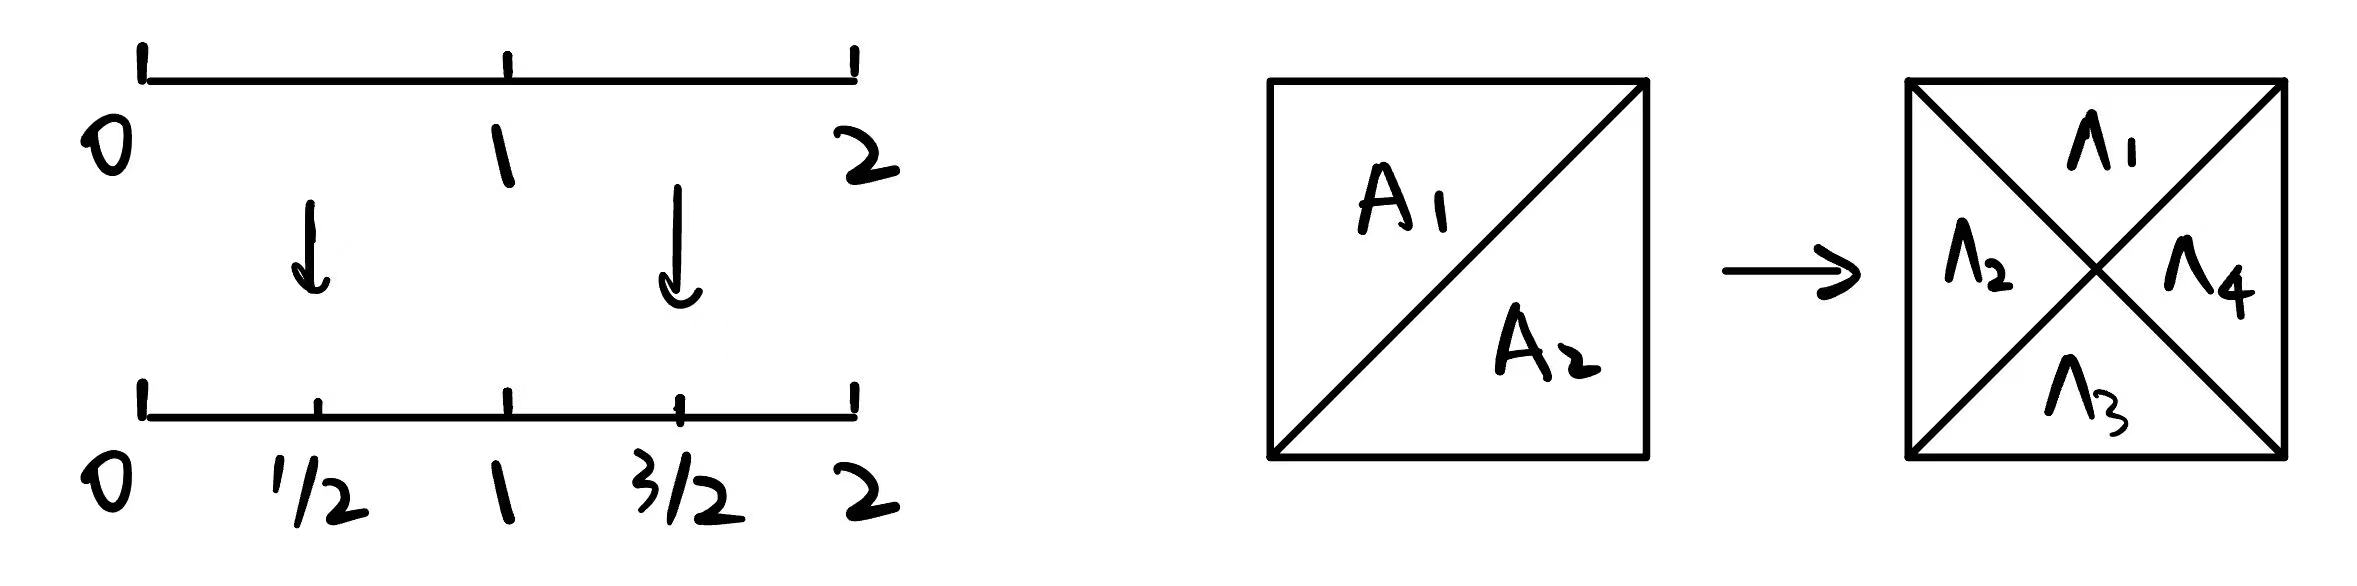
\includegraphics[width=0.8\textwidth]{figures/加细划分.jpg}
    \caption{加细划分}
\end{figure}

(Step 2) 对于 $\omega\in \Lambda_j,\forall j\geq 1$
\[
\begin{aligned}
    \EE(XY|\sigma(\Pi))(\omega) &= \EE(\sum_{k\geq 1}x_k\II_{\Lambda_k}Y|\sigma(\Pi))(\omega)\qquad [X=\sum_{k\geq 1}x_k\II_{\Lambda_k}]\\
    &=\EE(\sum_{k\geq 1}x_k\II_{\Lambda_k}Y|\Lambda_j)\qquad [\sigma(\Pi)\text{定义}]\\
    &=\EE(\sum_{k\geq 1}x_k\II_{\Lambda_k}Y\II_{\Lambda_j})/\PP(\Lambda_j)\qquad [\text{Cor }\eqref{cor:con_exp_indic}]\\
    &=\EE(Yx_j\II_{\Lambda_j})/\PP(\Lambda_j)\qquad [\II_{\Lambda_k}\II_{\Lambda_j}\text{当}\Lambda_k\neq\Lambda_j\text{时}=0]\\
    &=x_j\EE(Y\II_{\Lambda_j})/\PP(\Lambda_j)\\
    &=x_j \EE(Y|\II_{\Lambda_j})\\
    &=X(\omega)\EE(Y|\II_{\Lambda_j})
\end{aligned}
\]

\[
\Rightarrow \EE(XY|\sigma(\Pi))=X\sum_{j\geq 1}\II_{\Lambda_j}\EE(Y|\Lambda_j)=X\EE(Y|\sigma(\Pi))
\]

数学上有种现象叫“法国人的伎俩”, 即把定理当定义用. 严格地讲, 这么做有时会出现存在性和唯一性不满足的问题. 下面介绍一个常被当做定义用的定理: 

\begin{theorem}\label{thm:partition_con_exp}
    $\Pi=\{\Lambda_k,k\geq 1\}$ 为 $\Omega$ 的划分,  $\EE|X|<\infty$. 记 $Y:=\EE(X|\sigma(\Pi))=\sum_{k\geq 1}\II_{\Lambda_k}\EE(X|\Lambda_k)$, 则
    \begin{enumerate}
        \item $Y$ 仍是一个离散随机变量, 且 $\EE|Y|\geq \EE|X|<\infty$
        \item $\sigma(Y)\st \sigma(\Pi)$ (记作 $Y\in \sigma(\Pi)$, 即 $Y$ 的所有信息都在 $\sigma(\Pi)$ 里)
        \item $\forall A\in \sigma(\Pi)$, 有 $\EE(Y\II_A)=\EE(X\II_A)$
    \end{enumerate}
\end{theorem}

证明: (1)$E|X|=\sum_{x\in S_x}|x|\PP(X=x)<\infty$

\[
    \EE|Y|=\sum_{k\geq 1}|\EE(X|\Lambda_k)|\PP(\Lambda_k)\geq \sum_{k\geq 1}\sum_{x\in S}|x|\PP(\{X=x\}\cap \Lambda_k)
\]

逻辑上, 现在第一个等号不成立, 但之后 $<\infty$ 一写出来, 之前的所有等号立刻成立, 此处只为书写简便

\[
    \EE|X|=\sum_{x\in S_x}|x|\PP(X=x)=\sum_{x\in S}|x|\sum_{k\geq 1}\PP(\Lambda_k\cap \{X=x\})
\]

我们知道 $\sum_{x\in S}|x|\sum_{k\geq 1}\PP(\Lambda_k\cap \{X=x\})$ 绝对收敛, 若求和次序交换后的 $\sum_{k\geq 1}\sum_{x\in S}|x|\PP(\{X=x\}\cap \Lambda_k)$ 也绝对收敛, 则 $\EE|Y|<\infty$ 得证. 有一个引理可以保证绝对收敛: 

\begin{lemma}[\cite{calculus}.P280.推论]\label{lem:abs_convergence}
    从 273-280
\end{lemma}

\begin{corollary}\label{cor:double_exp}
    来自Thm \ref{thm:partition_con_exp}(1).
    \begin{enumerate}
        \item (重期望公式)
        \begin{equation}
\EE|\EE(X|\sigma(\Pi))|=\EE|X|, \EE(\EE(X|\sigma(\Pi)))=\EE(X)
\label{eq:double-exp}
\end{equation}
        \item $|\EE(X|\Lambda_k)|\leq \EE(|X|\mid\Lambda_k), |\EE(X|\sigma(\Pi))|\leq \EE(|X|\mid\sigma(\Pi))$
    \end{enumerate}
\end{corollary}

(2) 由定义, $Y=\sum_{k\geq 1}y_k\II_{\Lambda_k}$, 其中 $y_k:=\EE(X|\Lambda_k)$

记 $S_Y=\cup_{k\geq 1}\{y_k\}$, 注意到, 可能 $\exists i\neq j$, 但 $y_i=y_j$

故 $J_y=\{k|y_k=y\}(y\in S_Y)$ 中个数可能大于1

\[
Y=\sum_{y\in S_Y}y\II_{\sum_{k\in J_y}\Lambda_k}
\]

\[
\{Y=y\}=\sum_{k\in J_y}\Lambda_k\in \sigma(\Pi)
\]

\[
\sigma(Y)\st \sigma(\Pi)\qed
\]

(3) $\EE(Y\II_A)=\EE(\II_A\EE(X|\sigma(\Pi)))$

\[
\begin{aligned}
    \EE(Y\II_A)&=\EE(\II_A\EE(X|\sigma(\Pi)))\\
    &=\EE(\EE(X\II_A|\sigma(\Pi)))\qquad [A\in \sigma(\Pi), \text{性质\eqref{prt:extract_known}}]\\
    &=\EE(X\II_A)\qquad [\text{Cor } \eqref{cor:double_exp}]
\end{aligned}
\]

\subsubsection*{$3^\circ$关于离散随机变量的条件期望}

\begin{definition}
    概率空间 $(\Omega,\CF,\PP)$, $X,Y$ 为离散随机变量, $\EE|X|<\infty$. 定义 $\EE(X|Y)=\EE(X|\sigma(Y))=\EE(X|\sigma(\Pi_Y))$, 称为 $X$ 关于 $Y$ 的条件期望
\end{definition}

注: $\omega=\{Y=y\}\in \Pi_Y$ 或 $Y(\omega)=y$, $\EE(X|Y)(\omega)=\EE(X|Y=y)$

\begin{example}
    $\EE(X|\Pi_{\Omega})=\EE(X|\sigma(\Omega))=\EE(X)$
\end{example}

\begin{example}
    $\II_A\ind \II_B\Rightarrow \EE(\II_A|\II_B)=[\text{Exa\eqref{exa:con_exp_indic}}]\EE(\II_A)$
\end{example}

\begin{example}
    $\EE(X|X)=\EE(X|\sigma(X))=X$[\text{Exa \ref{exa:extract_known}}]
\end{example}

\begin{property}
    假设以下期望、条件期望都有意义
    \begin{enumerate}
        \item $\EE(aX+bY|Z)=a\EE(X|Z)+b\EE(Y|Z)$
        \item $X\ind Y\Rightarrow \EE(X|Y)=\EE(X)$
        \item $\sigma(X)\st \sigma(Z)\Rightarrow \EE(XY|Z)=X\EE(Y|Z)$
        \item $\EE(\EE(X|Z))=\EE(X)$
        \item $|\EE(X|Z)|\leq \EE(|X|\mid Z)$
    \end{enumerate}
\end{property}

\subsubsection*{$4^\circ$关于多个离散随机变量的条件期望}

$\EE(Y|X_1,\cdots,X_n)$

\begin{enumerate}
    \item 由 $X_1,\cdots ,X_n$ 生成的 $\sigma$代数 $\sigma(X_1,\cdots,X_n)$
    \item $:=\EE(Y|\sigma(X_1,\cdots ,X_n))$
\end{enumerate}

怎样生成 $\sigma$代数可以包含 $X_1,\cdots,X_n$ 尽可能多的信息?

直觉是 $\bigcup_{k=1}^{\infty}\sigma(X_k)$, 然而它不一定是 $\sigma$代数, 因为它对可列并不封闭. 

每个 \(\sigma(X_k)\) 是一个 \(\sigma\)代数, 因此它对可列并封闭. 

然而, \(\bigcup_{k=1}^{\infty} \sigma(X_k)\) 只是将每个 \(\sigma(X_k)\) 中的集合简单地并在一起, 并没有保证这些集合的可列并仍然在 \(\bigcup_{k=1}^{\infty} \sigma(X_k)\) 中. 

例如, 假设 \(X_k \in \sigma(X_k)\), 那么 \(X_k\) 在 \(\bigcup_{k=1}^{\infty} \sigma(X_k)\) 中, 但 \(\bigcup_{k=1}^{\infty} X_k\) 可能不在 \(\bigcup_{k=1}^{\infty} \sigma(X_k)\) 中, 因为它可能不属于任何一个单独的 \(\sigma(X_k)\). 问题出在 \(\bigcup_{k=1}^{\infty} \sigma(X_k)\) 缺少 $\{\sigma(X_k)\}_{k\geq 1}$ 交互的部分

怎样把 \(\bigcup_{k=1}^{\infty} \sigma(X_k)\) 变成$\sigma$代数?

\begin{definition}[多个离散随机变量生成的$\sigma$-代数]\label{def:multi_rv_con_exp}
    定义由离散随机变量 $X_1,\cdots,X_n$ 生成的 $\sigma$代数
    \[
    \begin{aligned}
        \sigma(X_1,\cdots,X_n)&:=(X_1,\cdots,X_n)^{-1}(2^{S_1}\times \cdots \times 2^{S_n})\\
        &:=\{\underbrace{(X_1,\cdots,X_n)^{-1}(A_1\times\cdots\times A_n)}_{\text{柱集}}|A_1\times\cdots\times A_n\st \underbrace{S_1\times\cdots\times S_n}_{\text{乘积空间}}\}\\
        &=\left\{\bigcap_{k=1}^{\infty}X_k^{-1}(A_k)|A_k\in 2^{S_k},1\leq k\leq n\right\}
    \end{aligned}
    \]
\end{definition}

\begin{theorem}\label{thm:discrete_rv_partition}
    令 $x_k=\sum_{i\geq 1}x_{k,i}\II_{\Lambda_{k,i}}, 1\leq k\leq n$, 为离散随机变量, 对每一个 $k$, $\Pi_k:=\{\Lambda_{k,i}|i\geq 1\}$ 为 $\Omega$ 的划分, 定义
    \[
    \Pi_{(X_1,\cdots,X_n)}:=\{\Lambda_{1,i_1}\cap\cdots \cap \Lambda_{n,i_n}|i_k\geq 1,1\leq k\leq n\}
    \]
    则
    \begin{enumerate}
        \item $\Pi_{(X_1,\cdots,X_n)}$ 是 $\Omega$ 的划分, 且
        \[
            \sigma(\Pi_{(X_1,\cdots,X_n)})=\left \{\sum_{\substack{(i_1,\cdots ,i_n) \\ \in J_1\times \cdots \times J_n}} (\Lambda_{1,i_1}\cap \cdots \cap \Lambda_{1,i_n})|J_k\st \NN,1\leq k\leq n\right \}
        \]
        \item $\sigma(X_1,\cdots,X_n)=\sigma(\Pi_{(X_1,\cdots ,X_n)})$ (即定义\ref{def:multi_rv_con_exp}是有意义的, well-defined, make sense, 良定义) 
    \end{enumerate}
\end{theorem}

\begin{problem}[作业2-2]
    证明Theorem \ref{thm:discrete_rv_partition}在 $n=2$ 时成立
\end{problem}

\begin{definition}
    $\EE|Z|<\infty$ 定义
    \[
    \EE(Z|X_1,\cdots,X_n)=\EE(Z|\sigma(X_1,\cdots,X_n)):=\EE(Z|\sigma(\Pi_{(X_1,\cdots,X_n)}))
    \]
\end{definition}

\begin{definition}\label{def:multi_rv_indep}
    $(\Omega,\CF,\PP), Y:\Omega\to S_Y, X_1:\Omega\to S_1,X_2:\Omega\to S_2$ 为离散随机变量, 称 $Y$ 和 $(X_1,X_2)$ 独立, 若 $\sigma(Y)\ind \sigma(X_1,X_2)$. [$\sigma(Y)=Y^{-1}(2^{S_Y}),\sigma(X_1,X_2)=(X_1,X_2)^{-1}(2^{S_1}\times 2^{S_2})$]

    即 $\forall A\st S_Y,B\st 2^{S_1}\times 2^{S_2}, B=B_1\times B_2$, 有 
    \[
    \PP(Y\in A,(X_1,X_2)\in B)=\PP(Y\in A)\PP((X_1,X_2)\in B)
    \]
    其中 $\PP((X_1,X_2)\in B)=\PP(X_1\in B_1,X_2\in B_2)$
\end{definition}

\begin{problem}[作业2-3]
    证明: 
    \[
    \begin{aligned}
        Y\ind (X_1,X_2)\Leftrightarrow &\forall y\in S_Y,x_1\in S_1,x_2\in S_2\\
        &\text{有}\PP(Y=y,(X_1,X_2)=(x_1,x_2))\\
        &=\PP(Y=y)\PP((X_1,X_2)=(x_1,x_2))
    \end{aligned}
    \]
\end{problem}

有了上述定义, 可以推广: 

\begin{enumerate}
    \item $(Y_1,\cdots,Y_n)\ind (X_1,\cdots,X_n)$
    \item $Y\ind_A (X_1,\cdots,X_n) (A\in \CF,\PP(A)>0)$
\end{enumerate}

\begin{property}\label{prop:pairwise_indep}
    $Y\ind (X_1,X_2)\Rightarrow Y\ind X_1,Y\ind X_2$
\end{property}

证明: 在 Def \ref{def:multi_rv_indep}中取$B_2=\Omega$

\[
\begin{aligned}
    \PP(Y\in A,X_1\in B_1)&=\PP(Y\in A,X_1\in B_1,X_2\in S_2)\\
    &=\PP(Y\in A)\PP(X_1\in B_1,X_2\in S_2)\qquad [Y\ind (X_1,X_2)]\\
    &=\PP(Y\in A)\PP(X_1\in B_1)
\end{aligned}
\]

注: 看到 $\Rightarrow$ 要自然地问, 反过来 $\Leftarrow$ 成立吗?做数学要多问自己一些问题, 即便没有答案

\begin{corollary}
    $(Y_1,\cdots,Y_n)\ind (X_1,\cdots,X_n)\Rightarrow Y_k\ind X_j, 1\leq k\leq m,1\leq j\leq n$
\end{corollary}
\newpage
\subsection{随机过程}

\subsubsection{什么是随机过程}

\begin{definition}[随机过程]
    设 $(\Omega, \CF, \PP)$ 为概率空间, $(S,\CS)$ 为可测空间, $\TT$ 为指标集/参数集, 称随机变量族
    \[
    \{X_t: (\Omega,\CF,\PP)\rightarrow (S,\CS)|t\in \TT\}
    \]
    为 (S值) 随机过程 $X$. 其中 $(S,\CS)$ 称为 $X$ 的状态空间

    注: \begin{enumerate}
        \item $forall t\in \TT$, $X_t$ 为随机变量
        \item $\TT$ 为时间集, $X_t$ 为过程 $X$ 在时刻 $t$ 的状态
    \end{enumerate}
\end{definition}

\[
\begin{array}{c|cc}
    \TT \backslash S \st \RR & \text{离散 }(e.g.\ \NN) & \text{连续 }(e.g.\ \RR,\RR^+) \\ \hline
    \text{可数集 }(e.g.\ \NN,\ZZ) & \multicolumn{2}{c}{\text{离散时间/参数的随机过程}} \\
    \text{连续统 }(e.g.\ [0,T],\RR^+) & \multicolumn{2}{c}{\text{连续时间/参数的随机过程}}
\end{array}
\]

\subsubsection{随机过程的分布}

\begin{enumerate}
    \item $\forall t\in \TT, X_t:\Omega\rightarrow S$ 为随机变量/可测映射
    \item $X: \TT\times \Omega\rightarrow S$ 二元映射
    \item $X:\Omega\rightarrow S^{\TT}$ 其中 $S^{\TT}=\{f|f:\TT\rightarrow \S\}$, $X:\omega\rightarrow X(\omega)=X(\cdot,\omega)$
\end{enumerate}

分布可用有限维分布族刻画

\begin{definition}
    固定样本点 $\omega$, 则 $X_{\cdot}(\omega)$ 为 $\TT\rightarrow S$ 的映射, 即 $X_{\cdot}(\omega)\in S^{\TT}$, 称 $X_{\cdot}(\omega)$ 是过程 $X$ 的一个实现/样本路径/样本函数
\end{definition}

\begin{definition}
    $\forall n\geq 1, t_1,t_2,\cdots,t_n$ 称 
    \[
    (x_1,x_2,\cdots,x_n)\mapsto F_{t_1,t_2,\cdots,t_n}(x_1,x_2,\cdots,x_n)=\PP(X_{t_1}\leq x_1,\cdots, X_{t_n}\leq x_n)
    \]
    为 $X$ 的 $n$ 维分布
\end{definition}

\begin{definition}[过程的有限维分布族]
    定义
    \[
    \{F_{t_1,t_2,\cdots,t_n}|n\geq 1,t_1,\cdots,t_n\in \TT\}
    \]
\end{definition}

\subsubsection{随机过程的存在性}

\begin{enumerate}
    \item (抽象的) 从概率论/测度论出发去证明随机过程存在性, 不写出具体形式, 满足随机过程符合给定的有限维分布族即可
    \item (具体的) 构造性证明
\end{enumerate}

\begin{property}
随机过程的有限维分布族具有以下两个性质
\begin{enumerate}
    \item (对称性) 重排, 设 $\sigma:\{1,\cdots,n\}\rightarrow \{1,\cdots,n\}$ 为双射, 则
    \[
    F_{t_{\sigma(1)}, \cdots,t_{\sigma(n)}}(x_{\sigma(1)},\cdots,x_{\sigma(n)})=F_{t_1,\cdots,t_n}(x_1,\cdots,x_n)
    \]
    \item (相容性) $m\geq n$
    \[
    F_{t_1,\cdots,t_n,t_{n+1},\cdots,t_m}(x_1,\cdots,x_n,+\infty,\cdots,+\infty)=F_{t_1,\cdots,t_n}(x_1,\cdots,x_n)
    \]
    注: 相容性类比从高维向低维的投影, $\PP(X\leq +\infty)=F_X(+\infty)=1$
\end{enumerate}
这两个性质是随机过程存在的必要条件
\end{property}

\begin{theorem}[Kolmogorov定理]\label{thm:Kolmogorov}
    设分布函数族
    \[
    \{F_{t_1,\cdots,t_n}|t_1,\cdots,t_n\in \TT,n\geq 1\}
    \]
    满足\uwave{对称性}, \uwave{相容性}, 则必存在一个随机过程 $\{X_t,t\in \TT\}$ 使得上述分布函数族 $F$ 是 $X$ 的有限维分布族
\end{theorem}

\subsubsection{随机过程的基本类型}

\begin{enumerate}
    \item 离散时间马氏链 (由条件概率定义) 
    \item Poisson 过程
    \item 更新过程
    \item 连续时间马氏链
    \item 离散时间 Martingale  (由条件期望定义) 
    \item 布朗运动
\end{enumerate}

\begin{definition}
    对连续时间的随机过程 $\{X_t,t\in \TT\}$
    \begin{enumerate}
        \item 若对一切的 $t_0<t_1<\cdots<t_n$ 有 $X_{t_1}-X_{t_0},\cdots,X_{t_n}-X_{t_{n-1}}$ 相互独立, 则过程 $X$ 是独立增量过程 (e.g. 布朗运动) 
        \item 若对每一个 $S\in \TT, X_{t+s}-X_t$ 对一切的 $t$ 都有相同分布, 称 $X$ 为平稳增量过程
    \end{enumerate}
\end{definition}

\pagebreak

\section{马氏链}
\subsection{离散时间马氏链}

马尔可夫性 $\leftrightarrow$ 已知现在, 过去与未来不相干/独立

\begin{definition}[(离散时间)马氏链]\label{def:M_1}
    称 $S$ 值随机过程 $\{X_n,n\geq 0\}$ 为马氏链, 若 $X$ 满足以下马氏性:$\forall n\geq 0,x_0,x_1,\cdots,x_n,y\in S$, 
    \begin{equation}
\PP(\underbrace{X_{n+1}=y}_{\text{未来}}|\underbrace{X_0=x_0,\cdots,X_{n-1}=x_{n-1}}_{\text{过去}},\underbrace{X_n=x_n}_{\text{现在}})=\PP(X_{n+1}=y|X_n=x_n)
\label{eq:M1}
\tag{$M_1$}
\end{equation}
    其中 $X_0$ 的分布称为 $X$ 的初始分布
\end{definition}

\begin{definition}
    当 $S$ 为有限集, 称链为有限链, 当 $S$ 为无限集, 称链为无限链
\end{definition}

注:改写 $(M_1)$
\[
LHS=\PP_{X_n=x_n}(X_{n+1}=y|X_0=x_0,\cdots,X_{n-1}=x_{n-1})
\]
\[
RHS=\PP_{X_n=x_n}(X_{n+1}=y)
\]
\[
\begin{aligned}
    M_1 &\Leftrightarrow \{X_{n+1}=y\}\ind_{\{X_n=x_n\}}\{X_0=x_0,\cdots,X_{n-1}=x_{n-1}\}\\
    &\Leftrightarrow X_{n+1}\ind_{\{X_n=x_n\}} (X_0,\cdots,X_{n-1})
\end{aligned}
\]
$(M_1)\quad \text{未来}\ind_{\text{现在}}\text{过去}$
\[
\PP_{\text{现在}}(\text{未来}|\text{过去})=\PP_{\text{现在}}(\text{未来})
\]

\begin{lemma}[马氏性的等价表示]\label{lem:markov_equiv}
    [Grimmett\cite{grimmett}] 下面三个命题等价
    \begin{enumerate}
        \item $(M_1)$ 马氏性
        \item $(M_2)$ $\forall k\geq 0, 0\leq n_1< \cdots<n_k\leq n$, 对于 $y,x_{n_1},\cdots,x_{n_k}\in S$, 
        \begin{equation}
				\PP(X_{n+1}=y|X_{n_1}=x_{n_1},\cdots,X_{n_k}=x_{n_k})=\PP(X_{n+1}=y|X_{n_k}=x_{n_k})
				\label{eq:markov_equiv_M2}
				\end{equation}
        即
        \[
        \{X_{n+1}=y \}\ind_{\{X_{n_k}=x_{n_k}\}}\{X_{n_1}=x_{n_1},\cdots,X_{n_{k-1}}=x_{n_{k-1}}\}
        \]
        \item $(M_3)$ 对 $\forall m\geq 1,n\geq 0, \{y,x_i,0\leq i\leq n\}\st S$, 有
        \begin{equation}
        \PP(X_{n+m}=y|X_0=x_0,\cdots,X_n=x_n)=\PP(X_{n+m}=y|X_n=x_n)
        \label{eq:markov_equiv_M3}
        \end{equation}
        即
        \[
        \{X_{n+m}=y\}\ind_{\{X_n=x_n\}}\{X_0=x_0,\cdots,X_{n-1}=x_{n-1}\}
        \]
    \end{enumerate}
\end{lemma}

证明:思路 $1\leftrightarrows 3\leftrightarrows 2$

$(2)\rightarrow (3)$, 先处理一些记号的问题.记(2)中的 $n$ 为 $n^{(2)}$, (3)中的 $n$ 为 $n^{(3)}$.则取 $n_k=n^{(3)}=n^{(2)}+1-m\leq n^{(2)}$, 所以 $n^{(3)}+m=(n^{(2)}+1-m)+m=n^{(2)}+1$, 即已知(2)可推(3)

$(3)\rightarrow (1)$, 取 $m=1$, 显然

只需证 $(3)\rightarrow (2),(1)\rightarrow (3)$

这里回顾独立的三种写法
\begin{enumerate}
    \item $A\ind_B C$ 记号
    \item $\PP_B(A,C)=\PP_B(A)\PP_B(C)$ 定义
    \item $\PP_B(A|C)=\PP_B(A)$ 定理
\end{enumerate}

(Step 1) 证明 $(3)\rightarrow (2)$

思路:(2)(3)条件不同, 想要由(3)推(2), 则切换到(2)的条件概率测度, 展开, 再用(3)的条件瘦身

对 $\forall k\geq 2, 0\leq n_1<n_2<\cdots<n_k=n$

令 $J=\{0,1,\cdots,n_k-1,n_k\}\backslash \{n_1,\cdots,n_k\}$, $\tilde{\PP}(\cdot)=\PP(\cdot|X_{n_1}=x_{n_1},\cdots,X_{n_k}=x_{n_k})$

\[
\begin{aligned}
    \tilde{\PP}(X_{n+1}=y)&=\sum_{x_j\in S,j\in J}\tilde{\PP}(X_{n+1}=y|X_j=x_j,j\in J)\cdot\tilde{\PP}(X_j=x_j,j\in J)\qquad [\text{全概公式}]\\
    &=\PP(X_{n+1}=y|X_{n_k}=x_{n_k})\sum_{x_j\in S,j\in J}\tilde{\PP}(X_j=x_j,j\in J)\qquad [(3), \PP_C(\cdot|A)=\PP_C(\cdot)]\\
    &=\PP(X_{n+1}=y|X_{n_k}=x_{n_k})
\end{aligned}
\]

其中, 记号 $\sum_{x_j\in S,j\in J}$ 中的下标意为:假设 $J$ 中元素个数为 $\# J=u$, 则 $(x^{(1)},\cdots, x^{(u)})\in S^u$.从简单的开始, $\sum_{x\in S}\PP(X=x)=\PP(\Omega), \sum_{(x,y)\in S^2}\PP(X=x,Y=y)=\PP(\Omega),\cdots$, $\sum_{(x^{(1)},\cdots, x^{(u)})\in S^u}\PP(X^{(1)}=x^{(1)},\cdots,X^{(u)}=x^{(u)})=\PP(\Omega)=1$

(Step 2) 下证 $(1)\rightarrow (3)$

1. $m=1$ 时, 即 $(1)$

2. 假设 $m=k$ 时 $(3)$ 成立, 即 $\forall n\geq 1, \{y,x_i,n\geq i\geq 0\}\st S$,
\[
\{X_{n+k}=y\}\ind_{\{X_n=x_n\}}\{X_0=x_0,\cdots, X_{n-1}=x_{n-1}\}\xrightarrow{\text{性质\eqref{prop:pairwise_indep}}}\{X_{n+k}=y\}\ind_{\{X_n=x_n\}}\{X_{n-1}=x_{n-1}\}
\]
\[
\begin{aligned}
    \PP(X_{n+k}=y|X_0=x_0,\cdots,X_n=x_n)&=\PP(X_{n+k}=y|X_n=x_n)\\
    &=\PP(X_{n+k}=y|X_n=x_n,X_{n-1}=x_{n-1})
\end{aligned}\tag{*}
\]
当 $m=k+1$ 时, 对 $\forall \{y,x_i,n\geq i\geq 0\}\st S$

令 $\tilde{\PP}_n(\cdot):=\PP(\cdot|X_0=x_0,\cdots,X_n=x_n)$
\[
\begin{aligned}
    \tilde{\PP}_n(X_{n+k+1}=y)&\overset{\text{Thm}\eqref{thm:law_total_prob}}{=}\sum_{x_{n+1}\in S}\tilde{\PP}_n(X_{n+k+1}=y|X_{n+1}=x_{n+1})\cdot \tilde{\PP}_n(X_{n+1}=x_{n+1})\\
    &=\sum_{x_{n+1}\in S}\PP(X_{n+k+1}=y|X_{n+1}=x_{n+1},X_n=x_n)\cdot \PP(X_{n+1}=x_{n+1}|X_n=x_n)\quad [\text{(*), 归纳法假设}]\\
    &\overset{\eqref{eq:multiply_func}}{=}\sum_{x_{n+1}\in S}\PP(X_{n+k+1}=y,X_{n+1}=x_{n+1},X_n=x_n)/\PP(X_n=x_n)\\
    &=\PP(X_{n+k+1}=y,X_n=x_n)/\PP(X_n=x_n)\\
    &=\PP(X_{n+k+1}=y|X_n=x_n)
\end{aligned}
\]
即 $m=k+1$ 得证\qed

证明 (Step 2) 时如果在 $x_{n+k}$ 处展开而不是在 $x_{n+1}$, 也是可以的.实际上在 $x_{n+j}, \forall j, 1\leq j\leq k$ 展开都可以, 关键在于用性质\ref{prop:pairwise_indep}和全概公式\ref{thm:law_total_prob}凑出乘法公式\eqref{eq:multiply_func}, 消元即可.

\begin{remark}
    三种写法的直觉
    \begin{enumerate}
        \item $M_1$:未来“下一步”跟过去“每一步”都无关
        \item $M_2$:未来“下一步”跟过去的“任意若干步”都无关
        \item $M_3$:未来“下m步”跟过去“每一步”都无关
    \end{enumerate}
    可以推出, 由(2)(3), 下式也成立:
    
    对 $\forall m\geq 1,n\geq 0, \{y,x_i,0\leq i\leq n\}\st S$
    \[
    \PP(X_{n+m}=y|X_{n_1}=x_{n_1},\cdots,X_{n_k}=x_{n_k})=\PP(X_{n+m}=y|X_{n_k}=x_{n_k})
    \]
\end{remark}

\begin{corollary}\label{cor:markov_con_cut}
    若 $X$ 是马氏链, 则 $\forall n\geq 1,\{x_i,n\geq i\geq 0,y\}\st S$, 有 
    \[
    \PP(X_{n+1}=y|X_0=x_0,\cdots,X_n=x_n)=\PP(X_{n+1}=y|X_n=x_n,X_{n-1}=x_{n-1})
    \]
\end{corollary}

补充记号:
\begin{itemize}
    \item 乘积空间
    \[
        S^n:=\underbrace{S\times\cdots\times S}_{\text{n个}}
    \]
    \item 乘积 $\sigma$ 代数
    \[
        \bigotimes_n 2^S:=\underbrace{2^S\times\cdots\times 2^S}_{\text{n个}}
    \]
\end{itemize}

\begin{property}[马氏性的等价条件]\label{prt:markov_equiv_condition}
下列三个命题等价
\begin{enumerate}
    \item 马氏性 $(M_1)$
    \item 对 $\forall n\geq 1,m\geq 1,A\in \otimes_n 2^S,B\in \otimes_m 2^S$, 即 $(A\st S^n,B\st S^m)$, 有
    \begin{equation}
    \begin{aligned}
        &\PN((X_0,\cdots,X_{n-1})\in A,(X_{n+1},\cdots,X_{n+m})\in B)\\
        =&\PN((X_0,\cdots,X_{n-1})\in A)\cdot \PN((X_{n+1},\cdots,X_{n+m})\in B)
    \end{aligned}
    \label{eq:markov_equiv_condition_M2}
    \end{equation}
    即 $(X_0,\cdots,X_{n-1})\ind_{\{X_n=x_n\}}(X_{n+1},\cdots,X_{n+m})$ 的定义
    \item $\PN((X_{n+1},\cdots,X_{n+m})\in B|(X_0,\cdots,X_{n-1})\in A)=\PN((X_{n+1},\cdots,X_{n+m})\in B)$
\end{enumerate}
\end{property}

证明:$(2)\Leftrightarrow (3)$, 独立的定义和定理, 显然

$(3)\rightarrow (1)$, 取 $k=0$ 显然

只需证 $(1)\rightarrow (3)$

只需证 $(3)$ 对简单事件 $A,B$ (单点集合) 成立, 即 $\forall n\geq 1,m\geq 1, \{x_0,x_1,\cdots,x_{n+m}\st S\}$, 有
\[
\PN((X_{n+1},\cdots,X_{n+m})=x_{n+1}^{n+m}|(X_0,\cdots,X_{n-1})=x_0^{n-1})=\PN((X_{n+1},\cdots,X_{n+m})=x_{n+1}^{n+m})
\]
其中 $x_{n+1}^{n+m}=(x_{n+1},\cdots,x_{n+m}),x_{0}^{n-1}=(x_0,\cdots,x_{n-1})$

*只要对单点集合成立, 对一般情况也成立, 证明见Theorem \ref{thm:independent_rv}

令
\[
\tilde{\PP}_n(\cdot):=\PN(\cdot|(X_0,\cdots,X_{n-1})=x_0^{n-1})=\PP(\cdot|(X_0,\cdots,X_{n})=x_0^{n})
\]
只证 $m=2$, 即由
\[\tilde{\PP}_n(X_{n+1}=x_{n+1})=\PP_{\{X_n=x_n\}}(X_{n+1}=x_{n+1})\] 
证得
\[\tilde{\PP}_n(X_{n+1}=x_{n+1}, X_{n+2}=x_{n+2})=\PP_{\{X_n=x_n\}}(X_{n+1}=x_{n+1}, X_{n+2}=x_{n+2})\]
\[
\begin{aligned}
    \tilde{\PP}_n((X_{n+1},X_{n+2})=(x_{n+1},x_{n+2}))&=\tilde{\PP}_n(X_{n+1}=x_{n+1})\cdot \tilde{\PP}_n(X_{n+2}=x_{n+2}|X_{n+1}=x_{n+1})\\
    &\overset{\eqref{eq:M1}}{=}\PP(X_{n+1}=x_{n+1}|X_n=x_n)\cdot \PP(X_{n+2}=x_{n+2}|X_{n+1}=x_{n+1})\\
    &\overset{\text{Cor}\eqref{cor:markov_con_cut}}{=}\PP(X_{n+1}=x_{n+1}|X_n=x_n)\cdot \PP(X_{n+2}=x_{n+2}|X_{n+1}=x_{n+1},X_n=x_n)\\
    &=\PN(X_{n+1}=x_{n+1})\cdot \PN(X_{n+2}=x_{n+2}|X_{n+1}=x_{n+1})\\
    &\overset{\eqref{eq:multiply_func}}{=}\PN((X_{n+1},X_{n+2})=(x_{n+1},x_{n+2}))
\end{aligned}
\]

\begin{corollary}
    设 $X$ 为马氏链, 则对每一个 $n\geq 1,m\geq 1, u_k<u_{k+1}, 0\leq k\leq n+m-1$, 有
    \[
    (X_{u_0},\cdots,X_{u_{n-1}})\ind_{\{X_{u_n}=x_{u_n}\}}(X_{u_{n+1}},\cdots,X_{u_{n+m}})
    \]
\end{corollary}

\newpage
\subsection{时齐马氏链与转移概率}

\begin{definition}[时间齐次马氏链]
    称马氏链 $X:\{X_n,n\geq 0\}$ 为时齐的或时间齐次马氏链, 若对 $\forall n\geq 0, i,j\in S$
    \[
    \PP(X_{n+1}=j|X_n=i)=\PP(X_1=j|X_0=i)
    \]
\end{definition}

\begin{definition}
    $X$ 是时齐马氏链, 称
    \[
    p_{ij}:=p_{i,j}=\PP(X_1=j|X_0=i)\qquad i,j\in S
    \]
    为 $X$ 从状态 $i$ 到 $j$ 的(一步)\textbf{转移概率}, 并称矩阵
    \[
    P=\begin{bmatrix}
        p_{11} & p_{12} & p_{13} & \cdots\\
        p_{21} & p_{22} & p_{23} & \cdots\\
        \vdots & \vdots & \vdots & \ddots
    \end{bmatrix}
    \]
    为(一步)转移(概率)矩阵
\end{definition}

若不加说明, 则默认讨论的马氏链都是时齐的

注:
\[
\begin{aligned}
    \PP(x_{n+1}=y)&=\sum_{x\in S}\PP(X_{n+1}=y|X_n=x)\cdot \PP(X_n=x)\\
    &=\sum_{x\in S}p_{xy}\cdot \PP(X_n=x)
\end{aligned}
\]

\begin{theorem}[转移矩阵的刻画]\label{thm:random_matrix}
    转移矩阵是一个随机矩阵, 即
    \begin{enumerate}
        \item $\forall i,j\in S,p_{ij}\geq 0$
        \item $\forall i\in S,\sum_{j\in S}p_{ij}=1$
    \end{enumerate}
    即转移矩阵的每一行 $(p_{ij})_{j\in S}$ 为 $S$ 上的一个概率分布

    注:另一种随机矩阵是指元素为随机变量的矩阵, 和这里讲的没有关系
\end{theorem}

证明:
\[
\sum_{j\in S}\PP(X_1=j|X_0=i)=\PP(X_1\in S|X_0=i)=\PP(\Omega|X_0=i)=1
\]

\begin{definition}[时齐马氏链]\label{def:homo-markov}
    设 $X=\{X_n,n\geq 0\}$ 为一随机过程, 若
    \begin{enumerate}
        \item 初值 $X_0$ 满足分布 $\mu=(\mu_i)_{i\in S}$, 即 $\PP(X_0=i)=\mu_i,i\in S$
        \item 存在一个随机矩阵 $P=(p_{ij})_{i,j\in S}$ 使得 $\forall n\geq 1,i_0,\cdots,i_{n-1},i,j\in S$
        \[
        \PP(X_{n+1}=j|X_0=i_0,\cdots,X_{n-1}=i_{n-1},X_n=i)=p_{ij}
        \]
    \end{enumerate}
    则称 $X$ 具有初始分布 $\mu$ 和转移矩阵 $P$ 的(时齐)马氏链, 记作 $X\sim \text{Markov}(\mu,P)$
\end{definition}

上述定义与$(M_1)$马氏链定义\ref{def:M_1}等价

证明:$(2)\rightarrow (M_1)$
\[
\begin{aligned}
    \PP(X_{n+1}=j|X_n=i)&=\sum_{(i_0,\cdots,i_{n-1})\in S^n}\PP(X_{n+1}=j|X_n=i,X_0=i_0,\cdots,X_{n-1}=i_{n-1})\PP(X_0=i_0,\cdots,X_{n-1}=i_{n-1})\\
    &=\sum_{(i_0,\cdots,i_{n-1})\in S^n}p_{ij}\cdot \PP(X_0=i_0,\cdots,X_{n-1}=i_{n-1})=p_{ij}
\end{aligned}
\]
所以 $\PP(X_{n+1}=j|X_0=i_0,\cdots,X_{n-1}=i_{n-1},X_n=i)=\PP(X_{n+1}=j|X_n=i)$

即然有 $(M_1)$, 为什么还要定义\ref{def:homo-markov}?因为该定义决定了马氏链的有限维分布

\begin{example}[Gambler's Ruin]
    [Durrett\cite{durrett},P1] 
    \begin{figure}[H]
        \centering
        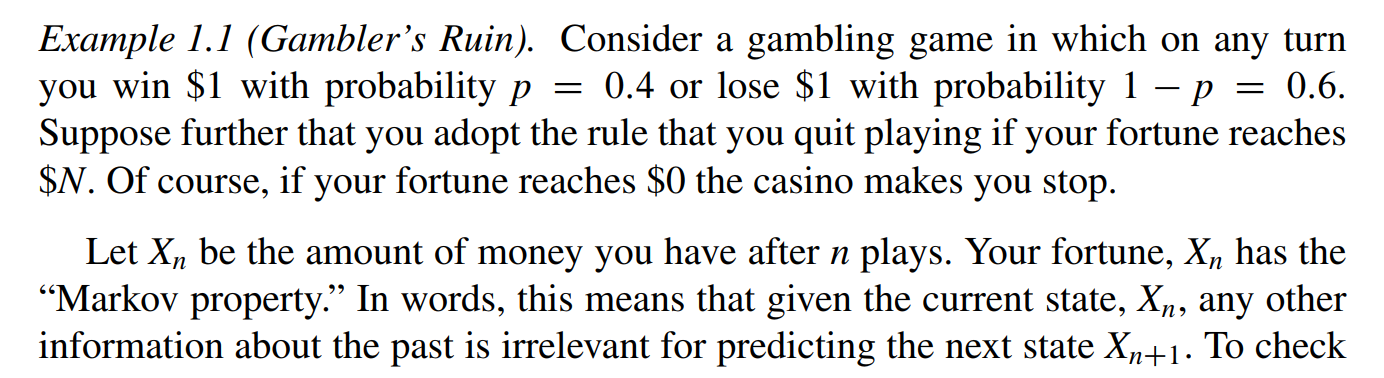
\includegraphics[width=0.9\textwidth]{figures/Gambler's Ruin.png}
        \caption{Gambler's Ruin}
    \end{figure}
\end{example}

\begin{claim}
$\{X_n,n\geq 0\}$ 为(时齐)马氏链
\end{claim}

1. 对于 $0<i_0,\cdots,i_{n-1}<N, n\geq 0$ 有
\[
\begin{aligned}
    &\PP(X_{n+1}=i+1|X_n=i,X_0=i_0,\cdots,X_{n-1}=i_{n-1})\\
    =&\PP(X_{n+1}=i+1|X_n=i)=0.4=\PP(\text{第}n+1\text{次赌局赢一元})
\end{aligned}
\]
\[
\begin{aligned}
    &\PP(X_{n+1}=i-1|X_n=i,X_0=i_0,\cdots,X_{n-1}=i_{n-1})\\
    =&\PP(X_{n+1}=i-1|X_n=i)=0.6=\PP(\text{第}n+1\text{次赌局输一元})
\end{aligned}
\]

2. $\PP(X_{n+1}=0|X_n=0,X_0=i_0,\cdots,X_{n-1}=i_{n-1})=1=\PP(X_{n+1}=0|X_n=0)$

$\PP(X_{n+1}=N|X_n=N, X_0=i_0,\cdots, X_{n-1}=i_{n-1})=1=\PP(X_{n+1}=N|X_n=N)$

最后一个等号是由题目设定得到, 从 $0\to 0$ 或 $N\to N$ 的概率都为1, 因为游戏结束

综上, $p(i,i+1)=0.4,0<i<N, p(i,i-1)=0.6, 0<i<N, p(0,0)=p(N,N)=1$

e.g. 

\begin{figure}[H]
    \centering
    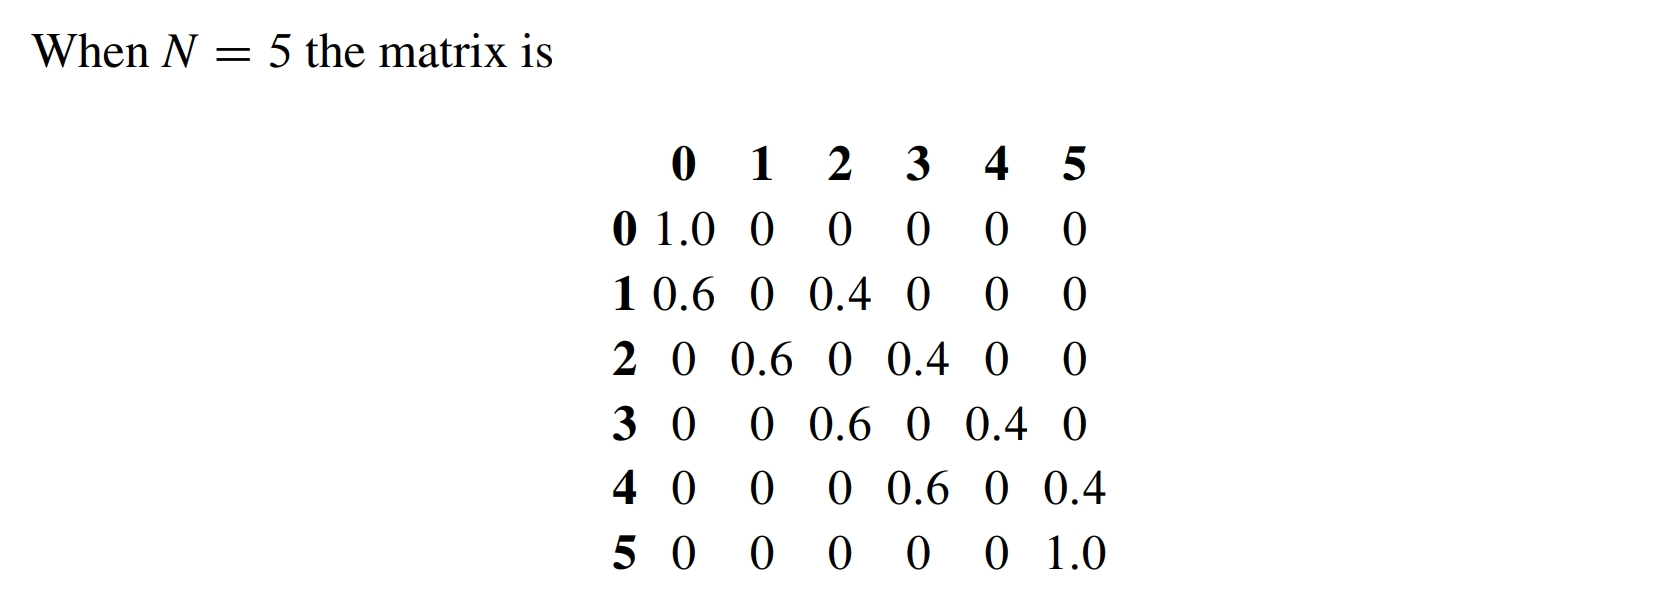
\includegraphics[width=0.9\textwidth]{figures/N=5.png}
    \caption{N=5}
\end{figure}

\begin{example}[Two-Stage Markov Chains]
    [Durrett\cite{durrett}, P7]
    \begin{figure}[H]
        \centering
        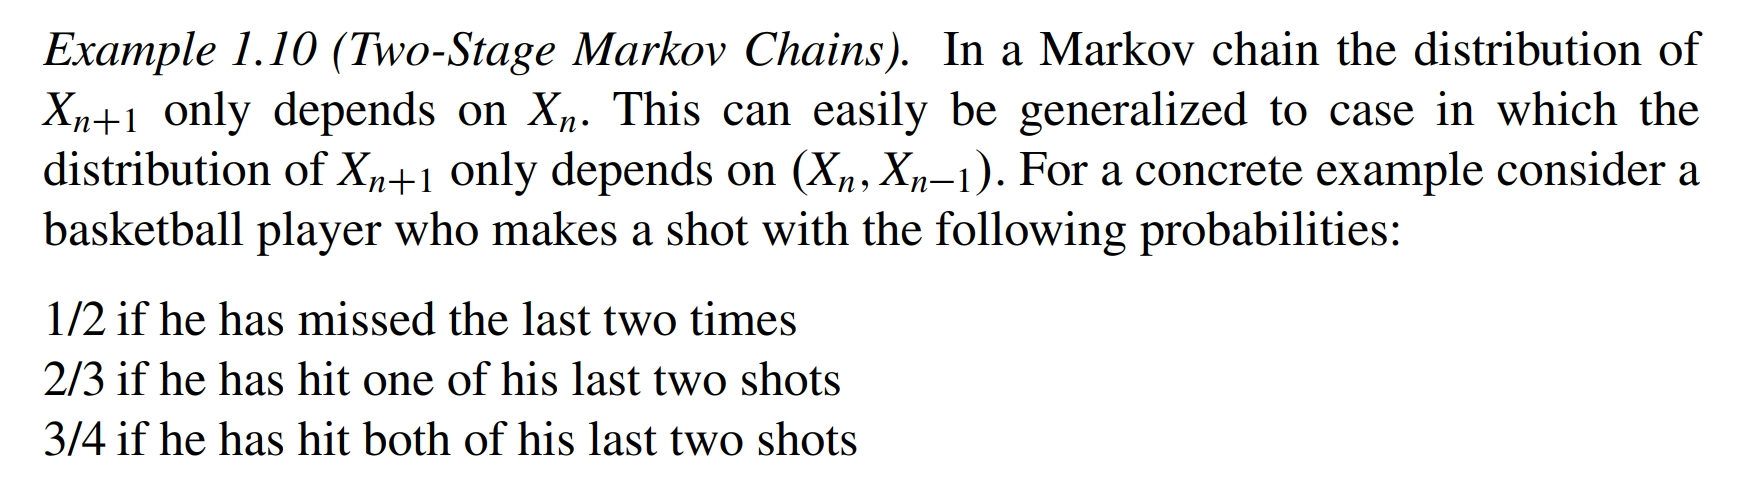
\includegraphics[width=0.9\textwidth]{figures/two_stage_markov_chains.png}
        \caption{Two-Stage Markov Chains}
    \end{figure}
\end{example}

\begin{enumerate}
    \item $\PP(X_{n+1}=H|X_n=M,X_{n-1}=M)=1/2$
    \item $\PP(X_{n+1}=H|X_n=M,X_{n-1}=H)=\PP(X_{n+1}=H|X_n=H,X_{n-1}=M)=2/3$
    \item $\PP(X_{n+1}=H|X_n=H,X_{n-1}=H)=3/4$
\end{enumerate}

\begin{claim}
$Y_n=(X_n,X_{n-1}), n\geq 1$ 则 $\{Y_n,n\geq 1\}$ 是(时齐)马氏链, $Y_n:\Omega\to \{HH,HM,MH,MM\}$ 
\end{claim}

证明:
\[
\begin{aligned}
    &\PP(Y_{n+1}=HH|Y_n=HH,Y_j=(x_j,x_{j-1}), 1\leq j\leq n-1)\\
    =& \PP(X_{n+1}=H,X_n=H|X_n=H,X_{n-1}=H,X_j=x_j,X_{j-1}=x_{j-1},0\leq j\leq n-1)\\
    =& \PP(X_{n+1}=H|X_n=H,X_{n-1}=H)\\
    =&3/4\qquad [3.]
\end{aligned}
\]

对 1.2. 同理\qed

\begin{proposition}[初见马氏链的有限维分布]\label{prop:markov_dist}
设 \(P = (p_{ij})_{i,j \in S}\) 为随机矩阵, \(\mu = (\mu_i)_{i \in S}\) 为概率分布, \(X = \{X_n, n \geq 0\}\) 为 \(S\) 值离散时间随机过程.则过程 \(X \sim \text{Markov}(\mu, P)\) 当且仅当对任意的 \(n \geq 0, i_0, i_1, \cdots, i_n \in S\), \(X\) 有有限维分布:
\begin{equation}
\PP(X_0 = i_0, X_1 = i_1, \cdots, X_n = i_n) = \mu_{i_0} \prod_{k=0}^{n-1} p_{i_k i_{k+1}}
\label{eq:markov_dist}
\end{equation}

\end{proposition}

证明:$\Rightarrow$ 
\[
\begin{aligned}
    &\PP(X_0=i_0,X_1=i_1,\cdots,X_n=i_n)\\
    =&\PP(X_0=i_0)\PP(X_1=i_1|X_0=i_0)\cdots \PP(X_n=i_n|X_0=i_0,\cdots X_{n-1}=i_{n-1})\quad [\text{乘法公式}\eqref{eq:multiply_func}]\\
    =&\PP(X_0=i_0)\PP(X_1=i_1|X_0=i_0)\cdots \PP(X_n=i_n|X_{n-1}=i_{n-1})\quad [\text{Markov}]\\
    =&\mu_{i_0}p_{i_0,i_1}\cdots p_{i_{n-1},i_n}
\end{aligned}
\]
严格地讲, $\PP(\cdot|A)$ 需保证 $\PP(A)>0$.对 $\PP(A)=0$ 情况的分类讨论, 见 Resnick\cite{resnick}, prop 2.1.1

$\Leftarrow$ 

1. $n=0, \PP(X_0=i_0)=\mu_{i_0}\Rightarrow X_0\sim (\mu_i)_{i\in S}$

2. $n\geq 1$
\[
\PP(X_{n+1}=i_{n+1}|X_0=i_0,\cdots,X_n=x_n)=\frac{\PP(X_0=i_0,\cdots,X_{n+1}=i_{n+1})}{\PP(X_0=i_0,\cdots, X_n=i_n)}=p_{i_n,i_{n+1}}
\]
由时齐马氏链定义, 初始分布和转移矩阵都符合定义\ref{def:homo-markov}
\[
\therefore \quad X\sim \text{Markov}(\mu,P)\qed
\]
对于 $\PP(X_0=i_0,X_1=i_1,\cdots,X_{n}=i_{n})$, 如果我们想把 $X_1$ 挖掉, 即
\[
\begin{aligned}
    \PP(X_0=i_0,X_2=i_2,\cdots,X_{n}=i_{n})&=\sum_{i_1\in S}\PP(X_0=i_0,X_1=i_1,\cdots,X_{n}=i_{n})\\
    &=\mu_{i_0}\sum_{i_1\in S}(P_{i_0,i_1}P_{i_1,i_2})\cdots P_{i_{n-1},i_n}
\end{aligned}
\]

\begin{figure}[H]
    \centering
    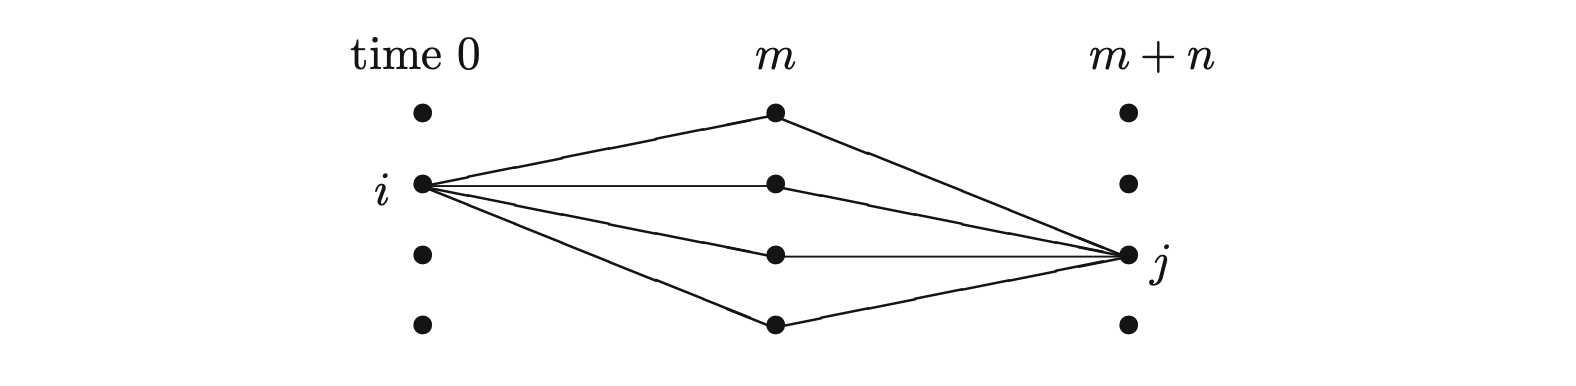
\includegraphics[width=0.9\textwidth]{figures/split_steps.png}
\end{figure}

\newpage
\subsection{多步转移概率与矩阵乘法}

\begin{definition}
    设 $X=\{X_n,n\geq 0\}$ 为马氏链, 称
    \[
    p_{ij}(m,m+n):=\PP(X_{n+m}=j|X_m=i)\quad (i,j\in S, m,n\geq 0)
    \]
    为 $X$ 的 $n$ 步转移概率, 并称 $P(m,m+n)=(p_{ij}(m,m+n))_{i,j\in S}$ 为 $X$ 的 $n$ 步转移(概率)矩阵, 其中
    \[
    p_{i,j}(0,0)=\delta_{ij}=\begin{cases}
        1 & i=j\\
        0 & i\neq j
    \end{cases}
    \]
\end{definition}

当 $X$ 时齐, $P(m,m+1)=(p_{ij}(m,m+1))_{i,j\in S}=(p_{ij}(0,1))_{i,j\in S}=(p_{ij})_{i,j\in S}$

可见 $n=1$ 时, $P(m,m+1)$ 与 $m$ 无关.那 $n>1$ 时呢?

\subsubsection{Chapman-Kolmogorov方程}

\begin{theorem}[C-K方程]\label{thm:CK}
    设 $\{X_n,x\geq 0\}$ 为马氏链
    \begin{equation}
p_{ij}(m,m+n+r)=\sum_{k\in S}p_{ik}(m,m+n)p_{kj}(m+n,m+n+r)
\label{eq:CK}
\end{equation}
    其中 $i,j\in S,m,n,r\geq 0$, 即
    \[
    P(m,m+n+r)=P(m,m+n)P(m+n,m+n+r)
    \]
\end{theorem}

\begin{figure}[H]
    \centering
    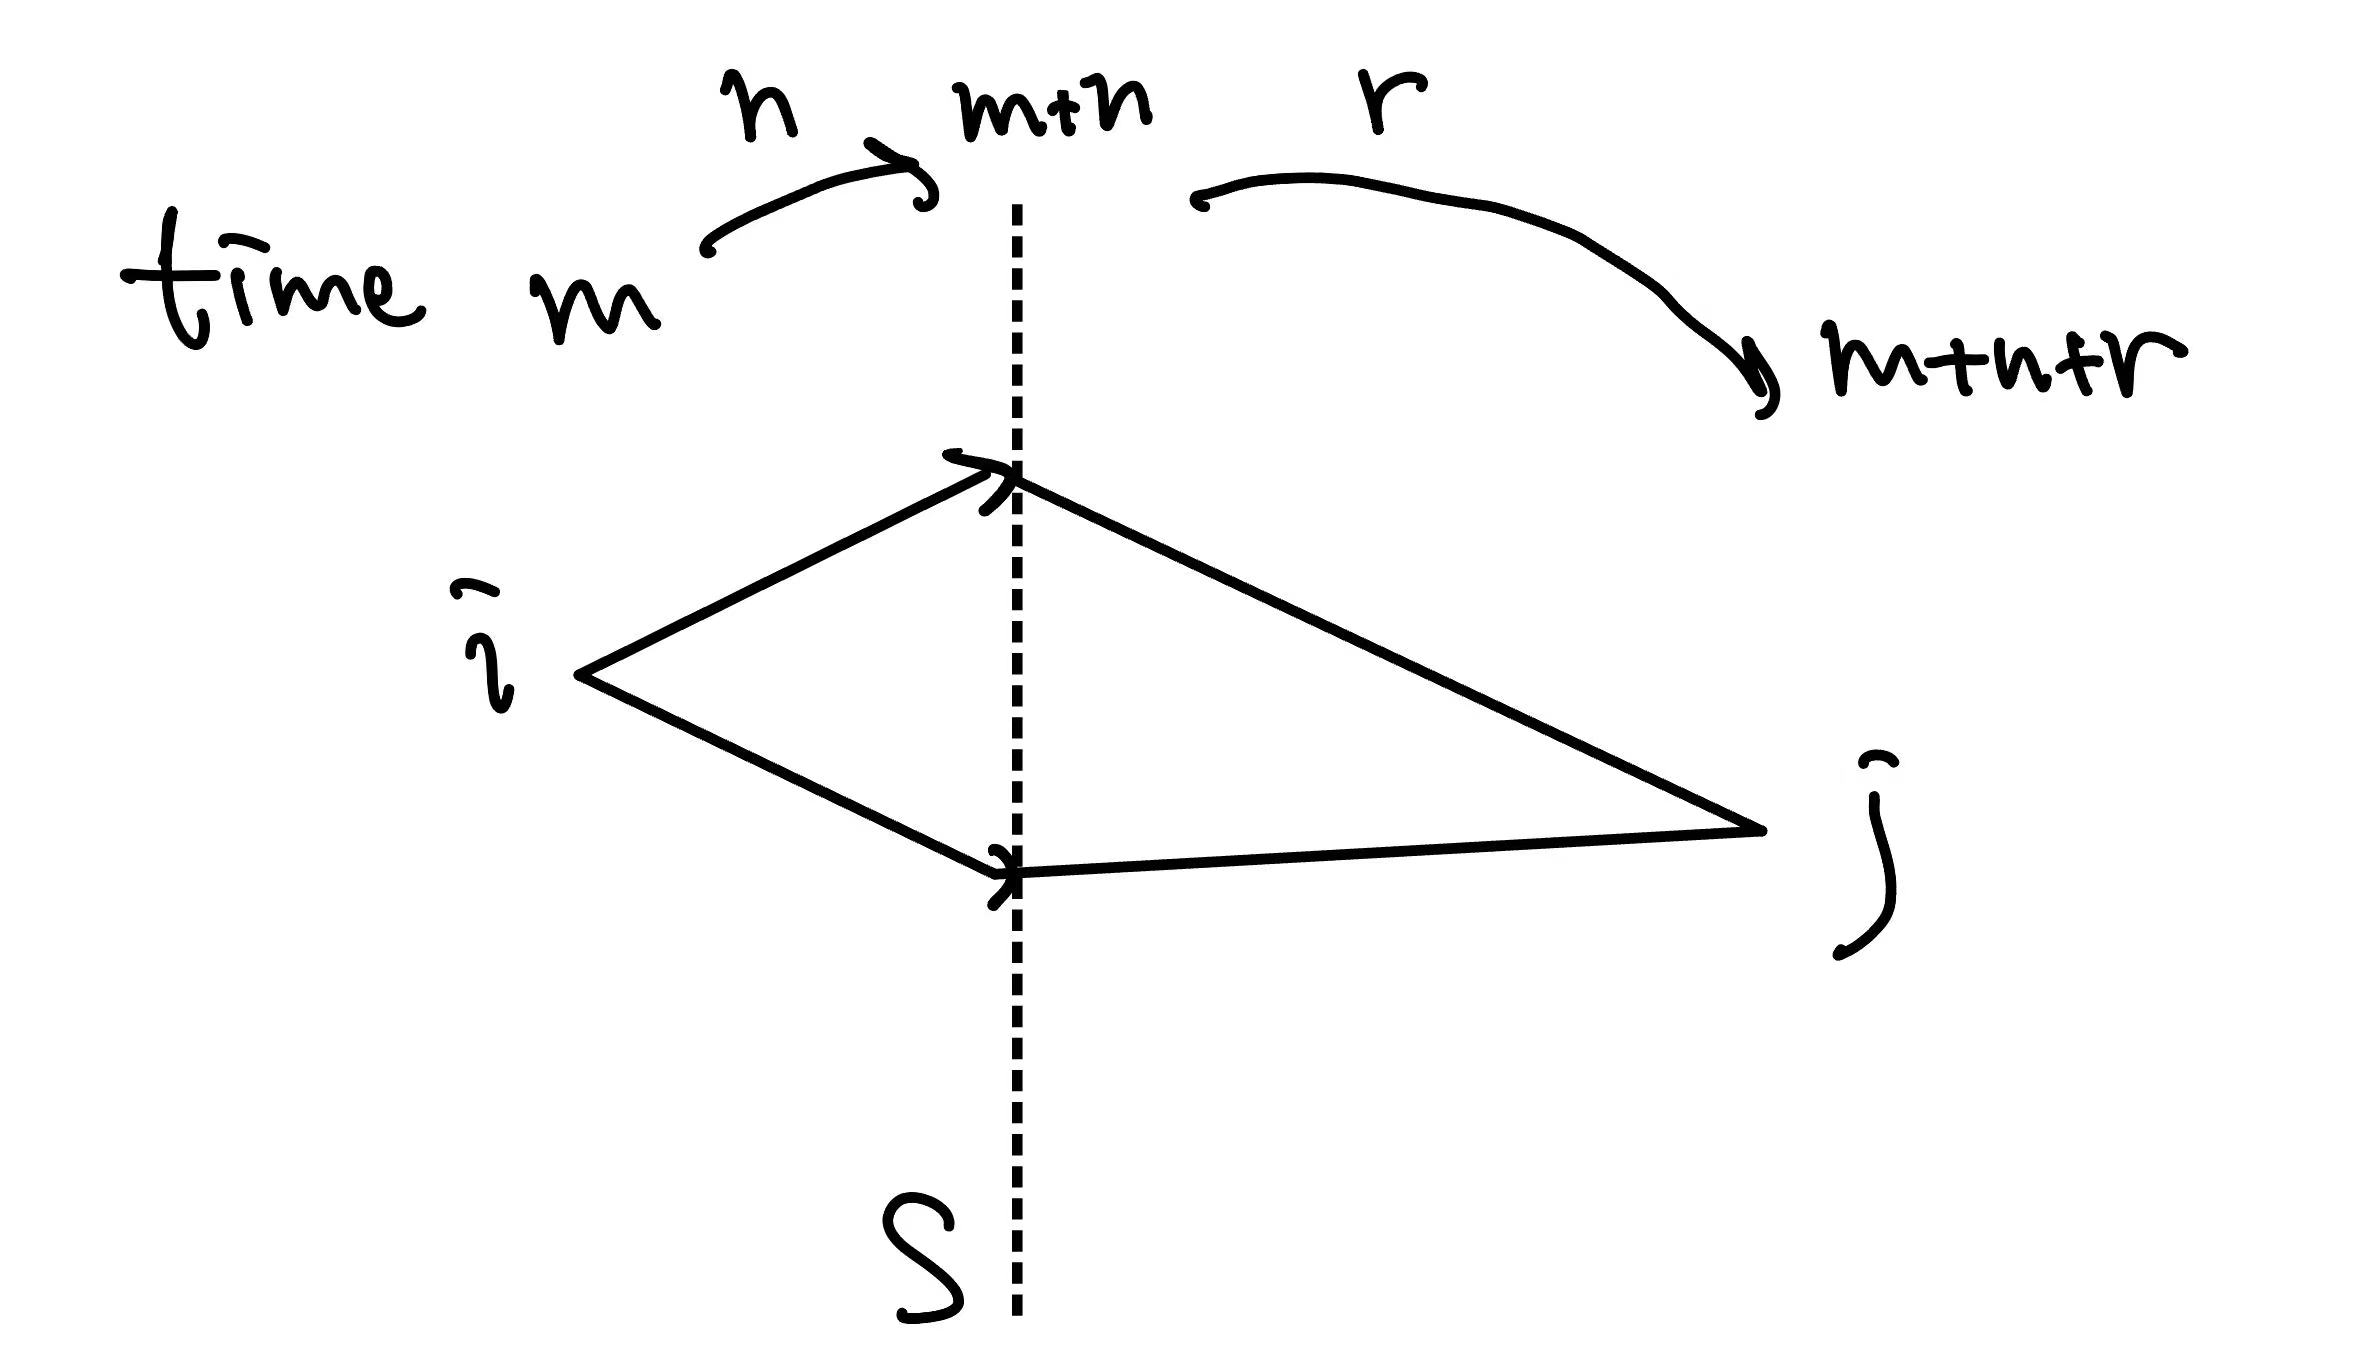
\includegraphics[width=0.55\textwidth]{figures/multi_steps.jpg}
    \caption{Multi-steps}
\end{figure}

证明:

\[
\begin{aligned}
    p_{ij}(m,m+n+r)&=P(X_{m+n+r}=j|X_m=i)\\
    &=\sum_{k\in S}P(X_{m+n+r}=j,X_{m+n}=k|X_m=i)\\
    &=\sum_{k\in S}\PP_{\{X_m=i\}}(X_{m+n+r}=j|X_{m+n}=k)\PP_{\{X_m=i\}}(X_{m+n}=k)\quad [\text{乘法公式}\eqref{eq:multiply_func}]\\
    &=\sum_{k\in S}p_{ik}(m,m+n)p_{kj}(m+n,m+n+r)\quad [\text{Markov}]
\end{aligned}
\]

\begin{corollary}
    设 $X$ 为具有(一步)转移矩阵 $P$ 的时齐马氏链, 则
    \begin{enumerate}
        \item $\forall m,n\geq 0$, 有 $P(m,m+n)=P(0,n)=P^n$.其中, 约定 $P^0=I$(单位矩阵)
        
        从而, 可记 $X$ 的 $n$ 步转移概率为 $p_{ij}(n)$ 或 $p_{ij}^{(n)}$, $n$ 步转移概率矩阵为 $P(n)$, 且有
        \[
        P(n)=P^n=(p_{ij}^{(n)})_{i,j\in S}
        \]
        \item C-K 方程可改写为
        \[
        p_{ij}(m+n)=\sum_{k\in S}p_{ik}^{(m)}p_{kj}^{(n)}
        \]
        $P(m+n)=P(m)P(n)$, 即 $P^{m+n}=P^m P^n$
    \end{enumerate}
\end{corollary}

证明:

\[
\begin{aligned}
    P(m,m+n)&=P(m,m+1)\cdot P(m+1,m+n)\quad [\text{C-K}]\\
    &=P\cdot P(m+1,m+n)\quad [\text{时齐}]\\
    &=P^n\qed
\end{aligned}
\]

\begin{proposition}
    $\forall n\geq 0, P(n)=P^n$ 仍是一个随机矩阵 (Theorem \ref{thm:random_matrix})
\end{proposition}

证明:$n=2$时, $P^2=(p_{ij}(2))_{i,j\in S}$

$\Rightarrow$
\[
\begin{aligned}
    \sum_{j\in S}p_{ij}(2)&=\sum_{j\in S}\sum_{k\in S}p_{ik}p_{kj}\quad [\text{C-K}, \text{ 默认}p_{ik}(1)=p_{ik}]\\
    &=\sum_{k\in S}\sum_{j\in S}p_{ik}p_{kj}\\
    &=\sum_{k\in S}p_{ik}\cdot(\sum_{j\in S}p_{kj})\\
    &=\sum_{k\in S}p_{ik}=1\qed
\end{aligned}
\]
第二个等号, 级数可交换是因为非负, 要么有限(收敛)、要么$+\infty$(发散)

\subsubsection{马氏链的任意有限维分布}

\begin{proposition}
    $X\sim\text{Markov}(\mu, P)$, 其中 $\mu=(\mu_i)_{i\in S}, P=(p_{ij})_{i,j\in S}$, 则
    \[
    \PP(X_{u_1}=i_1,\cdots,X_{u_n}=i_n)=\mu_{i_1}^{(u_1)}\prod_{k=1}^{n-1}p_{i_k,i_{k+1}}^{(u_{k+1}-u_k)}
    \]
    其中, $0<u_1<u_2<\cdots<u_n$, $i_1,i_2,\cdots,i_n\in S$, $\mu^{(u_1)}=(\mu_i^{(u_1)})_{i\in S}$ 为 $X_{u_1}$ 的有限维分布
\end{proposition}

证明:
\[
\begin{aligned}
    \PP(X_{u_1}=i_1,\cdots,X_{u_n}=i_n)&=\PP(X_{u_1}=i_1)\cdot \PP(X_{u_2}=i_2|X_{u_1}=i_1)\cdots \PP(X_{u_n}=i_n|X_{u_1}=i_1,\cdots,X_{u_{n-1}}=i_{n-1})\\
    &=(\mu_{i_1}^{(u_1)})p_{i_1,i_2}^{(u_2-u_1)}\cdots p_{i_{n-1},i_n}^{(u_n-u_{n-1})}\quad [\text{Markov}]\\
    &=\mu_{i_1}^{(u_1)}\prod_{k=1}^{n-1}p_{i_k,i_{k+1}}^{(u_{k+1}-u_k)}
\end{aligned}
\]

用概率表示不够直观, 尝试用转移矩阵来表示

\begin{lemma}
   $\mu^{(m+n)}=\mu^{(n)}P^m(\forall m,n\geq 0)$, 即
   \[
   \mu_j^{(m+n)}=(\mu^{(n)}P^m)_j=\sum_{i\in S}\mu_i^{(n)}p_{ij}^{(m)}
   \]
   特别地, 取 $n=0$, 则 $\mu^{(m)}=\mu\cdot P^m$($\mu$看成行向量), 即 $\mu_j^{(m)}=(\mu P^m)_j=\sum_{i\in S}\mu_i\cdot p_{ij}^{(m)}$
\end{lemma}

证明:
\[
\begin{aligned}
    \mu_j^{(n+m)}=\PP(X_{n+m}=j)&=\sum_{i\in S}\PP(X_{n+m}=j|X_n=i)\PP(X_n=i)\\
    &=\sum_{i\in S}p_{ij}(m)\mu_i^{(n)}\\
    &=(\mu^{(n)}P^m)_j\qed
\end{aligned}
\]

$\Rightarrow \mu^{(m+n)}=\mu^{(n)}P^m$

\begin{theorem}[任意有限维分布II]
    $\forall 0\leq u_1<u_2<\cdots<u_n, i_1,\cdots,i_n\in S$
    \[
    \PP(X_{u_1}=i_1,\cdots,X_{u_n}=i_n)=(\mu P^{u_1}_{i_1})\prod_{k=1}^{n-1}P_{i_k,i_{k+1}}^{u_{k+1}-u_k}
    \]
    其中, $P_{i,j}^m=:(P^m)_{i,j}=:p_{i,j}^{(m)}$
\end{theorem}

讨论随机过程地存在性:

抽象地, $\mu,P\xrightarrow{\text{Thm }\eqref{thm:Kolmogorov}}\text{有限维分布族}\rightarrow X\sim \text{Markov}(\mu,P)$, $\mu,P$可以刻画具备对称性、相容性的有限维分布

具体地, 参考Resnick\cite{resnick}, P62, Section 2.1

\newpage
\subsection{(从固定点出发的)马氏链}

固定 $i\in S$, 定义 $\PP_i(\cdot)=\PP(\cdot|X_0=i)$, $\EE_i(X)=\EE(X|X_0=i)=\sum_{x\in S}x\PP_i(X=x)$

\subsubsection{链的状态:常返和暂留}

\begin{definition}
    称状态 $i$ 为常返的, 若
    \[
    \PP_i(X_n=i\text{对某个}n\geq 1)=1
    \]
    如果上面的概率$<1$, 则称为暂留的/非常返的
    
    注:$i$ 常返 $\Leftrightarrow$ $\PP_i(\cup_{n\geq 1}\{X_n=i\})=1$
\end{definition}

思考:$i$ 常返 $\Leftrightarrow$ “不停地/无数次回到$i$”

$\qquad \Leftrightarrow$ $\PP_i(\omega|\omega\in \text{无数多个} \{X_n=i\})$

$\qquad \Leftrightarrow$ $\PP_i(\omega|\omega\in\cap_{k\geq 1}\cup_{n\geq k}\{X_n=i\},\forall k)$

$\qquad \Leftrightarrow$ $\PP_i(X_n=i, i.o.)$ (infinitely often)

无数多次返回 $i$ 可严格定义为:
\[
\bigcap_{k\geq 1}\bigcup_{n\geq k}\{X_n=i\}
\]
集合的语言中, $\cup$即$\exists$, $\cap$即$\forall$, 因此
\begin{itemize}
    \item $\bigcup_{n\geq k}\{X_n=i\}$ 表示 $\exists n_0\geq k$ 使得 $X_{n_0}=i$
    \item 对 $\forall k$ 取交集 $\bigcap_{k\geq 1}$, 即无论 $k$ 多大, 总存在更大的 $n$ 满足 $X_n=i$, 从而保证无限次返回
\end{itemize}
即 $\forall k, \exists n_k, \stt \{X_{n_k}=i\}$发生
\[
\begin{aligned}
    k=1&, n_1\geq k\\
    k=n_1+1&, n_2\geq n_1+1>n_1\\
    &\cdots
\end{aligned}
\]

\begin{remark}[如何进一步理解]
    无界和$\infty$的区别是什么?

无界:$\forall M>0,\exists k, \stt |x_k|>M$
\begin{example}
    $1,2,3,4,\cdots$ 为 $\infty$/无界

    $1,0,2,0,3,0,4,\cdots$ 并非 $\infty$, 但是无界的
\end{example}
迁移到$\bigcap_{k\geq 1}\bigcup_{n\geq k}$的例子
\begin{example}
    $A_1=\{0,1\},A_2=\{2\},A_3=\{0,3\},\cdots$, 则
    \[
    \bigcap_{k=1}^{\infty}\bigcup_{n\geq k}A_n=\{0\},\qquad \bigcap_{k=1}^{\infty}A_k=\emp
    \]
    其中 $\bigcap_{k=1}^{\infty}\bigcup_{n\geq k}$ 也即 $\limsup$
\end{example}
\end{remark}

但我们推理得到的“常返”和定义里的并不等价
\[
\bigcap_{k\geq 1}\bigcup_{n\geq k}\{X_n=i\}\nLeftrightarrow \bigcup_{n\geq 1}\{X_n=i\}
\]
且LHS是RHS的子集, 因此由定义的$\PP(RHS)=1$不能推出$\PP(LHS)=1$.于是我们疑惑为什么会叫它常返.这里要用到高阶知识“停时”, 我们最后会回到这个问题.

下面给出几种判断常返/暂留的方法.

\subsubsection{从数学角度:并改写成不交并}

$i$ 常返 $\Leftrightarrow$ $\PP_i(\cup_{n\geq 1}\{X_n=i\})=1$

$\qquad \Leftrightarrow \PP_i(\text{有限步到达}i)=1$

$\qquad \Leftrightarrow \PP(\text{从}i\text{出发条件下, 有限时间内回到}i)=1$

$B_1(i)=\{X_1=i\},B_2(i)=\{X_2=i\}\backslash \{X_1=i\}=\{X_2=i,X_1\neq i\},$ $\cdots,$ $B_n(i)=\{X_n=i,X_{n-1}\neq i\cdots,X_1\neq i\}$

由练习\ref{exer:disjoint_union}, 
\begin{equation}
\sum_{n\geq 1}B_n(i)=\bigcup_{n\geq 1}\{X_n=i\} 
\end{equation}
$i$ 常返 $\Leftrightarrow$ $1=\PP_i(\sum_{n\geq 1}B_n(i))=\sum_{n\geq 1}\PP_i(B_n(i))$, 第二个等号由可列可加性得到(定义\ref{def:prob_measure})
\[
\begin{aligned}
    \PP_i(B_n(j))=\PP_i(X_n=j,X_{n-1}\neq j,\cdots,X_1\neq j)&=\PP_i(\text{首次访问}j\text{的时刻为}n)\\
    &=\PP_i(\text{走}n\text{步首次到达}j)
\end{aligned}
\]
故
\[
\PP_i\left(\sum_{n\geq 1}B_n(j)\right)=\PP_i(\text{首次访问}j\text{的时刻为有限时间})=\PP_i(\text{有限时间内首次访问}j)
\]
记号
\begin{equation}
\begin{cases}
f_{ij}:=\PP_i\left(\sum_{n\geq 1}B_n(j)\right)=\sum_{n\geq 1}\PP_i(B_n(j))=\PP_i(\text{首次访问}j\text{的时刻为有限时间})\\
f_{ij}(n):=\PP_i(B_n(j))=\PP_i(\text{首次访问}j\text{的时刻为}n)
\end{cases}
\label{eq:def_f}
\end{equation}

\begin{proposition}
    (不交并视角下)常返和暂留的等价命题
    \begin{enumerate}
        \item $i$ 常返 $\iff$ 
        \begin{equation}
				1=f_{ii}=\sum_{n\geq 1}f_{ii}(n)
				\label{eq:recurrent_mathview}
				\end{equation}
        \item $i$ 暂留 $\iff$ 
        \begin{equation}
				1>f_{ii}=\sum_{n\geq 1}f_{ii}(n)
				\label{eq:transient_mathview}
				\end{equation}
    \end{enumerate}
\end{proposition}

证明:由可列可加性, $f_{ii}=\sum_{n\geq 1}f_{ii}(n)$总是成立.而$f_{ii}=\PP_i(\sum_{n\geq 1}B_n(i))=\PP_i(\cup_{n\geq 1}\{X_n=i\})$, 即$i$常返的定义, 因此 $f_{ii}=1$. 若$i$暂留, 则 $f_{ii}\neq 1$, 由概率测度的定义, $f_{ii}$不能大于1, 所以 $f_{ii}<1$.\qed

\subsubsection{从“多步转移概率”角度判别}

定义新记号($P$不是转移矩阵)
\[
P_{ij}(s):=\sum_{n\geq 0}s^n p_{ij}(n)\qquad F_{ij}(s):=\sum_{n\geq 0}s^n f_{ij}(n)
\]
其中, $p_{ij}(0)=\delta_{ij},f_{ij}(0)=0$
\[
\delta_{ij}=\begin{cases}
    1 & i=j\\
    0 & i\neq j
\end{cases}
\]

注:当 $|s|<1$ 时, $P_{ij}(s),F_{ij}(s)$ 绝对收敛

由 Abel 连续性定理, 
\[
\lim_{s\uparrow 1}F_{ij}(s)=\sum_{n\geq 1}f_{ij}(n)=f_{ij}\in [0,1]
\]
\[
\lim_{s\uparrow 1}P_{ij}(s)=\sum_{n\geq 0}p_{ij}(0)=\text{finite}/+\infty
\]
\begin{lemma}
    [Grimmett\cite{grimmett}, Thm 6.3.3] 设 $|s|<1$, 则
    \begin{equation}
    P_{ij}(s)=\delta_{ij}+P_{jj}(s)F_{ij}(s)
    \label{eq:genfunc}
    \end{equation}
    其中
    \[
    \delta_{ij}=\begin{cases}
        1 & i=j\\
        0 & i\neq j
    \end{cases}
    \]
\end{lemma}

证明:构造不交并, $B_m(i)=\{X_m=i,X_{m-1}\neq i,\cdots,X_1\neq i\}, m\geq 1$

$\sum_{m\geq 1}B_m(i)=\cup_{n\geq 1}\{X_n=i\}, B_m(i)\st \{X_n\neq i\}, m\geq n+1$
\begin{equation}
\begin{aligned}
    p_{ij}(n)=\PP_i(X_n=j)&=\PP_i(\{X_n=j\}\cap \sum_{m\geq 1}B_m(j))\\
    &=\sum_{m\geq 1}\PP_i(\{X_n=j\}\cap B_m(j))
    &=\sum_{m=1}^n\PP_i(\{X_n=j\}\cap B_m(j))
\end{aligned}
\label{eq:genfunc_eq1}
\end{equation}

最后一个等号成立是因为 $m\geq n+1$ 时 $\{X_n=j\}\cap B_m(j)$ 为空集
\begin{equation}
\sum_{m=1}^n\PP_i(\{X_n=j\}\cap B_m(j))=\sum_{m=1}^n\PP_i(X_n=j|B_m(j))\PP_i(B_m(j))
\label{eq:genfunc_eq2}
\end{equation}
其中 $X_m=j,X_{n-1}\neq j,\cdots,X_1\neq j$, $X_{n-1}\in S\backslash \{j\}$

用一般而非单点的马氏性\eqref{eq:markov_equiv_M3}
\begin{equation}
\begin{aligned}
    \sum_{m=1}^n\PP_i(X_n=j|B_m(j))\PP_i(B_m(j))&=\sum_{m=1}^n\PP(X_n=j|X_m=j)\cdot f_{ij}(m)\\
    &=\sum_{m=1}^n p_{jj}(n-m)\cdot f_{ij}(m)
\end{aligned}
\label{eq:genfunc_eq3}
\end{equation}

整合\eqref{eq:genfunc_eq1}, \eqref{eq:genfunc_eq2}, \eqref{eq:genfunc_eq3},
\begin{equation}
p_{ij}(n)=\sum_{m=1}^n p_{jj}(n-m)\cdot f_{ij}(m)
\label{eq:genfunc_eq4}
\end{equation}

当 $n\geq 1$ 时, 
\[
\begin{aligned}
    P_{ij}(s)&=s^0p_{ij}(0)+\sum_{n\geq 1}s^n\cdot p_{ij}(n)\\
    &=\delta_{ij}+\sum_{n\geq 1}s^n\sum_{m=1}^n p_{jj}(n-m)f_{ij}(m)\\
    &=\delta_{ij}+\sum_{n\geq 1}\sum_{m=1}^n s^n p_{jj}(n-m)f_{ij}(m)\\
    &=\delta_{ij}+\sum_{n\geq 1}\sum_{m=1}^n(s^{n-m}p_{jj}(n-m))(s^m f_{ij}(m))\\
    &=\delta_{ij}+\sum_{n=1}^{\infty}\sum_{m=1}^{\infty}\II_{\{1\leq m\leq n\}}(s^{n-m}p_{jj}(n-m))(s^m f_{ij}(m))
\end{aligned}
\]
【重要技巧】把 $\II_{\{1\leq m\leq n\}}(s^{n-m}p_{jj}(n-m))(s^m f_{ij}(m))$ 看作 $a_{n,m}$, 由Lemma \ref{lem:abs_convergence}考察绝对收敛

$0\leq s<1, |s|=s$

正向级数一定有意义, 就看是有限/$\infty$
\[
\begin{aligned}
    &\sum_{n=1}^{\infty}\sum_{m=1}^{\infty}\II_{\{1\leq m\leq n\}}s^{n-m}p_{jj}(n-m)s^m f_{ij}(m)\\
    =&\sum_{m=1}^{\infty}\sum_{n=1}^{\infty}\II_{\{1\leq m\leq n\}}s^{n-m}p_{jj}(n-m)s^m f_{ij}(m)\\
    =&\sum_{m=1}^{\infty}(\sum_{n=m}^{\infty}s^{n-m}p_{jj}(n-m))s^m f_{ij}(m)\\
    =&(\sum_{k=0}^{\infty}s^{k}p_{jj}(k))(\sum_{m=1}^{\infty}s^m f_{ij}(m))<\infty
\end{aligned}
\]
其中 $k=n-m$. 因为 $s^0f_{ij}(0)=0$, 则 $\sum_{m=0}^{\infty}s^m f_{ij}(m)=\sum_{m=1}^{\infty}s^m f_{ij}(m)$.代回原式
\[
P_{ij}(s)=\delta_{ij}+P_{jj}(s)\cdot F_{ij}(s)
\]

\begin{proposition}\label{prop:states_equiv}
(多步转移概率视角下)常返和暂留的等价命题
\begin{enumerate}
\item $j$ 常返 $\iff$
\begin{equation}
1=f_{jj}\Leftrightarrow \sum_{n\geq 0}p_{jj}(n)=\infty
\label{eq:recurrent_multistep}
\end{equation}
\item $j$ 暂留 $\iff$
\begin{equation}
\begin{aligned}
1>f_{jj}&\Leftrightarrow \sum_{n\geq 0}p_{jj}(n)<\infty\\
&\Rightarrow \sum_{n\geq 0}p_{ij}(n)<\infty, \forall i\in S\\
&\Rightarrow \limit{n}p_{ij}(n)=0,\forall i\in S
\end{aligned}
\label{eq:transient_multistep}
\end{equation}
\end{enumerate}
\end{proposition}

证明:只证(1). $|s|<1$时, $P_{ij}(s)=\delta_{ij}+P_{jj}(s)F_{ij}(s)$

令$i=j$, $P_{jj}(s)=1+P_{jj}(s)F_{jj}(s)$

\begin{equation}
P_{jj}(s)=\frac{1}{1-F_{jj}(s)}
\label{eq:genfunc_special}
\end{equation}

由\eqref{eq:recurrent_mathview}, $j$ 常返 $\iff$ $1=f_{jj}=F_{jj}(1)\overset{\text{Abel}}{=}\lim_{s\uparrow 1}F_{jj}(s)$

对\eqref{eq:genfunc_special}, 令 $s\to 1$, 有 $\sum_{n\geq 0}p_{jj}(n)=+\infty$\qed

\begin{problem}[作业5-1]
证明:$j$ 暂留 $\Rightarrow \sum_{n\geq 0}p_{ij}(n)<\infty, \forall i\in S$
\end{problem}
\begin{proof}
由\eqref{eq:genfunc}, 若 $s\uparrow 1$, 
\[
\sum_{n\geq 0}p_{ij}(n)=\delta_{ij}+\left(\sum_{n\geq 0}p_{jj}(n)\right)\left(\sum_{n\geq 0}f_{ij}(n)\right)\leq \delta_{ij}+\sum_{n\geq 0}p_{jj}(n)<\infty
\]
其中 $\sum_{n\geq 0}f_{ij}(n)=f_{ij}\in [0,1]$.
\end{proof}

\subsubsection{从“首次回访时间”角度判别}
\[
\begin{aligned}
    j\text{常返}\iff& 1=\PP_j(X_n=j\text{ 对某个}n\geq 1)=\PP_j(\text{有限时间内回访}j)\\
    \iff& 1=f_{jj}=\PP_j(\underbrace{\text{首次回访}j\text{的时刻}}_{T_j<\infty}\text{有限})\\
    & 1=\sum_{n\geq 1}f_{jj}(n)=\sum_{n\geq 1}\PP_j(\underbrace{\text{首次回访}j\text{的时刻}}_{T_j=n}\text{是}n)
\end{aligned}
\]
\begin{definition}[首次回访时间]
    首次回访$j$的时刻
    \begin{equation}
T_j=\min\{n\geq 1|X_n=j\}
\label{eq:def_revisit_time}
\end{equation}
    约定 $\min \emp=+\infty$
\end{definition}

注:$\{T_j=\infty\}\iff \{\omega|\{n\geq 1|X_n(\omega)=j\}=\emp\}\iff \{\omega|X_n(\omega)\neq j,\forall n\geq 1\}=\cap_{n\geq 1}\{X_n\neq j\}$

$\{T_j<\infty\}=(\{T_j=\infty\})^c=(\cap_{n\geq 1}\{X_n\neq j\})^c=\cup_{n\geq 1}(\{X_n\neq j\})^c=\cup_{n\geq 1}\{X_n=j\}$

这个式子串联起常返的定义和$T_j$的关系, 于是有以下性质.

\begin{property}
    $f_{jj}=\PP_j(T_j<\infty), f_{jj}(n)=\PP_j(T_j=n)$
\end{property}

由\eqref{eq:def_f}知, $f_{ij}, f_{ij}(n)$ 是由不交并定义的, 对于“首次回访时间”这一角度, 定义新的符号
\begin{equation}
\rho_{ij}:=\PP_i(T_j<\infty)
\label{eq:def_rho}
\end{equation}

\begin{proposition}
(首次回访时间视角下)常返和暂留的等价命题 
    \begin{enumerate}
        \item $j$ 常返 $\iff$ 
        \begin{equation}
1=\rho_{jj}=\PP_j(T_j<\infty)\iff 0=\PP_j(T_j=\infty)
\label{eq:recurrent_revisit}
\end{equation}
        \item $j$ 暂留 $\iff$ 
        \begin{equation}
1>\rho_{jj}=\PP_j(T_j<\infty)\iff 0<\PP_j(T_j=\infty)
\label{eq:transient_revisit}
\end{equation}
    \end{enumerate}
\end{proposition}

证明:由\eqref{eq:recurrent_multistep}, \eqref{eq:transient_multistep}, $j\text{常返}\iff 1=f_{jj}=\rho_{jj}\iff 0=1-\rho_{jj}$, 其余同理.\qed

\begin{definition}[平均回访时间]
    $j$ 的平均回访时间
    \begin{equation}
m_j:=\EE_jT_j=\EE(T_j|X_0=j)
\label{eq:def_avg_revisit_time}
\end{equation}
\end{definition}

\begin{theorem}
用不交并表示平均回访时间.
\begin{equation}
m_j=\EE_j T_j=\begin{cases}
\sum_{n\geq 1}nf_{jj}(n) & j\text{常返}\\
\infty & j\text{暂留}
\end{cases}
\label{eq:avg_revisit_time}
\end{equation}
\end{theorem}

证明:

(1) $j$暂留 $\Rightarrow$ $\PP_j(T_j=\infty)>0$

$T_j=T_j\II_{\{T_j=\infty\}}+T_j\II_{\{T_j<\infty\}}$

$\EE_j T_j=\EE_j T_j\II_{\{T_j=\infty\}}+\EE_j T_j\II_{\{T_j<\infty\}}\geq \EE_j T_j\II_{\{T_j=\infty\}}=\infty\cdot \PP_j(T_j=\infty)=\infty$

(2) $j$常返 $\Rightarrow$ $\PP_j(T_j=\infty)=0$

取期望时不起作用, 因为 $0\cdot \infty$ 是不定形
\[
\EE_j T_j=\EE_j T_j\II_{\{T_j<\infty\}}=\EE_j T_j\II_{\sum_{n\geq 1}\{T_j=n\}}\overset{\eqref{eq:def_drv}}{=}\EE_j\sum_{n\geq 1}T_j\II_{\{T_j=n\}}=\sum_{n\geq 1}n\PP_j(T_j=n)=\sum_{n\geq 1}n f_{jj}(n)
\]
\begin{definition}[正常返/零常返]\label{def:recurrent_types}
    $j$常返时
    \begin{enumerate}
        \item $\EE_j T_j<\infty$ 称$j$是正常返
        \item $\EE_j T_j=\infty$ 称$j$是零常返(平均意义上再也不回来)
    \end{enumerate}
\end{definition}

$j$ 常返 $\iff 1=f_{jj}\iff \sum_{n\geq 0}p_{jj}(n)=\infty$

$\iff 1=\rho_{jj}=\PP_j(T_j<\infty)\iff 0=\PP_j(T_j=\infty)$
\begin{equation}
\begin{aligned}
\PP_j(T_j<\infty)&=\PP(\text{从}j\text{出发条件下, 首次回到}j\text{的时刻有限})\\
&=\PP(\text{从}j\text{出发条件下, 有限时间内至少访问}j\text{有1次})\\
&=\PP(\text{从}j\text{出发条件下, 有限时间内回访}j\text{的次数}\geq 1)
\end{aligned}
\label{eq:time&counts}
\end{equation}

\begin{definition}[访问次数]
    链在时刻$0$之后, 访问$j$的次数
    \begin{equation}
N(j):=\# \{n\geq 1|X_n=j\}=\sum_{n\geq 1}\II_{\{X_n=j\}}
\label{eq:def_counts}
\end{equation}
\end{definition}

注:$N(j):\Omega\to \{0,1,2,\cdots\}\cup \{+\infty\}$

至此, 我们已经从四个角度表示了常返
\begin{enumerate}
\item 常返的定义
\item 不交并
\item 多步转移概率
\item 首次访问时间
\end{enumerate}
做个阶段性小结, 回顾 $i$ 常返的几种等价表示
\[
\begin{aligned}
    i\text{常返} &\overset{\text{Def}}{\iff}1=\PP_i(\bigcup_{n\geq 1}\{X_n=i\})\\
    &\iff 1=f_{ii}:=\sum_{n\geq 1}f_{ii}(n)=\sum_{n\geq 1}\PP_i(X_1\neq i,\cdots, X_{n-1}\neq i,X_n=i)\\
    &\iff \sum_{n\geq 1}p_{ii}(n)=\infty\\
    &\iff 1=\rho_{ii}=\PP_i(T_i^{(1)}:=T_i<\infty)
\end{aligned}
\]
由\eqref{eq:time&counts}, $\PP_i(T_i<\infty)=\PP_i(N(i)\geq 1)$, 因此可得“回访次数”视角下 $i$ 常返的条件
\begin{proposition}
(回访次数视角下)常返和暂留的等价命题
\begin{enumerate}
\item $i$常返 $\iff$
\begin{equation}
\PP_i\{N(i)\geq 1\}=1
\label{eq:recurrent_count}
\end{equation}
\item $i$暂留 $\iff$ 
\begin{equation}
\PP_i\{N(i)\geq 1\}<1
\label{eq:transient_count}
\end{equation}
\end{enumerate}
\end{proposition}

另一方面, 我们从“常返”的文字含义推理.

无数次地回访 $\leftrightarrow$ 访问次数$=\infty$ $\leftrightarrow$
\[
\PP_i(N(i)=\infty)=1
\]
两种表述的等价条件互相等价吗?即
\[
\PP_i(N(i)\geq 1)\overset{?}{\iff} \PP_i(N(i)=\infty)
\]
需要 Strong Markov Property (SMP) 使上面$\Leftrightarrow$成立.这里先补充一些关于 $N(j)$ 的内容, 然后再回到证明.

考察 $\{N(y)=\infty\}=\cap_{k\geq 1}\{N(y)\geq k\}$

由概率测度的连续性(性质\ref{prt:measure_continuity})
\[
    \PP_x(N(y)=\infty)=\limit{k}\PP_x(N(y)\geq k)
\]
其中, 
\[
\begin{aligned}
    \PP_x(N(y)\geq k) &= \PP(\text{从}x\text{出发条件下, 访问}y\text{的次数}\geq k)\\
    &=\PP(\text{从}x\text{出发条件下, 至少访问}y\text{有}k\text{次})\\
    &=\PP(\text{从}x\text{出发条件下, 第}k\text{次访问}y\text{的时刻有限})
\end{aligned}
\]

\begin{definition}[第$k$次访问时间]
由 $T_y^{(1)}:=T_y:=\min\{n\geq 1|X_n=y\}, T_y^{(2)}:=\min\{n>T_y^{(1)}|X_n=y\}, \cdots$, 得到
\begin{equation}
T_y^{(k)}:=\min\{n>T_y^{(k-1)}|X_n=y\}, \quad \forall k\geq 2
\label{eq:revisit_k}
\end{equation}
\end{definition}

\begin{claim}
$N(y)\geq k$ 与“第 $k$ 次访问 $y$ 的时刻有限”等价, 
\begin{equation}
\PP_x(N(y)\geq k)=\PP_x(T_y^{(k)}<\infty)
\label{eq:time&count_k}
\end{equation}
\end{claim}

\begin{definition}
    (1) 第$k$次访问概率
    \begin{equation}
\rho_{xy}^{(k)}:=\PP_x(T_y^{(k)}<\infty)
\label{eq:prob_visit_k}
\end{equation}
    其中, $\rho_{xy}^{(1)}=\rho_{xy}$, rf.\eqref{eq:def_rho}
    
    (2) 第$k$次回访概率
    \begin{equation}
    \rho_{yy}^{(k)}:=\PP_y(T_y^{(k)}<\infty)
    \label{eq:prob_revisit_k}
\end{equation}
\end{definition}

注:$\rho_{yy}^{(2)}\overset{?}{=}\rho_{yy}\cdot \rho_{yy}$

直观上是这样, 但严格证明要求SMP

这是因为不同时间对应的是不同的随机过程, 如
\begin{itemize}
    \item $t=0$时, 过程是$\{X_n,n\geq 0\}$
    \item $t=T_j$时, 过程是$\{X_{T_j+n},n\geq 0\}$
\end{itemize}
SMP是一个使得 $X_{T_j+n}=X_n,\forall T_j$ 的性质, 之后会详细说.以上结论可总结成下面引理.

\begin{lemma}
    (由SMP知) $\rho_{xy}^{(k)}=\rho_{xy}\rho_{yy}^{(k-1)}$. 特别地, $\rho_{yy}^{(k)}=\rho_{yy}^k$
\end{lemma}

接着我们回到证明
\begin{equation}
\PP_i(N(i)\geq 1)=1 \iff \PP_i(N(i)=\infty)=1
\label{eq:equiv_count}
\end{equation}
证明:$\Leftarrow$ 显然, 因为 $\{N(i)=\infty\}$ 相对 $N(i)\geq 1$ 是小集合

$\Rightarrow$ 由于 $\{N(i)=\infty\}=\cap_{k\geq 1}\{N(i)\geq k\}$, $\{N(i)\geq k\}$ 单调下降, 所以 $\cap_{k\geq 1}\{N(i)\geq k\}=\lim_{k\to\infty}\{N(i)\geq k\}$.
\[
\PP_i(N(i)=\infty)=\limit{k}\PP_i(N(i)\geq k)\overset{\text{SMP}}{=}\limit{k}\rho_{ii}^k=1
\]
暂留的证明同理:
\[
\begin{aligned}
    i\text{暂留}&\iff 1> \rho_{ii}\\
    &\iff \PP_i(N(i)=\infty)=\limit{k}\rho_{ii}^k=0
\end{aligned}
\]

\subsubsection{从“平均回访次数”角度判别}
回顾\eqref{eq:def_counts},
\[
N(y)=\sum_{n\geq 1}\II_{\{X_n=y\}}=\sum_{k\geq 1}\II_{\{N(y)\geq k\}}
\]
\begin{lemma}[Durrett\cite{durrett}, lem 1.11]
    \begin{equation}
    \EE_yN(y)=\begin{cases}
        \infty & y\text{常返}\\
        \displaystyle\frac{\rho_{yy}}{1-\rho_{yy}} & y\text{暂留}
    \end{cases}
    \label{eq:lemma1.11}
    \end{equation}
\end{lemma}

证明:
\[
\EE_yN(y)=\EE_y\sum_{k\geq 1}\II_{\{N(y)\geq k\}}\overset{\text{Exa\eqref{exa:expec2prob}}}{=}\sum_{k\geq 1}\PP_y(N(y)\geq k)=\sum_{k\geq 1}\PP_y(T_y^{(k)}<\infty)=\sum_{k\geq 1}\rho_{yy}^{(k)}\overset{\text{SMP}}{=}\sum_{k\geq 1}\rho_{yy}^k
\]
$\rho_{yy}=1\Rightarrow \EE_yN(y)=\infty$

$\rho_{yy}<1\Rightarrow \EE_yN(y)=\rho_{yy}/(1-\rho_{yy})$\qed

\begin{proposition}
(平均回访次数视角下)常返和暂留的等价命题
\begin{enumerate}
\item $i$常返 $\iff$
\begin{equation}
\EE_i N(i)=\infty
\label{eq:recurrent_avg_count}
\end{equation}
\item $i$暂留 $\iff$
\begin{equation}
\EE_i N(i)<\infty
\label{eq:transient_avg_count}
\end{equation}
\end{enumerate}
\end{proposition}

证明(1):$\Rightarrow$ 由\eqref{eq:lemma1.11}, 显然

$\Leftarrow$ $N(y)$ 为非负r.v., 有当$k\to\infty$时, $\forall \omega, \sum_{n=1}^k\II_{\{X_n=y\}}(\omega)\uparrow \sum_{n=1}^{\infty}\II_{\{X_n=y\}}(\omega)$
\[
\EE_yN(y):=\limit{k}\EE_y\sum_{n=1}^k\II_{\{X_n=y\}}=\limit{k}\sum_{n=1}^k\EE_y\II_{\{X_n=y\}}=\limit{k}\sum_{n=1}^k\PP_y(X_n=y)=\sum_{n=1}^{\infty}p_{yy}(n)=\infty
\]
由\eqref{eq:recurrent_multistep}, $y$ 常返\qed

将上面几个角度总结成下面定理
\begin{theorem}[链的状态:等价表述]\label{thm:states_equiv}
\[
\begin{aligned}
    i\text{常返} &\overset{\text{Def}}{\iff}1=\PP_i(\bigcup_{n\geq 1}\{X_n=i\})\quad [\text{回访发生的概率}]\\
    &\iff 1=f_{ii}:=\sum_{n\geq 1}f_{ii}(n)=\sum_{n\geq 1}\PP_i(X_1\neq i,\cdots, X_{n-1}\neq i,X_n=i)\\
    &\iff \sum_{n\geq 1}p_{ii}(n)=\infty\\
    &\iff 1=\rho_{ii}=\PP_i(T_i^{(1)}:=T_i<\infty)=\PP_i\{N(i)\geq 1\}=1\\
    &\overset{\text{why the name}}{\iff} \PP_i(N(i)=\infty)=\limit{k}\PP_i(N(i)\geq k)\overset{\text{SMP}}{=}\limit{k}\rho_{ii}^k=1\\
    &\iff \EE_i N(i)=\infty
\end{aligned}
\]
\end{theorem}

\subsubsection{停时与强马氏性}

\begin{definition}[停时/Stopping time]
    随机变量 $\tau:\Omega\to \{0,1,2,\cdots\}\cup\{+\infty\}$, 满足 $\forall \infty>n\geq 0, \{\tau=n\}\in \sigma(X_0,\cdots,X_n)$, 称 $\tau$ 是关于 $(X_n)_{n\geq 0}$ 的停时
\end{definition}

\begin{example}
首次回访时刻是一个停时 $T_y^{(1)}:=T_y:=\min\{n\geq 1|X_n=y\}$.
    \[
    \begin{aligned}
        \{T_y^{(1)}=n\} &=\{X_1\neq y,\cdots,X_{n-1}\neq y,X_n=y\}\quad n\geq 1\\
        &=\{(X_0,X_1,\cdots,X_n)\in S\times(S\backslash \{y\})\times\cdots\times(S\backslash \{y\})\times \{y\}\}\\
        &\in \sigma(X_0,\cdots,X_n)=(X_0,\cdots,X_n)^{-1}(\bigotimes_{n+1}2^S)
    \end{aligned}
    \]
\end{example}

\begin{definition}[停止$\sigma$代数]
    $\tau$是关于 $(X_n)_{n\geq 0}$ 的停时, 定义
    \[
    \CF_{\tau}:=\{A|A\cap\{\tau=n\}\in\sigma(X_0,\cdots,X_n),\forall n\}
    \]
\end{definition}

注:$B\in \CF_{\tau}\Leftrightarrow B$是由$X_0,\cdots,X_{\tau}$决定的事件(这是直观上的解释, 因为$\tau$是随机的, 我们不知道“$\cdots$”是什么)$ \Leftrightarrow B\cap\{T=n\}\in \sigma(X_0,\cdots,X_n),\forall n$

停止 $\sigma$-代数的定义是为了形式化“到随机时间 $\tau$ 为止的信息”.因为 $\tau$ 本身是随机的, 我们不能直接写 $\sigma(X_0,\cdots,X_{\tau})$(因为 $\tau$ 不确定), 所以需要通过对所有可能的 $\tau=n$ 进行分解.

\begin{problem}[作业5-2]
设 $\tau$ 为关于 $(X_n)_{n\geq 0}$ 的停时, 即对任意的 $\infty>n\geq 0$, 有
\[
\{\tau=n\}\in\sigma(X_0,\cdots,X_n)
\]
证明:
\begin{enumerate}
\item (停止$\sigma$代数的定义) $\CF_{\tau}:=\{A|A\cap \{\tau=n\}\in \sigma(X_0,\cdots,X_n),\forall n\geq 1\}$ 是一个$\sigma$-代数
\item $\sigma(X_{\tau})\in \CF_{\tau}$
\end{enumerate}
\end{problem}

以下内容来自强马氏性讲义\cite{handout_SMP}.

\begin{lemma}[马氏性的小推广]\label{lem:markov_extend}
若 \( X \) 为马氏链, 则对任意 \( n,m \geq 0, x_n \in S, A \in \otimes_{n+1}2^S, B \in \otimes_{m+1}2^S \)(即 \( A \subset S^{n+1}, B \subset S^{m+1} \)), 有
\begin{equation}
\begin{aligned}
&\PP_{\{X_n=x_n\}}((X_0, \cdots , X_n) \in A, (X_n, \cdots , X_{n+m}) \in B)\\
=&\PP_{\{X_n=x_n\}}((X_0, \cdots , X_n) \in A) \times \PP_{\{X_n=x_n\}}((X_n, \cdots , X_{n+m}) \in B)
\end{aligned}
\label{eq:markov_extend}
\end{equation}
即 \((X_0, \cdots , X_n) \perp \!\!\! \perp_{\{X_n=x_n\}} (X_n, \cdots , X_{n+m})\) 的定义, rf.\eqref{eq:con_indep}
\end{lemma}

证明:回顾马氏性, rf.\eqref{eq:markov_equiv_condition_M2}

不妨设 \( A = A_0 \times \cdots \times A_n, B = B_n \times \cdots \times B_{n+m} \)

(Case 1) 若 \( x_n \notin A_n \) 或 \( x_n \notin B_n \), 则
\[
\PP_{\{X_n=x_n\}}((X_0, \cdots , X_n) \in A) = 0 \text{ 或 } \PP_{\{X_n=x_n\}}((X_n, \cdots , X_{n+m}) \in B) = 0
\]
且
\[
\PP_{\{X_n=x_n\}}((X_0, \cdots , X_n) \in A, (X_n, \cdots , X_{n+m}) \in B) = 0
\]
从而, \eqref{eq:markov_extend} 得证

(Case 2) 设 \( x_n \in A_n \), 且 \( x_n \in B_n \).若 \( n = 0, m = 0 \), 则显然有
\[
\PP_{\{X_n=x_n\}}((X_0, \cdots , X_n) \in A) = \PP_{\{X_n=x_n\}}((X_n, \cdots , X_{n+m}) \in B) = 1
\]
\[
\PP_{\{X_n=x_n\}}((X_0, \cdots , X_n) \in A, (X_n, \cdots , X_{n+m}) \in B) = 1
\]
此时, 显然有 \eqref{eq:markov_extend} 成立.若 \( n \geq 1, m \geq 1 \), 则
\[
\PP_{\{X_n=x_n\}}((X_0, \cdots , X_n) \in A) = \PP_{\{X_n=x_n\}} \left\{ X_j \in A_j, 0 \leq j \leq n-1 \right\}
\]
\[
\PP_{\{X_n=x_n\}}((X_n, \cdots , X_{n+m}) \in B) = \PP_{\{X_n=x_n\}} \left\{ X_j \in B_j, n+1 \leq j \leq n+m \right\}
\]
且
\[
\begin{aligned}
&\PP_{\{X_n=x_n\}}((X_0, \cdots , X_n) \in A, (X_n, \cdots , X_{n+m}) \in B)\\ =& \PP_{\{X_n=x_n\}} \left\{ X_j \in A_j, 0 \leq j \leq n-1, X_k \in B_k, n+1 \leq k \leq n+m \right\}\\
\overset{\eqref{eq:markov_equiv_condition_M2}}{=}& \PP_{\{X_n=x_n\}} \left\{ X_j \in A_j, 0 \leq j \leq n-1 \right\} \PP_{\{X_n=x_n\}} \left\{ X_k \in B_k, n+1 \leq k \leq n+m \right\}
\end{aligned}
\]
故而 \eqref{eq:markov_extend} 得证.对于其他情形 \( n \geq 1, m = 0 \) 或 \( n = 0, m \geq 1 \), 可类似证明.\qed

\begin{proposition}[强马氏性]
    $X:=\{X_n,n\geq 0\}\sim \text{Markov}(\mu,P)$, $\tau$是关于$(X_n)_{n\geq 0}$的停时, 则
    \begin{enumerate}
        \item 在$\{\tau<\infty\}$和$\{X_{\tau}=x\}$条件下
        \[
        (X_{\tau+n})_{n\geq 0}\sim\text{Markov}(\delta_x,P)
        \]
        其中 $\delta_x=(\delta_{xy})_{y\in S}$, 记号
        \[
        \delta_{xy}=\begin{cases}
            1 & y=x\\
            0 & y\neq x
        \end{cases}
        \]
        注:$(X_{\tau+n})_{n\geq 0}\sim \text{Markov}(\delta_x,P)$ under $\PP(\cdot|\tau<\infty,X_{\tau}=x)$.在原先的概率测度 $\PP$ 下,  $(X_{\tau+n})_{n\geq 0}$ 不是马氏链
        \item $\forall J\st \NN_0, \#J<\infty$, 有
        \[
        \sigma(X_{\tau+n},n\in J)\ind_{\{\tau<\infty,X_{\tau}=x\}}\CF_{\tau}
        \]
        注:\begin{enumerate}
            \item $(X_{\tau+n})_{n\geq 0}$与$X_0,\cdots,X_{\tau}$独立
            \item $(X_{\tau+n})_{n\geq 0}\ind \CF_{\tau}$ under $\PP(\cdot|\tau<\infty,X_{\tau}=x)$
        \end{enumerate}
    \end{enumerate}
\end{proposition}

证明:(1) 回顾马氏链的有限维分布, rf.\eqref{eq:markov_dist}, 

根据此结论, 我们只需考察链 \(\{X_{\tau + n}, n \geq 0\}\) 的有限维分布.

(Step 1) 设 \(j_0 \neq x\).则对任意的 \(n \geq 1, m \geq 0\), 有
\[
\PP(X_{\tau + 0} = j_0, \cdots, X_{\tau + n} = j_n, \tau = m, X_\tau = x) = 0
\]
关于 \(m \geq 0\) 求和, 并注意到 \(\{\tau < \infty\} = \sum_{m=0}^{\infty} \{\tau = m\}\), 得:
\[
\PP(X_{\tau + 0} = j_0, \cdots, X_{\tau + n} = j_n, \tau < \infty, X_\tau = x) = 0
\]
两边同除 \(P(\tau < \infty, X_\tau = x)\), 有
\[
\PP(X_{\tau + 0} = j_0, \cdots, X_{\tau + n} = j_n | \tau < \infty, X_\tau = x) = 0 = \delta_{x j_0} \prod_{k=0}^{n-1} p_{j_k j_{k+1}}
\]

(Step 2) 设 \(j_0 = x\).注意到, 对任意的 \(m \geq 0\), 有
\[
\{\tau = m\} \in \sigma(X_0, \cdots, X_m)
\]
故而, 由\eqref{eq:markov_extend}: 对任意的 \(n \geq 1, m \geq 0\), 有
\[
\{\tau = m\} \ind_{\{X_m = x\}} \{X_m = j_0, X_{m+1} = j_1, \cdots, X_{m+n} = j_n\}
\]
从而, 对任意的 \(m \geq 0\), 有
\[
\begin{aligned}
\PP(X_{\tau + 0} = j_0, \tau = m, X_\tau = x) &= \PP(X_{m + 0} = j_0, \tau = m, X_m = x)\\
&\overset{\eqref{eq:multiply_func}}{=}\PP(X_{m + 0} = j_0, \tau = m| X_m = x) \times \PP(X_m = x)\\
&\overset{\eqref{eq:M1}}{=}\PP(X_{m + 0} = j_0 | X_m = x) \times \PP(\tau=m|X_m = x)\times \PP(X_m=x)\\
&\overset{\eqref{eq:multiply_func}}{=}1\times \PP(\tau=m,X_m=x)\\
&=\delta_{xx}\PP(\tau=m,X_m=x)
\end{aligned}
\]
以及, 对任意的 \(n \geq 1, m \geq 0\), 有
\[
\begin{aligned}
&\PP(X_{\tau + 0} = j_0, X_{\tau + 1} = j_1, \cdots, X_{\tau + n} = j_n, \tau = m, X_\tau = x)\\
=& \PP(X_{m + 1} = j_1, \cdots, X_{m + n} = j_n, \tau = m, X_m = x)\\
\overset{\eqref{eq:multiply_func}}{=}& \PP(X_{m + 1} = j_1, \cdots, X_{m + n} = j_n, \tau = m | X_m = x) \times \PP(X_m = x)\\
\overset{\eqref{eq:M1}}{=}& \PP(X_{m + 1} = j_1, \cdots, X_{m + n} = j_n | X_m = x) \times \PP(\tau=m|X_m = x)\times \PP(X_m=x)\\
=& \frac{\PP(X_{m + 1} = j_1, \cdots, X_{m + n} = j_n , X_m = x)}{\PP(X_m=x)}\times \PP(\tau=m|X_m = x)\times \PP(X_m=x)\\
\overset{\eqref{eq:markov_dist}}{=}&\frac{\mu_x^{(m)}p_{x,j_1}p_{j_2,j_3}\cdots p_{j_{n-1},j_n}}{\mu_x^{(m)}}\times \PP(\tau=m,X_m=x)\\
=&\delta_{xx}p_{x,j_1}p_{j_2,j_3}\cdots p_{j_{n-1},j_n}\times \PP(\tau=m,X_m=x)
\end{aligned}
\]
其中, \(\mu_x^{(m)} := P(X_m = x)\).综上, 关于 \(m \geq 0\) 求和(注意到 \(\{\tau < \infty\} = \sum_{m=0}^{\infty} \{\tau = m\}\)), 再两边同除以 \(P(\tau < \infty, X_\tau = x)\), 得:当 \(j_0 = x\), 对任意的 \(n \geq 0\), 有
\[
\PP(X_{\tau + 0} = j_0, \cdots, X_{\tau + n} = j_n | \tau < \infty, X_\tau = x) = \delta_{x j_0} \prod_{k=0}^{n-1} p_{j_k j_{k+1}}.
\]

(Step 3) 综上, 链的 \((X_{\tau + n})_{n \geq 0}\) 的有限维分布为
\[
\PP(X_{\tau + 0} = j_0, \cdots, X_{\tau + n} = j_n | \tau < \infty, X_\tau = x) = \delta_{x j_0} \prod_{k=0}^{n-1} p_{j_k j_{k+1}}.
\]
即有 \((X_{\tau + n})_{n \geq 0} \sim \text{Markov}(\delta_x, P)\) under $\PP(\cdot|\tau<\infty,X_{\tau}=x)$.

(2) 作业.

\begin{problem}[作业5-3]
$\forall J\st \NN_0, \#J<\infty$, 有
\[
\sigma(X_{\tau+n},n\in J)\ind_{\{\tau<\infty,X_{\tau}=x\}}\CF_{\tau}
\]
注:\begin{enumerate}
    \item $(X_{\tau+n})_{n\geq 0}$与$X_0,\cdots,X_{\tau}$独立
    \item $(X_{\tau+n})_{n\geq 0}\ind \CF_{\tau}$ under $\PP(\cdot|\tau<\infty,X_{\tau}=x)$
\end{enumerate}
\end{problem}

用下面方法表述两次返回之间的等待时间 $S_y^{(k)}$

$T_y^{(0)}:=0, T_y^{(1)}:=T_y$, 对于 $k\geq 2, T_y^{(k)}:=\min\{n\geq T_{y+1}^{(k-1)}|X_n=y\}$
\[
S_y^{(k)}=\begin{cases}
    T_y^{(k)}-T_y^{(k-1)}&\text{若 }T_y^{(k-1)}<\infty\\
    0 & \text{否则}
\end{cases}
\]
注意到 $T_y^{(k)}=T_y^{(k-1)}+\min\{n\geq 1|X_{T_y^{(k-1)}+n}=y\}$
\[
\Rightarrow S_y^{(k)}=\min\{n\geq 1|X_{T_y^{(k-1)}+n}=y\}, \text{if }T_y^{(k-1)}<\infty
\]
即 $(X_{T_y^{(k-1)}+n})_{n\geq 0}$ 的首次回访时刻 $S_y^{(k)}$

\begin{lemma}
    对 $k\geq 2$, 有 $\sigma(S_y^{(k)})\ind_{\{T_y^{(k-1)}<\infty\}}\CF_{T_y^{(k-1)}}$, 且\
    \begin{equation}
\PP(S_y^{(k)}<\infty|T_y^{(k-1)}<\infty)=\PP(T_y^{(1)}<\infty|X_0=y)=:\rho_{yy}
\label{eq:cor_time_interval}
\end{equation}
\end{lemma}

\begin{corollary}
    对 $k\geq 0$ 有 $\rho_{yy}^{(k)}=\rho_{yy}^k$, 即
    \[
    \PP_y(N(y)\geq k)=\PP_y(T_y^{(k)}<\infty)=\rho_{yy}^k
    \]
\end{corollary}
证明:第$k$次访问$y$的时刻有限,即第$k-1$次访问$y$的时刻有限且时间间隔有限,即
\[
\begin{aligned}
\PP_y(T_y^{(k)}<\infty)&=\PP_y(S_y^{(k)}<\infty, T_y^{(k-1)}<\infty)\\
&=\PP_y(S_y^{(k)}<\infty| T_y^{(k-1)}<\infty)\PP_y(T_y^{(k-1)}<\infty)
\end{aligned}
\]
递归
\[
\begin{aligned}
\PP_y(T_y^{(k)}<\infty)&=\PP_y(S_y^{(k)}<\infty| T_y^{(k-1)}<\infty)\cdots \PP_y(S_y^{(2)}<\infty| T_y^{(1)}<\infty)\PP_y(T_y^{(1)}<\infty)\\
&\overset{\eqref{eq:cor_time_interval}}{=}\rho_{yy}^k\qed
\end{aligned}
\]

\newpage
\subsection{类结构}
\subsubsection{状态$i$间的关系:可达与互通}

\begin{definition}[可达]
    $i,j\in S$, 若 $\exists n\geq 0,\stt p_{ij}(n)>0$, 则称 $i$ 可达 $j$, 记作 $i\to j$

    注:$i\to i,p_{ii}(0)=1>0$ 包括在内
\end{definition}

\begin{definition}[互通]
    若 $i\to j,j\to i$ 称 $i$ 与 $j$ 互通, 记作 $i\leftrightarrow j$
\end{definition}

\begin{theorem}\label{thm:commu_equiv}
    对不同的 $i$ 与 $j$, 下面命题等价
    \begin{enumerate}
        \item $i\to j$
        \item $0<f_{ij}=\rho_{ij}=\PP_i(T_j<\infty)$ [Durrett\cite{durrett}, Def\ 1.1]
        \item $\exists$某些状态, $i_0=i,i_1,\cdots,i_{n-1},i_n=j,\stt p_{i_0,i_1}\cdots p_{i_{n-1},i_n}>0$
        \item $\PP_i(\exists n\geq 0,X_n=j)>0$
    \end{enumerate}
\end{theorem}

\begin{problem}[作业6-1]
    证明:Theorem \ref{thm:commu_equiv}命题的等价性, 即 $1\Leftrightarrow 2,1\Leftrightarrow 3, 1\Leftrightarrow 4$
\end{problem}

\begin{problem}[作业6-2]
    定义 first hitting time
    \[
    H^j:=\min\{n\geq 0|X_n=j\}
    \]
    \begin{enumerate}
        \item 证明:$H^j$ 是一个关于 $(X_n)_{n\geq 0}$ 的停时
        \item 利用 $H^j$ 定义“可达”, 并且证明该新定义与原定义等价
    \end{enumerate}
\end{problem}

\begin{property}[Durrett\cite{durrett}, Lem1.4]
    若 $i\to j,j\to k$, 则 $i\to k$
\end{property}

\begin{proof}
$i\to j\iff\exists n\geq 0,\stt p_{ij}(n)>0$

$j\to k\iff\exists m\geq 0,\stt p_{jk}(m)>0$
\[
p_{ik}(n+m)\overset{\text{C-K}}{=}\sum_{r\in S}p_{ir}^{(n)}p_{rk}^{(m)}\geq p_{ij}^{(n)}p_{jk}^{(m)}>0,\quad \therefore i\to k
\]
\end{proof}

\begin{property}
    互通关系 ($\leftrightarrow$) 在 $S$ 上是等价关系, 即
    \begin{enumerate}
        \item (自反的) $i\leftrightarrow i$
        \item (对称的) $i\leftrightarrow j$, 则 $j\leftrightarrow i$
        \item (传递的) $i\leftrightarrow j, j\leftrightarrow k$, 则 $i\leftrightarrow k$
    \end{enumerate}
\end{property}

\subsubsection{常返与暂留是类性质}

\begin{lemma}[Durrett\cite{durrett}, Thm1.5\&Lem1.6]\label{lem:commu_recurrent}
    设 $i\to j,\rho_{ij}>0$, 则
    \begin{enumerate}
        \item $i$ 常返的 $\Rightarrow \rho_{ji}=1(>0\Rightarrow j\to i)$ 
        \item $\rho_{ji}<1\Rightarrow i$非常返/暂留的
    \end{enumerate}
    注:直观上 $(2)i\to j\overset{\text{prob}>0}{\nrightarrow}i$, 则 $i$ 暂留
\end{lemma}
\begin{proof}
(1), (2)是逆否命题等价, 因此只需证一个即可. 下面证明 (2).

$i\neq j,\rho_{ji}<1\Rightarrow 0<1-\rho_{ji}=1-\PP_j(T_i<\infty)=\PP_j(T_i=\infty)$

为了证 $i$ 暂留, 即证 $\rho_{ii}<1$, 即 $\PP_i(T_i=\infty)>0$

(Step 1) $\rho_{ij}>0,i\to j\Rightarrow \exists k\geq 1,\stt p_{ij}(k)>0$
\[
K:=\min\{k\geq 1|p_{ij}(k)>0\}
\]
由C-K方程\eqref{eq:CK}, $\exists$与 $i,j$ 不同的状态 $i_1,\cdots,i_{K-1},\stt$
\[
p_{i,i_1}p_{i_1,i_2}\cdots p_{i_{K-1},j}>0
\]
注: 已知 $\PP_j(T_i=\infty)>0$, 要证 $\PP_i(T_i=\infty)>0$, 思路是将起始点从 $i$ 挪到 $j$. 

(Step 2)
\[
\begin{aligned}
    \PP_i(T_i=\infty)&=\PP_i(\bigcap_{n\geq 1}\{X_n\neq i\})\\
    &\geq \PP_i(\bigcap_{n=0}^{K-1}\{X_n=i_n\},X_K=j,\bigcap_{n\geq K+1}\{X_n\neq i\})\\
    &=\PP(\bigcap_{n=0}^{K-1}\{X_n=i_n\},X_K=j,\bigcap_{n\geq K+1}\{X_n\neq i\})/\PP(X_0=i)\\
    &=\PP(\bigcap_{n=0}^{K-1}\{X_n=i_n\}|X_K=j)\cdot \PP(\bigcap_{n\geq K+1}\{X_n\neq i\}|X_K=j,\bigcap_{k=0}^{K-1}\{X_k=i_k\})\cdot \PP(X_K=j)/\PP(X_0=i)\\
    &\xlongequal{\text{Markov}}\PP(\bigcap_{n=0}^{K-1}\{X_n=i_n\}|X_K=j)\cdot \PP(\bigcap_{n\geq K+1}\{X_n\neq i\}|X_K=j)\cdot \PP(X_K=j)/\PP(X_0=i)\\
    &=\underbrace{\PP(\bigcap_{n=0}^{K-1}\{X_n=i_n\},X_K=j)}_{\text{有限维分布}}\cdot \PP(\bigcap_{n\geq K+1}\{X_n\neq i\}|X_K=j)/\PP(X_0=i)\\
    &=\frac{\mu_i^{(0)}\cdot p_{i,i_1}\cdot p_{i_1,i_2}\cdots p_{i_{K-1},j}}{\mu_i^{(0)}}\cdot \lim_{m\to \infty}\PP(\bigcap_{n=K+1}^{K+m}\{X_n\neq i\}|X_K=j)
\end{aligned}
\]
由(Step 1), $p_{i,i_1}\cdot p_{i_1,i_2}\cdots p_{i_{K-1},j}>0$, 因此只需证明后面概率的极限也为正,即可证明 $\PP_i(T_i=\infty)>0$.

假设 $(X_n)_{n\geq 0}\sim \text{Markov}(\mu,P)$

$\tau_1=0,\tau_2=K$ 为关于 $(X_n)_{n\geq 0}$ 的停时, 则由 SMP 知
\begin{enumerate}
    \item 在 $\tilde{\PP}(\cdot):=\PP(\cdot|X_K=j)$ 下, $(X_{K+n})_{n\geq 0}\sim \text{Markov}(\delta_j,P)$
    \item 在 $\PP_j(\cdot):=\PP(\cdot|X_0=j)$ 下, $(X_{n})_{n\geq 0}\sim \text{Markov}(\delta_j,P)$
\end{enumerate}
发现在测度 $\tilde{\PP}(\cdot)$ 下的 $(X_{K+n})_{n\geq 0}$, 与测度 $\PP_j(\cdot)$ 下的 $(X_n)_{n\geq 0}$ 遵循同样的有限维分布
\[
\begin{aligned}
    &\PP(\bigcap_{n=K+1}^{K+m}\{X_n\neq i\}|X_K=j)\\
    =&\tilde{\PP}(X_{K+n}\neq i,1\leq n\leq m)\\
    \overset{\text{SMP}}{=}&\PP_j(X_n\neq i,1\leq n\leq m)\xrightarrow{m\to\infty}\PP_j\left(\bigcap_{n\geq 1}\{X_n\neq i\}\right)=\PP_j(T_i=\infty)=1-\rho_{ji}>0
\end{aligned}
\]
因此 $\PP_i(T_i=\infty)>0$
\end{proof}
\begin{corollary}
    $i\to j$, $i$常返$\Rightarrow$$j$常返
\end{corollary}
\begin{proof}
$i\neq j,i\to j$, $i$ 常返, 由Lemma \ref{lem:commu_recurrent}, 知 $\rho_{ji}=1>0$, 所以 $j\to i, i\leftrightarrow j$

$\exists m,n\geq 0, \stt p_{ij}(m)>0,p_{ji}(n)>0$

$\forall r\geq 0, p_{jj}(n+r+m)\overset{\text{C-K}}{\geq} p_{ji}(n)p_{ii}(r)p_{ij}(m)$

两边同时求和
\[
\sum_{r\geq 0}p_{jj}(n+r+m)\geq p_{ji}(n)\left(\sum_{r\geq 0}p_{ii}(r)\right)p_{ij}(m)=\infty
\]
其中 $p_{ji}(n)>0,p_{ij}(m)>0,\sum_{r\geq 0}p_{ii}(r)=\infty$($i$常返)
\[
\therefore \sum_{r\geq 0}p_{jj}(r)=\infty\quad \Rightarrow j\text{常返}
\]
\end{proof}

\begin{corollary}\label{cor:trans_recurrent}
    若 $i\leftrightarrow j$, 则 
    \[
    i \text{常返} \iff j \text{常返}
    \]
\end{corollary}

\begin{definition}[集合的不可约]
    $C\st S,\forall i,j\in C$, 有 $i\leftrightarrow j$, 则称 $C$ 不可约
\end{definition}

\begin{definition}[链的不可约]
    若 $S$ 不可约, 则称链不可约
\end{definition}

\begin{theorem}
    若 $C\st S$ 不可约, 则 $C$ 中状态要么全是常返的, 要么全是暂留的
\end{theorem}

\subsubsection{状态空间分解}
\begin{definition}[闭集]
    $C\st S$, 若 $i\in C,j\notin C\Rightarrow p_{ij}=0$, 则称 $C$ 为闭集
\end{definition}

\begin{problem}[作业6-3]
    证明 $C\st S$ 闭集等价于
    \[
    i\in C,i\to j\Rightarrow j\in C\quad (j\notin C\Rightarrow i\nrightarrow j)
    \]
\end{problem}

\begin{example}
    若 $\{i\}$ 闭, 则 $\forall j\neq i,p_{ij}=0\Leftrightarrow p_{ii}=1$, 称 $i$ 为吸收态
\end{example}

\begin{theorem}\label{thm:finite-close-rec}
    每一个有限的不可约闭集都是常返的
\end{theorem}

证明之前先介绍一个Lemma 

\begin{lemma}
    每一个有限闭集中都至少有一个常返态
\end{lemma}
\begin{proof}
(反证法) 设 $C$ 为有限闭集, 非常返的

$\forall i\in C\Rightarrow i$暂留 $\Rightarrow \sum_{n\geq 1}p_{ji}(n)<\infty,\forall j\in S$. (由\eqref{eq:transient_multistep})
\[
\infty\overset{C\text{有限}}{>}\sum_{i\in C}\sum_{n\geq 1}p_{ji}^{(n)}=\sum_{n\geq 1}\sum_{i\in C}p_{ji}^{(n)}
\]
这里不是 $i\in S$ 而是 $i\in C$, 所以还要考虑 $i\in C^c$

$\forall i\in C^c,j\in C\overset{C\text{闭}}{\Rightarrow}j\nrightarrow i \Rightarrow \forall n\geq 0,p_{ji}(n)=0$
\[
\infty>\sum_{n\geq 1}\sum_{i\in C}p_{ji}^{(n)}=\sum_{n\geq 1}\left(\sum_{i\in S}p_{ji}^{(n)}\right)=\sum_{n\geq 1}1=\infty
\]
矛盾
\end{proof}

在一个不可约闭集 $C$ 中, 至少有一个常返态 $i\in C$, 由不可约定义和Lemma \ref{cor:trans_recurrent}, $\forall j\in C,j\leftrightarrow i,j$常返

\begin{corollary}
    状态空间 $S$ 有限, 则 $S$ 中必存在一个常返态
\end{corollary}

\begin{theorem}[分解定理]
    状态空间 $S$ 可分解为
    \[
    S=T+R_1+R_2+\cdots
    \]
    其中 $T$ 中所有状态非常返, $R_r$ 为常返不可约闭集
\end{theorem}
\begin{proof}
(Step 1) 首先把所有暂留态拿出来
\[
T:=\{j\in S|j\text{暂留}\}
\]
(Step 2) $i_1\in S\backslash T\neq \emp$(若$S\backslash T=\emp$, 则在Step 1结束)

$i_1$ 常返, 定义 $R_1=\{j\in S|j\leftrightarrow i_1\}$

$R_1\st S\backslash T$, $R_1$常返互通类

(Step 3) $i_2\in S\backslash (T\cup R_1),R_2=\{j\in S|i_2\leftrightarrow j\}\Rightarrow R_2\st S\backslash (T\cup R_1)$

若 $j\in R_2,j\in R_1\Rightarrow j\leftrightarrow i_2,j\leftrightarrow i_1\Rightarrow i_1\leftrightarrow i_2\Rightarrow i_2\in R_1$, 矛盾

(Step 4) 迭代
\end{proof}
\newpage
\subsection{平稳分布与特殊例子}

\[
(X_n)_{n\geq 0}\sim \text{Markov}(\mu^{(0)},P)
\]
初始分布 $\mu^{(0)}=(\mu_i^{(0)})_{i\in S}$, 其中 $\mu_i^{(0)}=\PP(X_0=i)$

在 $n$ 时刻的分布, $\mu^{(n)}=(\mu_i^{(n)})_{i\in S}$, 其中 $\mu_i^{(n)}=\PP(X_n=i)$
\[
\mu^{(n)}=\mu^{(0)}P^n
\]
\begin{definition}[平稳分布]
    称概率分布 $\pi=(\pi_i)_{i\in S}$ 是转移矩阵 $P$ 的平稳分布, 若
    \begin{equation}
        \pi P=\pi
        \label{eq:stationary}
    \end{equation}
    注:$\mu^{(n+1)}=\pi P^{n+1}=\pi P\cdot P^n=\pi P^n=\pi P=\pi=\mu^{(0)}$
\end{definition}

\begin{problem}[作业6-4]
    设 $(X_n)\sim \text{Markov}(\pi,P)$, $\pi$是$P$的平稳分布, 证明:对固定 $m\geq 0$, 有 $(X_{m+n})_{n\geq 0}\sim \text{Markov}(\pi,P)$
\end{problem}

\subsubsection{双随机链(Doubly Stochastic Chain)}

回顾随机矩阵定义\ref{thm:random_matrix}, 现在由行和为1, 拓展到列和也为1.

\begin{definition}
    称转移矩阵 $(p_{xy})_{x,y\in S}$ 是双随机的, 若 $\sum_{x\in S}p_{xy}=1$
\end{definition}

\begin{theorem}
    设 $P=(p_{xy})_{x,y\in S}$ 为具有 $N<\infty$ 个状态的马氏链的转移概率矩阵, 且有均匀分布 $\pi_x=\frac{1}{N},x\in S$ 则下面两个命题等价:
\begin{enumerate}
\item $\pi_x$ 是 $P$ 的平稳分布
\item $P$ 双随机
\end{enumerate} 
\end{theorem}

\begin{proof}
$\forall y\in S,\pi_y=\frac{1}{N}$
\[
(\pi P)_y=\sum_{x\in S}\pi_x p_{xy}=\frac{1}{N}\sum_{x\in S}p_{xy}
\]
\begin{enumerate}
    \item $P$双随机, $(\pi P)_y=1/N=\pi_y,(\forall y\in S)\Rightarrow \pi P=\pi$
    \item $(\pi P)_y=\pi_y,\forall y\in S,\frac{1}{N}\sum_{x\in S}p_{xy}=1/N \Rightarrow \sum_{x\in S}p_{xy}=1\Rightarrow P$双随机
\end{enumerate}
\end{proof}

\subsubsection{细致平衡条件(Detailed Balance Condition)}

\begin{definition}
    称概率分布 $\pi$ 满足DBC, 若
    \begin{equation}
        \pi_xp_{xy}=\pi_y p_{yx}\quad (\forall x,y\in S)
    \label{eq:dbc}
    \end{equation}
\end{definition}

注:DBC 是 $\pi P=\pi$ 的充分不必要条件.
\begin{proof}
$\pi P=\pi\iff (\pi P)_y=\pi_y,\forall y\iff\sum_{x\in S}\pi_x p_{xy}=\pi_y,\forall y$. 由于 $\pi_y=\pi_y(\sum_{x\in S} p_{yx})=\sum_{x\in S}\pi_y p_{yx}$,
\begin{equation}
    \pi P=\pi\iff\sum_{x\in S}\pi_x p_{xy}=\sum_{x\in S}\pi_y p_{yx}
    \label{eq:sum_dbc}
\end{equation}
由 $\eqref{eq:dbc}$ 可以推出 $\eqref{eq:sum_dbc}$ 右边等式, 但反之不然.
\end{proof}

\begin{example}[DBC反例]
    $S=\{1,2,3\},N=3$
    \[
    P=\begin{bmatrix}
        0.5 & 0.5 & 0\\
        0.3 & 0.1 & 0.6\\
        0.2 & 0.4 & 0.4
    \end{bmatrix}
    \]
    $P$ 双随机, $\pi=(1/3,1/3,1/3)$ 是 $P$ 的平稳分布
    \begin{claim}
        $\pi$ 不满足 DBC
    \end{claim}
    反证:$\pi$满足DBC$\Rightarrow$ $\pi_x p_{xy}=\pi_y p_{yx}$ 与 $p_{12}=0.5\neq p_{21}=0.3$矛盾\qed
\end{example}

\begin{example}[生灭链]\label{exa:birth_death}
    状态空间 $S=\{l,l+1,\cdots,r-1,r\}\st N_0$, 设 $P$ 满足
    \begin{enumerate}
        \item 一步转移不超过1, 当$|x-y|\geq 2$时, $p_{xy}=0$
        \item $p_{x,x+1}=p_x(\forall x<r)$
        \item $p_{x,x-1}=q_x(\forall x>l)$
        \item $p_{x,x}=1-p_x-q_x(\forall x\in S)$
    \end{enumerate}
    求出 $P$ 的满足DBC条件的平稳分布$\pi$, rf.\eqref{eq:dbc}.
\end{example}

\begin{enumerate}
    \item $|x-y|\geq 2$时, $p_{xy}=p_{yx}=0$
    \item $x=y$时, $p_{xy}=p_{yx},\pi_x=\pi_y$
    \item $y=x+1$时, $(x<r),\pi_x p_{x,x+1}=\pi_{x+1}p_{x+1,x}$
\end{enumerate}
\[
\pi_{x+1}=\frac{\pi_x p_{x,x+1}}{p_{x+1,x}}=\pi_x\frac{p_x}{q_{x+1}}
\]
\[
\pi_{l+n}=\overbrace{\underbrace{\pi_l\frac{p_l}{q_{l+1}}}_{\pi_{l+1}} \frac{p_{l+1}}{q_{l+2}}}^{\pi_{l+2}}\cdots \frac{p_{l+n-1}}{q_{l+n}}
\]
令 
\[a_0=1,a_1=\frac{p_l}{q_{l+1}},a_2=\frac{p_l p_{l+1}}{q_{l+1} q_{l+2}},\cdots,a_{r-l}=\frac{p_lp_{l+1}\cdots p_{r-1}}{q_{l+1}q_{l+2}\cdots q_r}
\]
则 $\pi=(\pi_l a_0,\pi_l a_1,\cdots, \pi_l a_{r-l})$. 又 $\sum_{x\in S}\pi_x=1$, 则
\[
\pi_l\sum_{0\leq n\leq r-l}a_n=1\Rightarrow \pi_l=\frac{1}{\sum_{0\leq n\leq r-l}a_n}
\]
记 $a:=\sum_{0\leq n\leq r-l}a_n$, 则 $\pi=(a_0/a,a_1/a,\cdots,a_{r-l}/a)$\qed

\subsubsection{可逆性}

\begin{theorem}
    设 $(X_n)_{n\geq 0}\sim \text{Markov}(\pi,P)$, 其中 $\pi$ 是 $P$ 的平稳分布.固定$n$, 令 $Y_m:=X_{n-m}(0\leq m\leq n)$, 则
    \[
    (Y_m)_{0\leq m\leq n}\sim\text{Markov}(\pi,\hat{P})
    \]
    其中 $\hat{P}=(\hat{p}_{ij})_{i,j\in S}$
    \[
    \hat{p}_{ij}=\frac{\pi_j p_{ji}}{\pi_i}
    \]
    这里 $\hat{p}_{ij}$ 称为对偶(dual)转移概率
\end{theorem}
\begin{proof}
先验证 $(Y_m)_{0\leq m\leq n}\sim \text{Markov}(\pi,\hat{P})$, 用定义/有限维分布. 这里用定义验证.

(Step 1) 验证 $\hat{P}$ 是随机矩阵
\begin{enumerate}
    \item 元素非负 $\hat{p}_{ij}\geq 0$
    \item $\sum_{j\in S}\hat{p}_{ij}=\sum_{j\in S}(\pi_j p_{ji}/\pi_i)=\pi_i/\pi_i=1$, rf.\eqref{eq:stationary}
\end{enumerate}

(Step 2) 验证初始分布.由 \eqref{eq:stationary} , 初始分布 $Y_0=X_n\sim \pi$

(Step 3) 验证马氏性
\[
\begin{aligned}
    \PP(Y_{m+1}=i_{m+1}|Y_m=i_m,\cdots,Y_1=i_1,Y_0=i_0)&=\frac{\PP(Y_{m+1}=i_{m+1},\cdots,Y_0=i_0)}{\PP(Y_m=i_m,\cdots,Y_0=i_0)}\\
    &=\frac{\PP(X_{n-m-1}=i_{m+1},\cdots,X_{n-1}=i_1,X_n=i_0)}{\PP(X_{n-m}=i_m,\cdots,X_n=i_0)}\\
    &=\frac{\pi_{i_{m+1}}P_{i_{m+1},i_m}\cdots P_{i_1,i_0}}{\pi_{i_m}P_{i_m,i_{m-1}}\cdots P_{i_1,i_0}}\\
    &=\frac{\pi_{i_{m+1}}P_{i_{m+1},i_m}}{\pi_{i_m}}=\hat{p}_{i_m,i_{m+1}}
\end{aligned}
\]
\end{proof}

\begin{corollary}[可逆性]
    若 $P$ 的平稳分布为 $\pi$, 满足 DBC 条件\eqref{eq:dbc}, 则 $\hat{P}=P$.即原来的链$\overset{(d)}{=}$逆向链(记号$\overset{(d)}{=}$表示同分布)
\end{corollary}
\begin{proof}
$\hat{p}_{ij}=(\pi_j p_{ji})/\pi_i\overset{\text{DBC}}{=}(\pi_i p_{ij})/\pi_i=p_{ij}$
\end{proof}

\subsubsection{求$P$的平稳分布(若唯一)}
\[
\begin{cases}
    \pi P=\pi\\
    \sum_{x}\pi_x=1(\pi_x\geq 0,\forall x)
\end{cases}\quad \Rightarrow \quad
\begin{cases}
    \pi(P-\II)=0\\
    \sum_x\pi_x=1
\end{cases}
\]
\begin{example}
例 [Durrett, 1.19]
    \begin{figure}[H]
        \centering
        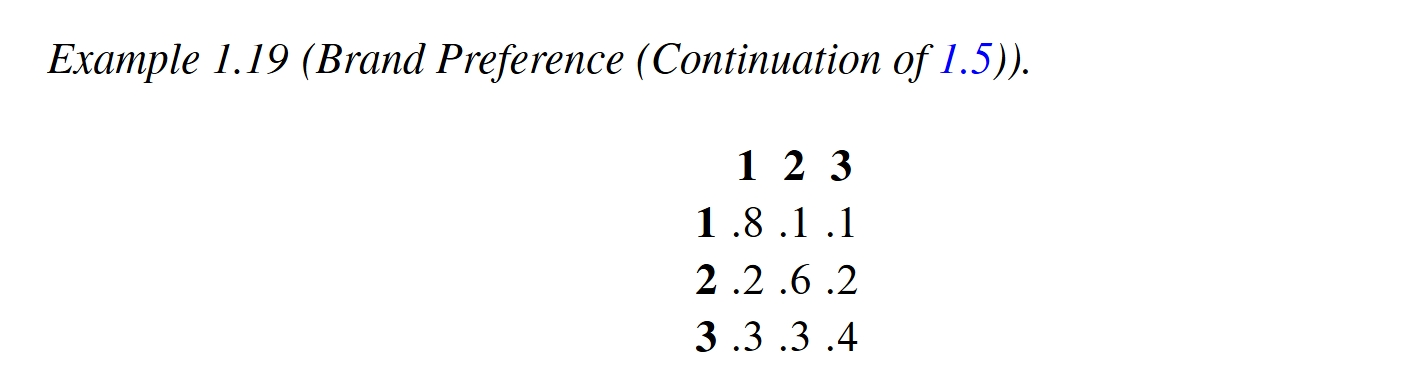
\includegraphics[width=0.9\textwidth]{figures/1_19.png}
    \end{figure}
\end{example}
\[
P-\II=\begin{bmatrix}
    -0.2 & 1 & 1\\
    0.2 & -0.4 & 0.2\\
    0.3 & 0.3 & -0.6
\end{bmatrix}
\]
\[
\begin{cases}
    \pi P=\pi\\
    \sum_{x}\pi_x=1(\pi_x\geq 0,\forall x)
\end{cases}\quad \Rightarrow \quad
\begin{cases}
    -0.2\pi_1+0.2\pi_2+0.3\pi_3=0\\
    \pi_1-0.4\pi_2+0.3\pi_3=0\\
    \pi_1+0.2\pi_2-0.6\pi_3=0\\
    \pi_1+\pi_2+\pi_3=1
\end{cases}
\]
前三个等式是线性相关的, 删去一个等式
\[
A=\begin{bmatrix}
    -0.2 & 1 & 1\\
    0.2 & -0.4 & 1\\
    0.3 & 0.3 & 1
\end{bmatrix},\quad b=[0,0,1]
\]
$\pi A=b\Rightarrow \pi=bA^{-1}$, 即 $A^{-1}$ 的最后一行

\newpage
\subsection{极限行为与平稳分布的存在唯一性}
研究 $\displaystyle \lim_{n\to \infty}p_{ij}^{(n)}$
\begin{enumerate}
    \item 由 \eqref{eq:transient_multistep}, $j$暂留 $\displaystyle\Rightarrow \sum_{n\geq 0}p_{ij}^{(n)}<\infty,\forall i\in S\Rightarrow \lim_{n\to \infty}p_{ij}^{(n)}=0,\forall i\in S$. 下面可以把注意力放在常返上
    \item $\displaystyle\lim_{n\to \infty}p_{ij}^{(n)}$不存在的反例
    \[
    S=\{1,2\}, P=\begin{pmatrix}
        0&1\\
        1&0
    \end{pmatrix}, P^2=\begin{pmatrix}
        1&0\\
        0&1
    \end{pmatrix}
    \]
    \[
    P^{2n}=\begin{pmatrix}
        1&0\\
        0&1
    \end{pmatrix}, P^{2n+1}=P=\begin{pmatrix}
        0&1\\
        1&0
    \end{pmatrix}
    \]
    $p_{ij}^{(2n)}\neq p_{ij}^{(2n+1)},\forall i,j\in S$, 所以 $p_{ij}^{(n)}$ 不收敛
\end{enumerate}

\begin{definition}[周期]\label{def:cycle}
    令 $I_x:=\{n\geq 1|P_{xx}^{(n)}>0\}$, 定义 $x$ 的周期 $d(x)=\gcd(I_x)$
    \begin{enumerate}
        \item $d(x)>1$, 称 $x$ 周期的
        \item $d(x)=1$, 称 $x$ 非周期的
        \item $I_x=\emp$, 称 $x$ 周期为 $\infty$
    \end{enumerate}
    注: $\gcd$ 为 greatest common divisor 最大公因数.
\end{definition}

\begin{definition}
    称链是周期的, 若所有状态是周期的
\end{definition}

\begin{theorem}[收敛定理]
    马氏链不可约, 非周期, 且存在平稳分布 $\pi$, 则
    \[
    \lim_{n\to\infty}p_{ij}^{(n)}=\pi_j\quad (\forall i,j\in S)
    \]
    注:找到周期不是件容易的事, 我们通常讨论非周期的链
\end{theorem}

\begin{problem}[作用7-1]
    设 $S$ 有限, $\exists i\in S$, \stt $\lim_{n\to\infty}p_{ij}^{(n)}=\pi_j(\forall j\in S)$. 证明:$\pi=(\pi_j)_{j\in S}$是$P=(p_{ij})_{i,j\in S}$的平稳分布
\end{problem}

\begin{theorem}[渐进频率]\label{thm:asymptotic_frequency}
    马氏链不可约, 常返, 则
    \begin{equation}
\lim_{n\to\infty}\frac{N_n(y)}{n}=\frac{1}{\EE_yT_y}
\end{equation}
    注:\begin{enumerate}
        \item $N_n(y)=\sum_{k=1}^n\II_{\{X_k=y\}}$($n$时刻前, 访问$y$的总次数)
        \item 考虑 $\displaystyle\frac{N_n(y)}{n}$, 表示 $n$ 时刻前访问$y$的频率/时间比例, 因此 $\displaystyle\lim_{n\to\infty}\frac{N_n(y)}{n}$ 为在状态 $y$ 上花费的时间比例的极限
        \item $\displaystyle \EE_yT_y=\begin{cases}
            <\infty & $y\text{正常返}$\\
            \infty & $y\text{暂留/零常返}$
        \end{cases}$, rf. (Def \ref{def:recurrent_types}).
    \end{enumerate}
\end{theorem}

\begin{proof}
Durrett (3ed), Thm 1.20, p47.
\end{proof}

\begin{theorem}\label{thm:stationary_exists_unique}
    马氏链不可约
    \begin{enumerate}
        \item (平稳分布唯一性, Durrett, Thm 1.21) 若平稳分布存在, 则
        \begin{equation}
\pi_y=\frac{1}{\EE_yT_y}
\label{eq:thm1.21}
\end{equation}
        则$\pi$唯一
        \item (平稳测度存在性) 若马氏链常返, 则 $\exists$平稳测度, $\mu=(\mu_x)_{x\in S}$, 且 $\mu_x>0,\forall x$. 令 $T_x=\min\{n\geq 1|X_n=x\}$.
        \begin{equation}
\mu_x(y)=\sum_{n=0}^{\infty}\PP_x(X_n=y,T_x>n)
\label{eq:stationary_measure}
\end{equation}
    \end{enumerate}
    注:$\mu=(\mu_x)_{x\in S}$ 是一个平稳测度, 若
    \begin{enumerate}
        \item (测度) $\mu_x\geq 0,\forall x\in S$
        \item $\mu P=\mu$
    \end{enumerate}
\end{theorem}

\begin{proof}
\begin{enumerate}
\item \eqref{eq:thm1.21}: Durrett (3ed), Thm 1.21, p47.
\item \eqref{eq:stationary_measure}: Durrett (3ed), Thm 1.24, p48.
\end{enumerate}
\end{proof}

相对于上面的大定理, 下面的推论对我们更有用

\begin{corollary}
    马氏链具有有限状态, 不可约, 则
    \begin{enumerate}
        \item 存在唯一平稳分布 $\pi=(\pi_x)_{x\in S}$, 且 $\displaystyle\pi_x=\frac{1}{\EE_xT_x}>0,\forall x\in S$
        \item $\displaystyle\lim_{n\to\infty}\frac{N_n(y)}{n}=\frac{1}{\EE_xT_x}=\pi_x$
    \end{enumerate}
\end{corollary}

\begin{proof}
\begin{enumerate}
    \item $S$有限不可约, 闭集$\Rightarrow$ 不可约, 常返, rf. (Thm \ref{thm:finite-close-rec}).
    \begin{enumerate}
        \item 由Thm \ref{thm:stationary_exists_unique} (2)知, 存在$\mu=(\mu_x)_{x\in S},\mu_x\geq 0, \mu P=\mu$.令 $\displaystyle\pi_x=\frac{\mu_x}{\sum_{x\in S}\mu_x}$(正则化$\mu$), $\pi_x>0$, 且 $\displaystyle\pi P=\frac{1}{\sum_{x\in S}\mu_x}\mu P=\frac{1}{\sum_{x\in S}\mu_x}\mu=\pi$
        \item 由Thm \ref{thm:stationary_exists_unique} (1)知, $\pi$唯一且$\displaystyle\pi_x=\frac{1}{\EE_xT_x}$
    \end{enumerate}
    \item 由Thm \ref{thm:asymptotic_frequency}
\end{enumerate}
\end{proof}
\newpage

\subsection{首达时及其应用}

\begin{definition}[首达时]
    首达时(first hitting time)定义为
    \begin{equation}
        V_A:=\min\{n\geq 0|X_n\in A\}
        \label{eq:FHT}
    \end{equation}
\end{definition}

注:前面提到的首次回访时间(first passage time)是要求 $n\geq 1$, rf. \eqref{eq:def_revisit_time}.

\subsubsection{击中概率(hitting time)与离出分布}

\begin{definition}[击中概率]
    击中概率定义为
    \begin{equation}
        h_x^A:=\PP_x(V_A<\infty)
        \label{eq:HT}
    \end{equation}
    特别地,$A$为闭集,称$h_x^A$为吸收概率
\end{definition}

下面介绍 $h_x^A$ 的一个性质

\begin{lemma}
    $h^A:=(h_x^A)_{x\in S}$ 满足下列方程
    \begin{equation}
\begin{cases}
        h_x^A=1 & x\in A\\
        h_x^A=\sum_y p_{xy}h_y^A & x\notin A
    \end{cases}
\end{equation}
    其中 $x\notin A$ 的情况对应卷积 $f(x)=(f*g)(x)=\sum_{y\in s}f(y)g(x-y)$.
\end{lemma}

击中概率是上述方程的一个解,之后我们将验证其唯一性.
\begin{proof}
$x\in A\Rightarrow V_A=0$, 所以 $h_x^A = \PP_x(V_A < \infty) = 1$.

$x\notin A\Rightarrow V_A\geq 1$, 考虑一步转移情况(one step reasoning) $\leftarrow$ 证明思想
\[
h_x^A=\sum_{y\in S}\PP_x(V_A<\infty, X_1=y)=\sum_{y\in S}\PP(V_A<\infty| X_1=y,X_0=x)\PP(X_1=y|X_0=x)
\]
\begin{claim}
$\PP(V_A<\infty|X_1=y,X_0=x)=h_y^A,\forall y\in S, x\notin A$
\end{claim}
利用马氏性,
\[
\begin{aligned}
    \PP(V_A<\infty| X_1=y,X_0=x) &\xlongequal{x\notin A}\PP(\bigcup_{n\geq 1}\{X_n\in A\}|X_1=y,X_0=x)\\
    &\xlongequal{\text{Markov}}\PP(\bigcup_{n\geq 1}\{X_n\in A\}|X_1=y)\\
    &\xlongequal{\text{SMP}}\PP_y(\bigcup_{n\geq 0}\{X_n\in A\})=\PP_y(V_A<\infty)=h_y^A
\end{aligned}
\]
\end{proof}

\begin{example}
    $a,b\in S,V_a:=V_{\{a\}},V_b:=V_{\{b\}}$, 考虑 $h(x)=\PP_x(V_a<V_b)$, 则 $h=(h(x))_{x\in S}$ 满足下列方程
    \[
    \begin{cases}
        h(a)=1, h(b)=0\\
        h(x)=\sum_y p_{xy}h(y) & x\neq a,b
    \end{cases}
    \]
\end{example}
\begin{proof}
(和上述引理证明过程一样) 使用一步展开方法, 
\[
h(x)=\PP_x(V_a<V_b)=\sum_{y\in S}\PP_x(V_a<V_b|X_1=y)\PP_x(X_1=y)
\]
只需证$\PP_x(V_a<V_b|X_1=y)=h(y),\forall x\neq a,b, y\in S, \to V_a\geq 1$, 就满足 $h(x)=\sum_{y\in S}p_{xy}h(y)$.
\[
\begin{aligned}
    \text{LHS} &=\PP_x(1\leq V_a<\infty, V_a<V_b|X_1=y)\\
    &\xlongequal{x\neq a,b}\PP_x\left(\bigcup_{m\geq 1}\left\{\{X_m=a\}\cap \bigcap_{1\leq k\leq m}\{X_k\neq a,b\}\right\}\bigg|X_1=y\right)\\
    &=\PP_x\left(\sum_{m\geq 1}\left\{\{X_m=a\}\cap \bigcap_{1\leq k\leq m}\{X_k\neq a,b\}\right\}\bigg|X_1=y\right)\\
    &=\sum_{m\geq 1}\PP_x\left(\{X_m=a\}\cap \bigcap_{1\leq k\leq m}\{X_k\neq a,b\}\bigg|X_1=y\right)\\
    &\xlongequal{\text{Markov}}\sum_{m\geq 1}\PP(V_a=m,V_a<V_b|X_1=y)\\
    &\xlongequal{\text{SMP}}\sum_{m\geq 1}\PP_y(V_a=m,V_a<V_b)\\
    &=\PP_y(V_a<V_b)=h(y)
\end{aligned}
\]
\end{proof}

\begin{theorem}\label{thm:fht-unique}
    $A,B\st S,A\cap B=\emp$, 令 $C=S-A\cup B$. 若 $C$ 有限, $\PP_x(V_A\land V_B<\infty)>0, \forall x\in C$, 则方程
    \begin{equation}
\begin{cases}
        h(x)=1 & x\in A\\
        h(x)=\sum_{y\in S}p_{xy}h(y) & x\in C\\
        h(x)=0 & x\in B
    \end{cases}
\end{equation}
    存在唯一非负解 $h(x)=\PP_x(V_A<V_B), \forall x\in S$ (不证明)
\end{theorem}

注:\begin{enumerate}
		\item $\land$ 是取小符号, $V_A\land V_B:=\min\{V_A,V_B \}$
    \item $\PP_x(V_a\land V_b<\infty)>0\iff x\to a \text{ 或 } x\to b$
    \item $A\cap B=\emp$ 时, $V_A\land V_B=V_{A\cup B}$
\end{enumerate}

\begin{problem}[作业8-1]
    证明:
    \begin{enumerate}
\item $\PP_x(V_a\land V_b<\infty)>0\iff x\to a \text{ 或 }x\to b$
\item $A\cap B=\emp$ 时, $V_A\land V_B=V_{A\cup B}$
\end{enumerate}
\end{problem}

\begin{figure}[H]
    \centering
    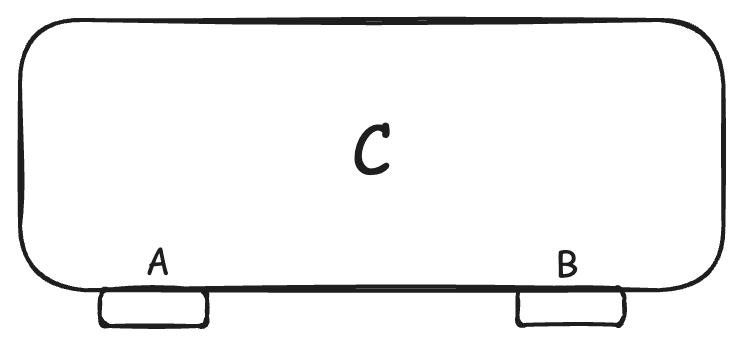
\includegraphics[width=0.35\textwidth]{figures/first-hitting.png}
    \caption{An example}
\end{figure}

$\tau_C=\min\{n\geq 0|X_n\notin C\}$ 为首次离出时刻/逃逸时刻.

$\tau=\min\{n\geq 0|X_n\in A\cup B\}, A\cap B=\emp$.

$\PP_x(X_{\tau_C}\in A)=\PP_x(V_A<V_B)$ 为逃逸概率/离出分布.

特别的, $A=\{a\}, B=\{b\}$, $a,b$ 为吸收态, $x\to a(x\neq a)$, $a\nrightarrow x, \rho_{ax}=0<1$, 由 Lem \ref{lem:commu_recurrent}, $x$ 暂留. 

$\PP_x(V_a<V_b)=\PP_x(V_a<\infty)$ 为吸收概率.

$\tau_C=V_{A\cup B}=V_A\land V_B$

$\therefore \PP_x(V_A\land V_B<\infty)=\PP_x(\tau_C<\infty)>0$.

\begin{example}\label{exa:1.43}
    $X_n$: 财富, $X_n=0$或$N$时游戏结束, 问: 赌徒破产概率.
\end{example}
\begin{proof}[解]
    \[
    \begin{cases}
        p(x,x+1)=p & 0<x<N\\
        p(x,x-1)=q=1-p & 0<x<N\\
        p(0,0)=1,p(N,N)=1 & x=0,x=N
    \end{cases}
    \]
    $0,N$ 为吸收态. 令 $h(x):=\PP_x(V_0<\infty)=\PP_x(V_0<V_N)$, $x=1,\cdots,N-1$. $S$ 有限, 不可约, 则 $\forall 0<x<N, x\to 0, x\to N$.
    \begin{figure}[H]
        \centering
        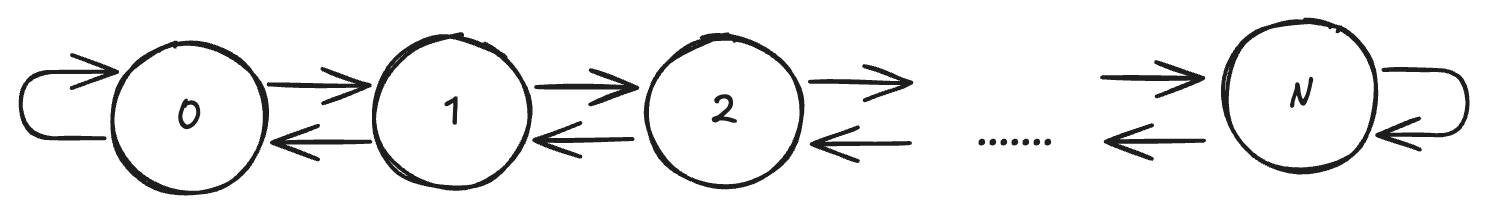
\includegraphics[width=0.55\textwidth]{figures/exa_p79.png}
    \end{figure}
    由 Thm \ref{thm:fht-unique}, $h(x)=(h(x))_{x\in S}$ 是下列方程的唯一非负解.
    \[
    \begin{cases}
        h(0)=1, h(N)=0\\
        h(x)=\sum_y p_{xy}h(y)=p(x,x+1)h(x+1)+p(x,x-1)h(x-1) & 0<x<N\\
    \end{cases}
    \]
    $h(x)=ph(x+1)+qh(x-1), 0<x<N$. $p(h(x+1)-h(x))=q(h(x)-h(x-1))$.
    \[
    h(x+1)-h(x)=\frac{q}{p}(h(x)-h(x-1))=\left(\frac{q}{p}\right)^x(h(1)-h(0)),\quad \forall 0\leq x\leq N
    \]
    \[
    \begin{aligned}
    h(x) &=h(0)+\sum_{k=0}^{x-1}(h(k+1)-h(k))\\
    &=h(0)+(h(1)-h(0))\sum_{k=0}^{x-1}\left(\frac{q}{p}\right)^x,\quad \forall 0\leq x\leq N
    \end{aligned}
    \]
    令 $\theta=q/p$.
\begin{enumerate}
    \item $\theta=1$ 时, $h(x)=h(0)+x(h(1)-h(0))$, $0=h(N)=1+N(h(1)-h(0))$, $h(1)-h(0)=-1/N$, $h(x)=1+(-1/N)x=(N-x)/N$
    \item $\theta\neq 1$ 时, 同理.
\end{enumerate}
\end{proof}
还有一种用线性代数方法求

$h[A]:=(h(x))_{x\in A}$ (列), $P[C,C]=(p_{ij})_{i,j\in C}$, $h(x)=\PP_x(V_A<V_B)$.
\[
\begin{cases}
h(x)=1 & x\in A\\
h(x)=0 & x\in B\\
h(x)=\sum_{y\in S}p_{xy}h(y) & x\in C
\end{cases}\Rightarrow 
\begin{cases}
    h[A]=\mathbf{1}\\
    h[B]=\mathbf{0}\\
    h[C]=P[C,C]h[C]+P[C,A]\mathbf{1}
\end{cases}
\]
因为 $A,B,C$ 互不相交, 
\[
\begin{aligned}
h(x)&=\sum_{y\in S}p_{xy}h(y)\\
&=\sum_{y\in A}p_{xy}h(y)+\sum_{y\in B}p_{xy}h(y)+\sum_{y\in C}p_{xy}h(y)\\
&=\sum_{y\in A}p_{xy}+\sum_{y\in C}p_{xy}h(y)\\
&=(P[x,A])_{x\in C}\mathbf{1}+(P[x,C])_{x\in C}(h(y))_{y\in C}\\
&=P[C,A]\mathbf{1}+P[C,C]h[C],\forall x\in C
\end{aligned}
\]
$\Rightarrow h[C]=(I_{|C|}-P[C,C])^{-1}P[C,A]\mathbf{1}$

\subsubsection{平均首达时与离出时刻}

\begin{definition}
    定义平均首达时.
    \[
    k_x^A:=\EE[V_A|X_0=x]=\begin{cases}
        \sum_{n\geq 0}n\PP_x(V_A=n) & \PP_x(V_A<\infty)=1\\
        \infty & \PP_x(V_A=\infty)>0
    \end{cases}
    \]
\end{definition}
\textcolor{red}{思考:} $\PP_x(V_A<\infty)=1$ 与常返的区别是? 

常返 $\PP_x(T_x<\infty)=1$ 是 $\PP_x(V_A<\infty)=1$ 的充分不必要条件.

\begin{lemma}
    $k^A=(k_x^A)_{x\in S}$ 满足
    \[
    \begin{cases}
        k_x^A=0 & x\in A\\
        k_x^A=1+\sum_{y\in S}p_{xy}k_y^A & x\notin A
    \end{cases}
    \]
\end{lemma}

\begin{proof}
当 $x\in A$ 时, $V_A=0, k_x^A=0$. 当 $x\notin A$ 时,
\[
\EE_x V_A=\sum_{y\in S}\EE_x[V_A\II_{\{X_1=y\}}]\xlongequal{\text{Cor }\eqref{cor:con_exp_indic}}\sum_{y\in S}\EE_x[V_A|X_1=y]\PP_x(X_1=y)
\]
\begin{claim}\label{claim:w8-hw2}
$\EE_x[V_A|X_1=y]=\EE[V_A+1|X_0=y], \forall y\in S, x\notin A$.
\end{claim}
\begin{proof}
见 HW Week8 作业2.
\end{proof}
将 Claim \ref{claim:w8-hw2} 代回 $\EE_x V_A$.
\[
\begin{aligned}
\sum_{y\in S}\EE_x[V_A|X_1=y]\PP_x(X_1=y)&=\sum_{y\in S}p_{xy}(1+\EE[V_A|X_0=y])\\
&=\sum_{y\in S}p_{xy}+\sum_{y\in S}p_{xy}k_y^A\\
&=1+\sum_{y\in S}p_{xy}k_y^A
\end{aligned}
\]
\end{proof}

\begin{theorem}\label{thm:p81}
    令 $C=S-A, A\st S$. 若 $C$ 有限, 且 $\forall x\in C, \PP_x(V_A<\infty)$=1. 则
    \begin{equation}
    \begin{cases}
        g(x)=0 & x\in A\\
        g(x)=1+\sum_{y\in C}p_{xy}g(y) & x\in C
    \end{cases}
    \end{equation}
    存在唯一非负解 $g(x)=\EE_xV_A$. 
\end{theorem}
$g[C]=\mathbf{1}+P[C,C]g[C]$. $g[C]=(I_{|C|}-P[C,C])^{-1}\mathbf{1}\overset{\text{书上}}{=}(\mathbf{I}-\mathbf{\gamma})^{-1}\mathbf{1}$

继续 Gambler's Ruin 例题

离出时刻 $\tau_C:=\min\{n\geq 0|X_n\neq C\}=V_{C^c}$

离出分布 $X_{\tau_C}$ 的分布
\begin{enumerate}
    \item $X_{\tau_C}\in C^c$, 故 $\{X_{\tau_C}=C^c\}=\Omega$
    \item 令 $x\in C,A\st C^c,\PP_x(X_{\tau_C}\in A)=\PP_x(V_A<V_{C^c})$
\end{enumerate}

\begin{example}[等待HT出现的时间]\label{exa:1.48}
    $X_n$: $n+1$ 时刻硬币朝上的图案, $n\geq 0$, $S_x=\{H,T\}$. 令 $Y_n=(X_n,X_{n+1}),n\geq 0$, 考虑其为马氏链且 $S=\{HH,HT,TH,TT\}$.
    \begin{align*}
        \mathbf{P}=~
        \bordermatrix{
        &\bf HH&\bf HT&\bf TH&\bf TT \cr
        \bf HH&0.5&0.5&0&0 \cr
        \bf HT&0&0&0.5&0.5 \cr
        \bf TH&0.5&0.5&0&0 \cr
        \bf TT&0&0&0.5&0.5 \cr
        }~
    \end{align*}
    令 $T_{HT}$ 为出现 $HT$ 所需的硬币投掷数. 求 $\EE T_{HT}$.
\end{example}

\begin{proof}[解]
    $A=\{HT\}, V_A:=\min\{n\geq 0|Y_n=(X_n,X_{n+1})\in A\}$, $T_{HT}=V_A+2$
    
    (Step 1) 求 $\EE_xV_A$. $S$ 有限, 不可约. 由 Thm \ref{thm:p81}, $g(x):=\EE_xV_A$ 是下列方程的唯一非负解.
    \[
    \begin{cases}
        g[A]=0\\
        g[C]=\mathbf{1}_{|C|}+P[C,C]g[C]
    \end{cases}
    \]
    \[
    g[C]=(I_{|C|}-P[C,C])^{-1}\mathbf{1}_{|C|}=\begin{bmatrix}
        2\\2\\4
    \end{bmatrix}\begin{matrix}
        \bf HH \\ \bf TH\\ \bf TT
    \end{matrix}
    \]
    (Step 2)
    \[
    \begin{aligned}
        \EE T_{HT}&=2+\EE V_A\\
        &=2+\sum_{x\in S}\EE V_A\II_{\{Y_0=x\}}\\
        &\xlongequal{\text{Cor }\eqref{cor:con_exp_indic}}2+\sum_{x\in S}\EE[V_A|Y_0=x]\PP(Y_0=x)\\
        &=2+\sum_{x\in S}g(x)\PP(X_0=H,X_1=T)\\
        &=2+\frac{1}{4}(0+2+2+4)=4
    \end{aligned}
    \]
\end{proof}
\newpage
\subsection{具有无限状态的马氏链}

\begin{figure}[H]
    \centering
    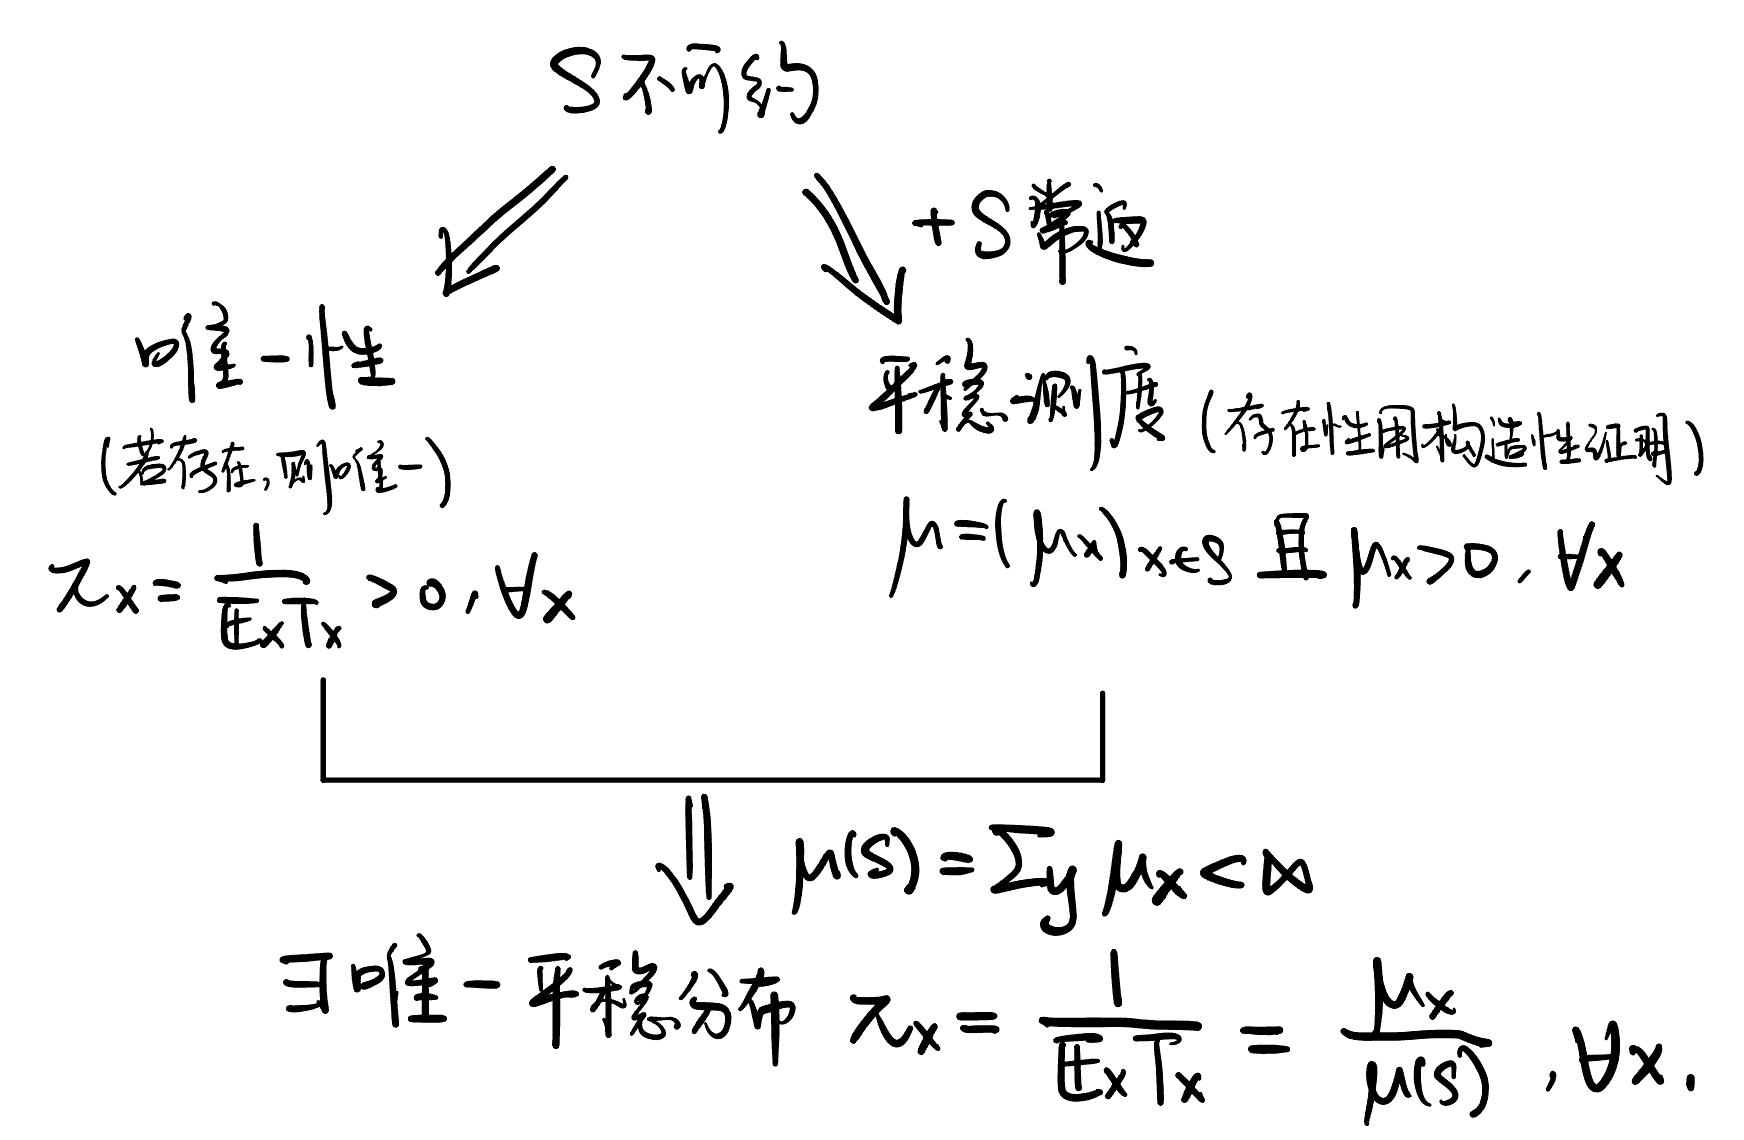
\includegraphics[width=0.65\textwidth]{figures/irreduce_summary.png}
    \caption{Summary}
\end{figure}

``构造性证明'' 见 \eqref{eq:stationary_measure}.

\begin{claim}
$S$ 不可约, 若存在平稳分布, 则 $\pi_x>0,\forall x\in S$.
\end{claim}

\begin{proof}
    设 $\exists x, \stt \pi_x=0$. $\pi=\pi P^n, \forall n\geq 0$. $\pi_x=\sum_y\pi_y p_{yx}^{(n)}, \forall n\geq 0$. $\Rightarrow \pi_y p_{yx}^{(n)}=0,\forall y\in S,n\geq 0$. 又因 $S$ 不可约, $\forall y\in S, y\to x$. 所以 $\exists n_y\geq 0, \stt p_{yx}^{(n_y)}>0$. $\Rightarrow \forall y\in S, \pi_y=0$. 这与 $\sum_y\pi_y=1$ 矛盾
\end{proof}

\begin{lemma}\label{lem:p84}
    $S$不可约, \framebox{若存在平稳测度 $\mu=(\mu_x)_{x\in S},\mu_x>0,\forall x$} (即``若 $S$ 常返成立''), \framebox{$\mu(S)=\sum_{x\in S}\mu_x<\infty$}, 则存在唯一平稳分布
    \begin{equation}
    \pi_x=\frac{1}{\EE_xT_x}=\frac{\mu_x}{\mu(S)}>0,\forall x
    \end{equation}
    注: $\pi_x=1/(\EE_xT_x)>0,\forall x$ 为必要条件

    $\Rightarrow \EE_xT_x<\infty, \forall x\Rightarrow \forall x$, $x$ 正常返 $\Rightarrow$ $S$正常返. (这是必要条件, 那反过来是否充分? 能否推出框内条件?)
\end{lemma}

$i \leftrightarrow j$, 则由 Cor \ref{cor:trans_recurrent}, $i$正常返 $\iff$ $j$正常返, $i$零常返 $\iff$ $j$零常返, $i$非周期 $\iff$ $j$非周期. $p_{jj}>0\Rightarrow d(j)=1$. 

\begin{theorem}
    $S$ 不可约, 则下列结论等价
    \begin{enumerate}
        \item 某个状态正常返
        \item 存在平稳分布 $\pi$
        \item 所有状态正常返
    \end{enumerate}
\end{theorem}

\begin{proof}
    $(3)\Rightarrow (1)$ 显然, $(2)\Rightarrow (3)$ 在上面注记中已证. 要证 $(1)\Rightarrow (2)$.

    $S$不可约, 存在$x$正常返 $\Rightarrow$ $S$不可约, 常返. 由 Thm \ref{thm:stationary_exists_unique} 及 \eqref{eq:stationary_measure}, 存在平稳测度 $\mu_y=\sum_{n\geq 0}\PP_x(T_x>n,X_n=y),\forall y\in S$. 由 Lem \ref{lem:p84} 框内条件知, 平稳测度要求 $\mu(S)<\infty$.
    \[
    \begin{aligned}
        \mu(S) = \sum_{y\in S}\mu_y
        &=\sum_{n\geq 0}\sum_{y\in S}\PP_x(T_x>n,X_n=y)\\
        &=\sum_{n\geq 0}\PP_x(T_x>n)=\EE_x T_x<\infty
    \end{aligned}
    \]
    注: $T_x=\sum_{n\geq 0}\II_{\{T_x>n\}}=\sum_{n\geq 1}\II_{\{T_x\geq n\}}$.

    存在平稳分布 $\pi_x=\mu_x/\mu(S)>0,\forall x$.
\end{proof}

\begin{corollary}
    对不可约链, 下列情况之一必发生
    \begin{enumerate}
        \item $S$非常返, 则不存在平稳分布
        \item $S$常返, 则对 $\forall x\in S$, 存在平稳测度 $\mu^{(x)}=(\mu_y^{(x)})_{y\in S}$. (由 Thm \ref{thm:stationary_exists_unique} 定义).
        \begin{enumerate}
            \item $\forall x,\mu^{(x)}(S)=\EE_xT_x<\infty$, 则$S$正常返, 则存在唯一平稳分布
            \item $\forall x,\mu^{(x)}(S)=\EE_xT_x=\infty$, 则$S$零常返, 则不存在平稳分布
        \end{enumerate}
    \end{enumerate}
\end{corollary}

\subsubsection{广义生灭链}

\begin{example}[带反射壁的随机游动(Durrett 1.54)]
    质点在 $S=\{0,1,2,\cdots\}$ 移动, 规定
    \begin{figure}[H]
        \centering
        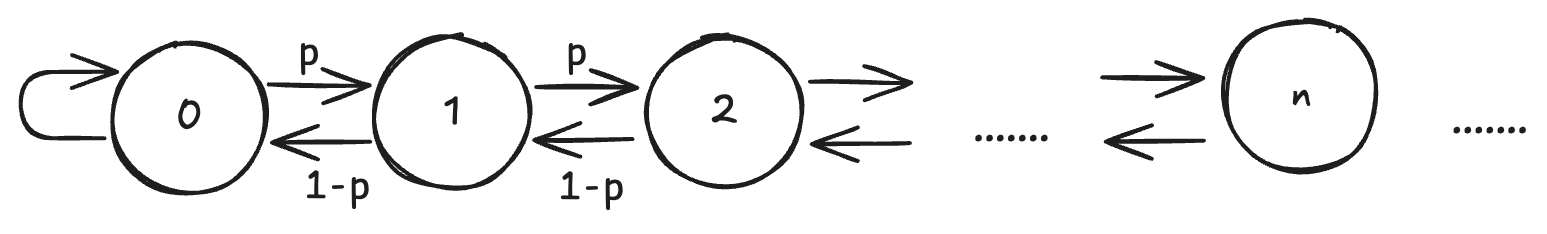
\includegraphics[width=0.65\textwidth]{figures/g_birth_death.png}
    \end{figure}
    $p\in (0,1)$, $X_n$: 表示 $n$ 时刻质点所在位置. 则
    \begin{enumerate}
        \item $p\in (0,1/2)$ 时, 存在唯一平稳分布, $S$ 正常返
        \item $p>1/2$ 时, $S$ 非常返, 不存在平稳分布
        \item $p=1/2$ 时, $S$ 零常返, 不存在平稳分布
    \end{enumerate}
\end{example}

\begin{proof}
\begin{enumerate}
    \item (Step 1) $S$不可约, 则平稳分布若存在则唯一
    
    (Step 2) (存在性) 回顾 Exa \ref{exa:birth_death}, 与当前例子的区别是状态空间 $S$ 是否有限. 设 $\pi$ 满足DBC, $\pi_xp_{xy}=\pi_yp_{yx},\forall x,y$. $\pi_ip_{i,i+1}=\pi_{i+1}p_{i+1,i},\forall i\geq 0$. $\pi_i p=\pi_{i+1}(1-p),\forall i\geq 0$.
    \[
    \pi_{i+1}=\frac{p}{1-p}\pi_i=\left(\frac{p}{1-p}\right)^{i+1}\pi_0,\forall i\geq 0
    \]
    \[
    \pi_i=\left(\frac{p}{1-p}\right)^{i}\pi_0,\forall i\geq 0\tag{*}
    \]
    又由 $\sum_i \pi_i=1$, 有
    \[
    1=\pi_0\sum_{i\geq 0}\left(\frac{p}{1-p}\right)^i=\pi_0\frac{1}{1-\frac{p}{1-p}}\Rightarrow \pi_0=\frac{1-2p}{1-p}\in (0,1)
    \]
    代回 $(*)$, 得 $\pi_i>0,\forall i$. 其中无穷级数 $\sum_{i\geq 0}\left(\frac{p}{1-p}\right)^i$ 当 $|p/(1-p)|<1$ 时收敛, 即 $p<1/2$ 时. ($\sum_{i=0}^{\infty}r^i=1/(1-r), \forall |r|<1$)
    \item 只需证状态 $0$ 暂留, 又因为 $0\to 1$, Lem \ref{lem:commu_recurrent}, 故只需证 $1>\rho_{1,0}=\PP_1(T_0<\infty)=\PP_1(V_0<\infty)$. 考察 $\PP_x(V_0<\infty)$. 注意到
    \[
    \{V_0<\infty,X_0=x\neq 0\}=\bigcup_{M\geq 0}\{V_0=M,X_0=x\neq 0\}=\bigcup_{M\geq 0}\bigcup_{N\geq x+M}\{V_0<V_N,X_0=x\neq 0\}
    \]
    $X_0=x\neq 0, \forall N\geq x+M+10000000$, $M=V_0<V_N<V_{N+1}$.

    令 $h(x):=\PP_x(V_0<V_N)$, 则
    \[
    \begin{cases}
        h(0)=1,h(N)=0\\
        h(x)=ph(x+1)+(1-p)h(x-1) & \forall x\neq 0,N
    \end{cases}
    \]
    由 Exa \ref{exa:1.43}, $\theta=(1-p)/p<1$ 时, $h(x)=(\theta^x-\theta^N)/(1-\theta^N),\forall x\in S$.
    \item 考虑一步转移情况.
    \[
    \begin{aligned}
        \EE_0T_0 &= \EE_0[T_0\II_{\{X_1=0\}}]+\EE_0[T_0\II_{\{X_1=1\}}]\\
        &=\EE_0[T_0|X_1=0]p_{0,0}+\EE_0[T_0|X_1=1]p_{0,1}\\
        &\xlongequal{\text{Markov}}\EE[V_0+1|X_0=0]\frac{1}{2}+\EE[V_0+1|X_0=1]\frac{1}{2}\\
        &=\frac{1}{2}(\EE_0(1)+\EE_1(1))+\frac{1}{2}\EE_1V_0\\
        &=1+\frac{1}{2}\EE_1V_0
    \end{aligned}
    \tag{*}
    \]
    考察 $g(x)=\EE_xV_0$.

    (Step 1) 考察 $\EE_x(V_0\land V_N)$, 同 Exa \ref{exa:1.48} 类似计算得到 $\EE_x(V_0\land V_N)=x(N-x)$.

    (Step 2) $\EE_1V_0\geq \EE_1(V_0\land V_N)=N-1\to +\infty, (N\to +\infty)$. 代回 $(*)$ 得 $\EE_0T_0=+\infty$
\end{enumerate}
\end{proof}
\newpage

\pagebreak

\section{泊松过程}
\subsection{指数分布, 泊松分布}

\subsubsection{指数分布}

\begin{definition}[指数分布]
    称随机变量 $T$ 服从 ``参数/速率$\lambda(\lambda>0)$的指数分布'', 记作 $T\sim \EXP(\lambda)$, 若分布
    \begin{equation}
        F_T(t)=\begin{cases}
            1-e^{-\lambda t} & t\geq 0\\
            0 & t<0
        \end{cases}
    \end{equation}
    \begin{equation}
        f_T(t)=\begin{cases}
            \lambda e^{-\lambda t} & t\geq 0\\
            0 & t<0
        \end{cases}
    \end{equation}
\end{definition}

\begin{property}[矩]
$T\sim \EXP(\lambda)$, 则
\begin{enumerate}
    \item $\EE T=1/\lambda$
    \item $\EE T^2=2/\lambda^2$
    \item $\Var(T)=\EE T^2-(\EE T)^2=1/\lambda^2$
\end{enumerate}
\end{property}

\begin{property}[Scaling]
$T\sim \EXP(\lambda), S\sim \EXP(1)$, 则 $S/\lambda\overset{(d)}{=}T, S\overset{(d)}{=}\lambda T$.
\end{property}

\begin{property}[无记忆性]
$T\sim \EXP(\lambda)$, 则 $\PP(T>t+s|T>t)=\PP(T>s)$

注: 等价于 $\bar{F}(t+s)=\bar{F}(t)\bar{F}(s)$, 其中 $\bar{F}(t):=1-F(t)$.
\end{property}

\begin{property}[指数分布的排序]
$T_i\sim \EXP(\lambda_i)$, 独立. 令 $V=\min\{T_1,T_2,\cdots,T_n\}$, $I:=\min\{i|T_i=V\}$ (随机下标)
\begin{enumerate}
    \item $V\sim \EXP\left(\sum_{k=1}^n\lambda_k\right)$, 即
    \begin{equation}
		\PP(V>t)=\exp\left(-\sum_{k=1}^n\lambda_k \cdot t\right)
		\end{equation}
    \item $\PP(T_i=V)=\lambda_i/(\sum_{k=1}^n\lambda_k)$
    \item $I\ind V$
\end{enumerate}
\end{property}

\begin{proof}
(1) ``最短完成时间'' 的概率分布.
\[
\displaystyle\PP(V>t)=\PP(T_k>t,1\leq k\leq n)=\prod_{k=1}^n\PP(T_k>t)=\prod_{k=1}^n e^{-\lambda_k t}=\exp \left(-\sum_{k=1}^n\lambda_k\cdot t\right), t\geq 0
\]
(2) ``XX比YY先完成''的概率.

设 $S\sim\EXP(\lambda), U\sim\EXP(\mu), S\ind U$
\[
\begin{aligned}
    \PP(S=\min\{S,U\}) &=\PP(S\leq U)\\
    &\xlongequal{S\ind U}\int_0^{\infty}\PP(S\leq t)f_U(t)dt\\
    &=\int_0^{\infty}(1-e^{-\lambda t})f_U(t)dt\\
    &=1-\int_0^{\infty}e^{-\lambda t}\mu e^{-\mu t}dt\\
    &=1-\frac{\mu}{\lambda+\mu}\int_0^{\infty}(\lambda+\mu)e^{-(\lambda+\mu)t}dt=\frac{\lambda}{\lambda+\mu}
\end{aligned}
\tag{*}
\]
令 $S=T_i, U=\min\{T_1,\cdots,T_{i-1},T_{i+1},\cdots,T_n\}$, 由 (1) 结论, 则 $\lambda=\lambda_i,\mu=(\sum_{k=1}^n\lambda_k)-\lambda_i$. 代回 (*), 得 $\PP(T_i=V)=\lambda_i/(\sum_{k=1}^n\lambda_k)$.

(3) 令 $\tilde{V}_i:=\min\{T_1,\cdots,T_{i-1},T_{i+1},\cdots,T_n\}$.

$\{I=i\}=\{T_i<\tilde{V}_i\}+\cup_{j=i+1}^n\{T_i\leq \tilde{V}_i,T_i=T_j\}$. 其中 $\{T_i<\tilde{V}_i\}$ 为唯一最小, $T_i\leq \tilde{V}_i$ 中至少一个与之相等.
\[
\begin{aligned}
    \PP\left(\bigcup_{j=i+1}^n\{T_i\leq \tilde{V}_i, T_i=T_j\}\right) & \leq \sum_{j=i+1}^n\PP(T_i=T_j)\\
    &\xlongequal{T_i\ind T_j}\sum_{j=i+1}^n \int_0^{\infty}\PP(T_i=t)f_{T_j}(t)dt=0
\end{aligned}
\]
其中 $\PP(T_i=t)=0$. 由此得 $\PP(I=i)\overset{(d)}{=}\PP(T_i<\tilde{V}_i)$.
\[
\begin{aligned}
    \PP(I=i,V>t)&=\PP(T_i<\tilde{V}_i,V>t)\\
    &=\PP(\tilde{V}_i>T_i>t)\\
    &\xlongequal{T_i\ind \tilde{V}_i}\int_0^{\infty}\PP(\tilde{V}_i>s>t)f_{T_i}(s)ds\\
    &=\int_0^{\infty}\II_{s>t}\PP(\tilde{V}_i>s)f_{T_i}(s)ds\\
    &=\int_t^{\infty}\exp\left(-\sum_{k\neq i}\lambda_k\cdot s\right)\cdot\lambda_i e^{-\lambda_i s}ds\\
    &\overset{(1)}{=}\frac{\lambda_i}{\sum_{k=1}^n \lambda_k}\cdot\int_t^{\infty}\left(\sum_{k=1}^n\lambda_k\right)\exp\left(-\sum_{k=1}^n\lambda_k\cdot s\right)ds\\
    &\xlongequal{(1,2)}\PP(V>t)\PP(I=i)
\end{aligned}
\]
由 (2), $\PP(T_i=V)=\PP(T_i\leq \tilde{V}_i)=\lambda_i/(\sum_{k=1}^n \lambda_k)$. 所以 $\PP(I=i)=\PP(T_i<\tilde{V}_i)=\lambda_i/(\sum_{k=1}^n \lambda_k)$, 在测度意义上相等.
\end{proof}

\begin{theorem}[指数分布随机变量之和]
    设 $\tau_1,\tau_2,\cdots$ 独立同分布, $\tau_1\sim\EXP(\lambda)$, 则对 $n\geq 1$, 有
    \begin{equation}
        T_n=\sum_{k=1}^n\tau_k\sim \Gamma (n,\lambda)
    \end{equation}
    即
    \begin{equation}
        f_{T_n}(t)=\begin{cases}
            \lambda e^{-\lambda t}\frac{(\lambda t)^{n-1}}{(n-1)!} & t\geq 0\\
            0 & t<0
        \end{cases}
    \end{equation}
    其中 约定 $0^0=1, 0!=1$.
\end{theorem}

\begin{proof}
\begin{enumerate}
    \item $n=1$ 显然.
    \item 假设 $n=k$ 成立. 下证 $n=k+1$ 也成立.
    \[
    T_{k+1}=T_k+\tau_{k+1}, T_k\ind T_{k+1}
    \]
    \[
    \begin{aligned}
        f_{T_{k+1}}(t)&=(f_{T_k}*f_{\tau_{k+1}})(t)\\
        &=\int_0^t f_{T_k}(s)f_{\tau_{k+1}}(t-s)ds\\
        &=\int_0^t \lambda e^{-\lambda s}\frac{(\lambda s)^{k-1}}{(k-1)!}\lambda e^{-\lambda (t-s)}ds\\
        &=\frac{\lambda^{k+1}}{(k-1)!}e^{-\lambda t}\int_0^t s^{k-1}ds\\
        &=\frac{\lambda^{k+1}e^{-\lambda t}}{(k-1)!}\left[\frac{s^k}{k}\bigg|^t_0\right]=\lambda e^{-\lambda t}\frac{(\lambda t)^k}{k!}
    \end{aligned}
    \]
\end{enumerate}
\end{proof}

注: 概率密度函数之和的分布等于这两个密度函数的卷积. 从分布函数出发推导
\[
\begin{aligned}
F_Z(z) = \mathbb{P}(X + Y \leq z)&\xlongequal{X\ind Y} \iint_{x + y \leq z} f_X(x) f_Y(y) \, dx\,dy \\
&= \int_{-\infty}^\infty f_X(x) \left( \int_{-\infty}^{z - x} f_Y(y) \, dy \right) dx \\
&= \int_{-\infty}^\infty f_X(x) F_Y(z - x) \, dx
\end{aligned}
\]

对分布函数求导得到密度函数:
\[
\begin{aligned}
f_Z(z) = \frac{d}{dz} F_Z(z) &= \frac{d}{dz} \int_{-\infty}^\infty f_X(x) F_Y(z - x) \, dx \\
&= \int_{-\infty}^\infty f_X(x) \frac{d}{dz} F_Y(z - x) \, dx \\
&= \int_{-\infty}^\infty f_X(x) f_Y(z - x) \, dx \\
&= (f_X * f_Y)(z)
\end{aligned}
\]

\subsubsection{泊松分布}

\begin{definition}
    称 $X$ 服从 ``均值/参数为 $\lambda(\lambda>0)$ 的泊松分布'' (记作 $X\sim \Poi(\lambda)$), 若 
    \begin{equation}
\PP(X=n)=e^{-\lambda}\frac{\lambda^n}{n!}
\end{equation}
\end{definition}

\begin{property}[矩]
$X\sim \Poi(\lambda)$, 对 $\forall k\geq 1$, 
\begin{equation}
\EE X(X-1)\cdots (X-k+1)=\lambda^k
\end{equation}
特别地, 
\begin{enumerate}
    \item $k=1$ 时, $\EE X=\lambda$
    \item $\Var(X)=\EE X^2-(\EE X)^2=\EE X(X-1)+\EE X-(\EE X)^2\overset{k=2}{=}\lambda^2+(\lambda-\lambda^2)=\lambda$
\end{enumerate}
\end{property}

\begin{proof}
    \[
    \begin{aligned}
        \LHS &=\sum_{n=0}^{\infty}n(n-1)\cdots (n-k+1)e^{-\lambda}\frac{\lambda^n}{n!}\\
        &=\sum_{n=k}^{\infty}\frac{n!}{(n-k)!}e^{-\lambda}\frac{\lambda^n}{n!}\\
        &=\lambda^k e^{-\lambda}\sum_{n=k}^{\infty}\frac{\lambda^{n-k}}{(n-k)!}\\
        &\xlongequal{m=n-k} \lambda^ke^{-\lambda}\sum_{m=0}^{\infty}\frac{\lambda^m}{m!}\\
        &=\lambda^k e^{-\lambda}e^{\lambda}=\lambda^k
    \end{aligned}
    \]
\end{proof}

\begin{theorem}[Durrett Thm 2.4, 泊松随机变量之和]
    $X_k\sim \Poi(\lambda_k),k\geq 1$ 独立, 则
    \begin{equation}
\sum_{k=1}^N X_k\sim \Poi\left(\sum_{k=1}^N \lambda_k\right)
\end{equation}
\end{theorem}

\begin{proof}
    $N=2$. 
    \[
    \PP(X_1+X_2=n)\xlongequal{X_1\ind X_2}\sum_{m=0}^{\infty}\PP(X_1+m=n)\PP(X_2=m)
    \]
    公式: $\EE |g(X,Y)|<\infty, X\ind Y$, 则 $\EE g(X,Y)=\EE(\EE g(x,Y)|_{x=X})$.
    \[
    \begin{aligned}
        \PP(X_1+X_2=n) &=\EE \II_{\{X_1+X_2=n\}}\\
        &\xlongequal{X_1\ind X_2}\EE_{X_2}(\EE_{X_1} \II_{\{X_1+m=n\}}|_{m=X_2})\\
        &=\EE_{X_2}(\PP(X_1+m=n)|_{m=X_2})\\
        &=\sum_{m=0}^{\infty}\PP(X_1+m=n)\PP(X_2=m)
    \end{aligned}
    \]
    $\EE_{X_1},\EE_{X_2}$ 表示关于 $X_1,X_2$ 求期望. 利用独立改写成卷积.
    \[
    \begin{aligned}
        \PP(X_1+X_2=n) &\xlongequal{X_1\ind X_2} \sum_{m=0}^n \PP(X_1=n-m)\PP(X_2=m)\\
        &=\sum_{m=0}^{\infty}e^{-\lambda_1}\frac{\lambda_1^{n-m}}{(n-m)!}e^{-\lambda_2}\frac{\lambda_2^m}{m!}\\
        &=e^{-(\lambda_1+\lambda_2)}\frac{(\lambda_1+\lambda_2)^n}{n!}\cdot \sum_{m=0}^n\frac{n!}{m!(n-m)!}\left(\frac{\lambda_2}{\lambda_1+\lambda_2}\right)^m\left(\frac{\lambda_1}{\lambda_1+\lambda_2}\right)^{n-m}\\
        &=e^{-(\lambda_1+\lambda_2)}\frac{(\lambda_1+\lambda_2)^n}{n!}
    \end{aligned}
    \]
其中, 由二项式定理 $(a + b)^n = \sum_{k=0}^{n} \binom{n}{k} a^k b^{n-k}$ 知,
    \[
    \sum_{m=0}^n\frac{n!}{m!(n-m)!}\left(\frac{\lambda_2}{\lambda_1+\lambda_2}\right)^m\left(\frac{\lambda_1}{\lambda_1+\lambda_2}\right)^{n-m}=\left(\frac{\lambda_1}{\lambda_1+\lambda_2}+\frac{\lambda_1}{\lambda_1+\lambda_2}\right)^n=1
    \]
\end{proof}

\begin{theorem}[Durrett(3ed), Thm 2.5, 二项分布的泊松逼近]
    $X_n\sim \Bi(n,\frac{\lambda}{n})\xrightarrow{n\to\infty}\Poi(\lambda), \lambda>0$. 其中 $\xrightarrow{n\to\infty}$ 表示依分布收敛.
\end{theorem}

\begin{proof}
\[
\begin{aligned}
    \PP(X_n=k) &=\frac{n!}{k!(n-k)!}\left(\frac{\lambda}{n}\right)^k \left(1-\frac{\lambda}{n}\right)^{n-k}\\
    &=\frac{\lambda^k}{k!}\cdot \left[\frac{n!}{(n-k)!\cdot n^k}\cdot \left(1-\frac{\lambda}{n}\right)^n\cdot \left(1-\frac{\lambda}{n}\right)^{-k} \right]\\
    &=:\frac{\lambda^k}{k!}\cdot [\mc{J}_{n,1}\cdot \mc{J}_{n,2}\cdot \mc{J}_{n,3}]
\end{aligned}
\]
\[
\lim_{n\to\infty}\mc{J}_{n,1}=\lim_{n\to\infty}\frac{n(n-1)\cdots (n-k+1)}{n\cdot n\cdots n}=1
\]
\[
\lim_{n\to\infty}\mc{J}_{n,2}=\lim_{n\to\infty}\left[(1+\frac{-\lambda}{n})^{n/(-\lambda)}\right]^{-\lambda}=e^{-\lambda}
\]
$\lim_{n\to\infty}\mc{J}_{n,3}=1^{-k}=1$. 代回得
\[
\lim_{n\to\infty}\PP(X_n=k)=e^{-\lambda}\cdot \frac{\lambda^k}{k!}
\]
\end{proof}
\newpage
\subsection{泊松过程的定义}

\begin{definition}[计数过程]
    若随机变量 $N(t)$ 表示时间段 $[0,t]$ 内某事件发生的次数, 则称 $\{N(t),t\geq 0\}$ 是一个计数过程, 若
    \begin{enumerate}
        \item $N(t)\geq 0$ 取整数值
        \item 若 $s<t$, 则 $N(s)\leq N(t)$, 且 $N(t)-N(s)$ 表示时间段 $(s,t]$ 内事件的发生次数
    \end{enumerate}
\end{definition}

\begin{definition}[泊松过程I]\label{def:counting-process-I}
    称一个计数过程 $\{N(t),t\geq 0\}$ 是一个带有参数/速率 $\lambda(\lambda>0)$ 的泊松过程, 若
    \begin{enumerate}
        \item $N(0)=0$, 即 $\PP(N(0)=0)=1$
        \item (独立增量) $\forall 0\leq t_1<t_2<\cdots<t_n$, 有
        \[
        N(t_2)-N(t_1),\cdots,N(t_n)-N(t_{n-1})
        \]
        相互独立
        \item $\forall t>0,s\geq 0, N(t+s)-N(s)\sim \Poi(\lambda t)$
    \end{enumerate}
\end{definition}

\begin{property}
由 Def \ref{def:counting-process-I} (3) 易知, $(N(t))_{t\geq 0}$ 具有平稳增量.
\[
N(t+s)-N(s)\xlongequal{(d)} N(t)-N(0)\xlongequal{(d)}N(t)\sim \Poi(\lambda t)
\]
注: $\EE N(t)=\lambda t\Rightarrow \lambda=\EE N(t)/t$ 过程的速率
\end{property}

\begin{property}[Durrett, Lem 2.5]
对固定 $s\geq 0, \{N(t+s)-N(s),t\geq 0\}$ 仍是一个带有速率 $\lambda$ 的Poisson过程, 且 $N(t+s)-N(s)\ind N(r), \forall 0\leq r\leq s,t\geq 0$
\end{property}

\begin{definition}[泊松过程II: 到达时间间隔]\label{def:poi-2}
    令 $\tau_1,\tau_2,\cdots$ 为一列独立同分布的随机变量, $\tau_1\sim \EXP(\lambda)$,
    \[
    T_n=\begin{cases}
        \sum_{k=1}^n\tau_k & n\geq 1\\
        0 & n=0
    \end{cases}
    \]
    $N(t)=\max\{n|T_n\leq t\}$, 则称 $\{N(t),t\geq 0\}$ 为带有速率 $\lambda$ 的Poisson过程
    
    注: ``无穷小定义'', 见 Sheldon Ross 随机过程\cite{ross1995stochastic}.
\end{definition}
注:
\begin{enumerate}
    \item $T_n(n\geq 1)$: 第 $n$ 个顾客的到店时刻
    \item $\tau_n(n\geq 1)$: 第 $n$ 个和第 $n-1$ 个顾客的到店时间间隔
    \item $N(t)$: $t$ 时刻之前到达的顾客总数
\end{enumerate}
\begin{figure}[H]
    \centering
    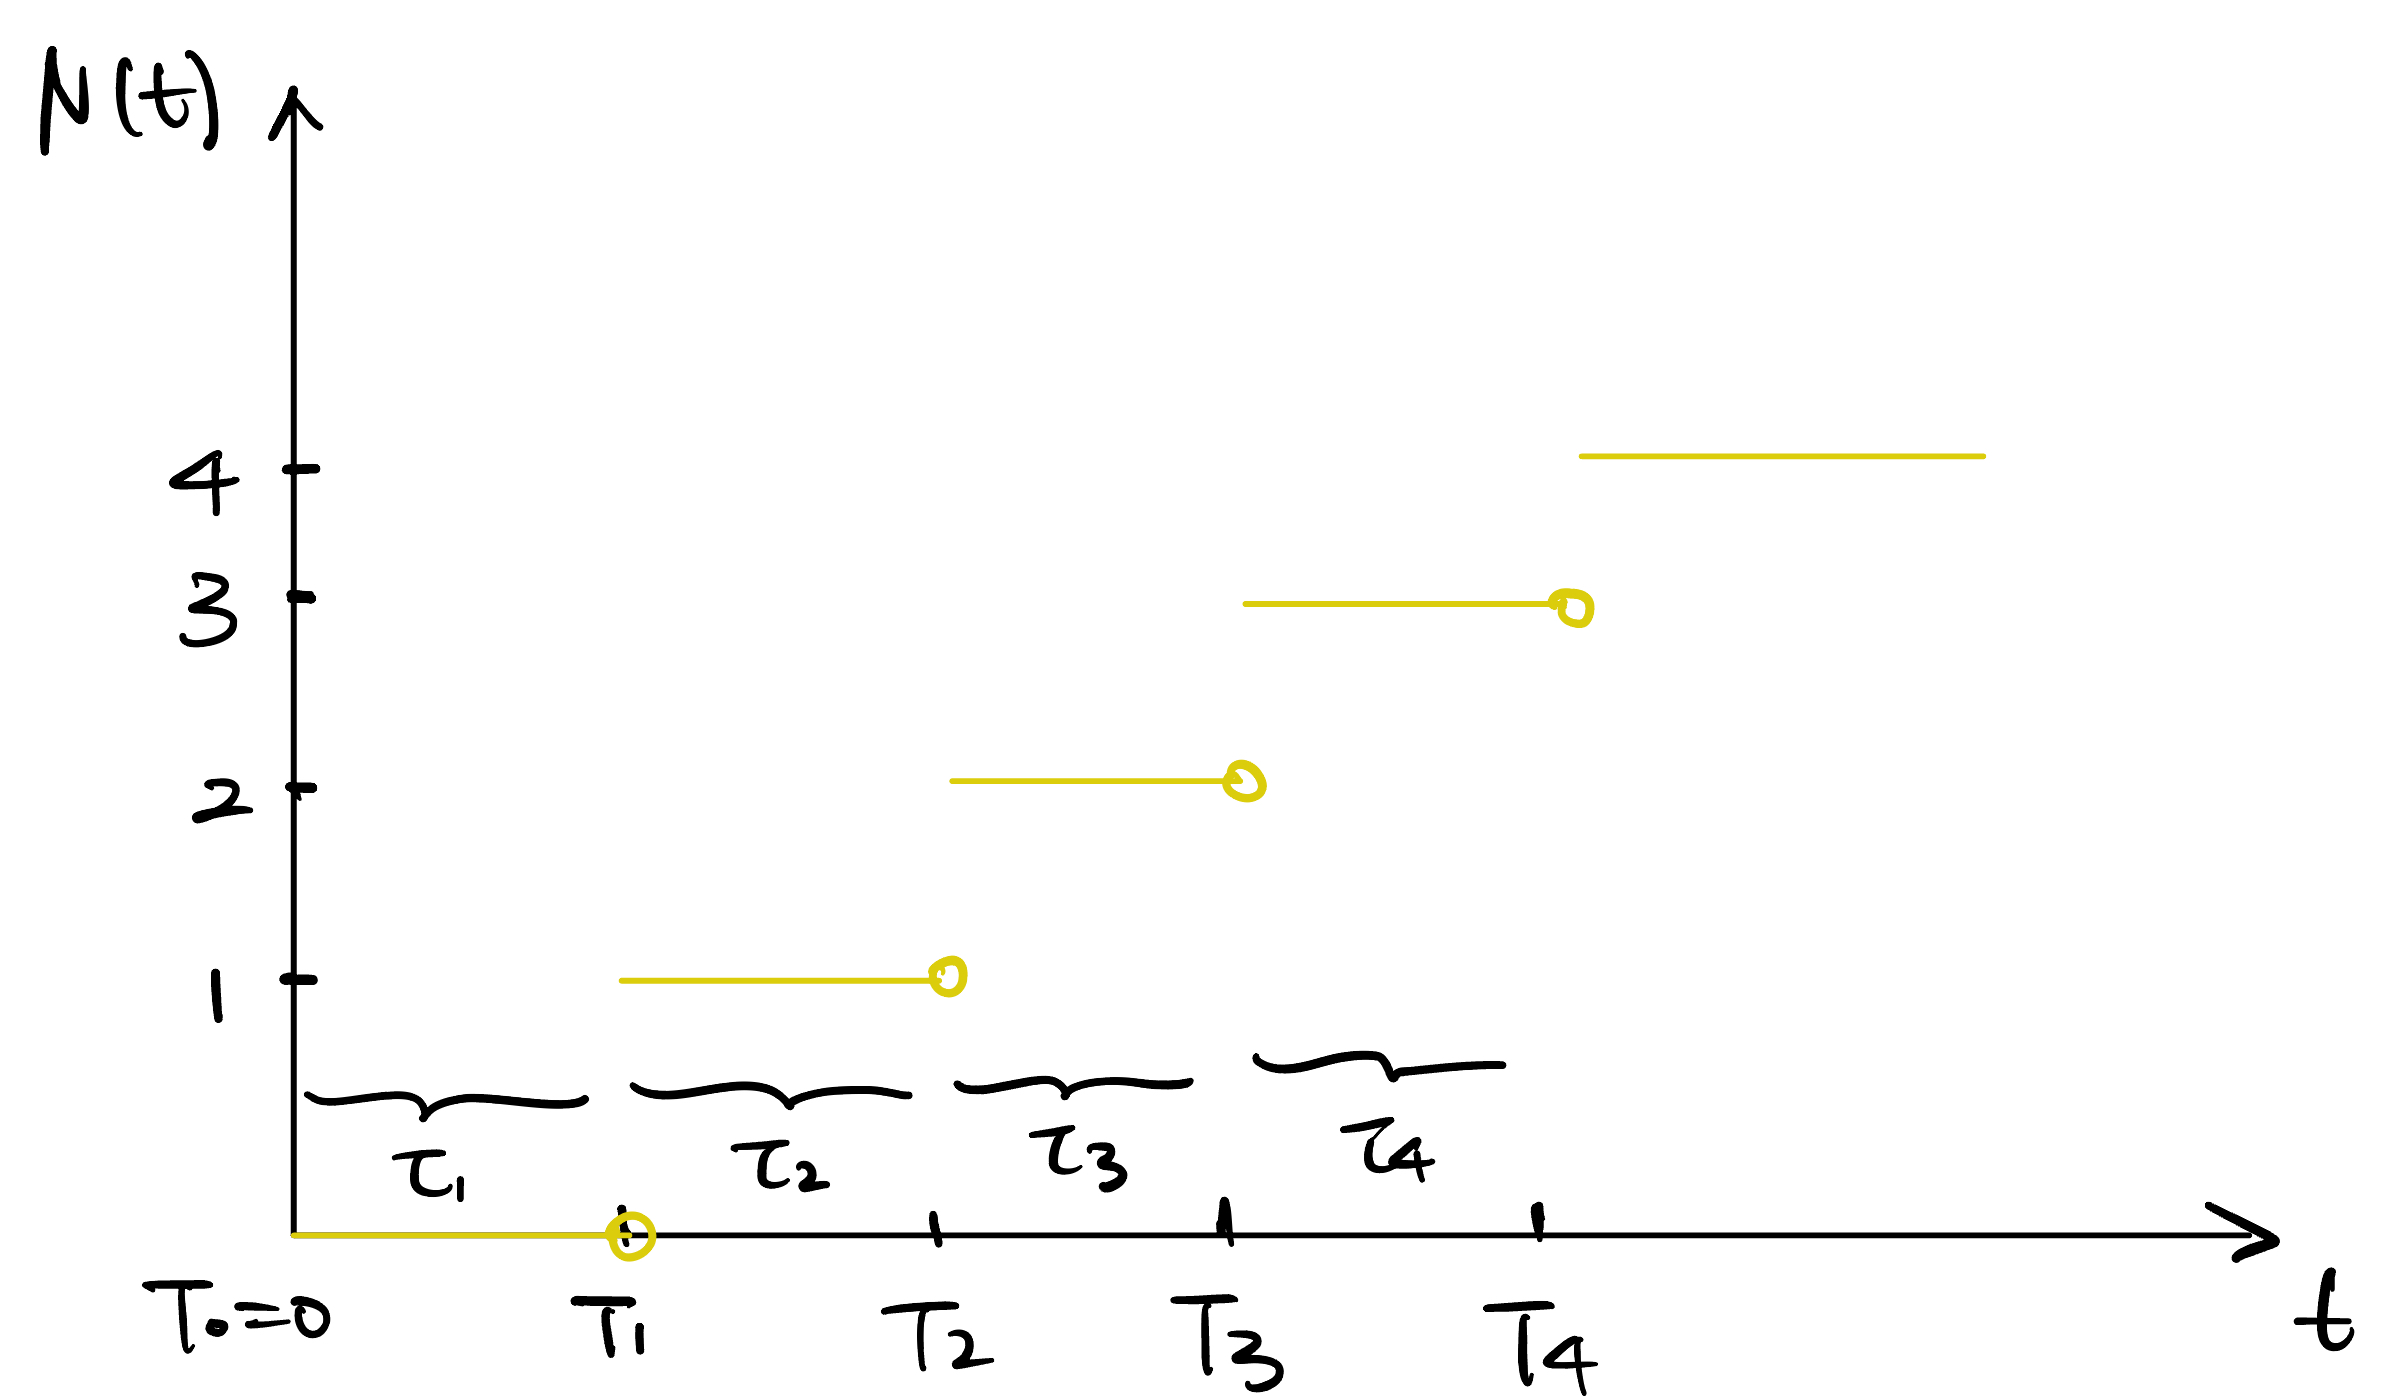
\includegraphics[width=0.65\textwidth]{figures/arrival.png}
    \caption{Arrival}
\end{figure}
注意 $T_1,T_2,\cdots$ 是随机的
\begin{enumerate}
    \item $n\geq 1, \tau_n=T_n-T_{n-1}\sim \EXP(\lambda), T_n\sim\Gamma(n,\lambda)$
    \item $\{N(t)=n\}=\{T_n\leq t< T_{n+1}\}$
    \item $\{N(t)\geq n\}=\{t\geq T_n\}$
    \item $\{N(t)<n\}=\{t<T_n\}$
\end{enumerate}

\begin{theorem}
    两种定义是等价的, 即 Def \ref{def:counting-process-I} $\iff$ Def \ref{def:poi-2}
\end{theorem}

\begin{proposition}
    Def \ref{def:poi-2} $\Rightarrow$ Def \ref{def:counting-process-I}
\end{proposition}

\begin{proof}
\begin{enumerate}
    \item $\{N(0)=0\}=\{T_1>0\}=\{\tau_1>0\}\Rightarrow \PP(N(0)=0)=\PP(\tau_1>0)=1$
    
    先引入下面引理.
    \begin{figure}[H]
        \centering
        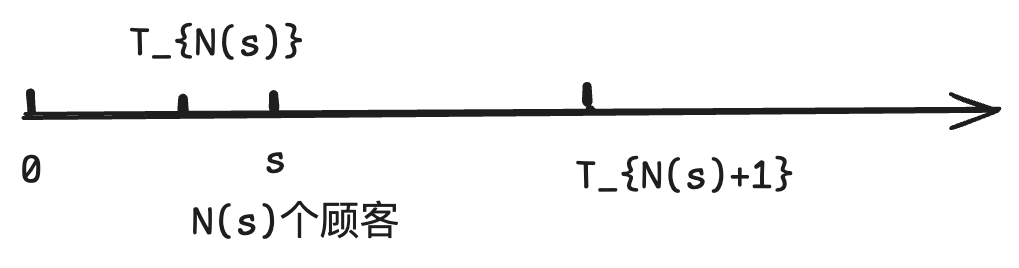
\includegraphics[width=0.35\textwidth]{figures/lem2-5.png}
        \caption{固定起始时间$s$}
        \label{fig:fixed-s}
    \end{figure}
\begin{lemma}[Lem 2.5']\label{lem:2.5}
    对固定$s\geq 0$ (图 \ref{fig:fixed-s}),
    令 $\tau_1^s:=T_{N(s)+1}-s$. $\tau_n^s:=\tau_{N(s)+n}, n\geq 2$.
    \[
    T_n^s:=\begin{cases}
        \sum_{k=1}^n\tau_k^s & n\geq 1\\
        0 & n=0
    \end{cases}
    \]
    $N^s(t):=\max\{n|T_n^s\leq t\}$. 则
    \begin{enumerate}
        \item $N^s(t)=N(t+s)-N(s)$
        \item $\forall k\geq 1, (\tau_1^s,\cdots,\tau_k^s)\ind N(s)$, 即 $\tau_k^s=\tau_k\sim \EXP(\lambda)$, $\tau_1^s, \tau_2^s, \cdots$ 相互独立
        \item $\{N^s(t)=N(t+s)-N(s),t\geq 0\}$ 为带有速率 $\lambda$ 的泊松过程, 且 $N(t+s)-N(s)\ind N(r), \forall 0\leq r\leq s,t\geq 0$
    \end{enumerate}
\end{lemma}
    \item (独立增量) 由 Lem \ref{lem:2.5} (c) 及数学归纳法
    
$n=2$, 对 $0=t_0\leq t_1<t_2$, 有 $N(t_2)-N(t_1)\ind N(t_1)=N(t_1)-N(t_0)$.
    
$n=k$, 假设对 $0=t_0\leq t_1<t_2<\cdots<t_n$, 有 $N(t_k)-N(t_{k-1}),\cdots,N(t_1)-N(t_0)$ 相互独立. 考虑 $n=k+1$, 对于第 $k+1$ 个增量 $N(t_{k+1})-N(t_k)$, 由 Lem \ref{lem:2.5} (c), 令 $s=t_k, N^{s}(t_{k+1}-t_k)\ind N(r), \forall r\leq t_k$, 因此由 Thm \ref{thm:1.3}, $N^{s}(t_{k+1}-t_k)\ind \sigma(\bigcup_{r\leq t_k}N(r))$. $\forall 1\leq j\leq k, N^{s}(t_{k+1}-t_k)\ind (N(t_j)-N(t_{j-1}))$. 又因 $\forall 1\leq j\leq k, N(t_j)-N(t_{j-1})$ 相互独立, 则 $\forall 1\leq j\leq k+1, N(t_j)-N(t_{j-1})$ 相互独立.
    \item 由 Lem \ref{lem:2.5} (a)(c) 知, 只需证 $N(t)\sim \Poi(\lambda t)$, 则有 $N(t+s)-N(s)\sim\Poi(\lambda t)$. 这是因为 Lem \ref{lem:2.5} (a)(c) 已经把 $N(t+s)-N(s)$ 表达为一个``从 $s$ 开始重新计时''的新泊松过程 $N^s(t)$, 而我们知道 $N^s(t)$ 的构造方式与原始的 $N(t)$ 完全一致, 只不过起点平移到了 $s$.
    \begin{enumerate}
        \item $\PP(N(t)=0)=\PP(T_1>t)=\PP(\tau_1>t)=e^{-\lambda t}(\lambda t)^0/(0!)$
        \item $n>0$ 时, 
        \[
        \begin{aligned}
            \PP(N(t)=n) &=\PP(T_n\leq t<T_{n+1})\\
            &=\PP(T_n\leq t<T_n+\tau_{n+1})\\
            &\xlongequal{T_n\ind \tau_{n+1}}\int_0^{+\infty}\PP(u\leq t<u+\tau_{n+1})f_{T_n}(u)du\\
            &=\int_0^{+\infty}\II_{\{u\leq t\}}\PP(\tau_{n+1}>t-u)f_{T_n}(u)du\\
            &=\int_0^t e^{-\lambda (t-u)}\lambda e^{-\lambda u}\frac{(\lambda u)^{n-1}}{(n-1)!}du\\
            &=\frac{\lambda^n e^{-\lambda t}}{(n-1)!}\int_0^t e^{\lambda u}\cdot e^{-\lambda u}u^{n-1}du\\
            &=\frac{\lambda^n e^{-\lambda t}}{(n-1)!}\cdot \frac{1}{n}\cdot u^n|_0^t=\frac{(\lambda t)^n e^{-\lambda t}}{n!}\sim \Poi(\lambda t)
        \end{aligned}
        \]
    \end{enumerate}
\end{enumerate}
\end{proof}

下面证明 Lem \ref{lem:2.5}.
\begin{proof}
\begin{enumerate}
    \item[(a)] 要证 $N^s(t)=N(t+s)-N(s)$. 
    
    $n\geq 1, T_n^s=T_{N(s)+1}-s+\tau_{N(s)+2}+\cdots +\tau_{N(s)+n}=T_{N(s)+n}-s, T_{N(s)}\leq s$
    \[
    \begin{aligned}
        N^s(t)&=\max\{n\geq 0|T_n^s\leq t\}\\
        &=\max\{n\geq 0|T_{N(s)+n}\leq t+s\}\\
        &\xlongequal{m=N(s)+n}\max\{m-N(s)\geq 0|T_m\leq t+s\}\\
        &=\max\{m\geq 0|T_m\leq t+s\}-N(s)\\
        &=N(t+s)-N(s)
    \end{aligned}
    \]
    \item[(b)] 要证明
    \begin{quote}
        $\forall k\geq 1$, \framebox{$(\tau_1^s,\cdots,\tau_k^s)\ind N(s)$}, 即 $\tau_k^s=\tau_k\sim \EXP(\lambda)$, $\tau_1^s, \tau_2^s, \cdots$ 相互独立
    \end{quote}
    实际上方框内的陈述更强, 目前无法证明, 所以只证后面的部分.
    \begin{enumerate}
        \item[(1)] $k=1$,
        \[
        \begin{aligned}
        \PP(\tau_1^s>t_1,N(s)=n) &=\PP(T_{N(s)+1}-s>t_1,N(s)=n)\\
        &=\PP(T_{n+1}>t_1+s,s\geq T_n)\\
        &=\PP(\tau_{n+1}>t_1+s-T_n, T_n\leq s)\\
        &\xlongequal{T_n\ind \tau_{n+1}}\int_0^{+\infty}\PP(\tau_{n+1}>t_1+s-u,u\leq s)f_{T_n}(u)du\\
        &=\int_0^{+\infty}\II_{\{u\leq s\}}\PP(\tau_{n+1}>t_1+s-u)f_{T_n}(u)du\\
        &\xlongequal{(*)}\int_0^{+\infty}\II_{\{u\leq s\}}\PP(\tau_{n+1}>s-u)f_{T_n}(u)du\cdot \PP(\tau_{n+1}>t_1)\\
        &=\PP(\tau_{n+1}>s-T_n,T_n\leq s)\PP(\tau_{n+1}>t_1)\\
        &=\PP(T_{n+1}>s\geq T_n)\PP(\tau_{n+1}>t_1)\\
        &=\PP(N(s)=n)\PP(\tau_{n+1}>t_1)
        \end{aligned}
        \]
        $(*)$ 处用了指数分布的无记忆性, 
        \[
        \begin{aligned}
				\PP(\tau_{n+1}>t_1+s-u)&=\PP(\tau_{n+1}>t_1+s-u|\tau_{n+1}>t_1)\cdot \PP(\tau_{n+1}>t)\\
				&=\PP(\tau_{n+1}>s-u)\cdot \PP(\tau_{n+1}>t)
				\end{aligned}
        \]
        最后关于 $n$ 求和, 
        \[
        \sum_{n\geq 0}\PP(\tau_1^s>t_1,N(s)=n)=\sum_{n\geq 0}\PP(N(s)=n)\PP(\tau_{n+1}>t_1)
        \]
        其中 $\LHS=\PP(\tau_1^s>t_1)$. 因为 $\PP(\tau_{n+1}>t_1)\xlongequal{iid}\PP(\tau_{1}>t_1)$, $\Rightarrow \RHS=\PP(\tau_{1}>t_1) \Rightarrow \tau_1^s\sim \EXP(\lambda)$. 代回, 得 $\PP(\tau_1>t_1)=\PP(\tau_1^s>t_1)$, 即 $\tau_1^s\ind N(s)$.

        注: $\PP(T_{n+1}-s>t|N(s)=n)=\PP(\tau_1^s>t|N(s)=n)=\PP(\tau_1>t)$. $\Rightarrow T_{n+1}-s\sim \EXP(\lambda)$ under $\PP(\cdot|N(t)=n)$.
        \item[(2)] $k\geq 2$时, 
        \[
        \begin{aligned}
            A_n &:=\{N(s)=n,\tau_1^s>t_1,\tau_2^s>t_2,\cdots, \tau_k^s>t_k\}\\
            &=\{T_n\leq s,T_{n+1}>t_1+s\}\cap \left\{\bigcap_{i=2}^k \{\tau_{n+i}>t_i\}\right\}
        \end{aligned}
        \]
        \[
        \begin{aligned}
            \PP(A_n) &=\PP(T_n\leq s, T_{n+1}>t_1+s)\prod_{i=2}^k \PP(\tau_{n+i}>t_i)\\
            &\xlongequal{(1)}\PP(N(s)=n)\PP(\tau_1>t_1)\prod_{i=2}^k\PP(\tau_{n+i}>t_i)
        \end{aligned}
        \]
        在概率测度意义下 $\tau_{n+i}\overset{(d)}{=}\tau_i$, 关于 $n$ 求和, $(\tau_1^s,\cdots,\tau_k^s)\overset{(d)}{=}(\tau_1,\cdots,\tau_k)$, 即 $\tau_1^s,\cdots,\tau_k^s$ 相互独立, 代回前式得 $(\tau_1^s,\cdots,\tau_k^s)\ind N(s)$.
        \item[(3)] 类似前面两步的技巧.
    \end{enumerate}
    \item[(c)] 不妨设 $0\leq t_1<\cdots<t_k$
    \[
    \begin{aligned}
        \{N^s(t_1)=m_1,\cdots,N^s(t_k)=m_k\} &=\{T_{m_1}^s\leq t_1< T_{m_1+1}^s,\cdots,T_{m_k}^s\leq t_k< T_{m_k+1}^s\}\\
        &=\left\{\sum_{i=1}^{m_1}\tau_i^s\leq t_1<\sum_{i=1}^{m_1+1}\tau_i^s,\cdots,\sum_{i=1}^{m_k}\tau_i^s\leq t_k<\sum_{i=1}^{m_k+1}\tau_i^s\right\}
    \end{aligned}
    \]
    由 (b), $\tau_i^s\sim \EXP(\lambda),\forall i\geq 0$. 由 Def \ref{def:poi-2}, $N^s(t_i),\forall i\geq 0$ 为速率 $\lambda$ 的泊松过程. 
    
    由于 $N^s(t)$ 是 $\{\tau_{N(s)+1},\tau_{N(s)+2},\cdots\}$ 的函数, $N(r),r\leq s$ 是 $\{\tau_1,\cdots,\tau_{N(r)}\}$ 的函数, 故 $N^s(t)\ind N(r),\forall r\leq s$.
\end{enumerate}
\end{proof}

\begin{proposition}
    Def \ref{def:counting-process-I} $\Rightarrow$ Def \ref{def:poi-2}
\end{proposition}

\begin{proof}
$\{N(t),t\geq 0\}$ 是计数过程, $T_n=\min\{t|N(t)\geq n\}, \tau_n=T_n-T_{n-1}$.
\begin{enumerate}
    \item $t\neq 0$, 
    \[
    N(t)=\sum_{n=1}^{\infty}\II_{\{N(t)\geq n\}}=\sum_{n=1}^{\infty}\II_{\{T_n\leq t\}}=\max\{n|T_n\leq t\}
    \]
    \item 下面只需证 $(\tau_k)_{k\geq 1}\overset{\text{iid}}{\sim}\EXP(\lambda)$
    \begin{enumerate}
        \item $k=1, \PP(\tau_1>t)=\PP(T_1>t)=\PP(N(t)=0)=e^{-\lambda t}(\lambda t)^0/(0!)=e^{-\lambda t}$, 故 $\tau_1\sim\EXP(\lambda)$.
        \item 考察 $(T_1,T_2)$, 支撑集为 $S=\{(x_1,x_2)\in \RR^2|0<x_1<x_2\}$. 下面需要找到 $(T_1,T_2)$ 的联合密度分布函数. 
        
        设 $0<r_1<t_1<r_2<t_2$
        \begin{figure}[H]
            \centering
            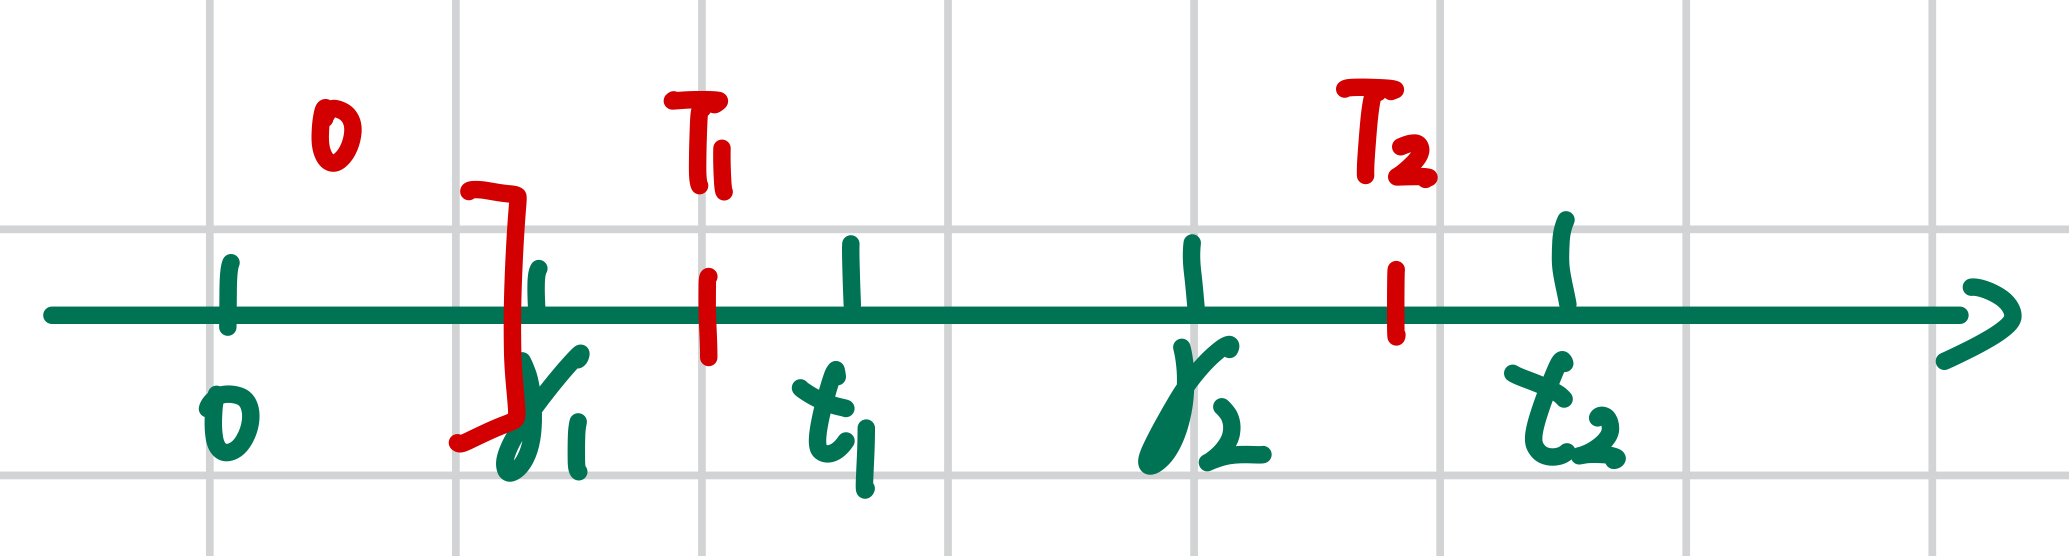
\includegraphics[width=0.35\textwidth]{figures/note-p102.png}
        \end{figure}
        \[
        \begin{aligned}
            &\PP(r_1\leq T_1<t_1,r_2\leq T_2<t_2) \\
            =&\PP(N(r_1)=0,N(r_2)-N(t_1)=0,N(t_1)-N(r_1)=1,N(t_2)-N(r_2)\geq 1)\\
            =&e^{-\lambda r_1}\cdot e^{-\lambda (r_2-t_1)}\cdot e^{-\lambda (t_1-r_1)}\cdot \frac{\lambda (t_1-r_1)}{1!}\cdot [1-e^{-\lambda (t_2-r_2)}]\\
            =&\lambda (t_1-r_1)[e^{-\lambda r_2}-e^{-\lambda t_2}]=\lambda\int_{r_1}^{t_1}dx_1\int_{r_2}^{t_2}\lambda e^{-\lambda x_2}dx_2
        \end{aligned}
        \]
        $N(t_2)-N(r_2)\geq 1$ 是因为要求第二个事件 $T_2$ 必须落在 $[r_2,t_2)$ 内, 但并不限制该区间内后续事件的数量. 联合密度函数 $\lambda^2 e^{-\lambda x_2}$ 在区域 $S$ (即 $0<x_1<x_2$) 上, 所以 $f_{(T_1,T_2)}(x_1,x_2)=\lambda^2 e^{-\lambda x_2}\II_{\{(x_1,x_2)\in S\}}$.
        \[
        \PP(\tau_1>t_1,\tau_2>t_2)=\PP(\tau_1>t_1,T_2-T_1>t_2)=\int_{x_1>t_1}\int_{x_2-x_1>t_2}\lambda^2 e^{-\lambda x_2}dx_2 dx_1=e^{-\lambda (t_1+t_2)}
        \]
        又 $\PP(\tau_1>t_1)=e^{-\lambda t_1}$, 所以 $\tau_2\sim \EXP(\lambda)$ 且 $\tau_1\ind \tau_2$. 对 $k\geq 3$ 同理.
    \end{enumerate}
\end{enumerate}
\end{proof}

\begin{definition}[Def \ref{def:counting-process-I} 推广, 非齐次的泊松过程]
    称计数过程 $\{N(t),t\geq 0\}$ 为一个速率为 $\lambda(r)$ 的非齐次泊松过程, 若
    \begin{enumerate}
        \item $N(0)=0$
        \item 独立增量性
        \item 增量的分布
        \[
        N(t+s)-N(s)\sim \Poi\left(\int_s^{t+s}\lambda(r)dr\right)
        \]
    \end{enumerate}
\end{definition}

\begin{proposition}
    非齐次泊松过程的到达间隔时间列 $\tau_1,\tau_2,\cdots$ 不再服从指数分布, 不再相互独立.
\end{proposition}
\begin{proof}
    同上计算联合分布即可.
\end{proof}
\newpage
\subsection{复合泊松过程}

\begin{definition}
    $\{N(t),t\geq 0\}$ 是一个泊松过程, $\{Y_i\}_{i\geq 1}$ 独立同分布且 $\{Y_i\}_{i\geq 1}\ind (N(t))_{t\geq 0}$. 令
    \[
    S(t):=\begin{cases}
        \sum_{i=1}^{N(t)}Y_i & N(t)\neq 0\\
        0 & N(t)=0
    \end{cases}
    \]
    则 $\{S(t)\}_{t\geq 0}$ 称为一个复合泊松过程.
\end{definition}

\begin{theorem}
    $\{Y_i\}_{i\geq 1}$ 为独立同分布 r.v. 列, $N$ 为取非负整数值的 r.v., \framebox{$\{Y_i\}_{i\geq 1}\ind N$}. 令
    \[
    S=\begin{cases}
        \sum_{i=1}^N Y_i & N\neq 0\\
        0 & N=0
    \end{cases}
    \]
    则
    \begin{enumerate}
        \item $\EE S=\EE N\cdot \EE Y_i$
        \item $\Var (S)=\EE N \Var(Y_i)+\Var(N)(\EE Y_i)^2$
        \item 特别地, 若 $N\sim \Poi(\lambda)$, 则 $\EE S=\lambda\EE Y_i,\Var(S)=\lambda[\Var(Y_i)+(\EE Y_i)^2]=\lambda \EE Y_i^2$.
    \end{enumerate}
\end{theorem}
注:
\begin{enumerate}
    \item 若 $N=n$ 非随机, 则 $\EE S=n\EE Y_i$
    \item 若 $N=n$ 非随机, $\Var(S)=n\Var(Y_i)$. 若 $Y_i$ 非随机, $\Var(S)=\Var(Y\cdot N)=Y^2\Var(N)$.
\end{enumerate}

\begin{proof}
    \begin{enumerate}
        \item 由重期望公式\eqref{eq:double-exp}, 
        \[
        \EE S=\EE(\EE(S|N))=\EE\left[\sum_{n\geq 0}\EE(S|N=n)\II_{\{N=n\}}\right]=\sum_{n\geq 0}\EE(S|N=n)\PP(N=n)
        \]
        其中 $\sum_{n\geq 0}\EE(S|N=n)\II_{\{N=n\}}$ 为一个离散随机变量. $\EE(S|N=n)$ 是一个数, 不具有随机性.
        \[
        \EE(S|N=n)=\EE\left(\sum_{i=1}^n Y_i|N=n\right)\xlongequal{\{Y_i\}\ind N}\EE\left(\sum_{i=1}^n Y_i\right)=n\EE Y_i
        \]
        所以 $\EE S=\EE N\EE Y_i$.
        \item $\EE(S^2|N=n)=\EE[\sum_{i=1}^n Y_i]^2=\Var(\sum_{i=1}^n Y_i)+[\EE \sum_{i=1}^n Y_i]^2=n\Var(Y_i)+n^2[\EE Y_i]^2$. $\EE S^2=\EE N\cdot \Var(Y_i)+\EE N^2\cdot (\EE Y_i)^2$. $\Var(S)=\EE S^2-(\EE S)^2=\EE N\Var(Y_i)+\Var(N)(\EE Y_i)^2$
    \end{enumerate}
\end{proof}
\newpage
\subsection{泊松过程的变换}
\begin{enumerate}
    \item 稀释 (thining): 把一个泊松过程拆分成若干个独立的泊松过程
    \item 叠加 (superposition): 把若干个独立的泊松过程合并成一个泊松过程
\end{enumerate}

\subsubsection{稀释/可分解性}

\begin{theorem}
    $(N(t))_{t\geq 0}\sim \PoiP(\lambda)$, $(Y_i)_{i\geq 1}$ 为 iid 的离散随机变量列, $(Y_i)_{i\geq 1}\ind (N(t))_{t\geq 0}$. $\PP(Y_i=j)=p_j,1\leq j\leq m$. 令
    \[
    N_j(t):=\sum_{i=1}^{N(t)}\II_{\{Y_i=j\}}, 1\leq j\leq m
    \]
    约定 $\sum_a^b(\cdot)=0, b<a$. 则
    \begin{enumerate}
        \item $N(t)=\sum_j N_j(t)$
        \item $\{N_j(t),t\geq 0\},1\leq j\leq m$ 为相互独立的泊松过程, 且速率分别为 $\lambda p_j$
    \end{enumerate}
\end{theorem}
注: $m=2$时, $\PP(Y_i=1)=p,\PP(Y_i=2)=1-p$. e.g. $N_1(t)$: $[0,t]$之间性别1的顾客数; $N_2(t)$: $[0,t]$之间性别2的顾客数.

\begin{proof}
下面证明 $N_1(t)$ 服从泊松过程, 且速率为 $\lambda p_1$. 由 Def \ref{def:counting-process-I}, 依次证明三个性质.
\begin{enumerate}
    \item $N(0)=N_1(0)+N_2(0)=0$
    \item 接着证明 $N_1(t)$ 的增量服从泊松分布, 即 $\forall s\geq 0,t>0, N_1(t+s)-N(s)\sim \Poi(\lambda p_1 t)$.
    
    (Step 1) Claim: $N_1(t)\sim\Poi(\lambda pt),p_1=p$
    \begin{equation}
        \PP(N_1(t)=n)=\sum_{m\geq 0}\PP(N_1(t)=n|N(t)=n+m)\PP(N(t)=n+m)
        \label{eq:p105}
    \end{equation}
    $(Y_i)_{i\geq 1}\overset{\text{iid}}{\sim}(N(r))_{r\geq 0}$, $\Rightarrow (\II_{\{Y_i=1\}})_{i\geq 1}\ind (N(r))_{r\geq 0}$. 所以
    \begin{equation}
        \sum_{i=1}^{n+m}\II_{\{Y_i=1\}}=n\ind (N(r))_{r\geq 0}
        \label{eq:p106-2}
    \end{equation}
    由 \eqref{eq:p106-2},
    \begin{equation}
        \PP\left(\sum_{i=1}^{N(t)}\II_{\{Y_i=1\}}=n|N(t)=n+m\right)\xlongequal{\ind}\PP\left(\sum_{i=1}^{n+m}\II_{\{Y_i=1\}}=n\right)\xlongequal{\text{iid}}\binom{n+m}{n}p^n(1-p)^m
        \label{eq:p106-3}
    \end{equation}
    其中 $\II_{\{Y_i=1\}}\sim\Ber(p)$. 将 \eqref{eq:p106-3} 代回 \eqref{eq:p105}, 得
    \[
    \begin{aligned}
        \PP(N_1(t)=n) &=\sum_{m\geq 0}\frac{(n+m)!}{n!m!}p^n(1-p)^m e^{-\lambda t}\frac{(\lambda t)^{n+m}}{(n+m)!}\\
        &=\frac{(\lambda pt)^n}{n!}e^{-\lambda t}\sum_{m\geq 0}\frac{(\lambda t(1-p))^m}{m!}\\
        &=\frac{(\lambda pt)^n}{n!}e^{-\lambda t}e^{\lambda t(1-p)}\\
        &=e^{-\lambda pt}\frac{(\lambda pt)^n}{n!}
    \end{aligned}
    \]
    (Step 2)
    \[
    N_1(t+s)-N_1(s)=\sum_{i=N(s)+1}^{N(t+s)}\II_{\{Y_i=1\}}=\sum_{\tilde{i}=1}^{N(t+s)-N(s)}\II_{\{Y_{N(s)+\tilde{i}}=1\}}
    \]
    由 (Step 1) 的证明步骤知, 需要条件 $(Y_{N(s)+i})_{i\geq 1}\ind (N(t+s)-N(s))_{t\geq 0}$ 使得 $N(t+s)-N(s)\sim \Poi(\lambda pt)$
    \begin{lemma}\label{lem:p106}
        令 $Y_i^s:=Y_{N(s)+i}, N_1^s(t):=\sum_{i=1}^{N^s(t)}\II_{\{Y_i^s=1\}}$, 则
        \begin{enumerate}
            \item[(a)] $N_1^s(t)=N_1(t+s)-N_1(s)$
            \item[(b)] $1^{\circ} (Y_i^s)_{i\geq 1}$, iid, $Y_i^s\overset{(d)}{=}Y_i$
            
            $2^{\circ} (Y_i^s)_{i\geq 1}\ind (N^s(t))_{t\geq 0}$
            \item[(c)] $N_1^s(t)\sim \Poi(\lambda pt)$
        \end{enumerate}
    \end{lemma}
    \begin{proof}
        \begin{enumerate}
        \item[(a)] 因为 $N^s(t)=N(t+s)-N(s)$
        \[
        \begin{aligned}
N_1^s(t)&=\sum_{i=1}^{N^s(t)}\II_{\{Y_i^s=1\}}=\sum_{i=1}^{N(t+s)-N(s)}\II_{\{Y_{N(s)+i}=1\}}\\
&\xlongequal{\tilde{i}=N(s)+i}\sum_{\tilde{i}=N(s)+1}^{N(t+s)}\II_{\{Y_{\tilde{i}}=1\}}=N_1(t+s)-N_1(s)
\end{aligned}
        \]
        \item[(b)] 
        		 \begin{enumerate}
            \item[$1^{\circ}$] 牢记 $(Y_i)_{i\geq 1}$ 是 iid 的. 注意到 $Y_{N(s)+i}$ 中 $N(s)$ 是随机的, 要将其固定才能用 $(Y_i)_{i\geq 0}$ 的性质.
            \[
            \begin{aligned}
                \PP(Y_{N(s)+i_1}=j_1, Y_{N(s)+i_2}=j_2)&= \sum_{n\geq 0}\PP(Y_{N(s)+i_1}=j_1,Y_{N(s)+i_2}=j_2|N(s)=n)\PP(N(s)=n)\\
                &\xlongequal{\text{iid}}\sum_{n\geq 0}\PP(Y_{i_1}=j_1)\PP(Y_{i_2}=j_2)\PP(N(s)=n)\\
                &=\PP(Y_{i_1}=j_1)\PP(Y_{i_2}=j_2)
            \end{aligned}
            \]
            故 $(Y_{i_1}^s,Y_{i_2}^s)\overset{(d)}{=}(Y_{i_1},Y_{i_2})$, $(Y_i^s)_{i\geq 1}$ 相互独立
            \item[$2^{\circ}$] $Y^s_i$ 中存在 $N(s)$, $N^s(t)=N(t+s)-N(s)$ 中也存在 $N(s)$, 先将其固定. 
            \[
            \begin{aligned}
     &\quad\PP(Y_i^s=j|N^s(t_1)=m_1,\cdots,N^s(t_k)=m_k)\\     
&=\sum_{m\geq 0}\PP(Y_{N(s)+i}=j|N^s(t_1)=m_1,\cdots,N^s(t_k)=m_k,N(s)=m)\PP(N(s)=m)\\
&\xlongequal{Y\ind N(\cdot)}\PP(Y_{m+i}=j)\sum_{m\geq 0}\PP(N(s)=m)\\
&\xlongequal{1^{\circ}}\PP(Y_i^s=j)
\end{aligned}
            \]
            \end{enumerate}
				\item[(c)] 由 (Step 1) 步骤, (b) 独立性满足时, $N_1(t+s)-N_1(s)\sim \Poi(\lambda pt)$. 由 (a), $N_1(t+s)-N_1(s)$ 就是 $N_1^s(t)$, 所以 $N_1^s(t)\sim \Poi(\lambda pt)$.
        \end{enumerate}
    \end{proof}
    由 Lem \ref{lem:p106} (c) 知, $N_1(t+s)-N_1(s)\sim \Poi(\lambda pt)$. 
    
    \item (独立增量性) $0=t_0<t_1<t_2,0=n_0<n_1<n_2$. 要证 $\PP(N_1(t_j)-N_1(t_{j-1})=m_j,1\leq j\leq 2)=\PP(N_1(t_1)-N_1(t_0)=m_1)\cdot\PP(N_1(t_2)-N_1(t_1)=m_2)$. 由于 $N(t)$ 随机, 要先将其固定.
        \begin{equation}
        \begin{aligned}
            A&:=\PP(N_1(t_j)-N_1(t_{j-1})=m_j,1\leq j\leq 2|(N(t_1),N(t_2))=(n_1,n_2))\\
            &=\PP\left(\sum_{i=N(t_{j-1})+1}^{N(t_j)}\II_{\{Y_i=1\}}=m_j,1\leq j\leq 2\bigg|(N(t_1),N(t_2))=(n_1,n_2)\right)\\
            &\xlongequal{\II_{\{Y_i=1\}}\ind (N(t))_{t\geq 0}}\PP\left(\sum_{i=n_{j-1}+1}^{n_j}\II_{\{Y_i=1\}}=m_j,1\leq j\leq 2\right)\\
            &=\prod_{j=1}^2 \PP\left(\sum_{i=n_{j-1}+1}^{n_j}\II_{\{Y_i=1\}}=m_j\right)
        \end{aligned}
        \label{eq:p90-A}
        \end{equation}
        	最后一个等式成立是因为, $j=1,2$ 时, 求和的区间分别为 $[n_0+1,n_1],[n_1+1,n_2]$, 因此相互独立.
        	
        	因为 $(N(t))_{t\geq 0}$ 为泊松过程, 由其独立增量性,
        	\begin{equation}
        	\begin{aligned}
        	\PP(N(t_1)=n_1,N(t_2)=n_2)&=
        	\PP(N(t_1)=n_1,N(t_2)-N(t_1)=n_2-n_1)\\
        	&=\PP(N(t_1)=n_1)\cdot \PP(N(t_2)-N(t_1)=n_2-n_1)
        	\end{aligned}
        	\label{eq:p90-indep}
        	\end{equation}
由 \eqref{eq:p90-A} 和 \eqref{eq:p90-indep},
        \[
        \begin{aligned}
        &\PP(N_1(t_j)-N_1(t_{j-1})=m_j,1\leq j\leq 2)\\
            =&\sum_{n_2\geq n_1\geq 0}A\cdot \PP(N(t_1)=n_1,N(t_2)=n_2)\\
            =&\sum_{n_2\geq n_1\geq 0}\prod_{j=1}^2\PP\left(\sum_{i=n_{j-1}+1}^{n_j}\II_{\{Y_i=1\}}=m_j\right)\cdot \PP(N(t_1)-N(t_0)=n_1)\cdot \PP(N(t_2)-N(t_1)=n_2-n_1)
				\end{aligned}
				\tag{$*1$}
				\]
				令 $\tilde{i}=i+n_{j-1}$.
				\[
				\begin{aligned}
            (*1)&=\sum_{n_2\geq n_1\geq 0}\prod_{j=1}^2\PP\left(\sum_{\tilde{i}=1}^{n_j-n_{j-1}}\II_{\{Y_{\tilde{i}}^{t_{j-1}}=1\}}=m_j\right)\PP(\underbrace{\displaystyle N(t_j)-N(t_{j-1})}_{N^{t_{j-1}}(t_j-t_{j-1})}=n_j-n_{j-1})\\
            &\xlongequal{Y_i\ind N}\sum_{n_2\geq n_1\geq 0}\prod_{j=1}^2 \PP\left(\sum_{i=1}^{N^{t_{j-1}}(t_j-t_{j-1})}\II_{\{Y_i^{t_{j-1}}=1\}}=m_j, N(t_j)-N(t_{j-1})=n_j-n_{j-1}\right)\\
            &=\sum_{n_2\geq n_1\geq 0}\prod_{j=1}^2 \PP(N_1^{t_{j-1}}(t_j-t_{j-1})=m_j, N(t_j)-N(t_{j-1})=n_j-n_{j-1})
            \end{aligned}
            \tag{$*2$}
            \]
            把累乘展开, 再用示性函数的技巧把一个$n_1,n_2$有制约关系的求和变成两个单独的求和, 依次消去原本固定 $N(t)$ 用的 $N(t_2)-N(t_1)=n_2-n_1$ 和 $N(t_1)=n_1$.
            \[
            \begin{aligned}
            (*2)&=\sum_{n_1\geq 0}\sum_{n_2\geq 0}\II_{\{n_2\geq n_1\}}\cdot \PP(N_1(t_1)=m_1,N(t_1)=n_1)\cdot \PP(N_1(t_2)-N_1(t_1)=m_2,N(t_2)-N(t_1)=n_2-n_1)\\
            &=\sum_{n_1\geq 0}\PP(N_1(t_1)=m_1,N(t_1)=n_1)\PP(N_1(t_2)-N_1(t_1)=m_2)\\
            &=\PP(N_1(t_1)=m_1)\cdot \PP(N_1(t_2)-N_1(t_1)=m_2)
        \end{aligned}
        \]
        也就是
        \[
        \PP(N_1(t_j)-N_1(t_{j-1})=m_j,1\leq j\leq 2)=\PP(N_1(t_1)=m_1)\cdot \PP(N_1(t_2)-N_1(t_1)=m_2)
        \]
        所以 $N_1(t_j)-N_1(t_{j-1}),j=1,2$ 相互独立.
\end{enumerate}
\end{proof}

\subsubsection{叠加}

\begin{theorem}
    $\{N_j(t),t\geq 0\}\sim \PoiP(\lambda_j), 1\leq j\leq k$, 相互独立.
    \begin{equation}
        \left(\sum_{j=1}^k N_j(t)\right)_{t\geq 0}\sim \Poi\left(\sum_{j=1}^k\lambda_j\right)
    \end{equation}
\end{theorem}

\begin{proof}
    $k=2$, 令 $N(t)=N_1(t)+N_2(t)$.
    \begin{enumerate}
        \item $N(0)=0$
        \item $(N_1(t))_{t\geq 0}\ind (N_2(t))_{t\geq 0}$. 故 $\forall 0=t_0<t_1<\cdots<t_n$, 有 $(N_1(t_1),\cdots,N_1(t_n))\ind (N_2(t_1),\cdots,N_2(t_n))$.
        \[
        \begin{aligned}
            &(N_1(t_1),N_1(t_2)-N_1(t_1),\cdots,N_1(t_n)-N_1(t_{n-1}))\\
            &\ind (N_2(t_1),N_2(t_2)-N_2(t_1),\cdots,N_2(t_n)-N_2(t_{n-1}))
        \end{aligned}
        \]
        $\forall 1\leq j\leq n, N_1(t_j)-N_1(t_{j-1}),N_2(t_j)-N_2(t_{j-1})$ 相互独立.
        
        $\Rightarrow (N_1(t_j)-N_1(t_{j-1}), N_2(t_j)-N_2(t_{j-1})), 1\leq j\leq n$ 相互独立
        
        $\therefore N(t_j)-N(t_{j-1})=(N_1(t_j)-N_1(t_{j-1}))+(N_2(t_j)-N_2(t_{j-1})), 1\leq j\leq n$ 相互独立
        \item $N(t+s)-N(s)=(N_1(t+s)-N_1(s))+(N_2(t+s)-N_2(s))\sim \Poi(\lambda_1 t+\lambda_2 t)$
    \end{enumerate}
\end{proof}

\begin{example}[Durrett Exa 2.12, A Poisson Race]
    Given a Poisson process of red arrivals with rate $\lambda$ and an independent Poisson process of green arrivals with rate $\mu$, what is the probability that we will get $6$ red arrivals before a total of $4$ green ones?
\end{example}
\begin{proof}[解]
    $(N_r(t))_{t\geq 0}\sim\PoiP(\lambda), (N_g(t))_{t\geq 0}\sim \PoiP(\mu)$ 相互独立, 问: $\PP(T_4^g>T_6^r)$?

    $N(t)=N_r(t)+N_g(t)\sim \PoiP(\lambda +\mu)$.
    
    (Step 1) $A=\{T_4^g>T_6^r\}, B=\{[0,T_9]\text{之间至少有}6\text{个红队队员}\}$. Claim: $A=B$.
        \begin{enumerate}
            \item ($B\st A$) $[0,T_9]$ 之间红 $\geq 6$ 个, 绿 $\leq 3$ 个. $T_6^r\leq T_9\leq T_4^g$.
            \item ($A\st B, B^c\st A^c$) $[0,T_9]$ 之间红 $\leq 5$ 个, 绿 $\geq 4$ 个. $T_6^r\geq T_9\geq T_4^g$.
        \end{enumerate}
        以上用叠加. 便于下面使用稀释的定理.
        
  (Step 2) 将 $(N(t))_{t\geq 0}$ 按照 $(Y_i)_{i\geq 1}$ 稀释. 其中 $(Y_i)_{i\geq 1}$ iid 且 $(Y_i)_{i\geq 1}\ind (N(t))_{t\geq 0}$, $\PP(Y_i=r)=\lambda/(\lambda+\mu)$. 得到
        \begin{enumerate}
            \item $\tilde{N}_r(t)=\sum_{i=1}^{N(t)}\II_{\{Y_i=r\}}\sim\PoiP(\lambda)$. $\tilde{N}_g(t)=\sum_{i=1}^{N(t)}\II_{\{Y_i=g\}}\sim\PoiP(\mu)$. 两者相互独立.
            \item $N(t)=\tilde{N}_r(t)+\tilde{N}_g(t)$
        \end{enumerate}
        于是 $(T_4^g, T_6^r)\overset{(d)}{=}(\tilde{T}_4^g,\tilde{T}_6^r)$. 由 $\{T_n\leq t\}=\{N(t)\geq n\}$, 将 $T$ 改写成 $N$, 则 $T,\tilde{T}$ 同分布, $N,\tilde{N}$ 同分布.
        \[
        \begin{aligned}
            \PP(A) &=\PP(\tilde{T}_4^g>\tilde{T}_6^r)\\
            &=\PP(B)=\PP(\tilde{N}_r(T_9)\geq 6)\\
            &=\PP\left(\sum_{i=1}^{N(T_9)=9}\II_{\{Y_i=r\}}\geq 6\right)\\
            &=\sum_{k=6}^9\binom{9}{k}\left(\frac{\lambda}{\lambda+\mu}\right)^{k}\left(\frac{\mu}{\lambda+\mu}\right)^{n-k}
        \end{aligned}
        \]
\end{proof}
注: 为什么不用 $N_r(t),N_g(t)$, 而是先叠加再稀释构造 $\tilde{N}_r(t),\tilde{N}_g(t)$? 若直接用 $N_r(t),N_g(t)$, 则 $T_6^r\sim\Gamma(6,\lambda), T_4^g\sim\Gamma(4,\mu)$, 要计算
\[
\PP(T_4^g>T_6^r)=\int_0^{\infty}f_{T_6^r}(t)\cdot \PP(T_4^g>t)dt
\]
非常复杂. 而转化成计算 $\PP(\tilde{T}_4^g>\tilde{T}_6^r)$ 则将问题离散化.

\subsubsection{条件分布}

\begin{theorem}[到达时刻的条件分布]\label{thm:2.14}
    $\{N(t),t\geq 0\}\sim\Poi(\lambda), \{T_k,k\geq 1\}$ 为其的到达时刻序列, 则 $\forall n\geq 1$, 有
    \begin{equation}
        (T_1,\cdots,T_n|N(t)=n)\overset{(d)}{=}(V_1,\cdots,V_n)
        \label{eq:p111-1}
    \end{equation}
    其中 $V_1\leq V_2\leq \cdots\leq V_n$ 是 $\{U_k,1\leq k\leq n\}\overset{\text{iid}}{\sim}\Uni[0,t]$ 的重排.
\end{theorem}

\begin{proof}
思路: 分别写出 $(T_1,\cdots,T_n|N(t)=n)$ 和 $(V_1,\cdots,V_n)$ 的分布函数.

    Claim: 
    \begin{equation}
        f_{(T_1,\cdots,T_n|N(t)=n)}(x_1,\cdots,x_n)=\frac{n!}{t^n}\cdot\II_{\{0<x_1<x_2<\cdots<x_n\}}
        \label{eq:p111-2}
    \end{equation}
    为了让 $T_1=t_1, T_2=t_2,\cdots,T_n=t_n,N(t)=n$, 则 $\tau_1=t_1,\tau_2=t_2-t_1,\cdots,\tau_n=t_n-t_{n-1},\tau>t-t_n$.
    \[
        f_{T_1,\dots,T_n}(x_1,\dots,x_n) = \prod_{k=1}^n\lambda e^{-\lambda \tau_k}\cdot e^{-\lambda(t-t_n)}= \lambda^n e^{-\lambda t}
    \]
    \[
        \PP(N(t)=n) = \frac{(\lambda t)^n}{n!} e^{-\lambda t}
    \]
    相除得到 \eqref{eq:p111-2}.
    \begin{equation}
        f_{(V_1,\cdots,V_n)}(y_1,\cdots,y_n)=\frac{n!}{t^n}\cdot\II_{\{0<y_1<y_2<\cdots<y_n\}}
        \label{eq:p111-3}
    \end{equation}
    $S_n:=\{\sigma:\{1,2,\cdots,n\}\to\{1,2,\cdots,n\}|\sigma\text{双射}\}$, $A_k:=(x_k,y_k],k=1,2,\cdots,n$. 
    
    其中$0<x_1<y_1<x_2<y_2<\cdots<x_n<y_n\leq t$.
    \[
    \begin{aligned}
        \PP(V_1\in A_1,\cdots,V_n\in A_n) &=\sum_{\sigma\in S_n}\PP(V_1\in A_1,\cdots,V_n\in A_n|U_1\in A_{\sigma(1)},\cdots,U_n\in A_{\sigma(n)})\\
        &\quad \times \PP(U_1\in A_{\sigma(1)},\cdots,U_n\in A_{\sigma(n)})\\
        &\xlongequal{\text{iid}}\sum_{\sigma\in S_n}\PP(U_1\in A_{\sigma(1)})\cdots \PP(U_n\in A_{\sigma(n)})\\
        &=n!\prod_{k=1}^n \left(\frac{y_k-x_k}{t}\right)
    \end{aligned}
    \]
    求导, 即得 \eqref{eq:p111-3}.
\end{proof}

\begin{theorem}
    若 $0<s<t,0\leq m\leq n$, 则
    \begin{equation}
        \PP(N(s)=m|N(t)=n)=\binom{n}{m}\left(\frac{s}{t}\right)^m\left(1-\frac{s}{t}\right)^{n-m}
        \label{eq:p111-4}
    \end{equation}
    即 $(N(s)|N(t)=n)\sim \Bi(n,\frac{s}{t})$
\end{theorem}

\begin{proof}
    用示性函数表示离散随机变量 $N(s)=\max\{n|T_n\leq s\}=\sum_{k=1}^{N(s)}\II_{\{T_k\leq s\}}=\sum_{k=1}^{N(t)}\II_{\{T_k\leq s\}}$.
    \[
    \begin{aligned}
        \PP(N(s)=m|N(t)=n) &=\PP\left(\sum_{k=1}^{N(t)}\II_{\{T_k\leq s\}}=m|N(t)=n\right)\\
        &\overset{\text{(i)}}{=}\PP\left(\sum_{k=1}^n\II_{\{V_k\leq s\}}=m\right)\\
        &\overset{\text{(ii)}}{=}\binom{n}{m}\left(\frac{s}{t}\right)^m\left(1-\frac{s}{t}\right)^{n-m}
    \end{aligned}
    \]
    其中 
    
    (i) 由 Thm \ref{thm:2.14}, $(\II_{\{T_1\leq s\}}, \cdots,\II_{\{T_n\leq s\}}|N(t)=n)\xlongequal{(d)}(\II_{\{V_1\leq s\}},\cdots,\II_{\{V_n\leq s\}})$. 
    
    (ii) 由 $\II_{\{V_k\leq s\}}\sim \Ber(s/t)$ 相互独立.
\end{proof}
\newpage

\pagebreak

\section{更新过程}
\subsection{定义}

\begin{definition}
    设 $\{\tau_k,k\geq 1\}\iidsim F(\cdot)$ 为非负随机变量列, 即 $\PP(\tau_1\leq t)=F(t)$, 其中 $F(0)=\PP(\tau_1\leq 0)=0$ 则 $0<\EE \tau_1<\infty$. 令 $T_n=\sum_{k=1}^n\tau_k,n\geq 1,T_0=0$, 则称由 $N(t)=\max\{n|T_n\leq t\}, t>0$ 定义的计数过程为更新过程.  
\end{definition}
注:
\begin{enumerate}
    \item $\tau_k$: 第$k$个灯泡的寿命/更新时间间隔序列
    \item $T_n$: 第$n$个灯泡损坏的时刻/第$n$次更新的时刻
    \item $N(t)$: $[0,t]$ 中灯泡的损坏个数/更新的次数
    \[
    N(t)=\sum_{n=1}^{\infty}n\II_{\{N(t)=n\}}=\sum_{n=1}^{\infty}n\II_{[T_n,T_{n+1})}(t)
    \]
\end{enumerate}

\begin{lemma}\label{lem:p113-lem1}
    $\forall t\geq 0$, 有 $N(t)<\infty$ a.s. (almost surely/几乎必然/几乎处处), 即存在零测集 $\tilde{\Omega}^c,\stt \forall \omega \in \tilde{\Omega}$, 有 $N(t)(\omega)<+\infty$, 即 \framebox{$\PP(N(t)<+\infty)=1$}.

    注: 这样写的前提是 $N(t)<\infty$ 是可测集. 因为 $N(t)$ 是随机变量, 该前提成立.
\end{lemma}

注:
\[
    \PP(N(t)=+\infty)=\lim_{n\to +\infty}\PP(\underbrace{N(t)\geq n}_{\iff T_n\leq t})=\lim_{n\to +\infty}F^{*n}(t)
\]
其中 $F^{*n}$ 为 $F$ 的 $n$ 重卷积.

\begin{theorem}[强大数定律]
    $\{X_k,k\geq 1\}$ iid, $\EE |X_1|<+\infty$, 令 $S_n=\sum_{k=1}^nX_k$, 则 $\displaystyle \frac{S_n}{n}\as{n} \EE X_1$, 即存在零测集 $\displaystyle \tilde{\Omega}^c,\stt \forall \omega \in \tilde{\Omega}$, 有 $\displaystyle \lim_{n\to\infty}\frac{S_n}{n}(\omega)= \EE X_1$, 即 $\displaystyle \PP\left(\lim_{n\to\infty}\frac{S_n}{n}=\EE X_1\right)=1$.
\end{theorem}
注: 可列 r.v. 的极限也是 r.v., 而不可列 r.v. 的极限不一定是 r.v.

\begin{proof}[证明Lem \ref{lem:p113-lem1}]
    应用SLLN知, $T_n/n\as{n}\EE \tau_1\in (0,+\infty]$.

    存在零测集 $\tilde{\Omega}^c,\stt \forall \omega \in \tilde{\Omega}$, 有
    \[
    \lim_{n\to\infty}\frac{T_n}{n}(\omega)=\EE \tau_1
    \]
    $\because \EE \tau_1>0, T_n(\omega)\approx n\EE \tau_1$. $\therefore 0\leq T_n\uparrow\Rightarrow \forall \omega\in\tilde{\Omega}$, 有 $\lim_{n\to +\infty}T_n(\omega)=+\infty$. 
    
    $N_t(\omega)=\max\{n\geq 0|T_n(\omega)\leq t\}$, 由于 $T_n(\omega)\to +\infty, \therefore \forall \omega\in\tilde{\Omega},\forall t\geq 0$, 至多只有有限个 $n$, 使 $T_n(\omega)\leq t$, 即至多只有有限个 $T_n(\omega)$ 落在 $[0,t]$ 上.

    $\Rightarrow \forall \omega\in\tilde{\Omega},\forall t\geq 0, N_t(\omega)<+\infty$, $\Rightarrow \forall t\geq 0,N(t)<+\infty$ (a.s.)
\end{proof}
\newpage
\subsection{极限定理}
\subsubsection{更新过程的大数定律}

先讲一下过程本身的极限.
\begin{lemma}\label{lem:p114-lem2}
    \[
    N(t)\as{t} +\infty
    \]
    即存在零测集 $\tilde{\Omega}^c,\stt \forall \omega \in \tilde{\Omega}$, 有 $\lim_{t\to\infty}N(t,\omega)=+\infty$. 即 $\PP(\lim_{t\to\infty}N(t)=+\infty)=1$.

    注: $N(t)$ 非可列 r.v., 但 $\lim_{t\to\infty}N(t)$ 仍为 r.v., 因为 $N(t)$ 关于 $t$ 右连左极 (\textit{cadlag}), 即右连续存在, 左极限存在.
\end{lemma}

\begin{proof}
考察 $\omega\in\{\limit{t}N(t)<\infty\}$.

$\lim_{t\to\infty}N(t)<+\infty$, $N(t)$关于$t\uparrow$ 单调上升. $\Rightarrow \exists M>0,\stt \forall t\geq 0, N(t)\leq M\Rightarrow T_M\leq t< T_{M+1}$

又因 $\Rightarrow \forall t\geq 0,T_{M+1}>t$, 故$\Rightarrow T_{M+1}=+\infty$.
    \[
    \begin{aligned}
        \PP(\limit{t}N(t)<+\infty)&\leq \PP(\exists n,T_n=+\infty)=\PP(\exists n,\tau_n=+\infty)\\
        &\leq \sum_{n\geq 1}\PP(\tau_n=+\infty)=\sum_{n\geq 1}(1-\PP(\tau_n<+\infty))\\
        &=\sum_{n\geq 1}(1-\limit{t_n}F(t_n))=0
    \end{aligned}
    \]
\end{proof}

\begin{theorem}[更新过程的LLN]\label{thm:p114-thm3.1}
    \[
    \frac{N(t)}{t}\as{t}\frac{1}{\EE\tau_1}
    \]
    即 $\PP(\limit{t}N(t)/t=1/\EE\tau_1)=1$, (因$N(t)/t$ cadlag). 
\end{theorem}

\begin{proof}
    当$N(t)<+\infty$时, $T_{N(t)}\leq t<T_{N(t)+1}$

    当$0<N(t)<+\infty$时,
    \[
    \begin{aligned}
        \boxed{\frac{T_{N(t)}}{N(t)}}\leq \frac{t}{N(t)}&<\frac{T_{N(t)+1}}{N(t)}\\
        &=\boxed{\frac{T_{N(t)+1}}{N(t+1)}}\cdot \frac{N(t+1)}{N(t)}
    \end{aligned}
    \tag{*1}
    \]
    方框内极限相同.
    \begin{enumerate}
        \item 由 Lem \ref{lem:p114-lem2} 知, $\exists \tilde{\Omega}_1^c,\PP(\tilde{\Omega}_1^c)=0,\stt \forall \omega\in \tilde{\Omega}_1, \limit{t}N(t, \omega)=+\infty$.
        \[
        \limit{t}\frac{N(t)+1}{N(t)}(\omega)=1, \ \forall \omega\in\tilde{\Omega}_1
        \]
        \item 由 SLLN 知, $\frac{1}{n}T_n\as{n}\EE\tau_1$
        
        $\Rightarrow \exists \tilde{\Omega}_2^c, \PP(\tilde{\Omega}_2^c)=0,\stt \forall \omega\in\tilde{\Omega}_2, \limit{n}\frac{T_n}{n}(\omega)=\EE\tau_1$

        $\Rightarrow \forall \omega\in\tilde{\Omega}_1\cap \tilde{\Omega}_2=(\tilde{\Omega}_1^c\cup \tilde{\Omega}_2^c)^c$, 有
        \[
        \limit{t}\frac{T_{N(t)}}{N(t)}(\omega)=\EE\tau_1
        \]
    \end{enumerate}
    由 1, 2, (*1) 知, $\frac{t}{N(t)}\as{t}\EE\tau_1$.
\end{proof}

\subsubsection{更新报酬过程及LLN}

\begin{definition}
    设 $\{N(t),t\geq 0\}$ 为一更新过程. $\{\tau_k, k\geq 1\}$ 为其时间间隔序列, 设 $\{r_k,k\geq 1\}$ 为一 iid 随机变量列, 则称由 $R(t):=\sum_{k=1}^{N(t)}r_k$ 定义的过程 $\{R(t),t\geq 0\}$ 为更新报酬过程.
\end{definition}
注:
\begin{enumerate}
    \item $r_k$: 第$k$次更新时刻 ($T_k$) 的报酬/花费
    \item $R(t)$: $[0,t]$中总报酬 ($[0,T_{N(t)}]$, 忽略 $(T_{N(t)},t]$).
\end{enumerate}

\begin{theorem}[更新报酬过程的LLN]\label{thm:p116-thm3.3}
    设 $\EE|r_1|<\infty,\EE|\tau_1|\in (0,+\infty)$, 则
    \[
    \frac{R(t)}{t}\as{t}\frac{\EE r_1}{\EE\tau_1}
    \]
\end{theorem}

\begin{proof}
    \[
    \frac{R(t)}{t}=\frac{\sum_{k=1}^{N(t)}r_k}{N(t)}\cdot\frac{N(t)}{t}
    \tag{*}
    \]
    \begin{enumerate}
        \item 由 SLLN 知, \framebox{$\frac{1}{n}\sum_{k=1}^n r_k$}$\as{n}\EE r_1$. 又 Lem \ref{lem:p114-lem2} 知, \framebox{$N(t)$}$\as{t}+\infty$. 所以 $\sum_{k=1}^{N(t)} r_k/N(t)\as{t}\EE r_1$
        \item 由 Thm \ref{thm:p114-thm3.1} 知, 
        \[
        \frac{N(t)}{t}\as{t}\frac{1}{\EE \tau_1}
        \]
    \end{enumerate}
    由 1, 2, (*) 知
    \[
    \frac{R(t)}{t}\as{t}\frac{\EE r_1}{\EE\tau_1}
    \]
\end{proof}

\begin{example}[长远看汽车的费用]
    1. 一辆车的寿命 (首次发生故障的事件) $X_k$: 密度函数 $h$, $\{X_k,k\geq 1\}$ iid

    2. 更新间隔时间 (买新车): $\tau_k=X_k\land T$

    3. 第$k$次更新产生的花费: $r_k=A(\text{买新车})+B\II_{\{\tau_k\leq T\}}$

    问: 长远来看, 单位时间的花费是多少? (用LLN)
\end{example}
\[
\frac{\sum_{k=1}^{N(t)}r_k}{t}\leq \frac{[0,t]\text{间的花费}}{t}\leq \frac{\sum_{k=1}^{N(t)+1}r_k}{t}
\]
从左到右分别对应时间 $[0,T_{N(t)}],[0,t],[0,T_{N(t)+1}]$

\begin{proof}[解]
    令 $R(t):=\sum_{k=1}^{N(t)}r_k$, 其中 $N(t)=\max\{n|\sum_{k=1}^n\tau_k\leq t\}$ (买新车的更新过程). 欲求 $\limit{t}\frac{R(t)}{t}$.
    \[
    \begin{aligned}
        \EE\tau_1=\EE(X_1\land T)&=\int_0^{+\infty}(x\land T)h(x)dx\\
        &=\int_0^T xh(x)dx+\int_T^{+\infty}T h(x)dx
    \end{aligned}
    \]
    \[
    \EE r_1 =A+B\EE \II_{\{\tau_1<T\}}=A+B\EE \II_{\{X_1<T\}}=A+B\int_0^T h(x)dx
    \]
    由 Thm \ref{thm:p116-thm3.3} 知,
    \[
    \limit{t}\frac{R(t)}{t}=\frac{A+B\int_0^T h(x)dx}{\int_0^{+\infty}(x\land T)h(x)dx}, \text{a.s.}
    \]
\end{proof}

\begin{theorem}[Ross, Thm 3.6.1]
    设 $\{(r_k,\tau_k),k\geq 1\}$ 是 iid 的,
    \[
    \limit{t}\frac{\EE R(t)}{t}=\frac{\EE r_1}{\EE\tau_1}
    \]
    LHS是数的极限, 不是随机变量的极限. 其中 $\frac{\EE R(t)}{t}$ 被称为更新报酬函数.
\end{theorem}
注: $\{(\tau_k,r_k),k\geq 1\}$ 相互独立 $\Rightarrow$
    \begin{enumerate}
        \item $\{\tau_k,k\geq 1\}$ 相互独立, $\{r_k,k\geq 1\}$ 相互独立
        \item $\{\tau_k,1\leq k\leq n\}\ind \{r_k,k\geq n+1\}$
        \item $\{\tau_k\}\ind \{r_j,j\neq k\}$ ($r_k$取全集即可)
    \end{enumerate}

\subsubsection{交替更新过程及LLN}

\begin{definition}
    设 $\{(s_k,u_k),k\geq 1\}$ 为 iid 的随机变量向量列, $s_k\geq 0,u_k\geq 0,\forall k\geq 1$. 令 $\tau_k:=s_k+u_k,k\geq 1$. 定义
    \[
    N(t)=\begin{cases}
        \max\{n|\sum_{k=1}^n\tau_k\leq t\} & t>0\\
        0 & t=0
    \end{cases}
    \]
    称 $\{N(t),t\geq 0\}$ 为交替更新过程.
\end{definition}

\begin{theorem}[交替更新过程的LLN]\label{thm:p118-thm3.4}
    设存在分布函数 $H$ 使得 $\tau_k\sim H, \EE s_1\in (0,+\infty), \EE u_1\in (0,+\infty)$, 则
    \begin{enumerate}
        \item $\displaystyle \frac{\sum_{k=1}^{N(t)}s_k}{t}\as{t}\frac{\EE s_1}{\EE s_1+\EE u_1}$
        \item $\displaystyle \frac{[0,t]\text{中系统处于状态1的时长}}{t}\as{t}\frac{\EE s_1}{\EE s_1+\EE u_1}$, 即系统处于状态1的事件比例的极限为 $\displaystyle\frac{\EE s_1}{\EE s_1+\EE u_1}$
    \end{enumerate}
\end{theorem}

\begin{proof}
    \begin{enumerate}
        \item Thm \ref{thm:p116-thm3.3} 中取 $r_k=s_k$.
        \item 令 $U(t):=[0,t]$ 中系统处于状态1的时长
        \[
        \frac{\sum_{k=1}^{N(t)}s_k}{t}\leq \frac{u(t)}{t}\leq \frac{\sum_{k=1}^{N(t)+1}s_k}{t}=\frac{\sum_{k=1}^{N(t)+1}s_k}{N(t)+1}\cdot\frac{N(t)+1}{N(t)}
        \]
        由 Thm \ref{thm:p116-thm3.3} 得到想要的结果.
    \end{enumerate}
\end{proof}

\subsubsection{使用年龄和剩余寿命}

\begin{figure}[H]
    \centering
    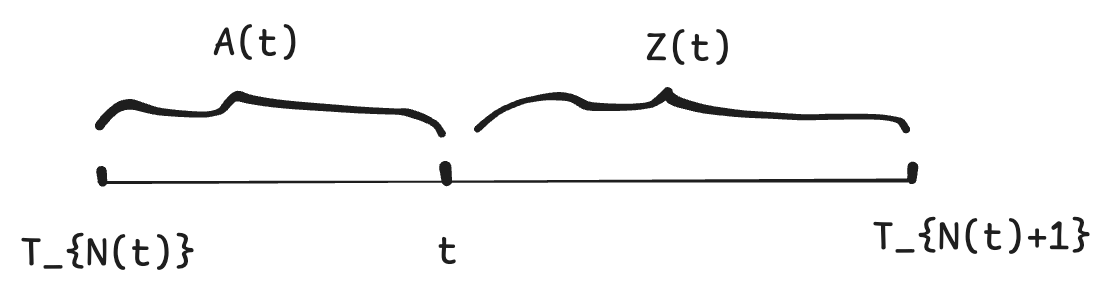
\includegraphics[width=0.55\textwidth]{figures/p119.png}
\end{figure}

$A(t)$ 为使用年龄, $A(t)=t-T_{N(t)}$. $Z(t)$ 为剩余寿命, $Z(t)=T_{N(t)+1}-t$.

\begin{example}
    某零件按更新过程 $\{N(t),t\geq 0\}$ 替换, 其更新间隔时间序列 $\{\tau_k,k\geq 1\}$. 设 $\EE \tau_1^2<\infty$, 且 $0<\EE\tau_1<\infty$, 则零件的长程平均使用年龄
    \[
    \limit{t}\frac{1}{t}\int_0^tA(s)ds=\frac{\EE\tau_1^2}{2\EE\tau_1}
    \]
    若是长程平均寿命即把 $A(s)$ 换成 $Z(s)$.
\end{example}
注: $\int_0^tA(s)ds$有无意义? 有的, 因为 $N(t)$ 是几乎处处右连左极, 在 $[0,t]$ 内有有限多跳. 并非闭区间内的连续函数才可积 (参考梅加强\cite{jiaqiang}).
\begin{figure}[H]
\centering
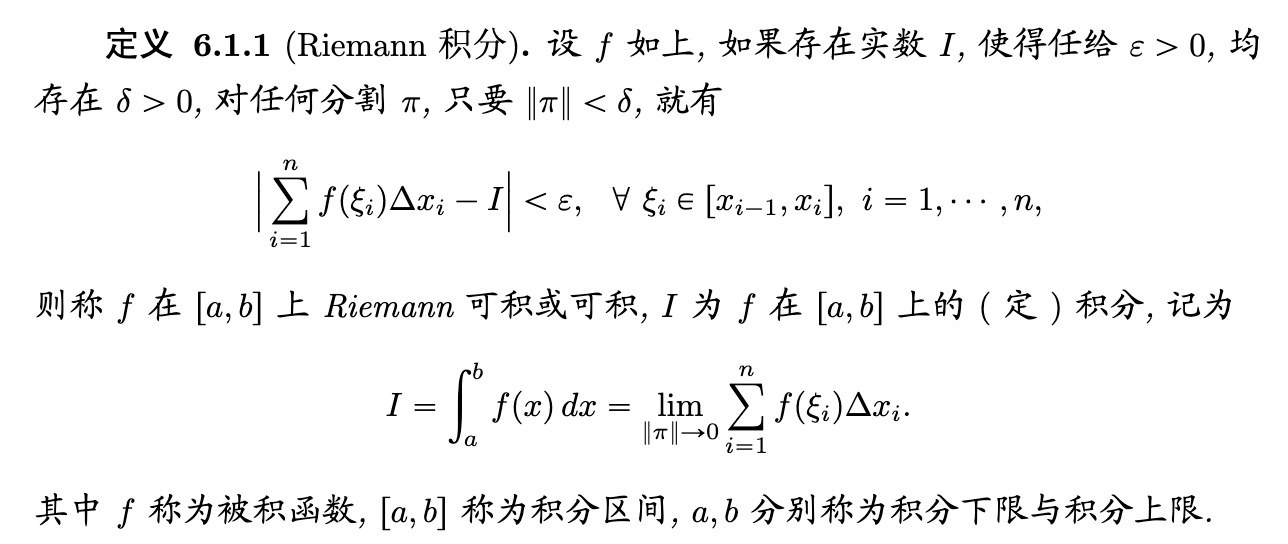
\includegraphics[width=0.75\textwidth]{figures/Riemann-integral.png}
\caption{定义6.1.1-Riemann积分}
\end{figure}

\begin{proof}
    由 $T_{N(t)}\leq t$,
    \[
    \begin{aligned}
        \int_0^t A(s)ds &\geq \int_0^{T_{N(t)}}A(s)ds\\
        &=\sum_{k=1}^{N(t)}\int_{T_{k-1}}^{T_k}(s-T_{N(s)})ds\\
        &=\sum_{k=1}^{N(t)}\int_{T_{k-1}}^{T_k}(s-T_{k-1})ds\\
        &=\sum_{k=1}^{N(t)}\frac{1}{2}(s-T_{k-1})^2\bigg|_{T_{k-1}}^{T_k}\\
        &=\sum_{k=1}^{N(t)}\frac{1}{2}(T_k-T_{k-1})^2=\frac{1}{2}\sum_{k=1}^{N(t)}\tau_k^2
    \end{aligned}
    \]
    由 Thm \ref{thm:p116-thm3.3} 知,
    \[
    \frac{1}{2t}\sum_{k=1}^{N(t)}\tau_k^2\as{t}\frac{\EE \tau_1^2}{2\EE\tau_1}
    \]
    同理,
    \[
    \begin{aligned}
        \int_0^t A(s)ds &\leq \int_0^{T_{N(t)+1}} A(s)ds\\
        &=\sum_{k=1}^{N(t)+1}\frac{1}{2}(T_k-T_{k-1})^2\\
        &=\frac{1}{2}\sum_{k=1}^{N(t)+1}\tau_k^2
    \end{aligned}
    \]
    由 Thm \ref{thm:p116-thm3.3} 知,
    \[
        \frac{1}{2t}\sum_{k=1}^{N(t)}\tau_k^2\as{t}\frac{\EE \tau_1^2}{2\EE\tau_1}
    \]
\end{proof}
\newpage
\pagebreak

\section{连续时间马氏链}
\subsection{定义}

$S$ 至多为可数集 ($S\st \NN$)

\begin{definition}[马氏性]
    称 $S$ 值的过程 $\{X_t,t\geq 0\}$ 具有马氏性, 若对 $\forall n\geq 1,i,j,i_0,\cdots,i_n\in S, 0\leq s_0<s_1<\cdots<s_n<s,t>0$, 有
    \begin{equation}
        \PP(X_{t+s}=j|X_s=i,X_{s_k}=i_k,0\leq k\leq n)=\PP(X_{t+s}=j|X_s=i)
    \end{equation}
    其中, 称 $\PP(X_{t+s}=j|X_s=i)=p_{s,s+t}(i,j)$ 为转移概率.
\end{definition}

\begin{definition}[马氏链]
    称 $\{X_t,t\geq 0\}$ 是一个连续时间马氏链 (CTMC), 若其具有马氏性, 且轨道右连续.
\end{definition}

\begin{definition}[时齐性]
    若 CTMC, $\{X_t,t\geq 0\}$ 的转移概率具有时齐性,
    \[
    p_{s,s+t}(i,j)=p_{0,t}(i,j)\quad \forall i,j\in S, s,t\geq 0
    \]
    称过程是时齐的, 并简记 $p_t(i,j):=p_{s,s+t}(i,j)$.
\end{definition}

\begin{definition}[正则性/标准的]
    称 $\{X_t,t\geq 0\}\sim \CTMC$ 具有正则性, 若
    \[
    \limitto{t}{0^+}p_t(i,j)=\delta_{ij}=\begin{cases}
        1 & i=j\\
        0 & i\neq j
    \end{cases}
    \]
\end{definition}

DTMC的最小步长为1, 因此称一步转移概率矩阵为转移概率矩阵. 但CTMC不存在最小步长, 转移概率矩阵如何给出?

\begin{definition}
    称矩阵族 $\{P_t=(p_t(i,j))_{i,j\in S},t\geq 0\}$ 为过程的 ``转移半群''.
\end{definition}

\begin{theorem}
    $\{P_t,t\geq 0\}$ 为随机半群, 即
    \begin{enumerate}
        \item $\limitto{t}{0^+}P_t=P_0=\II_{S\times S}$ (单位阵)
        \item 对每一个 $P_t$ 都是一个随机矩阵
        \item (C-K方程/半群性质) 对 $\forall s,t\geq 0, P_{s+t}=P_s P_t$, 即
        \[
        p_{s+t}(i,j)=\sum_{k\in S}p_s(i,k)p_t(k,j)
        \]
    \end{enumerate}
\end{theorem}

\begin{proof}
    证明结论 (3).
    \[
    \begin{aligned}
        p_{t+s}(i,j) &=\PP(X_{t+s}=j|X_0=i)\\
        &=\sum_{k\in S}\PP(X_{t+s}=j,X_s=k|X_0=i)\\
        &=\sum_{k\in S}\PP(X_{t+s}=j|X_s=k,X_0=i)\PP(X_s=k|X_0=i)\\
        &=\sum_{k\in S}p_s(i,k)p_t(k,j)
    \end{aligned}
    \]
\end{proof}

\begin{example}
    Poisson过程是时齐CTMC.

    $\PP(N_{t+s}=j|N_s=i)=\PP(N_{t+s}-N_s=j-i|N_s=i)=\PP(N_t=j-i)$
    \[
    p_t(i,j)=\begin{cases}
        e^{-\lambda t}\frac{(\lambda t)^{j-i}}{(j-i)!} & j\geq i\\
        0 & j<i
    \end{cases}
    \]
\end{example}

\begin{example}
    $\{N(t),t\geq 0\}\sim \PoiP(\lambda)\ind \{Y_n,n\geq 1\}\sim \DTMC((u(i,j))_{i,j\in S})$, $\{X_t:=Y_{N(t)},t\geq 0\}\sim\CTMC$
\end{example}

\begin{proof}
    Claim 1: $\displaystyle\PP(X_{t+s}=j|X_s=i)=\sum_{n\geq 0}e^{-\lambda t}\frac{(\lambda t)^n}{n!}\cdot u^{(n)}(i,j)$

    先固定 $N(t)$. $\PP(X_{t+s}=j,X_s=i|N(s)=m,N(t+s)=\tilde{m})=\PP(Y_{\tilde{m}}=j,Y_m=i), 0\leq m\leq \tilde{m}$.
    \[
    \begin{aligned}
        \PP(X_{t+s}=j,X_s=i)&=\sum_{0\leq m\leq \tilde{m}}
        \PP(Y_{\tilde{m}}=j,Y_m=i)\cdot 
        \PP(N(s)=m,N(t+s)=\tilde{m})\\
        &=\sum_{0\leq m\leq \tilde{m}}
        \PP(Y_{\tilde{m}}=j|Y_m=i)\PP(Y_m=i)
        \PP(N(s)=m)\PP(N(t+s)-N(s)=\tilde{m}-m)\\
        &=\sum_{0\leq m\leq \tilde{m}}
        \left[
            u^{(\tilde{m}-m)}(i,j) e^{-\lambda t}\frac{(\lambda t)^{\tilde{m}-m}}{(\tilde{m}-m)!}
        \right]
        \PP(Y_{N(s)}=i,N(s)=m)\\
        &=\sum_{m\geq 0}
        \left(
            \sum_{n\geq 0}u^{(n)}(i,j)e^{-\lambda t}\frac{(\lambda t)^{n}}{n!}
        \right)
        \PP(Y_{N(s)}=i,N(s)=m)\\
        &=\sum_{n\geq 0}u^{(n)}(i,j)e^{-\lambda t}\frac{(\lambda t)^{n}}{n!}\PP(X_s=i)
    \end{aligned}
    \]
    Claim 2: $\forall n\geq 1, i,j,i_0,\cdots,i_n\in S,0\leq s_0<s_1<\cdots<s_n<s,t>0$, 有
    \[
    \PP(X_{t+s}=j|X_s=i,X_{s_k}=i_k,0\leq k\leq n)
    =\sum_{n\geq 0}e^{-\lambda t}\frac{(\lambda t)^n}{n!}u^{(n)}(i,j)
    \]
\end{proof}
\newpage
\subsection{转移速率矩阵与转移概率的计算}
\subsubsection{转移概率的连续性}
\begin{proposition}\label{prop:p122-prop1}
    设 $\{P_t,t\geq 0\}$ 是 $S$ 上的随机半群, 则
    \begin{enumerate}
        \item $\forall t\geq 0,i\in S$, 有 $p_t(i,i)>0$
        \item 若 $\exists s>0$, 使 $p_s(i,i)=1$, 则 $\forall t\geq 0,p_t(i,i)=1$
        \item 若 $\exists s>0$, 使 $p_s(i,j)>0$, 则 $\forall t\geq s,p_t(i,j)>0$
    \end{enumerate}
\end{proposition}

\begin{proof}
\begin{enumerate}
    \item $\limitto{t}{0^+}p_t(i,i)=1\Rightarrow \exists\delta>0,\stt \forall t\in [0,\delta], p_t(i,i)>0$

对 $\forall t\geq 0, \exists s\in [0,\delta),n\in \NN$, 有 $t=s+n\delta$. 故由 C-K 方程, 
\[
\begin{aligned}
    p_t(i,i) &\geq p_{n\delta}(i,i)p_s(i,i)\\
    &\overset{\text{C-K}}{\geq} (p_{\delta}(i,i))^np_s(i,i)>0
\end{aligned}
\]
    \item $p_s(i,i)=1\Rightarrow \forall n\in \NN$, 有 $p_{ns}(i,i)\overset{\text{C-K}}{\geq}(p_s(i,i))^n=1$ ($*1$)
    
    (反证法) 假设 $\exists t>0,\stt p_t(i,i)<1\Rightarrow \sum_{k\neq i}p_t(i,k)>0.  \exists j\neq i,\stt p_t(i,j)>0$ ($*2$).
    
    取 $n$ 使 $ns\geq t$, 则 
    \[
    \begin{aligned}
        p_{ns}(i,i) &=1-\sum_{k\neq i}p_{ns}(i,k)\\
        &\leq 1-p_{ns}(i,j)\\
        &\overset{\text{C-K}}{\leq} 1-p_t(i,j)\underbrace{p_{ns-t}(j,j)}_{>0,\ \text{by}\ (1)}\\
        &< 1\quad \text{by}\ (*2), (1)
    \end{aligned}
    \]
    与 $(*1)$ 矛盾.
    \item $p_s(i,j)>0,p_t(i,j)\geq p_s(i,j)p_{t-s}(j,j)\overset{(1)}{>}0, t\geq s$.
\end{enumerate}
\end{proof}

\begin{theorem}\label{thm:p123-thm1}
    $p_t(i,j)$ 关于 $t\geq 0$ 一致连续, 且对 $t\geq s\geq 0, i,j\in S$.
    \begin{equation}
        |p_t(i,j)-p_s(i,j) |\leq 1-p_{t-s}(i,i)
    \end{equation}
\end{theorem}

\begin{proof}
    \[
    \begin{aligned}
        p_t(i,j)-p_s(i,j) &\xlongequal{\text{C-K}} \sum_{k\in S}p_{t-s}(i,k)p_s(k,j)-p_s(i,j)\\
        &=\sum_{k\neq i}p_{t-s}(i,k) p_s(k,j)-[1-p_{t-s}(i,i)]p_s(i,j)\\
        &=: I_1-I_2
    \end{aligned}
    \]
    $I_1\leq \sum_{k\neq i}p_{t-s}(i,k)=1-p_{t-s}(i,i).\ I_2\leq 1-p_{t-s}(i,i)$. 

    因为 $I_1,I_2$ 非负 $\Rightarrow |\LHS|=|I_1-I_2|=\leq I_1\lor I_2\leq 1-p_{t-s}(i,i)$
\end{proof}

\subsubsection{转移概率的可微性与Kolmogorov方程}

由 Prop \ref{prop:p122-prop1} 和 Thm \ref{thm:p123-thm1} 可证可微性, 但即便如此证明也不是件简单的事, 因此只需要知道下述定理存在即可.

\begin{theorem}\label{thm:p124-thm2}
    $P_t$ 在 $t=0$ 处右导数存在, 具体地,
    \begin{enumerate}
        \item $\forall i\in S$, 下列极限存在.
        \[
        \limitto{t}{0^+}\frac{p_t(i,i)-1}{t}=q(i,i):=-\sup_{t\geq 0}\frac{1-p_t(i,i)}{t}\in [-\infty,0]
        \]
        \item $\forall j\neq i$, 下列极限存在
        \[
            \limitto{t}{0^+}\frac{p_t(i,j)}{t}=q(i,j)\in [0,+\infty)
        \]
        \item $\forall i\in S, \sum_{k\neq i}q(i,k)\leq -q(i,i)$
    \end{enumerate}
\end{theorem}

\begin{definition}[密度矩阵/Q矩阵]
    称 $S$ 上的矩阵 $Q=(q(i,j))_{i,j\in S}$ 为密度矩阵, 若
    \begin{enumerate}
        \item $\forall i\in S,q_i:=-q(i,i)\in [0,+\infty]$
        \item $\forall i,j\in S,q(i,j)\in [0,+\infty)$
        \item $\forall i\in S, \sum_{k\neq i}q(i,k)\leq q_i$
    \end{enumerate}
\end{definition}

\begin{definition}
    由 Thm \ref{thm:p124-thm2} 知, $\{P_t,t\geq 0\}$ 在 $0$ 处的右导数矩阵. $Q:=P_0'=(p_0'(i,j))_{i,j\in S}$ 存在且其为密度矩阵. 称此 $Q$ 为 $\{P_t,t\geq 0\}$ 或 $X$ 的转移速率矩阵/无穷小生成元.
\end{definition}

\begin{definition}
    若 $\forall i,q_i=|q(i,i)|=\sum_{k\neq i}q(i,j)<\infty$ 称密度矩阵 $Q$ 为保守的.
\end{definition}

$\CTMC\to \text{转移半群}\to\text{转移速率矩阵}$. 问: 已知 $Q$, 能否得到 CTMC? 这个问题类比 DTMC 则为: 已知转移矩阵, 能否得到 MC?

\begin{theorem}[Kolmogorov向前/向后方程]
    对具有保守的 $Q$ 的随机半群 $\{P_t,t\geq 0\}$ 有
    \[
    \begin{cases}
        P_t'=QP_t & \text{向后}\\
        P_0=I
    \end{cases}
    \quad
    \begin{cases}
        P_t'=P_t Q & \text{向前}\\
        P_0=I
    \end{cases}
    \]
    注: $AB\neq BA, \text{but}\ QP_t=P_tQ$.
\end{theorem}
\[
\CTMC \overset{+\mu_0}{\iff} \{P_t,t\geq 0\} \overset{P_0'}{\Rightarrow} Q\ (\text{保守的})
\]
反之, 保守的 $Q\Rightarrow \{P_t,t\geq 0\}$

Kolmogorov方程存在唯一性的解, 可以由 $Q$ 构造 CTMC. 侯氏定理.

\begin{theorem}
    在适当的正则性条件下, 有 $Q$ 的向前方程与向后方程存在唯一解, 即 CTMC, $\{P_t,t\geq 0\}+\text{初始分布}\mu_0$, $Q$ 一一对应.
\end{theorem}

\begin{example}[例4.7]
    $\{N(t),t\geq 0\}\sim \PoiP(\lambda)$.
    \[
    p_t(i,j)=\begin{cases}
        e^{-\lambda t}\frac{(\lambda t)^{j-i}}{(j-i)!} & j\geq i\\
        0 & j<i
    \end{cases}
    \]
    \[
    Q=\begin{pmatrix}
        -\lambda & \lambda & 0 & \cdots & \cdots & 0\\
        0 & -\lambda & \lambda & 0 & \cdots & 0\\
        \vdots & \vdots & -\lambda & \lambda & \cdots & 0\\
        \vdots & \vdots & \vdots & \vdots & \cdots & \vdots
    \end{pmatrix}
    \]
    即 $Q(i,i)=-\lambda, Q(i,i+1)=\lambda$.
\end{example}

此前并未限定状态空间有限, 当状态空间有限时:

\begin{corollary}
    设状态空间 $S$ 有限, 则
    \[
    P_t=e^{tQ}=\sum_{n\geq 0}\frac{(tQ)^n}{n!}
    \]
\end{corollary}

\begin{example}[两状态的MC]
    \begin{align*}
        \mathbf{Q}=~
        \bordermatrix{
        &\bf1&\bf2 \cr
        \bf1& -\lambda  & \lambda \cr
        \bf2& \mu & -\mu  \cr
        }~
    \end{align*}
    $\lambda,\mu >0$, 求 $P_t$.
\end{example}

\begin{proof}[解]
    由 Kolmogorov 方程, $P_t'=QP_t$, 即
    \[
    \begin{pmatrix}
        p_t'(1,1) & p_t'(1,2)\\
        p_t'(2,1) & p_t'(2,2)\\
    \end{pmatrix}=
    \begin{pmatrix}
        -\lambda & \lambda\\
        \mu & -\mu
    \end{pmatrix}
    \begin{pmatrix}
        p_t(1,1) & p_t(1,2)\\
        p_t(2,1) & p_t(2,2)
    \end{pmatrix}
    \]
    \[
    \begin{cases}
        p_t'(1,1)=-\lambda p_t(1,1) +\lambda p_t(2,1)\\
        p_t'(2,1)=\mu p_t(1,1)-\mu p_t(2,1)
    \end{cases}
    \]
    \[
    \begin{cases}
        (p_t(1,1)-p_t(2,1))' =-(\lambda+\mu) (p_t(1,1)-p_t(2,1))\\
        p_0(1,1)-p_0(2,1)=1-0=1
    \end{cases}
    \]
    $p_t(1,1)-p_t(2,1)=e^{-(\lambda+\mu)t}$. 代回
    \[
    \begin{cases}
        p_t'(1,1)=-\lambda e^{-(\lambda+\mu)t}\\
        p_0(1,1)=1
    \end{cases},\quad
    \begin{cases}
        p_t'(2,1)=-\mu e^{-(\lambda+\mu)t}\\
        p_0(2,1)=0
    \end{cases}
    \]
    \[
    \begin{aligned}
        p_t(1,1)&=\int_0^t -\lambda e^{-(\lambda +\mu)s}ds+1\\
        &=\frac{\lambda}{\lambda +\mu}e^{-(\lambda+\mu)s}\bigg|_0^t+1=\frac{\lambda}{\lambda+\mu}e^{-(\lambda+\mu)t}+\frac{\mu}{\lambda+\mu}
    \end{aligned}
    \]
    \[
    \begin{aligned}
        p_t(2,1)&=\int_0^t \mu e^{-(\lambda +\mu)s}ds+0\\
        &=\frac{-\mu}{\lambda +\mu}e^{-(\lambda+\mu)s}\bigg|_0^t=\frac{\mu}{\lambda+\mu}-\frac{\mu}{\lambda+\mu}e^{-(\lambda+\mu)t}
    \end{aligned}
    \]
\end{proof}

\subsubsection{轨道的跳跃性质}

探讨 $Q$ 表示了马氏链的什么.

\begin{theorem}\label{thm:p127-thm5}
    设 $S$ 值右连续马氏链 $X:=\{X_t,t\geq 0\}$ 具有保守的转移速率矩阵 $Q=(q(i,j))_{i,j\in S}$. 定义首跳时间 $\eta:=\inf \{t>0|X_t\neq X_0\}$. 其中 $\inf \emp=+\infty$. 那么, 对 $\forall t\geq 0$, 有 $\PP_i(\eta>t)=\PP(\eta>t|X_0=i)=e^{-q_i\cdot t}$, 即在 $\PP_i=\PP(\cdot|X_0=i)$ 下, $\eta\sim \EXP(q_i)$, 其中 $q_i=-q(i,i)$.
\end{theorem}

\begin{corollary}
    若 $q(i,i)=0$, 则 $\PP_i(\eta>t)=1, \forall t\geq 0$. 
\end{corollary}
由 $\{\eta=\infty\}=\cap_{n\geq 1}\{\eta >n\}, \PP_i(\eta=\infty)=1$.
\[
    1=\PP_i(\eta=\infty)=\PP(X_t=X_0,\forall t>0|X_0=i)=\PP(X_t=i,\forall t\geq 0|X_0=i)
\]
即 $i$ 为吸收态.


\begin{proof}[证明 Thm \ref{thm:p127-thm5}]
(Step 1) 
\[
\begin{aligned}
    \limitto{s}{0^+}(p_{st}(i,i))^{1/s} 
    &=\limitto{s}{0^+} \exp\left(
        \frac{\ln p_{st}(i,i)}{st}\cdot t
    \right)\\
    &\xlongequal[x\to 1]{\ln x\sim x-1}\exp\left(
        \limitto{s}{0^+}\frac{p_{st}(i,i)-1}{st}\cdot t
    \right)\\
    &=\exp (t q(i,i))=e^{-q_i t}
\end{aligned}
\]
(Step 2) Claim: $\PP(\eta>t|X_0=i)=\PP(X_s=i,\forall s\in [0,t]|X_0=i)$

``$\Rightarrow$'' $t<\eta =\inf\{t>0|X_t\neq i\}, X_0=i. \forall s\in [0,t],X_s=i$

``$\Leftarrow$'' $X_s=i,\forall s\in [0,t]\Rightarrow X_t=i \xrightarrow{\text{右连续}} \exists \delta>0,\forall u\in [t,t+\delta], \stt X_u=i, \eta\geq t+\delta>t$.

(Step 3) 
\[
\begin{aligned}
    \PP_i(\eta>t)&=\PP_i(X_s=i,\forall s\in [0,t])\\
    &\xlongequal{\text{右连续}}\PP_i(\bigcap_{n\geq 1}\{X_{kt/2^n}=i,k=0,1,\cdots,2^n\}) \quad (*)\\
    &=\limit{n}\PP_i(X_{kt/2^n}=i,k=0,1,\cdots,2^n)\\
    &=\limit{n}(p_{t/2^n}(i,i))^{2^n}=e^{-q_i t}
\end{aligned}
\]
$(*)$ 是一个数分结论, 回去证明. $\forall s$ 可找到一列 $n$ 逼近.
\end{proof}
令 $T_0=0$, 归纳定义 $T_n:=\inf \{t>0|X_t\neq X_{T_{n-1}}\},n\geq 1$. $T_1$ 即上面的 $\eta$.

$T_n$: 第$n$次跳跃时间 $(T_1=\eta)$

\begin{lemma}
    设右连续马氏链$X$具有保守的$Q$, 则
    \begin{enumerate}
        \item 在 $[0,\limit{n}T_n)$ 上, $X$的轨道为阶梯函数, 即 $X_t=X_{T_n},t\in[T_n,T_{n+1}]$.
        \item 若 $q_i>0$, 则 $\{X_{T_n},n\geq 1\}\sim\DTMC(\hat{P})$, 其中
        \[
        (\hat{P})_{ij}=\hat{p}_{ij}=\frac{q(i,j)}{q(i)}(1-\delta_{ij})
        \]
        称 $\{X_{T_n},n\geq 1\}$ 为 $X$ 的嵌入链.
    \end{enumerate}
\end{lemma}

(走神)

\subsubsection{过程的构造}
设 $Q=(q(i,j))_{i,j\in S}$ 为保守的密度矩阵, 其中
\[
q_i=-q(i,i)=\sum_{k\neq i}q(i,k)
\]
假定 $q(i,i)>0, \forall i\in S$, 假设没有吸收态. (实际上无需此假设也成立, 但此处为了和教材一致)

定义 $\hat{P}:=(\hat{p}_{i,j})_{i,j\in S}$, 其 $\hat{p}_{ij}=\frac{q(i,j)}{q(i)}(1-\delta_{ij})$, 则 $\hat{P}$ 为随机矩阵, 并称其路径矩阵.

两种看过程的角度:
\begin{enumerate}
    \item $X(t,\cdot)$ r.v. $\forall t\geq 0$
    \item $X(\cdot,\omega)\in C([0,+\infty))$
\end{enumerate}

设
\begin{enumerate}
    \item $\{Y_n,n\geq 0\}\sim \DTMC(\mu_0,\hat{P})$
    \item $\tau_0,\tau_1,\cdots \overset{\text{iid}}{\sim} \EXP(1)$, 注: $\tau_n/q_i\sim \EXP(q_i)$
    \item $\{\tau_k,k\geq 0\}\ind \{Y_n,n\geq 0\}$
\end{enumerate}
下面构造 CTMC.
\begin{enumerate}
    \item $t=n$ 时, 处于状态 $Y_0$, $\eta_1=\tau_0/q(Y_0)\sim \EXP(q(i))$ 在 $\PP(\cdot|Y_0=i)$, 记 $\eta_1\sim \EXP(Y_0)$.
    \item $t=T_1=\eta_1$ 时, 跳到状态 $Y_1$, 在 $Y_1$ 待了 $\eta_2=\tau_1/q(Y_1)\sim\EXP(Y_1)$
    \item $t=T_2=\eta_1+\eta_2$ 时, 跳到状态 $Y_2$, 在 $Y_2$ 待了 $\eta_3=\tau_2/q(Y_2)\sim\EXP(Y_2)$
\end{enumerate}
由此类推, $\eta_n=\tau_{n-1}/q(Y_{n-1}),\forall n\geq 1. T_n=\sum_{k=1}^n\eta_k,T_0=0$.

令 $X_t=Y_n$ (当 $t\in [T_n,T_{n+1}]$), 若
\begin{equation}
    \PP(\limit{n}T_n=+\infty|X_0=Y_0=i)=1
    \label{eq:p129-**}
\end{equation}
称 $X$ 为以 $Q$ 为速率矩阵的跳过程, 称 $Y$ 为 $X$ 的嵌入链, $\{\eta_k,k\geq 1\}$ 为 $X$ 的等待时间序列, $T_n$ 为第 $n$ 次跳的时刻.

注: $\forall t\geq 0$, 至多有限个 $n, \stt T_n\leq t$.

\begin{lemma}
    以 $Q$ 为速率矩阵的跳过程 $X$ 是一个 CTMC, 且 $X\sim \CTMC(Q)$ 以及 $P_t'=QP_t,P_t'=P_t Q$. 其中 $\{P_t,t\geq 0\}$ 是 $X$ 的转移半群.
\end{lemma}

注: $X\sim \CTMC(\mu_0,(P_t)_{t\geq 0})$ (有限维分布族)

$\Rightarrow X\sim \CTMC(\mu_0,Q)$

$\Leftarrow$ Kolmogorov方程的适定性

$\tilde{X}\sim \text{跳过程}(\mu_0,Q)\sim \CTMC (\mu_0,(\tilde{P}_t)_{t\geq 0})$

且 Kolmogorov 方程 $\tilde{P}_t'=\tilde{P}_t Q=Q \tilde{P}_t, \Rightarrow P_t=\tilde{P}_t$, 即 $X\overset{(d)}{=}\tilde{X}$.

\eqref{eq:p129-**} 不好验证, 有什么好验证的充分条件使其成立吗?

\begin{lemma}
    若 $\{q_i,i\in S\}$ 有界, 则条件 \eqref{eq:p129-**} 成立. 特别地, $S$ 有限, 则条件 \eqref{eq:p129-**} 成立.
\end{lemma}

\begin{example}[纯生过程]
    $S=\{1,2,3,\cdots\}, \lambda_1,\lambda_2,\cdots$ 为一列正数. 令 $q_i=q(i,i+1)=\lambda_i,\forall i\geq 1$, 称出生速率.
    \[
    Q=\begin{pmatrix}
        -\lambda_1 & \lambda_1 & 0 & \cdots &\cdots & \cdots\\
        0 & -\lambda_2 & \lambda_2 & 0 &\cdots & \cdots\\
        0 & 0 & -\lambda_3 & \lambda_3 & 0 &\cdots \\
        \vdots & \vdots & & \ddots & \ddots & 
    \end{pmatrix}
    \]
\end{example}

转移速率图:
\[
1\xrightarrow{\lambda_1} 2\xrightarrow{\lambda_2} 3 \xrightarrow{\lambda_3} 4\cdots
\]
Claim: \eqref{eq:p129-**} 成立 $\iff \sum_{n=1}^{\infty}1/\lambda_n=\infty$.
\begin{enumerate}
    \item Poisson过程 $\PoiP(\lambda)$ 为纯生过程
    \item (Durrett Exa 4.5) $q_i=q(i,i+1)=\lambda i^p,\forall i\geq 1$
    \[
    \sum_{n=1}^{\infty}\frac{1}{\lambda_n}
    =\frac{1}{\lambda}\sum_{n=1}^{\infty}\frac{1}{n^p}
    =\begin{cases}
        <\infty & p>1\\
        \infty & p\leq 1
    \end{cases}
    \]
    $p\in [0,1]$ 时, 可定义由 $Q$ 为速率矩阵的跳过程. $p=0$ 时为 Poisson 过程. 特别地, $p=1$ 时称为 Yule 过程.
    \item $\sum_{n=1}^{\infty}1/\lambda_n=\infty$ 时, 嵌入链 $\{Y_n,n\geq 0\}\sim \DTMC(\hat{P})$, 其中
    \[
    (\hat{P})_{i,j}=\hat{p}_{i,j}=\frac{q(i,j)}{q(i)}(1-\delta_{ij})\Rightarrow \hat{p}_{i,i+1}=1
    \]
\end{enumerate}

\begin{example}[生灭过程]
    $S=\{0,1,2,3,\cdots\}$ 令 $q(i,i+1)=\lambda_i,\forall i\geq 0$ (出生速率). $q(i,i-1)=\alpha_i,\forall i\geq 1$ (死亡速率), 其他为0.
    \[
    q_i=-q(i,i)=\sum_{k\neq i}q(i,k)=\begin{cases}
        \lambda_i+\alpha_i & i\geq 1\\
        \lambda_i & i=0
    \end{cases}
    \]
\end{example}
转移速率图:
\[
0
\xleftrightharpoons[\lambda_0]{\alpha_1} 1
\xleftrightharpoons[\lambda_1]{\alpha_2} 2
\xleftrightharpoons[\lambda_2]{\alpha_3} 3
\]
Claim: 若 $\exists c>0$, 使 $\lambda_i\lor \alpha_i\leq c_i(\forall i\geq 1)$, 则 \eqref{eq:p129-**} 成立. 故而此时可定义 $Q=(q(i,j))_{i,j\in S}$ 对应的跳过程, 称其为生灭过程. (证明不是件容易的事, 因此只记结论)

嵌入链 $\{Y_n,n\geq 0\}\sim\DTMC(\hat{P})$, 其中
\[
(\hat{P})_{i,j\in S}=: \hat{p}_{ij}=\frac{q(i,j)}{q(i)}(1-\delta_{ij})=
\begin{cases}
    \lambda_0/\lambda_0=1 & i=0,j=1\\
    \frac{\lambda_i}{\lambda_i+\alpha_i} & j=i+1,i\geq 1\\
    \frac{\alpha_i}{\lambda_i+\alpha_i} & j=i-1,i\geq 1\\
    0 & \text{otherwise}
\end{cases}
\]
转移概率图
\[
0
\xleftrightharpoons[1]{\alpha_1/(\lambda_1+\alpha_1)} 1
\xleftrightharpoons[\lambda_1/(\lambda_1+\alpha_1)]{\alpha_2/(\lambda_2+\alpha_2)} 2
\xleftrightharpoons[\lambda_2/(\lambda_2+\alpha_2)]{\alpha_3/(\lambda_3+\alpha_3)} 3
\xleftrightharpoons[]{}\cdots
\]
$\{Y_n,n\geq 1\}$ 是生灭链.

\begin{example}[排队系统]
    描述 $t$ 时刻系统里的顾客数/队列长度 (=在等待的顾客数+正在被服务的顾客)
    \begin{enumerate}
        \item 要素
        \begin{itemize}
            \item 到达过程/到达速率
            \item 服务时长/服务速率 (指数分布时)
            \item 服务台数/窗口/服务员
        \end{itemize}
        \item 队列容量
        \item 服务规则
        \begin{enumerate}
            \item 先到先得 (FCFS)
            \item 服务时长相互独立
        \end{enumerate}
        \item M/M/S
        \begin{enumerate}
            \item M: Markovian/Memoryless, 到达过程$\sim \PoiP(\lambda)$
            \item M: Memoryless, 服务时长 $\sim\EXP(\alpha)$
            \item S: 服务台数 $\in [1,+\infty)\cap \NN$
        \end{enumerate}
    \end{enumerate}
\end{example}

\begin{enumerate}
    \item M/M/1. 
    
    $S=\{0,1,2,\cdots\}, q(n,n+1)=\lambda (\forall n\geq 0), q(n,n-1)=\alpha (\forall n\geq 1)$

    由前例知, M/M/1 排队系统是生灭过程.
    \begin{enumerate}
        \item $q(i)$
        \[
        q(i)=-q(i,i)=\begin{cases}
            \lambda & i=0\\
            \sum_{k\neq i}q(i,k)=\lambda +\alpha & \forall i\geq 1
        \end{cases}
        \]
        \item 嵌入链 $\{Y_n,n\geq 1\}\sim \DTMC(\hat{P})$, 其中 $\displaystyle (\hat{P})_{i,j}=:\hat{p}_{ij}=\frac{q(i,j)}{q(i)}(1-\delta_{ij})$. 
    \end{enumerate}
    $\displaystyle \Rightarrow \hat{p}_{0,1}=\frac{\lambda}{\lambda}=1,\hat{p}_{i,i+1}=\frac{\lambda}{\lambda+\alpha}(\forall i\geq 1), \hat{p}_{i,i-1}=\frac{\alpha}{\lambda+\alpha}(\forall i\geq 1)$.

    记 $p=\frac{\lambda}{\lambda+\alpha},1-p=\frac{\alpha}{\lambda+\alpha}$, 看出 $\{Y_n,n\geq 1\}$ 是带反射壁的随机游动.
    \item M/M/S
    
    $S=\{0,1,2,\cdots\}, q(n,n+1)=\lambda (\forall n\geq 0)$
    \[
    q(n,n-1)=\begin{cases}
        s\alpha & n\geq s\\
        n\alpha & n\leq s
    \end{cases}
    \]
    由前例知, M/M/S 也是生灭过程
    \item M/M/$\infty$
    
    $S=\{0,1,2,\cdots\}, q(n,n+1)=\lambda (\forall n\geq 0), q(n,n-1)=n\alpha (\forall n\geq 1)$

    由前例知, M/M/$\infty$ 也是生灭过程
\end{enumerate}
\newpage
\subsection{平稳分布与极限行为}

\subsubsection{平稳分布}

$d(i):=\gcd\{n\geq 1|p_{ii}(n)>0\}$. (正则) CTMC $\Rightarrow t\geq 0,i\in S,p_t(i,i)>0\Rightarrow$ 非周期

\begin{definition}[不可约]
    称 CTMC 不可约, 若 $\forall i,j\in S$, 存在一个状态序列 $k_0=i,k_1,\cdots,k_n=j$, 使 $q(k_{m-1},k_m)>0(1\leq m\leq n)$.
\end{definition}

\begin{lemma}\label{lem:p133-lem1}
    $q(i,j)>0,\forall i\neq j\Rightarrow p_t(i,j)>0,\forall t>0$.
\end{lemma}

\begin{proof}
    \[
    0<q(i,j)=\limitto{h}{0^+}\frac{p_h(i,j)}{h}
    \]
    $\exists \delta>0,\forall s\in (0,\delta],\stt p_s(i,j)>0$. 

    由 Prop \ref{prop:p122-prop1} 知, $p_t(i,j)>0,\forall t>0,i\neq j$.
\end{proof}

\begin{lemma}
    若 $X$ 不可约, 则 $p_t(i,j)>0 (\forall t>0,i,j\in S)$
\end{lemma}

\begin{proof}
    $X$ 不可约 $\Rightarrow$ 对 $i\neq j$, 存在一个状态序列 $k_0=i,k_1,\cdots,k_n=j$, 使 $q(k_{m-1},k_m)>0(1\leq m\leq n)\xrightarrow{\text{Lem}\ \ref{lem:p133-lem1}} p_t(k_{m-1},k_m)>0, (1\leq m\leq n)$
    \[
    p_t(i,j)\overset{\text{C-K}}{\geq } p_{t/n}(k_0,k_1)p_{t/n}(k_1,k_2)\cdots p_{t/n}(k_{n-1},k_n)>0,\forall t>0
    \]
\end{proof}

回忆平稳分布
\begin{itemize}
    \item DTMC: $\pi P=\pi\iff \pi P^n=\pi(\forall n\geq 1)$
    \item CTMC: 没有最小步长 (实数轴不稀疏)
\end{itemize}
因此 CTMC 的平稳分布是这样定义的:

\begin{definition}[平稳分布]
    称概率分布 $\pi$ 为本群 $\{P_t,t\geq 0\}$ 的平稳分布, 若 $\pi P_t=\pi(\forall t\geq 0)$ 
\end{definition}

然而, 这个条件难以验证. 除了转移半群, 还可以用转移速率 $Q$ 刻画.
\[
Q=\begin{cases}
    q(i,j) & i\neq j\\
    q(i,i)=-q(i) & i=j
\end{cases}
\]
其中, $q(i)=\sum_{k\neq i}q(i,k)$ 状态 $i$ 的总转移速率

\begin{lemma}\label{lem:p134-lem4.3}
    $\pi$ 是平稳分布 $\iff \pi Q=0$, 故而 $\pi$ 是 $Q$ 的平稳分布.
\end{lemma}

\begin{proof}
    ``$\Rightarrow$'' $\pi P_t=\pi(\forall t\geq 0)\Rightarrow \frac{d}{dt}(\pi P_t)=0\Rightarrow \pi P_t'=0$. 又 $P_t'=P_t Q$, 故 $\pi P_t Q=0\Rightarrow \pi Q=0$

    ``$\Leftarrow$'' $\pi Q=0\Rightarrow (\pi P_t)'=\pi P_t'=\pi (QP_t)=0$

    $\pi P_t=\pi P_0=\pi$
\end{proof}

\subsubsection{极限行为}

回顾 (DTMC): 不可约, 非周期, 则存在平稳分布$\pi$
\[
\limit{n}P^(n)(i,j)=\pi(j)\quad \forall i,j\in S
\]
\begin{theorem}[Convergence to Equilibrium]
    设 $\{X_t,t\geq 0\}$ 为 CTMC, 转移速率矩阵 $Q$, 不可约. 存在平稳分布 $\pi\Rightarrow \limit{t}p_t(i,j)=\pi(j), \forall i,j\in S$.

    注: 存在 $\pi$ 则唯一 (极限的唯一性)
\end{theorem}

\begin{proof}
    (Step 1) $Q$ 不可约 $\xrightarrow{\text{Lem}\ \ref{lem:p134-lem4.3}} \boxed{p_t(i,j)>0}(\forall t>0,i,j\in S)$. 固定 $h>0$ (步长), 考虑 h-骨架 $\{Z_n:=X_{nh},n\geq 0\}$. 根据定义验证 $Z\sim\DTMC(P_h)$ 且不可约 (方框), 非周期, $\pi$ 也是 $Z$ 的平稳分布.

    $\Rightarrow \limit{n}p_{nh}(i,j)=\pi(j)$. (海涅原理?)

    (Step 2) 
    \[
    \begin{aligned}
        |p_t(i,j)-\pi(j)|&\leq |p_t(i,j)-p_{nh}(i,j)|+|p_{nh}(i,j)-\pi(j)|\\
        &\leq 1-p_{|t-nh|}(i,i)+|p_{nh}(i,j)-\pi(j)|
    \end{aligned}
    \]
    $\forall \epsilon>0,\exists h>0,\stt\forall s\in [0,h], 1-p_s(i,i)<\epsilon/2$

    对同一个 $h, \exists N>0,\stt \forall n>N, |p_{nh}(i,j)-\pi(j)|<\epsilon/2$

    $\forall t\geq Nh, \exists n\geq N, \stt nh\leq t<(n+1)h$, 则 $|t-nh|<h$
    \[
    |p_t(i,j)-\pi(j)|\leq 1-p_{|t-nh|}(i,i)+|p_{nh}(i,j)-\pi(j)|<\epsilon/2+\epsilon/2=\epsilon
    \]
    $\limit{t}p_t(i,j)=\pi(j)$.
\end{proof}

\subsubsection{细致平衡条件(DBC)}

\begin{definition}
    $\pi$为概率分布, 若 $\forall j\neq k$ 有 $\pi(j)q(j,k)=\pi(k)q(k,j)$, 则称 $\pi$ 与 $Q$ 满足DBC.
\end{definition}

\begin{theorem}
    若 $\pi$ 与 $Q$ 满足 DBC $\Rightarrow \pi$ 平稳分布

    注: 反例 4.10
\end{theorem}

\begin{proof}
    DBC $\Rightarrow \pi(k)q(k,j)=\pi(j)q(j,k),\forall k,j\in S$. 关于 $k$ 求和
    \[
    \begin{aligned}
        \sum_{k\in S}\pi(k)q(k,j) &=\pi(j)\sum_{k\in S}q(j,k)\\
        &=\pi(j)\sum_{k\neq j}q(j,k)+\pi(j)q(j,j)\\
        &=0
    \end{aligned}
    \]
    $\therefore \pi Q=0$.
\end{proof}

\begin{example}[生灭链]\label{exa:p136-exa4.12}
    $S=\{0,1,2,\cdots,N\}$或$\{0,1,2,\cdots\}. q(n,n+1)=\lambda_n(\forall n\geq 0), q(n,n-1)=\alpha_n (\forall n\geq 1)$. 设所有 $\lambda_n,\alpha_n>0$ (即不考虑纯生过程), 故不可约. 求满足 DBC 的平稳分布 $\pi$.
\end{example}

\begin{proof}[解]
    DBC $\Rightarrow \pi(n-1)q(n-1,n)=\pi(n)q(n,n-1), \forall n\geq 1$.
    \[
    \pi(n)=\frac{\lambda_{n-1}}{\alpha_n}\pi(n-1)=\frac{\prod_{k=0}^{n-1}\lambda_k}{\prod_{k=1}^n\alpha_k}\pi(0)=:c_n \pi(0), c_0=1
    \]
    \[
    1=\sum_{n=0}^N \pi(n)=\sum_{n=0}^N c_n\pi(0)\iff \pi(0)=\frac{1}{\sum_{n=0}^N c_n}>0
    \]
    记 $c:=\sum_{n=0}^N c_n<\infty$. $\pi(n)=c_n/c(\forall n\geq 0)$ 满足DBC的平稳分布.
\end{proof}

\begin{example}[M/M/$\infty$ 排队系统]
    $S=\{0,1,2,\cdots\},q(n,n+1)=\lambda(\forall n\geq 0), q(n,n-1)=n\alpha(n\geq 1)$.    
\end{example}

令 $c_0=1$,
\[
c_n=\frac{\prod_{k=0}^{n-1}\lambda}{\prod_{k=1}^n(k\alpha)}=\frac{\lambda^n}{n!\alpha^n}(\forall n\geq 1)
\]
\[
c=\sum_{n=1}^{\infty}c_n=\sum_{n=0}^{\infty}\frac{\lambda^n}{n!\alpha^n}=e^{\lambda/\alpha}<\infty
\]
$\pi=(c_0/c, c_1/c, \cdots)$ 为 M/M/$\infty$ 的平稳分布且满足 DBC. $\pi(n)=c_n/c=\frac{\lambda^n}{n!\alpha^n}e^{-\lambda/\alpha}$ 即 $\pi\sim \Poi(\lambda/\alpha)$.

\begin{example}[有止步的M/M/S排队系统]
    $S$个服务员,服务时长$\sim \EXP(\alpha)$. 顾客到达过程 $\sim\PoiP(\lambda)$. $q(n,n+1)=\lambda a_n(\forall n\geq 0)$, 
    \[
    q(n,n-1)=\begin{cases}
        n\alpha & 0\leq n\leq s\\
        s\alpha & n\geq s
    \end{cases}
    \]
\end{example}

\begin{theorem}
    若 $\limit{n}a_n=0$, 则存在一平稳分布
\end{theorem}

\begin{proof}
    令 $c_0:=1, c_n=\prod_{k=0}^{n-1}(\lambda_k)/\prod_{k=0}^n(\alpha_k), \forall n\geq 1$. 若 $c:=\sum_{n=0}^{\infty}c_n<\infty$, 则由例 \ref{exa:p136-exa4.12}, 存在平稳分布 $\pi=(c_0/c,c_1/c,\cdots)$

    下证: $\limit{n}a_n=0\Rightarrow c<\infty$.

    对 $n>s$,
    \[
    c_n=\frac{\prod_{k=0}^{n-1}(\lambda a_k)}{(\prod_{k=0}^s k\alpha)(\prod_{k=s+1}^n s\alpha)}=\prod_{k=0}^{n-1}(\frac{\lambda a_k}{s\alpha})\cdot \frac{\prod_{k=1}^s(s\alpha)}{\prod_{k=1}^s (k\alpha)}=:\prod_{k=0}^{n-1}(\frac{\lambda a_k}{s\alpha})\cdot A
    \]
    $\limit{n}a_n=0 \Rightarrow $ 取 $\epsilon=1/2$, 则 $\exists N>0,\forall n>N,\stt \frac{\lambda a_n}{s\alpha}<1/2$. 对 $\forall n>N\lor s$, 有 $0\leq c_n\leq A\cdot (\frac{1}{2})^n$. $c=\sum_{n=0}^{\infty}c_n<\infty$.
\end{proof}

\subsubsection{访问频率/渐进频率}

回顾 DTMC. 设$X$不可约, $\pi$是平稳分布, 则
\[
\limit{n}\frac{N_n(y)}{n}=\pi(y)=\frac{1}{\EE_y T_y}
\]
其中 $T_y:=\min\{n\geq 1|X_n=y\}, N_n(y)=\sum_{k=0}^n\II_{\{X_k=y\}}$.

对于 CTMC, $\sigma_i:=\inf\{t>\eta|X_t=i\}$, 其中 $\eta:=\inf\{t\geq 0|X_t\neq X_0\}$ 为首次跳跃时刻.

\begin{theorem}[访问频率]
    $X$不可约, $\pi$是平稳分布, 则
    \[
    \limit{t}\frac{\int_0^t \II_{\{X_i=s\}}ds}{t}=\limit{t}\frac{\EE \int_0^t \II_{\{X_i=s\}}ds}{t}=\pi(i)=\frac{1}{\EE_i \sigma_i q_i}
    \]
    注: CTMC下的测度是用积分定义的, $\int_0^t\II_{\{X_i=s\}}ds$ 为 $[0,t]$ 内落到状态$i$的时长.
\end{theorem}

\begin{example}[理发店: 有止步的M/M/1系统]
    $S=\{0,1,2,3\}$, 到达过程 $\sim \PoiP(\lambda),\lambda=2$, 服务时长 $\sim\EXP(\alpha),\alpha=3\text{个/h}$. 均值 $\frac{1}{3}h=20$min. $q(n,n+1)=\lambda(0\leq n\leq 2), q(n,n-1)=\alpha(1\leq n\leq 3)$.
    \begin{enumerate}
        \item[(a)] 求均衡分布.
        \item[(b)] 未接受服务的顾客.
    \end{enumerate}
\end{example}

\begin{proof}[解]
    \begin{enumerate}
        \item[(a)] $S$不可约, 故若存在平稳分布, 则唯一. 由例\ref{exa:p136-exa4.12}知, 有平稳分布 $\pi=(c_0/c,\cdots,c_3/c)$. 其中 $c_0=1,c_n=\prod_{k=0}^{n-1}\lambda/\prod_{k=1}^{n}\alpha=(\frac{\lambda}{\alpha})^n=(\frac{2}{3})^n, 1\leq n\leq 3$.
        \[
        c=1+\frac{2}{3}+(\frac{2}{3})^2+(\frac{2}{3})^3=\frac{1\cdot (1-(2/3)^4)}{1-2/3}=\frac{65}{27}
        \]
        \item[(b)] 
        \[
        \limitto{t}{0}\frac{\int_0^t \II_{\{X_s=3\}}ds}{t}=\pi(3)=(\frac{2}{3})^3/\frac{65}{27}=\frac{8}{65}
        \]
    \end{enumerate}
\end{proof}
\newpage

\pagebreak

\section{离散鞅}
\subsection{定义}

\begin{definition}[流]
    称一列$\sigma$代数 $\CF_1,\CF_2,\cdots$ 为$\Omega$上的流, 若 $\CF_1\st \CF_2\st \CF_3\st\cdots$
\end{definition}

\begin{definition}[适应过程]
    称一列随机变量 $(X_n)_{n\geq 0}$ 关于流 $(\CF_n)_{n\geq 0}$ 适应的, 若 $\sigma(X_n)\st \CF_n$, 即 $X_n\in \CF_n$, $X_n$关于$\CF_n$可测.
\end{definition}
注: 离散 $\Rightarrow$ 默认 $\sigma$-代数由划分生成, 一系列性质在 Chap 1 中被严格证明.

\begin{example}[自然流]
    设$(X_n)_{n\geq 0}$ 为一列随机变量列, 对$\forall n\geq 0$, 由 Def \ref{def:multi_rv_con_exp}, 令 $\CF_n^X=\sigma(X_0,\cdots,X_n)=(X_0,\cdots,X_n)^{-1}(2^{S_0}\times\cdots\times 2^{S_n})$, 则 $(\CF_n^X)_{n\geq 0}$ 为一个流, 称为 $(X_n)_{n\geq 0}$ 的自然流.
\end{example}

\begin{definition}[离散鞅]\label{def:p140-def3}
    称随机变量列 $(X_n)_{n\geq 0}$ 关于流 $(\CF_n)_{n\geq 0}$ 的鞅, 若
    \begin{enumerate}
        \item (可积性) $\forall n\geq 0, \EE|X_n|<\infty$
        \item (适应性) $(X_n)_{n\geq 0}$ 关于 $(\CF_n)_{n\geq 0}$ 适应
        \item (鞅性) $\forall n\geq 0, \EE(X_{n+1}|\CF_n)\xlongequal{\text{a.s.}}X_n$
    \end{enumerate}
\end{definition}

\begin{theorem}
    \begin{enumerate}
        \item (Durrett, Thm 5.1) 设 $(X_n)_{n\geq 0}$ 关于 $(\CF_n)_{n\geq 0}$ 的鞅, 则 $\EE X_n=\EE X_0$.
        \item 设 $(X_n)_{n\geq 0}$ 为关于 $(\CF_n)_{n\geq 0}$ 适应的可积随机变量列, 则 
        
        $(X_n)_{n\geq 0}$ 为关于 $(\CF_n)_{n\geq 0}$ 的鞅 $\iff$ $\EE(X_{n+1}-X_n|\CF_n)=0,\forall n\geq 0$.
    \end{enumerate}
\end{theorem}

\begin{proof}
    \begin{enumerate}
        \item $\EE X_{n+1}=\EE(\EE(X_{n+1}|\CF_n))\xlongequal{\text{鞅性}}\EE(X_n)\xlongequal{\text{迭代}}\EE X_0$
        \item ``$\Rightarrow$'' $\EE(X_{n+1}-X_n|\CF_n)=X_n-\EE(X_n|\CF_n)\xlongequal{X_n\in \CF_n}X_n-X_n=0$. (提取已知量)
        
        ``$\Leftarrow$'' $\EE(X_{n+1}|\CF_n)=\EE(X_{n+1}-X_n|\CF_n)+\EE(X_n|\CF_n)=X_n$
    \end{enumerate}
\end{proof}

\begin{example}
    常数列 $\{c_n=c,n\geq 0\}$ 关于任意流都是鞅. $c=c\II_{\Omega}, \sigma(c)=\{\emp,\Omega\}\st \CF_n$
\end{example}

\begin{definition}
    称 $(X_n)_{n\geq 0}$ 是关于 $(Y_n)_{n\geq 0}$ 的鞅. 若 $(X_n)_{n\geq 0}$ 关于 $Y$ 的自然域流 $\CF_n^Y=\sigma(Y_0,\cdots,Y_n),n\geq 0$ 是鞅.
\end{definition}

\begin{definition}
    若 Def \ref{def:p140-def3} 中 (3) 为 ``$\leq$'' 时, 即 $\EE(X_{n+1}|\CF_n)\leq X_n$, 称为上鞅. 若为``$\geq$'' 时, 即 $\EE(X_{n+1}|\CF_n)\geq X_n$, 称为下鞅.
\end{definition}

\begin{definition}
    \begin{enumerate}
        \item $X$ 鞅 $\iff$ $X$ 上鞅, 下鞅
        \item $X$ 上鞅 $\iff$ $-X$ 下鞅
    \end{enumerate}
\end{definition}

\begin{theorem}[Durrett, Thm 5.9\& 5.10]
    \begin{enumerate}
        \item 设 $(M_n)_{n\geq 0}$ 关于 $(\CF_n)_{n\geq 0}$ 是一个上鞅, 则 $\EE M_{n+1}\leq \EE M_n$ (期望 $\downarrow$)
        \item 设 $(M_n)_{n\geq 0}$ 关于 $(\mc{S}_n)_{n\geq 0}$ 是一个下鞅, 则 $\EE M_{n+1}\geq \EE M_n$ (期望 $\uparrow$)
    \end{enumerate}
\end{theorem}

\begin{proof}
    (1) $\EE M_{n+1}=\EE(\EE(M_{n+1}|\CF_n))\leq \EE(M_n)$. (2) 同理.
\end{proof}

\begin{theorem}
    设 $(X_n)_{n\geq 0}$ 关于 $(\CF_n)_{n\geq 0}, (\mc{S}_n)_{n\geq 0}$ 均适应的, 且关于 $(\CF_n)_{n\geq 0}$ 是鞅, $\mc{S}_n\st \CF_n (\forall n\geq 0)$, 则
    \begin{enumerate}
        \item $(X_n)_{n\geq 0}$ 关于 $(\mc{S}_n)_{n\geq 0}$ 也是鞅 (小流吃大流)
        \item 特别地, $(X_n)_{n\geq 0}$ 关于其自然域流 $\CF_n^X:=\sigma(X_0,\cdots,X_n), n\geq 0$ 是鞅 
    \end{enumerate}
\end{theorem}

注: $\Pi_1,\Pi_2$ 是 $\Omega$ 上的两个划分, $\Pi_1\st \Pi_2$, 故 $\sigma(\Pi_1)\st \sigma(\Pi_2)$, 则
\[
\EE\bigg(
    \EE(
        \underbrace{X|\sigma(\Pi_1)}_{\in \sigma(\Pi_1)\st \sigma(\Pi_2)}
    )\bigg| \sigma(\Pi_2)
\bigg)=\EE(X|\sigma(\Pi_1))
\]
\[
\EE\bigg(
    \EE(
        X|\sigma(\Pi_1)
    )\bigg| \sigma(\Pi_2)
\bigg)=
\EE\bigg(
    \EE(
        X|\sigma(\Pi_2)
    )\bigg| \sigma(\Pi_1)
\bigg)
\]
\begin{proof}
    (1) (可积性) $X$关于$\CF_n$是鞅 $\Rightarrow$ $\EE|X|<\infty$

    (适应性) $X$ 关于 $\mc{S}$ 适应

    (鞅性) $\EE(X_{n+1}|\mc{S}_n)=\EE(\EE(X_{n+1}|\mc{S}_n|\mc{F}_n)=\EE(\EE(X_{n+1}|\CF_n)|\mc{S}_n)=\EE(X_n|\mc{S}_n)=X_n$
\end{proof}
\subsection{基本性质与例子}

\begin{property}[Durrett, Lem 5.7]\label{prt:p142-prt1}
设 $(M_n)_{n\geq 0}$ 关于 $(\CF_n)_{n\geq 0}$ 是一个鞅, 则 $\forall n\geq 0$,
\[
\EE(M_{n+1}^2|\CF_n)-M_n^2=\EE(M_{n+1}^2-M_n^2|\CF_n)=\EE((M_{n+1}-M_n)^2|\CF_n)
\]
\end{property}

\begin{proof}
    \[
    \begin{aligned}
        \RHS &= \EE(M_{n+1}^2|\CF_n)+\EE(M_n^2|\CF_n)-2\EE(M_{n+1}\cdot M_n|\CF_n)\\
        &=\EE(M_{n+1}^2|\CF_n)+M_n^2-2M_n\cdot \underbrace{\EE(M_{n+1}|\CF_n)}_{M_n}\\
        &=\EE(M_{n+1}^2|\CF_n)-M_n^2
    \end{aligned}
    \]
\end{proof}

\begin{lemma}\label{lem:p117}
\[
\bigg|
    \sum_{k=1}^n a_k
\bigg|^p\leq
(n^{p-1}\lor 1)\sum_{k=1}^n |a_k|^p, p>0
\]
\end{lemma}

\begin{example}[独立随机变量之和/随机游动]\label{exa:p142-exa5.2}
    设 $(X_n)_{n\geq 1}\overset{\text{iid}}{\sim}\EE X_1=\mu$, 令 $S_n=s_0+\sum_{k=1}^n X_k(n\geq 1)$, 其中 $s_0\in \RR$, 则
    \begin{enumerate}
        \item $\{S_n-n\mu,n\geq 1\}$ 关于 $(X_n)_{n\geq 1}$ 是一个鞅 (即关于 $(X_n)_{n\geq 1}$的自然流是一个鞅)
        \item 记 $M_n:=S_n-n\mu$, 若另有 $\Var(X_n)=\sigma^2<\infty$, 则
        \[
        \tilde{M}_n=M_n^2-n\sigma^2=(S_n-n\mu)^2-n\sigma^2\quad (n\geq 1)
        \]
        关于 $(X_n)_{n\geq 1}$ 是鞅.
    \end{enumerate}
\end{example}

\begin{proof}
    \begin{enumerate}
        \item \begin{enumerate}
            \item $\EE|S_n|\leq s_0+\sum_{k=1}^n \EE|X_k|<\infty$
            \item $\{\sum_{k=1}^n X_k=x\}=\{(X_1,\cdots,X_n)\in \{(x_1,\cdots,x_n)|\sum_{k=1}^n x_k=x\}\}\in \CF_n^X$
            \item $\EE(M_{n+1}-M_n|\CF_n^X)=\EE(X_{n+1}|\CF_n^X)-\mu\xlongequal{X_{n+1}\ind (X_1,\cdots,X_n)}\EE(X_{n+1})-\mu=0$
        \end{enumerate}
        \item \begin{enumerate}
            \item 由 Lem \ref{lem:p117}, $\EE M_n^2=\EE(S_n-n\mu)^2=s_0^2+\EE(\sum_{k=1}^n (X_k-\mu))^2\leq s_0^2+(n^{2-1}\lor 1)\EE(\sum_{k=1}^n(X_k-\mu)^2)<\infty$
            \item $M_n^2\in\CF_n^X\Rightarrow \tilde{M}_n\in\CF_n^X$
            \item 判断鞅性
            \[
            \begin{aligned}
                \EE(\tilde{M}_{n+1}-\tilde{M}_n|\CF_n) &=\EE(M_{n+1}^2-M_n^2|\CF_n)-\sigma^2\\
                &\xlongequal{\text{Prt}\ \ref{prt:p142-prt1}} \EE((M_{n+1}-M_n)^2|\CF_n^X)-\sigma^2\\
                &=\EE((X_{n+1}-\mu)^2|\CF_n^X)-\sigma^2\\
                &=\sigma^2-\sigma^2=0
            \end{aligned}
            \]
        \end{enumerate}
    \end{enumerate}
\end{proof}

\begin{example}[简单对称随机游走]
    $X_n\overset{\text{iid}}{\sim} \PP(X_n=1)=\PP(X_n=-1)=1/2.\ \EE X_n=0, \Var(X_n)=\EE X_n^2=1$.
\end{example}

由例\ref{exa:p142-exa5.2}, 故 $\{\sum_{k=1}^n X_k,n\geq 1\}, \{(\sum_{k=1}^n X_k)^2-n,n\geq 1\}$ 关于 $(X_n)_{n\geq 1}$ 或 $(Y_n=\sum_{k=1}^n X_k)_{n\geq 1}$ 是鞅.

\begin{property}[Lem 5.8, 鞅增量的正交性]
设 $(M_n)_{n\geq 0}$ 关于 $(\CF_n)_{n\geq 0}$ 为鞅, 则
\begin{enumerate}
    \item $\EE((M_n-M_k)M_j)=0 (0\leq j\leq k<n)$
    \item $\EE((M_n-M_k)(M_j-M_i))=0 (0<i\leq j\leq k<n)$
    \item $\EE(M_n-M_0)^2=\sum_{k=1}^n \EE(M_k-M_{k-1})^2$
\end{enumerate}
\end{property}

\begin{proof}
    \begin{enumerate}
        \item $\LHS=\EE(\EE((M_n-M_k)M_j)|\CF_k)=\EE(M_j(\EE(M_n|\CF_k)-M_k))$. 其中 $M_j\in \CF_j\st \CF_k$.
        \[
        \begin{aligned}
            \EE(M_n|\CF_k) &\xlongequal{k<n} \EE(\EE(M_n|\CF_{n-1})|\CF_k)\\
            &\xlongequal{\text{鞅}} \EE(M_{n-1}|\CF_k)\\
            &\xlongequal{\text{迭代}}\EE(M_{k+1}|\CF_k)=M_k
        \end{aligned}
        \]
        注: 鞅性 $\EE(X_{n+1}|\CF_n)=X_n\iff \EE(X_n|\CF_s)=X_s(n\geq s)$
        
        故 $\LHS=\EE(M_j(M_k-M_k))=0$
        \item (1) 的直接应用
        \item 
        \[
        \begin{aligned}
            \EE(M_n-M_0)^2 &=\EE\left(\sum_{k=1}^n (M_k-M_{k-1})\right)^2\\
            &=\sum_{k=1}^n \EE(M_k-M_{k-1})^2+2\sum_{1\leq j<k\leq n}\EE(M_j-M_{j-1})(M_k-M_{k-1})\\
            &\overset{(2)}{=}\sum_{k=1}^n \EE(M_k-M_{k-1})^2
        \end{aligned}
        \]
    \end{enumerate}
\end{proof}

\begin{example}[独立随机变量之积 $\EE X_n=1$]\label{exa:p144-exa5.5}
    设 $(X_n)_{n\geq 1}\overset{\text{iid}}{\sim} \EE X_1=1$, 则 $M_n:=\prod_{k=1}^n X_k(n\geq 1)$, 关于 $(X_n)_{n\geq 1}$ 是鞅.
\end{example}

\begin{proof}
    \begin{enumerate}
        \item $\EE |M_n|\leq \prod_{k=1}^n \EE|X_k|<\infty$
        \item $(X_1,\cdots,X_n)\in \sigma(X_1,\cdots,X_n)\Rightarrow \prod_{k=1}^n X_k\in \sigma(X_1,\cdots,X_n)$
        \item $\EE(M_{n+1}-M_n|\CF_n^X)=\EE((X_{n+1}-1)M_n|\CF_n^X)=M_n \EE(X_{n+1}-1)=0$
    \end{enumerate}
\end{proof}

\begin{example}[指数鞅]\label{exa:p144-exa5.6}
    $(X_n)_{n\geq 1}\overset{\text{iid}}{\sim}\phi(\theta)=\EE e^{\theta X_1}<\infty$. 令 $S_n=\sum_{k=1}^n X_k$, 则 $\displaystyle M_n:=\frac{1}{(\phi(\theta))^n}\exp\{\theta S_n\}(n\geq 1)$ 关于 $(X_n)_{n\geq 1}$ 是鞅. 特别地, $\phi(\theta)=1$, 则 $e^{\theta S_n}(n\geq 1)$ 关于 $(X_n)_{n\geq 1}$ 为鞅.
\end{example}

\begin{proof}
    (Step 1) $M_n=\prod_{k=1}^n (\frac{1}{\phi(\theta)}e^{\theta X_k})$. 令 $Y_k=\frac{1}{\phi(\theta)}e^{\theta X_k}(k\geq 1)$ 则 $\EE Y_k=1$. 由例 \ref{exa:p144-exa5.5}, $(M_n)_{n\geq 1}$ 关于 $(Y_n)_{n\geq 1}$ 是鞅.

    (Step 2) Claim: $\sigma(X_1,\cdots,X_n)=\sigma(Y_1,\cdots,Y_n)$, 即 $\CF_n^X=\CF_n^Y(\forall n\geq 1)$.
    
    因为 $f(x)=\frac{1}{\phi(\theta)}e^{\theta x}$ 单调且存在反函数 $f^{-1}(y)=\frac{1}{\theta}\ln(y\phi(\theta))$, 是单射, $X_k$ 与 $Y_k$ 一一对应. 
\end{proof}

\begin{example}[赌徒破产]\label{exa:p145-exa5.3}
    $\PP(X_1=1)=p, \PP(X_1=-1)=1-p,p\in (0,1),p\neq \frac{1}{2}$. $S_n:=\sum_{k=1}^n X_k$.
\end{example}

$\theta=\ln(\frac{1-p}{p})$, 则 $\phi(\theta)=\EE e^{\theta X_n}=e^{\theta}\cdot p+e^{-\theta}(1-p)=\frac{1-p}{p}\cdot p+\frac{p}{1-p}\cdot (1-p)=1<\infty$. 

由例 \ref{exa:p144-exa5.6}, $e^{\theta S_n}=(\frac{1-p}{p})^{S_n}$ 关于 $(X_n)_{n\geq 1}$ 是鞅.

\begin{lemma}[Jensen不等式]
    \begin{enumerate}
        \item $\EE (\phi(X)|A)\geq \phi(\EE(X|A))$
        \item $\EE(\phi(X)|\sigma(\Pi))=\sum_{\Lambda\in \Pi}\EE(\phi(X)|\Lambda)\II_{\Lambda}\geq \sum_{\Lambda\in \Pi} \phi(\EE(X|\Lambda))\II_{\Lambda}=\phi(\EE(X|\sigma(\Pi)))$.
        
        注: 可以看出 $\EE(\phi(X)|\sigma(\Pi))$ 是随机变量, 因为 $\II_{\Lambda}$ 是随机变量.
        \item $\EE(\phi(X)|\CF)\geq \phi(\EE(X|\CF))$
    \end{enumerate}
\end{lemma}

\begin{property}[Lem 5.6 凸函数变换]
设 $(X_n)_{n\geq 1}$ 关于 $(\CF_n)_{n\geq 1}$ 为适应过程, $\phi$ 为凸函数, 且 $\EE |\phi(X_n)|<\infty (\forall n\geq 1)$, 则
\begin{enumerate}
    \item 若 $(X_n)_{n\geq 1}$ 关于 $(\CF_n)_{n\geq 1}$ 为鞅, 则 $(\phi(X_n))_{n\geq 1}$ 关于 $(\CF_n)_{n\geq 1}$ 为下鞅
    \item 若 $(X_n)_{n\geq 1}$ 关于 $(\CF_n)_{n\geq 1}$ 为下鞅, $\phi$ 非降, 则 $(\phi(X_n))_{n\geq 1}$ 关于 $(\CF_n)_{n\geq 1}$ 为下鞅
\end{enumerate}
\end{property}

\begin{proof}
    \begin{enumerate}
        \item $\EE (\phi(X_{n+1})|\CF_n)\geq \phi(\EE(X_{n+1}|\CF_n))\xlongequal{\text{鞅}}\phi(X_n)$
        \item $\EE(\phi(X_{n+1})|\CF_n)\geq \phi(\EE(X_{n+1}|\CF_n))\geq \phi(X_n)$. 第二个不等号成立因为 $X$ 为下鞅且 $\phi\uparrow$
    \end{enumerate}
\end{proof}

\begin{corollary}
    \begin{enumerate}
        \item $(X_n)_{n\geq 1}$ 鞅 $\Rightarrow$ $(|X_n|)_{n\geq 1}$ 为下鞅 $\xrightarrow[p>1]{\EE |X_n|^p<\infty} (|X_n|^p)_{n\geq 1}$ 为下鞅
        \item $(X_n)_{n\geq 1}$ 下鞅 $\Rightarrow$ $X_n^+:=X_n\lor 0$ 为下鞅
    \end{enumerate} 
\end{corollary}
\subsection{赌博策略与停时}

\begin{enumerate}
    \item 鞅变换/离散型随机积分
    \item 可选停时定理
\end{enumerate}

\begin{definition}
    \begin{enumerate}
        \item 过程 $(H_n)_{n\geq 1}$ 关于 $(\CF_n)_{n\geq 1}$ 为可料过程 (或赌博策略), 若 $H_n\in \CF_{n-1}(\forall n\geq 1)$
        \item 过程 $(H_n)_{n\geq 1}$ 关于过程 $(X_n)_{n\geq 1}$ 为可料的, 若 $(H_n)_{n\geq 1}$ 关于 $\CF_n^X:=\sigma(X_0,X_1,\cdots,X_n) (n\geq 0)$ 可料
    \end{enumerate}
\end{definition}

\begin{theorem}[鞅变换/离散型随机积分]\label{thm:martingale-transform}
设 $(M_n)_{n\geq 0}$ 关于 $(X_n)_{n\geq 0}$ 是上鞅, $(H_n)_{n\geq 1}$ 关于 $(X_n)_{n\geq 0}$ 是可料的. $0\leq H_n\leq c_n$, 其中 $c_n$ 是只与 $n$ 有关的常数. 设 $W_0\in \sigma(X_0), \EE|W_0|<\infty$, 令 $W_n:=W_0+\sum_{m=1}^n H_m(M_m-M_{m-1})(n\geq 0)$, 则 $(W_n)_{n\geq 0}$ 关于 $(X_n)_{n\geq 0}$ 的上鞅.
\end{theorem}

\begin{proof}
    \begin{enumerate}
        \item (可积性)
        \[
        \begin{aligned}
            \EE |W_n| &\leq \EE |W_0|+\sum_{m=1}^n \EE |H_m||M_m-M_{m-1}|\\
            &\leq \EE |W_0|+\sum_{m=1}^n c_m (\EE |M_m|+ \EE |M_{m-1}|)<\infty
        \end{aligned}
        \]
        \item (适应性) 令 $\CF_n^X:=\sigma(X_0,X_1,\cdots,X_n), \forall n\geq 0$. $H_m\in \CF_{m-1}^X$.
        
        Claim: $M_m\in \CF_m^X, M_{m-1}\in \CF_{m-1}^X\st \CF_m^X \Rightarrow M_m-M_{m-1}\in \CF_m^X$.
        \begin{proof}
        由 Def \ref{def:multi_rv_con_exp},
        \[
        \begin{aligned}
            \sigma(M_{m-1},M_m) &=(M_{m-1}, M_m)^{-1}(\ZZ\times \ZZ)\\
            &=\{(M_{m-1}, M_m)^{-1}(A_1\times A_2)|A_1\times A_2\st \ZZ^2\}\\
            &=\{M_{m-1}^{-1}(A_1)\cap M_m^{-1}(A_2)|A_1\st \ZZ, A_2\st \ZZ\}\\
            &\st \CF_m^X
        \end{aligned}
        \]
        \[
        \begin{aligned}
            \{M_m-M_{m-1}=x\} &=\{(M_{m-1}, M_m)\in \{x_1,x_2\in \ZZ^2|x_2-x_1=x\}\}\\
            &=(M_{m-1}, M_m)^{-1}(\ZZ\times (\ZZ+x))\\
            &\in \sigma(M_{m-1}, M_m)\st \CF_m^X
        \end{aligned}
        \]
        \end{proof}
        $\therefore H_m(M_m-M_{m-1})\in \CF_m^X \Rightarrow W_n\in \CF_n^X$.
        \item $(M_n)_{n\geq 0}$ 关于 $(X_n)_{n\geq 0}$ 为上鞅 $\Rightarrow \EE(M_m-M_{m-1}|\CF_{m-1}^X)\leq 0, W_n-W_{n-1}=H_n(M_n-M_{n-1})$.
        \[
        \EE(W_n-W_{n-1}|\CF_{n-1}^X)\xlongequal{H_n\in \CF_{n-1}^X}\underbrace{H_n}_{\geq 0}\EE(\underbrace{M_n-M_{n-1}}_{\leq 0}|\CF_{n-1}^X)\leq 0
        \]
        注: $(H\cdot M)_n=:W_n$
    \end{enumerate}
\end{proof}

回顾: $M$ 鞅 $\Rightarrow \EE M_n=\EE M_0$

Q: $\EE M_{\tau}\overset{?}{=}\EE M_0$

回顾 (离散停时): 设 $\tau: \{0,1,2,\cdots\}\cup \{+\infty\}$ 为一随机变量, 称 $\tau$ 关于 $(\CF_n)_{n\geq 0}$ 为一停时, 若 $\{\tau=n\}\in \CF_n(0\leq n<\infty)$.

\begin{property}\label{prt:prt6.4}
\begin{enumerate}
    \item $\{\tau \geq m\}=\{\tau <m\}^c=\{\tau\leq m-1\}^c=(\cup_{k=0}^{m-1}\{\tau \leq k\})^c\in \CF_{m-1}$
    \item $\{\tau >m\}=\{\tau\geq m+1\}\in \CF_m$
\end{enumerate}
\end{property}

\begin{theorem}[可选停时定理]\label{thm:p149-thm5.13}
    设 $(M_n)_{n\geq 0}$ 关于 $(X_n)_{n\geq 0}$ 为上鞅, $\tau$ 关于 $(X_n)_{n\geq 0}$ 为一个停时, 则
    \begin{enumerate}
        \item 停止过程 $(M_{\tau\land n})_{n\geq 0}$ 关于 $(X_n)_{n\geq 0}$ 为上鞅, 故 $\EE M_{\tau\land n}\leq \EE M_0$.
        \item 特别地, 若 $\tau$ 是有界停时, 即存在常数 $K$ 使 $\tau\leq K$, 则 $\EE M_{\tau}=\EE M_{\tau\land K}\leq \EE M_0$.
    \end{enumerate}
\end{theorem}

\begin{proof}
    (1) $M_{\tau\land n}=\sum_{k=1}^{\tau\land n}(M_k-M_{k-1})+M_0=\sum_{k=1}^n \II_{\{k\leq \tau\}}(M_k-M_{k-1})+M_0$

    令 $H_k:=\II_{\{k\leq \tau\}}$, 则 $M_{\tau\land n}=(H\cdot M)_n$. 因 Prt \ref{prt:prt6.4}, $\{\tau\geq k\}\in \CF_{k-1}^X\Rightarrow H_k\in \CF_{k-1}^X$. 故由鞅变换定理 \ref{thm:martingale-transform} 知 $(M_{\tau\land n})_{n\geq 0}$ 关于 $(X_n)_{n\geq 0}$ 为上鞅.

    (2) 为 (1) 的特殊情况.
\end{proof}

练习: 写出下鞅, 鞅版本的定理并证明.


\subsection{鞅停时定理及其应用}

\begin{theorem}[鞅停时定理]\label{thm:p150-thm5.14}
    设 $(M_n)_{n\geq 0}$ 为关于 $(X_n)_{n\geq 0}$ 的鞅, $\tau$ 关于 $(X_n)_{n\geq 0}$ 的停时, $\PP(\tau<\infty)=1$ (有限停时), 存在常数 $K>0$, 使得 $|M_{\tau\land n}|\leq K (\forall n\geq 0)$, 则 $\EE M_{\tau}=\EE M_0$.
\end{theorem}

\begin{proof}
    (Step 1) Claim: $|M_{\tau}|\II_{\{\tau<\infty\}}\leq K\II_{\{\tau<\infty\}}$

    $M_{\tau}\II_{\{\tau<\infty\}}=\sum_{n=0}^{\infty}M_{\tau}\II_{\{\tau=n\}}=\sum_{n=0}^{\infty} M_{\tau\land n}\II_{\{\tau=n\}}$

    $|M_{\tau}\II_{\{\tau<\infty\}}|\leq K\sum_{n=0}^{\infty}\II_{\{\tau=n\}}=K\II_{\{\tau<\infty\}}$

    (Step 2) 形如 $A=B$ 等式的两种证明思路: 
    \begin{enumerate}
        \item $A\geq B, A\leq B$
        \item $|A-B|=0$
    \end{enumerate}
    由可选停时定理 \ref{thm:p149-thm5.13}, $\EE M_{\tau\land n}=\EE M_0$,
    \[
    \begin{aligned}
        |\EE M_{\tau}-\EE M_0| &= |\EE M_{\tau} -\EE M_{\tau\land n}|\\
        &\leq \EE |M_{\tau} - M_{\tau\land n}|\\
        &\leq \EE |M_{\tau}-M_{\tau\land n}\II_{\{\tau\leq n\}}|+\EE |M_{\tau\land n}\II_{\{\tau>n\}}|\\
        &\leq \EE |M_{\tau}-M_{\tau}\II_{\{\tau\leq n\}}|+K\EE \II_{\{\tau>n\}}\\
        &=\EE |M_{\tau}\II_{\{\tau >n\}}| +K\PP(\tau>n)\\
        &\overset{\text{(Step 1)}}{\leq} 2K\PP(\tau>n)\xrightarrow{n\to\infty}2K\PP(\tau=\infty)=0
    \end{aligned}
    \]
\end{proof}

\subsubsection{应用: 离出分布}

首达时 $V_a:=\min\{n\geq 0|X_n=a\}$. $\tau=\min\{n\geq 0|X_n\notin (a,b)\}=V_a\land V_b$

\begin{example}[公平游戏中的赌徒破产]\label{exa:p151-exa1}
    设 $X_1,X_2,\cdots\overset{\text{iid}}{\sim} \PP(X_1=1)=\PP(X_1=-1)=1/2$. 记 $\CF_n=\sigma(X_1,\cdots, X_n), \forall n\geq 1, \CF_0:=\{\emp, \Omega\}$. 令 $S_n=x+\sum_{k=1}^n X_k (n\geq 0, x\in \ZZ)$, 则 $\EE X_1=0$. 求 $\PP_x(V_a<V_b), \PP_x(V_b<V_a)$. (离出分布)
\end{example}

\begin{proof}[解]
为了应用鞅停时定理, 要分别证明其条件: 为鞅, 有限停时, 停止过程有界.

由例 \ref{exa:p142-exa5.2} 知, $(S_n)_{n\geq 0}$ 在 $\PP(\cdot| S_0=x)$ 下关于 $(\CF_n)_{n\geq 0}$ 为鞅. (证明作为作业, 方法同例 \ref{exa:p142-exa5.2})

(1) 令 $\tau:=\min\{n\geq 0|S_n\notin (a,b)\}$, 其中 $a<x<b,a,b\in\ZZ$. 下面证 $\tau$ 为有限停时.

Claim 1:
\begin{enumerate}
    \item $\tau=\min\{n\geq 0| S_n=a\ \text{或}\ b\}, S_{\tau}=a\ \text{或}\ b$
    \item $\tau=V_a\land V_b$, 其中 $V_a=\min\{n\geq 0|S_n=a\}$
\end{enumerate} 

Claim 2: $\tau$ 关于 $(\CF_n)_{n\geq 0}$ 为停时.
\begin{enumerate}
    \item $\{\tau=0\}=\{S_0=x\notin (a,b)\}=\emp\in \CF_0$
    \item $\forall n\geq 1, \{\tau=n\}=\{S_k\in (a,b),1\leq k\leq n-1\}\cap \{S_n\notin (a,b)\}\in \sigma(X_1,\cdots,X_n)=\CF_n$
\end{enumerate}

Claim 3: $\PP_x(\tau<\infty)=1$, 即 $\PP_x(\tau=\infty)=0$. 

注意 $\{\tau=\infty\}=\cap_{n\geq 1}\{\tau\geq n\}=\cap_{n\geq 1}\{\tau\geq nK\},K\geq 0$ 

时刻 $\tau$ 前, 在 $(a,b)$ 内即 $[a+1,b-1]$ 内移动, 长度为 $|b-a|-1$ 步. 注意到, 无论从 $(a,b)$ 中哪个点出发, 一直往一个方向走 $|b-a|$ 步时, 一定在 $(a,b)$ 外.

考察 $\{\tau>n|b-a|\}$. 因为 $\{S_m\in (a,b)\}\cap \{X_{m+k}=1,1\leq k\leq |b-a|\}\st \{S_{m+|b-a|}\notin (a,b)\}\cap \{S_m\in (a,b)\}$, 所以
\begin{enumerate}
    \item $n=1$ 时,
    \[
    \begin{aligned}
        \{\tau>|b-a|\} &\st \{S_0\in (a,b)\} \cap\{S_{|b-a|}\in (a,b)\} \\
        &\st \{S_0\in (a,b)\} \cap \{X_k=1,1\leq k\leq |b-a|\}^c
    \end{aligned}
    \]
    $A\st B\Rightarrow B^c\st A^c$, 即 $\Omega\backslash B\st \Omega\backslash A$. $A\cap C\st B\cap C\Rightarrow C\backslash (B\cap C)\st C\backslash (A\cap C)$
    \item $n=2$ 时,
    \[
    \begin{aligned}
        \{\tau>2|b-a|\} &\st \{S_{|b-a|}\in (a,b)\}\cap \{S_{2|b-a|}\in (a,b)\}\\
        &\st \{S_{|b-a|}\in (a,b)\} \cap \{X_{|b-a|+k}=1,1\leq k\leq |b-a|\}^c
    \end{aligned}
    \]
    $\{\tau>2|b-a|\}\st \{\tau>|b-a|\}\st\{X_k=1,1\leq k\leq |b-a|\}^c$
    \item 迭代得 $\{\tau>n|b-a|\}\st\cap_{m=0}^{n-1}\{X_{m|b-a|+k}=1,1\leq k\leq |b-a|\}^c$
    
    又因 $\PP_x(X_{m|b-a|+k}=1,1\leq k\leq |b-a|)=\frac{1}{2^{|b-a|}}$, 故
    \[
    \PP_x(\tau> n|b-a|)\leq\prod_{m=0}^{n-1}(1-\frac{1}{2^{|b-a|}})=(1-\frac{1}{2^{|b-a|}})^n\xrightarrow{n\to\infty}0
    \]
    \[
    \PP_x(\tau=\infty)=\limit{n}\PP_x(\tau>n|b-a|)=0
    \]
\end{enumerate}

(2) Claim: $\{S_{\tau\land n}\}$ 有界, 即存在常数 $K$, 使 $|S_{\tau\land n}|\leq K (\forall n\geq 0)$
\begin{proof}
    \[
    \begin{aligned}
        |S_{\tau\land n}| &= |S_{\tau\land n}|\II_{\{\tau\leq n\}}+|S_{\tau\land n}|\II_{\{\tau> n\}}\\
        &=|S_{\tau}|\II_{\{\tau\leq n\}}+|S_n|\II_{\{\tau> n\}}\\
        &\leq |a|\lor |b|
    \end{aligned}
    \]
当 $\tau\leq n$ 时, $S_{\tau}=a$ 或 $b$. 当 $\tau>n$ 时, $S_n\in (a,b)$.
\end{proof}

(3) 求 $\PP_x(V_a<V_b), \PP_x(V_b<V_a)$. (离出分布)

注意到 $\PP_x(V_a<V_b)=\PP_x(\tau=V_a)=\PP_x(S_{\tau}=a)$. 应用鞅停时定理 \ref{thm:p150-thm5.14} 知, 
\[
x=\EE_x S_0=\EE_x S_{\tau}=a\PP_x(S_{\tau}=a)+b\PP_x(S_{\tau}=b)
\]
又 $\PP_x(S_{\tau}=a)+\PP_x(S_{\tau}=b)=1$. 联立方程, 解得
\[
\PP_x(S_{\tau}=a)=\frac{b-x}{b-a}, \ \PP_x(S_{\tau}=b)=\frac{x-a}{b-a}
\]
\end{proof}

\begin{example}[不公平赌博的赌徒破产]
    设 $X_1,X_2,\cdots \overset{\text{iid}}{\sim} \PP(X_1=1)=p\neq \frac{1}{2}, \PP(X_1=-1)=q=1-p$. 记 $\CF_n=\sigma(X_1,\cdots,X_n),n\geq 1,\CF_0=\{\emp,\Omega\}$. 令 $S_n=x+\sum_{k=1}^n X_k (n\geq 0, x\in \ZZ). \tau=\min\{n\geq 0|S_n\notin (a,b)\}, a<x<b, a,b\in \ZZ$.

    求 $\PP_x(V_a<V_b), \PP_x(V_b<V_a)$. 其中 $V_a=\min\{n\geq 0| S_n=a\}$.
\end{example}

\begin{proof}[解]
$\theta=\ln(\frac{1-p}{p})$, 由例 \ref{exa:p145-exa5.3} 知, $e^{\theta S_n}$ 为鞅.

令 $M_n:=(\frac{q}{p})^{S_n}(\forall n\geq 0)$, 故 $(M_n)_{n\geq 0}$ 关于 $(\CF_n)_{n\geq 0}$ 为鞅.
\begin{enumerate}
    \item[(1)] 类比例 \ref{exa:p151-exa1} 易证 $\tau$ 关于 $(\CF_n)_{n\geq 0}$ 为停时, 且
    \begin{enumerate}
        \item[$1^{\circ}$] $S_{\tau}=a$ 或 $b$
        \item[$2^{\circ}$] $\PP_x(\tau>n|b-a|)\leq (1-p^{|b-a|})^n\xrightarrow{n\to\infty}0$  
    \end{enumerate}
    $\PP_x(\tau=\infty)=0$, 即 $\tau$ 为有限停时.
    \item[(2)] Claim: $(|M_n|)_{n\geq 0}$ 有界.
    
    $\tau\land n\leq \tau\Rightarrow S_{\tau\land n}\in [a,b]$
    \[
    |M_{\tau\land n}|=\left(\frac{q}{p}\right)^{S_{\tau\land n}}\leq \sup_{y\in [a,b]}\left(\frac{q}{p}\right)^y\quad \forall n\geq 0
    \]
    \item[(3)] $\PP_x(V_a<V_b)=\PP_x(\tau=V_a)=\PP_x(S_{\tau}=a)$
    \begin{enumerate}
        \item[$1^{\circ}$] 应用鞅停时定理, 得
        \[
        \begin{aligned}
            \left(\frac{q}{p}\right)^x &=\EE_x M_0 =\EE_x M_{\tau}\\
            &=\EE_x \left(\frac{q}{p}\right)^{S_{\tau}}=\left(\frac{q}{p}\right)^a\PP_x(S_{\tau}=a)+\left(\frac{q}{p}\right)^b\PP_x(S_{\tau}=b)
        \end{aligned}
        \]
        \item[$2^{\circ}$] $\PP_x(S_{\tau}=a)+\PP_x(S_{\tau}=b)=1$
        \[
        \PP_x(V_a<V_b)=\PP_x(S_{\tau}=a)=\frac{(q/p)^b-(q/p)^x}{(q/p)^b-(q/p)^a}
        \]
        \[
        \PP_x(V_b<V_a)=\PP_x(S_{\tau}=b)=\frac{(q/p)^x-(q/p)^a}{(q/p)^b-(q/p)^a}
        \]
    \end{enumerate}
\end{enumerate}
\end{proof}

\begin{example}[赌博的持续时间]\label{exa:p155-exa3}
    设 $X_1,X_2,\cdots \overset{\text{iid}}{\sim} \PP_x(X_1=1)=p, \PP_x(X_1=-1)=q=1-p$. 记 $\CF_n=\CF_n^X(n\geq 1),\CF_0=\{\emp,\Omega\}$. 令 $S_n=x+\sum_{k=1}^n X_k (\forall n\geq 0, x\in \mathbb{Z}), \tau=\min\{n\geq 0|S_n\notin (a,b)\}(a<x<b,a,b\in\mathbb{Z})$. 求 $\EE_x \tau$.
\end{example}

\begin{proof}[解]
(Case 1) $p=1/2$时, $\EE X_1=0, \Var(X_1)=1$, 故由例 \ref{exa:p142-exa5.2} 知 $\tilde{M}_n:=(S_n)^2-n(\forall n\geq 0)$ 在 $\PP_x$ 下关于 $(\CF_n)_{n\geq 0}$ 为鞅. 由例 \ref{exa:p151-exa1} 知, $\PP_x(\tau=\infty)=0$.

因为无法判断 $\tilde{M}_n$ 的停止过程有界, 不能应用鞅停时定理. 用可选停时定理代替,
\[
\EE_x \tilde{M}_n\xlongequal{\text{Thm }\ref{thm:p149-thm5.13}}\EE_x \tilde{M}_{\tau\land n}=\EE_x(S_{\tau\land n}^2-\tau\land n)
\]

(Step 1) Claim: (1) $\limit{n}\EE_x(S_{\tau\land n}^2)=\EE_x(S_{\tau}^2)$. (2) $\limit{n}\EE_x (\tau\land n)=\EE_x(\tau)$.

注: 由断言, $\EE_x \tilde{M}_0=\EE_x \tilde{M}_{\tau}$ (用可选停时定理+取极限, 实现鞅停时定理的作用)
\begin{proof}
    (1) 先证 $\limit{n}\EE_x(S_{\tau\land n}^2)=\EE_x(S_{\tau}^2)$.
    \begin{enumerate}
        \item[(i)] $\tau\leq n$ 时,
        \[
        \begin{aligned}
            \EE_x(S_{\tau\land n}^2\II_{\{\tau\leq n\}}) &=\EE_x(S_{\tau}^2\II_{\{\tau\leq n\}})\\
            &=a^2\PP_x(S_{\tau}=a,\tau\leq n)+b^2\PP_x(S_{\tau}=b,\tau\leq n)\\
            &\xrightarrow{n\to\infty}a^2\PP_x(S_{\tau}=a)+b^2\PP_x(S_{\tau}=b)=\EE_x(S_{\tau})
        \end{aligned}
        \]
        \item[(ii)] $\tau>n$ 时,
        \[
        \begin{aligned}
        \EE_x(S_{\tau\land n}^2\II_{\{\tau>n\}}) &=\EE_x(S_n^2\II_{\{\tau>n\}})\\
        &\leq \left(|a|\lor |b|\right)^2 \EE_x\II_{\tau>n}\\
        &=\left(|a|\lor |b|\right)^2 \PP_x(\tau>n)\\
        &\xrightarrow{x\to\infty}\left(|a|\lor |b|\right)^2 \PP_x(\tau=\infty)=0
        \end{aligned}
        \]
    \end{enumerate}
    (2) 由 Thm \ref{thm:thm1.11},
    \[
    \begin{aligned}
        \EE_x(\tau\land n)&=\sum_{k=1}^{\infty} \PP_x(\tau\land n\geq k)=\sum_{k=1}^{n}\PP_x(\tau\land n\geq k)\\
        &=\sum_{k=1}^{n}\PP_x(\tau\geq k,n\geq k)=\sum_{k=1}^n\PP_x(\tau\geq k)\\
        &\xrightarrow{n\to\infty}\sum_{k=1}^{\infty}\PP_x(\tau\geq k)=\EE_x(\tau)
    \end{aligned}
    \]
    最后一个等式成立是因为 $\PP_x(\tau=\infty)=0$.
\end{proof}

(Step 2) 由 (Step 1) 知, $x^2=\EE_x(S_{\tau}^2)-\EE_x(\tau)$.
\[
\begin{aligned}
    \EE_x\tau &=\EE_x(S_{\tau}^2)-x^2\\
    &=-x^2 +a^2\PP_x(S_{\tau}=a)+b^2 \PP_x(S_{\tau}=b)\\
    &=-x^2+a^2\cdot \frac{b-x}{b-a}+b^2\cdot \frac{x-a}{b-a}=-ab
\end{aligned}
\] 

(Case 2) $p\neq 1/2$ 时, $\EE X_1=p-q=:\mu$. 故由例 \ref{exa:p142-exa5.2} 知, $M_n:=S_n-n\mu(\forall n\geq 0)$ 在 $\PP_x$ 下关于 $(\CF_n)_{n\geq 0}$ 为鞅. 由例 \ref{exa:p151-exa1} 知, $\PP_x(\tau=\infty)=0$.
\[
x=\EE_x M_0\xlongequal{\text{Thm } \ref{thm:p149-thm5.13}}\EE_x M_{\tau\land n}=\EE_x(S_{\tau\land n})-\mu \EE_x(\tau\land n)
\]
类似 (Case 1) 可证: $\limit{n}\EE_x(S_{\tau\land n})=\EE_x(S_{\tau})$. $\limit{n}\EE_x (\tau\land n)=\EE_x(\tau)$. 故
\[
\EE_x(\tau)=\frac{\EE_x(S_{\tau})-x}{p-q}
\]
\[
\begin{aligned}
    \EE_x\tau&=\frac{1}{p-q}[a\cdot\PP_x(S_{\tau}=a)+b\cdot\PP_x(S_{\tau}=b)]-\frac{x}{p-q}\\
    &=\frac{1}{p-q}\left[
        a\cdot \frac{(q/p)^b-(q/b)^x}{(q/p)^b-(q/p)^a}+b\cdot \frac{(q/p)^x-(q/b)^a}{(q/p)^b-(q/p)^a}
    \right]-\frac{x}{p-q}
\end{aligned}
\]
\end{proof}

\begin{theorem}[Wald等式]\label{thm:p158-thm5.15}
    设 $(X_n)_{n\geq 1}\overset{\text{iid}}{\sim}\EE X_1=\mu$, $T$ 关于 $(X_n)_{n\geq 1}$ 为停时, 且 $\EE T<\infty$, 则
    \[
    \EE\left(
        \sum_{k=1}^T X_k
    \right)=\EE T\cdot \EE X_1
    \]
    注: $\{\tau=n\}\in \sigma(X_1,\cdots,X_n)\ind \{X_{n+1},X_{n+2},\cdots\}$
\end{theorem}

\begin{corollary}
    设 $\{N(t),t\geq 0\}$ 为更新过程, 其间隔时间序列为 $\{\tau_k,k\geq 1\}$ 更新时间序列 $\{T_n,n\geq 0\}$, 则
    \[
    \EE(T_{N(t)+1})=\EE \left(
        \sum_{k=1}^{N(t)+1}\tau_k
    \right)=\EE (\tau_1)\EE(N(t)+1)
    \]
\end{corollary}

\begin{proof}
    \[
    \begin{aligned}
        \{N(t)+1=n\} &=\{N(t)=n-1\}=\{T_{n-1}\leq t< T_n\}\\
        &=\left\{
            \sum_{k=1}^{n-1}\tau_k\leq t<\sum_{k=1}^n\tau_k
        \right\}\in\sigma(\tau_1,\cdots,\tau_n)
    \end{aligned}
    \]
    $N(t)+1$ 关于 $(\tau_k)_{k\geq 1}$ 为停时.

    应用 Thm \ref{thm:p158-thm5.15} 得到想要的结论.

    注: $\{N(t)=n\}=\{T_n\leq t<T_{n+1}\}$ 与 $\tau_{n+1}$ 有关, 故 $N(t)$ 关于 $(\tau_k)_{k\geq 1}$ 不是停时.
\end{proof}
\newpage
\subsection{Doob极大值不等式与鞅收敛定理}

\begin{theorem}[Doob极大值不等式]
    令 $(X_n)_{n\geq 0}$ 为非负上鞅, $\lambda>0$, 则
    \[
    \PP(\sup_{n\geq 0} X_n\geq \lambda)\leq \frac{\EE X_0}{\lambda}
    \]
    注: (1) $X_n\geq 0 (\forall n\geq 0)$ (2) $(X_n)_{n\geq 0}$ 关于自然流 $(\CF_n^X)_{n\geq 0}$ 为上鞅.
\end{theorem}

若用Markov不等式放缩, 则
\[
\PP(\sup_{n\geq 0} X_n\geq \lambda)\leq \frac{\EE (\sup_{n\geq 0} X_n)}{\lambda}
\]
因为 $\sup$ 是凸函数, 由Jensen不等式, $\EE X_0=\sup_{n\geq 0}\EE(X_0)\leq \EE(\sup_{n\geq 0} X_n)$. 由此可知Doob不等式的结论比Markov不等式更强.

\begin{proof}
    令 $\tau=\min\{n\geq 0|X_n>\lambda\}$, 则
    \begin{enumerate}
        \item $\{\tau=n\}=\{X_n>\lambda, X_k\leq \lambda,0\leq k\leq n-1\}\in\CF_n^X (\forall n\geq 0)$, 即 $\tau$ 关于 $(\CF_n^X)_{n\geq 0}$ 为停时.
        \item $\PP(\sup_{n\geq 0}X_n>\lambda)=\PP(\exists n\geq 0, X_n>\lambda)=\PP(\tau<\infty)=\limit{n}\PP(\tau\leq n)\ (*)$. 
    \end{enumerate}
    (Step 1) 下证: $\PP(\tau\leq n)\leq \EE X_0/\lambda \ (\forall n\geq 0)$

    由 Thm \ref{thm:p149-thm5.13} 知, $(X_{\tau\land n})_{n\geq 0}$ 也为上鞅.
    \[
    \EE X_0 \geq \EE X_{\tau\land n}=\EE (X_{\tau}\II_{\{\tau\leq n\}})+\EE(X_n\II_{\{\tau>n\}})\geq \lambda \PP(\tau\leq n)
    \]
    $\PP(\tau\leq n)\leq \EE X_0/\lambda, \forall n\geq 0$.

    (Step 2) 由 (Step 1) 和 $(*)$ 即得 $\PP(\sup_{n\geq 0} X_n\geq \lambda)\leq \EE X_0/\lambda$
\end{proof}

\begin{theorem}[下鞅的Doob极大值不等式]
    设 $(Y_n)_{n\geq 0}$ 为非负下鞅, $\lambda>0$, 则对每一个 $N$, 有
    \[
    \PP(\max_{0\leq k\leq N}Y_k\geq \lambda)\leq \frac{1}{\lambda}\EE\left(
        Y_N\II_{\displaystyle\{\max_{0\leq k\leq N}Y_k\geq \lambda\}}
    \right)\leq \frac{1}{\lambda}\EE (Y_N)
    \]
\end{theorem}

注: 由Markov不等式,
\[
\PP(\max_{0\leq k\leq N}Y_k\geq \lambda)\leq \EE\left(
    \frac{\max_{0\leq k\leq N}Y_N}{\lambda}\II_{\displaystyle\{\max_{0\leq k\leq N}Y_k\geq \lambda\}}=:\zeta
\right)
\]
而 $\lambda^{-1}\EE(Y_N\II_{\displaystyle\{\max_{0\leq k\leq N}Y_k\geq \lambda\}})\leq \zeta$, 说明 Doob不等式是很强的结果.

\begin{proof}
    只需证第一个不等式. 令 $\tau=\min\{n\geq 0|Y_n\geq \lambda\}$, 则
\begin{enumerate}
    \item $\tau$ 关于 $(\CF_n^Y)_{n\geq 0}$ 为停时
    \[
    \{\tau=n\}=\{Y_n\geq \lambda,Y_k<\lambda,1\leq k\leq n-1\}\in\CF_n^X
    \]
    \item $\displaystyle\{\max_{0\leq k\leq N}Y_k\geq \lambda\}=\{\tau\leq N\}=\sum_{k=0}^N\{\tau=k\}$
    \[
    \begin{aligned}
        \lambda \times \RHS &=\EE(Y_N\II_{\{\tau\leq N\}})
        =\sum_{k=0}^N \EE(Y_N\II_{\{\tau=k\}})\\
        &=\sum_{k=0}^N \EE(\EE(Y_N\II_{\{\tau=k\}}|\CF_k^Y))\\
        &=\sum_{k=0}^N \EE(\II_{\{\tau=k\}}\cdot \EE(Y_N|\CF_k^Y))\\
        &\geq \sum_{k=0}^N \EE(\II_{\{\tau=k\}}Y_k)\\
        &\geq \lambda \sum_{k=0}^N\EE(\II_{\{\tau=k\}})=\lambda \PP(\tau\leq N)=\lambda\times \LHS
    \end{aligned}
    \]
\end{enumerate}
\end{proof}

\begin{theorem}[鞅收敛定理]\label{thm:p160-thm2}
    设 $(X_n)_{n\geq 0}$ 为上鞅 (或下鞅), 且 $\sup_{n\geq 0}\EE |X_n|<\infty$ ($L^1$有界), 则
    \begin{enumerate}
        \item $X_{\infty}:=\limit{n}X_n<\infty$ (a.s.), 即极限存在.
        \item $\EE |X_{\infty}|<\infty$
    \end{enumerate}
\end{theorem}

\begin{corollary}\label{cor:p160-cor}
    设 $(X_n)_{n\geq 0}$ 为非负上鞅, 则
    \begin{enumerate}
        \item $X_{\infty}:=\limit{n}X_n<\infty$ (a.s.)
        \item $\EE |X_{\infty}|<\infty$
        \item $\EE(X_{\infty}|\CF_n^X)\leq X_n (\forall n\geq 0)$ (Fatou's lemma)
    \end{enumerate}
\end{corollary}

\begin{proof}
    $\sup_{n\geq 0}\EE |X_n|=\sup_{n\geq 0}\EE (X_n)\leq \EE X_0$.
\end{proof}

\begin{example}[罐子]
    考虑一个装有红、绿两色的小球.
    \begin{itemize}
        \item 0时刻: 至少一个红、一个绿, 总计 $k\ (k\geq 2)$ 个球 
        \item $n$ 时刻: 抽取一个球, 记住其颜色, 放回, 再放入一个同色球
    \end{itemize}
    故而 \begin{itemize}
        \item 第 $n$ 次抽球时, 罐中有 $k+(n-1)$ 个球
        \item $n$ 时刻动作结束后, 罐中有 $n+k$ 个球
    \end{itemize}
\end{example}

设 $X_n\ (n\geq 1)$ 表示 $n$ 时刻动作结束后, 罐中红球的比例, 则
\[
X_n\in \left\{
    \frac{1}{n+k},\cdots, \frac{n+k-1}{n+k}
\right\}=:S_n,\quad \forall n\geq 0
\]
(1) Claim: $(X_n)_{n\geq 0}$ 为非负鞅, 即 $\EE(X_{n+1}|\CF_n^X)=\EE(X_n),\ \forall n\geq 0$. 适应性, 可积性易证, 只证明鞅性.

\begin{proof}
(Step 1) $\CF_n^X=\sigma(X_0,X_1,\cdots,X_n)=\sigma(\Pi_{(X_0,X_1,\cdots,X_n)})$. 其中,
\[
\Pi_{(X_0,\cdots,X_n)}=\biggl\{
\{(X_0,\cdots,X_n)=(x_0,\cdots,x_n)\}\bigg| (x_0,\cdots,x_n)\in S_0\times\cdots\times S_n    
\biggr\}
\]
因此
\[
\EE(X_{n+1}|\CF_n^X)=\sum_{\substack{(x_0,\cdots,x_n)\\ \in S_0\times \cdots\times S_n}}\EE(X_{n+1}|(X_0,\cdots,X_n)= (x_0,\cdots,x_n))\II_{\{(X_0,\cdots,X_n)=(x_0,\cdots,x_n)\}}
\]
关于 $\sigma$-代数的条件期望是变量; 关于集合的条件期望是实数, 随机性表现在示性函数上.

(Step 2) 设 $R_n$ 表示 $n$ 时刻动作结束后, 罐中红球的个数, 则
\begin{itemize}
    \item[$1^\circ$] $R_n=(n+k)X_n$
    \item[$2^\circ$] $R_{n+1}=R_n$ 或 $1+R_n$
\end{itemize}
\[
X_{n+1}\xlongequal{1^\circ}\frac{R_{n+1}}{n+k+1}\xlongequal{2^\circ}\frac{R_n}{n+k+1}\II_{\{R_{n+1}=R_n\}}+\frac{1+R_n}{n+k+1}\II_{\{R_{n+1}=1+R_n\}}
\]
\begin{itemize}
    \item[$3^\circ$] 记 $\tilde{\EE}=\EE(\cdot|X_0=x_0,\cdots,X_n=x_n)$
\end{itemize}
\[
\tilde{\EE}(X_{n+1})=\tilde{\EE}\left(
    \frac{R_n}{n+k+1}\II_{\{R_{n+1}=R_n\}}
\right)+\tilde{\EE}\left(
    \frac{1+R_n}{n+k+1}\II_{\{R_{n+1}=1+R_n\}}
\right)
\]
其中 $R_n=(n+k)X_n$, 而 $X_n=x_n$ 为条件.
\[
\begin{aligned}
    \tilde{\EE}(X_{n+1}) &= \frac{(n+k)x_n}{n+k+1}\cdot \tilde{\EE}\II_{\{R_{n+1}=R_n\}}+
    \frac{1+(n+k)x_n}{n+k+1}\tilde{\EE}\II_{\{R_{n+1}=1+R_n\}}\\
    &=\frac{(n+k)x_n}{n+k+1} +\frac{1}{n+k+1}\PP(R_{n+1}=1+R_n|X_0=x_0,\cdots,X_n=x_n)\\
    &=\frac{(n+k)x_n}{n+k+1}+\frac{x_n}{n+k+1}=x_n
\end{aligned}
\tag{*1}
\]
(Step 3) 由 $(*1)$ 有
\[
\EE(X_{n+1}|\CF_n^X)=\sum_{\substack{(x_0,\cdots,x_n)\\ \in S_0\times \cdots\times S_n}}
x_n\II_{\{(X_0,\cdots,X_n)=(x_0,\cdots,x_n)\}}=X_n\quad (\forall n\geq 0)
\]
\end{proof}

(2) 由 (1) 知 $X_n(n\geq 0)$ 是非负鞅, 因此是非负上鞅. 故由 Cor \ref{cor:p160-cor} 知, $X_{\infty}:=\limit{n}X_n<\infty$ (a.s.). 问: 当 $k=2$ 时, 求 $X_{\infty}$ 的分布.

(Step 1) 考察 $X_n$ 的分布 ($n$无穷大)
\[
X_n\in \left\{
    \frac{1}{n+k},\cdots,\frac{n+k-1}{n+k}
\right\}\xlongequal{k=2}\left\{
    \frac{1}{n+2},\cdots,\frac{n+1}{n+2}
\right\}
\]
\begin{enumerate}
    \item 每次都抽到绿球
    \[
    \PP(X_n=\frac{1}{n+2})=\frac{1}{2}\times \frac{2}{3}\times\cdots \times\frac{n}{n+1}=\frac{n!}{(n+1)!}
    \]
    \item 有且仅有一次抽到红球
    \[
    \begin{aligned}
        \PP(X_n=\frac{2}{n+2}) &=\sum_{j=1}^n \PP(\text{仅第}j\text{次抽到红球})\\
        &=\sum_{j=1}^n 
        \underbrace{\frac{1}{2}\times \frac{2}{3}\times\cdots\times\frac{j-1}{j}}_{\text{前}j-1\text{次}}\times
        \frac{1}{j+1}\times
        \underbrace{
            \frac{j}{j+2}\times \cdots\times \frac{n-1}{n+1}
        }_{\text{后}n-j\text{次}}\\
        &=\sum_{j=1}^n \frac{1!(n-1)!}{(n+1)!}=\frac{1!\cdot n!}{(n+1)!}
    \end{aligned}
    \]
    \item 有且仅有两次抽到红球
    \[
    \begin{aligned}
        \PP(X_n=\frac{3}{n+2}) &=\sum_{j_1<j_2} \PP(\text{仅第}\ j_1\ \text{次和第}\ j_2\ \text{次抽到红球})\\
        &=\sum_{j_1<j_2} 
        \frac{1}{2}\times \frac{2}{3}\times\cdots\times\frac{j_1-1}{j_1}\times
        \underbrace{\frac{1}{j_1+1}}_{\text{第}j_1\text{次}}\times
        \frac{j_1}{j_1+2}\times \cdots\times \frac{j_2-2}{j_2}\times 
        \underbrace{\frac{2}{j_2+1}}_{\text{第}j_2\text{次}}\times 
        \frac{j_2-1}{j_2+2}\times \cdots \times \frac{n-2}{n+1}\\
        &=\sum_{j_1<j_2} \frac{2!(n-2)!}{(n+1)!}\\
        &=\binom{n}{2} \frac{2!(n-2)!}{(n+1)!}\\
        &=\frac{n!}{2!(n-2)!}\cdot \frac{2!(n-2)!}{(n+1)!}=\frac{1}{n+1}
    \end{aligned}
    \]
    \item 有且仅有 $j-1$ 次抽到红球 ($1\leq j\leq n+1$)
    \[
    \begin{aligned}
        \PP(X_n=\frac{j}{n+2}) &=\PP(\text{前}n\text{次中仅有}j-1\text{次抽到红球})\\
        &=\binom{n}{j-1}\frac{(j-1)!(n-j+1)!}{(n+1)!}\\
        &=\frac{n!}{(j-1)!(n-j+1)!}\cdot \frac{(j-1)!(n-j+1)!}{(n+1)!}=\frac{1}{n+1}
    \end{aligned}
    \]
\end{enumerate}

(Step 2) $0\leq X_n\leq 1\Rightarrow 0\leq X_{\infty}\leq 1$ (a.s.)

$\forall x\in [0,1]$,
\[
\begin{aligned}
    \PP(X_{\infty}\leq x) &=\limit{n}\PP(X_n\leq x)\\
    &=\limit{n}\sum_{j/(n+2)\leq x}\PP(X_n=\frac{j}{n+2})\\
    &=\limit{n}\frac{1}{n+1}\cdot [x(n+2)]=x
\end{aligned}
\]
即 $X_{\infty}\sim U_{[0,1]}$.

\pagebreak

\section{布朗运动}
\begin{definition}
    称 $(B_t)_{t\geq 0}$ 为方差为 $\sigma^2$ 的布朗运动, 若
    \begin{enumerate}
        \item $B_0=0$, 且 $\forall \omega\in\Omega, t\to B_t(\omega)$ 连续 (轨道连续)
        \item (独立增量性) $\forall t_1<t_2<\cdots<t_n$, 有 $B_{t_2}-B_{t_1}, B_{t_3}-B_{t_2}, \cdots, B_{t_n}-B_{t_{n-1}}$ 相互独立
        \item $B_{t+s}-B_t\xlongequal{(d)}B_s\sim \mc{N}(0,\sigma^2 s),\ \forall s>0$
        
        特别地, $\sigma^2=1$ 则称 $B$ 为标准布朗运动.
    \end{enumerate}
\end{definition}

自行证明下面性质:
\begin{property}
$Cov(B_s,B_t)=s\land t$
\end{property}

\begin{property}[尺度性质]
$B$ 为标准布朗运动,
\begin{enumerate}
    \item $\forall \alpha>0$, $(\alpha B_t)_{t\geq 0}$ 为方差为 $\alpha^2$ 的布朗运动
    \item $\forall c>0, (\sqrt{c}B_t/c)_{t\geq 0}$ 为标准布朗运动
    
    注: $\sqrt c$ 为空间尺度变换, $1/c$ 为时间尺度变换
    \item $\forall c>0,(B_{ct})_{t\geq 0}$ 为方差为 $c$ 的布朗运动
\end{enumerate}
\end{property}

\pagebreak

\bibliographystyle{plainurl}
\bibliography{references}

\end{document}
